%DIF 1a1-13
%DIF LATEXDIFF DIFFERENCE FILE
%DIF DEL C:/Users/ALIAKA~1/AppData/Local/Temp/claude/c--Users-Ali-Akarma-Desktop-Current-Research-New-Abstracts-6-urban-automation-CivicWorkOS/bddf164a-8de6-4f21-bf7e-c6048c3e9f7a/scratchpad/old.tex   Wed Oct  7 23:44:57 2026
%DIF ADD CivicWorkOS.tex                                                                                                                                                                                 Wed Oct  7 23:40:12 2026
% ========================================================================= %DIF > 
% CivicWorkOS -- Frontiers in Artificial Intelligence %DIF > 
% Article type: HYPOTHESIS AND THEORY %DIF > 
% %DIF > 
% The evaluation protocol this article specifies has NOT been executed. The %DIF > 
% evidentiary load is carried by Section 6 (the worked bridge-inspection %DIF > 
% allocation, its sensitivity frontier and two parameter shocks) and by the %DIF > 
% closed-form debt model of Section 9.1. Every number either article prints %DIF > 
% is exact arithmetic on stated inputs, a value of eq:cadmodel, or an %DIF > 
% explicitly labeled unexecuted target. Before adding a quantity here, add %DIF > 
% it to audit_numbers.py and confirm the gate passes; see %DIF > 
% REVISION-PROGRAMME.md. %DIF > 
% ========================================================================= %DIF > 
%DIF -------
\documentclass[utf8]{FrontiersinHarvard}

% ---------------------------------
% FRONTIERS-SAFE PACKAGES
% ---------------------------------

\usepackage[hyphens]{url}

\usepackage[nopatch=footnote]{microtype}

\usepackage{lineno}

\usepackage[singlespacing]{setspace}

\usepackage{subcaption}
\usepackage{array}
\usepackage{tabularx}
\usepackage{booktabs}
\usepackage{siunitx}
\sisetup{detect-all}
\usepackage{float}
\usepackage[dvipsnames]{xcolor}

\usepackage{tikz}
\usetikzlibrary{arrows.meta,positioning}

\usepackage{pgfplots}
\pgfplotsset{compat=1.18}

\usepackage{threeparttable}
\usepackage{multirow}
%\usepackage{enumitem}
\usepackage{etoolbox}

\usepackage{pifont}
\usepackage{placeins}
\usepackage{algorithm}
\usepackage{algorithmicx}
\usepackage{algpseudocode}
\usepackage{xr}
\externaldocument{CivicWorkOS_supplementary}

\definecolor{civicgray}{RGB}{88,96,105}
\definecolor{civicblue}{RGB}{45,91,150}
\definecolor{civicteal}{RGB}{38,132,130}
\definecolor{civicamber}{RGB}{220,150,45}

\newcolumntype{Y}{>{\centering\arraybackslash}X}
\newcolumntype{C}[1]{>{\centering\arraybackslash}p{#1}}

%DIF 51a64-67
% FrontiersinHarvard.cls already loads amsthm (and redefines proof); loading it %DIF > 
% here makes the dependency explicit, so swapping the class cannot silently %DIF > 
% leave \newtheorem undefined. %DIF > 
\usepackage{amsthm} %DIF > 
%DIF -------
\newtheorem{Proposition}{Proposition}

%DIF 53a70-73
% The official Frontiers template sets keywords with \keyFont inside the %DIF > 
% abstract; this copy of FrontiersinHarvard.cls does not define it. %DIF > 
\providecommand{\keyFont}{\fontsize{8}{11}\helveticabold} %DIF > 
 %DIF > 
%DIF -------
\providecommand{\descriptionlabel}[1]{\hspace\labelsep\normalfont\bfseries #1}
\newenvironment{description}
  {\list{}{\labelwidth=0pt \itemindent=-\leftmargin \let\makelabel\descriptionlabel}}
  {\endlist}

\AtBeginEnvironment{tikzpicture}{\nolinenumbers}
\AtEndEnvironment{tikzpicture}{\linenumbers}

\linenumbers

% ---------------------------------
% FRONTIERS META
% ---------------------------------
\def\firstAuthorLast{Syed et~al.} % for running header


\def\Authors{
%DIF 70-71c91-92
%DIF < 	Toqeer Ali Syed$^{1}$,
%DIF < 	Ali Akarma$^{1,2}$,
%DIF -------
	Toqeer Ali Syed$^{1,\dagger}$, %DIF > 
	Ali Akarma$^{1,2,\dagger}$, %DIF > 
%DIF -------
	Raghda M. Alqurashi$^{3,*}$,
	Muhammad Tayyab Naqash$^{4}$,
	Abdulaziz Alqurashi$^{4}$
}

\def\Address{
	$^{1}$AI Center, Faculty of Computer and Information Systems, Islamic University of Madinah, Madinah, Saudi Arabia\\
	$^{2}$AI V\&V Lab, King Fahd University of Petroleum and Minerals, Dhahran, Saudi Arabia\\
	$^{3}$Department of Computer Science, Umm Al-Qura University, Jumum, Saudi Arabia\\
	$^{4}$Civil Engineering Department, Islamic University of Madinah, Madinah, Saudi Arabia
}

\def\corrAuthor{Raghda M. Alqurashi}
\def\corrEmail{rmqurashi@uqu.edu.sa}
%DIF PREAMBLE EXTENSION ADDED BY LATEXDIFF
%DIF UNDERLINE PREAMBLE %DIF PREAMBLE
\RequirePackage[normalem]{ulem} %DIF PREAMBLE
\RequirePackage{color}\definecolor{RED}{rgb}{1,0,0}\definecolor{BLUE}{rgb}{0,0,1} %DIF PREAMBLE
\providecommand{\DIFadd}[1]{{\protect\color{blue}\uwave{#1}}} %DIF PREAMBLE
\providecommand{\DIFdel}[1]{{\protect\color{red}\sout{#1}}}                      %DIF PREAMBLE
%DIF SAFE PREAMBLE %DIF PREAMBLE
\providecommand{\DIFaddbegin}{} %DIF PREAMBLE
\providecommand{\DIFaddend}{} %DIF PREAMBLE
\providecommand{\DIFdelbegin}{} %DIF PREAMBLE
\providecommand{\DIFdelend}{} %DIF PREAMBLE
\providecommand{\DIFmodbegin}{} %DIF PREAMBLE
\providecommand{\DIFmodend}{} %DIF PREAMBLE
%DIF FLOATSAFE PREAMBLE %DIF PREAMBLE
\providecommand{\DIFaddFL}[1]{\DIFadd{#1}} %DIF PREAMBLE
\providecommand{\DIFdelFL}[1]{\DIFdel{#1}} %DIF PREAMBLE
\providecommand{\DIFaddbeginFL}{} %DIF PREAMBLE
\providecommand{\DIFaddendFL}{} %DIF PREAMBLE
\providecommand{\DIFdelbeginFL}{} %DIF PREAMBLE
\providecommand{\DIFdelendFL}{} %DIF PREAMBLE
%DIF COLORLISTINGS PREAMBLE %DIF PREAMBLE
\RequirePackage{listings} %DIF PREAMBLE
\RequirePackage{color} %DIF PREAMBLE
\lstdefinelanguage{DIFcode}{ %DIF PREAMBLE
%DIF DIFCODE_UNDERLINE %DIF PREAMBLE
  moredelim=[il][\color{red}\sout]{\%DIF\ <\ }, %DIF PREAMBLE
  moredelim=[il][\color{blue}\uwave]{\%DIF\ >\ } %DIF PREAMBLE
} %DIF PREAMBLE
\lstdefinestyle{DIFverbatimstyle}{ %DIF PREAMBLE
	language=DIFcode, %DIF PREAMBLE
	basicstyle=\ttfamily, %DIF PREAMBLE
	columns=fullflexible, %DIF PREAMBLE
	keepspaces=true %DIF PREAMBLE
} %DIF PREAMBLE
\lstnewenvironment{DIFverbatim}{\lstset{style=DIFverbatimstyle}}{} %DIF PREAMBLE
\lstnewenvironment{DIFverbatim*}{\lstset{style=DIFverbatimstyle,showspaces=true}}{} %DIF PREAMBLE
%DIF END PREAMBLE EXTENSION ADDED BY LATEXDIFF

\begin{document}
	\onecolumn
	\firstpage{1}

	\title[CivicWorkOS]{CivicWorkOS: Capability-Preserving Allocation of Municipal Work Among Humans, AI Agents and Robots}

	\author[\firstAuthorLast]{\Authors}
	\address{}
	\correspondance{}
	\DIFdelbegin %DIFDELCMD < \extraAuth{
%DIFDELCMD < 		\textbf{Word count:} approx.\ 21,050 \\
%DIFDELCMD < 		\textbf{Number of figures:} 3 \\
%DIFDELCMD < 		\textbf{Number of tables:} 19
%DIFDELCMD < 	}
%DIFDELCMD < %%%
\DIFdelend \DIFaddbegin \extraAuth{
		\textbf{Article type:} Hypothesis and Theory \\
		\textbf{Word count:} 11,491 \\
		\textbf{Number of figures:} 4 \\
		\textbf{Number of tables:} 10
	}
\DIFaddend 

	\maketitle
	\DIFaddbegin {\renewcommand{\thefootnote}{}\DIFaddend \footnotetext{\DIFdelbegin \DIFdel{$\dagger$ }\DIFdelend \DIFaddbegin \DIFadd{$^{\dagger}$}\DIFaddend These authors contributed equally to this work and share first authorship.}\DIFaddbegin }
\DIFaddend 


	\begin{abstract}
		Cities are moving from sensing infrastructure to agentic operation, in which AI agents perform administrative work and robots perform physical work. Allocation research optimizes fit, throughput, and ergonomics\DIFdelbegin \DIFdel{. Labor }\DIFdelend \DIFaddbegin \DIFadd{; labor }\DIFaddend research examines displacement\DIFdelbegin \DIFdel{costs, but }\DIFdelend \DIFaddbegin \DIFadd{; }\DIFaddend neither prices the developmental practice through which cities form \DIFaddbegin \DIFadd{their }\DIFaddend future practitioners. We present CivicWorkOS, which makes municipal allocation a governed decision over \DIFdelbegin \DIFdel{staffed modes }\DIFdelend \DIFaddbegin \textit{\DIFadd{staffed modes}} \DIFadd{--- pairings of an execution mode with a named roster at declared career stages --- }\DIFaddend rather than a human-versus-machine choice. Civic Automation Debt prices five deferred liabilities, and four constraints bind the objective: a Human Capability Preservation Budget denominated in qualified-practice hours \DIFdelbegin \DIFdel{and }\DIFdelend accruing only to practitioners below independent competence, a Capability Access Constraint governing who receives protected practice, a Just Transition Constraint, and an N$-$1/N$-$2 resilience reserve. We give the city-wide program, an online Lagrangian rule with bounded between-rebalance violation, a \DIFdelbegin \DIFdel{stated feasibility conditionwith }\DIFdelend \DIFaddbegin \DIFadd{feasibility condition, and }\DIFaddend an intake requirement \DIFaddbegin \DIFadd{for }\DIFaddend when the budget is unattainable\DIFdelbegin \DIFdel{, and a diagnostic separating what the price does from what the constraint does. Across a ten-year multi-sector simulation, CivicWorkOS achieves a 63.2\% reduction in accumulated CAD relative to Automation-First, 86.8\% productivity, and a 0.97 Capability-Formation Index, while an exact }\DIFdelend \DIFaddbegin \DIFadd{. An exact }\DIFaddend bridge-inspection \DIFdelbegin \DIFdel{case prices }\DIFdelend \DIFaddbegin \DIFadd{instance, reproducible by direct arithmetic from the reported values, prices protected }\DIFaddend practice at 0.0454 objective units \DIFaddbegin \DIFadd{per hour, costs 4.34\% of annual objective value (0.33--9.60\% across the swept parameter frontier)}\DIFaddend , \DIFdelbegin \DIFdel{costs 4.3\% of objective value, }\DIFdelend and yields 3.46 competent-equivalents \DIFdelbegin \DIFdel{per year .
	}\DIFdelend \DIFaddbegin \DIFadd{a year against attrition of 2.88. The same arithmetic produces a result no headcount plan surfaces: machine-assisted supervised practice stretches time to competence by a factor of 3.38, from 1.2 to 4.05 years, so a city sizing intake from certification hours provisions four trainee posts where fourteen are required.
}

		\tiny
		\keyFont{\section{Keywords:} human--AI--robot task allocation, municipal automation governance, capability preservation, civic automation debt, workforce skill formation, algorithmic contestability, urban digital twin, constrained optimization}
	\DIFaddend \end{abstract}


	\section{Introduction}
	\label{sec:intro}

	Urban automation has changed character. Traditional smart-city systems sensed, connected, and analyzed urban data. Agentic systems additionally plan, decide, negotiate, invoke tools, and act, while autonomous robots physically execute those decisions in public space. \DIFdelbegin \DIFdel{Choi and Yoon~\mbox{%DIFAUXCMD
\cite{Choi2025} }\hskip0pt%DIFAUXCMD
}\DIFdelend \DIFaddbegin \citet{Choi2025} \DIFaddend demonstrate AI-agent-based urban digital twins operating over live municipal data, and \DIFdelbegin \DIFdel{Shariatpour et al.~\mbox{%DIFAUXCMD
\cite{Shariatpour2026} }\hskip0pt%DIFAUXCMD
}\DIFdelend \DIFaddbegin \citet{Shariatpour2026} \DIFaddend describe the resulting shift toward ``agentic cities'' in which urban infrastructures sense, learn, predict, and act.

	This creates a distributional question that \DIFdelbegin \DIFdel{no existing allocation mechanism answers}\DIFdelend \DIFaddbegin \DIFadd{allocation mechanisms do not yet pose}\DIFaddend . A bridge inspection may be performed by a licensed inspector, a computer-vision agent, an autonomous robot, or a mixed team\DIFdelbegin \DIFdel{. A }\DIFdelend \DIFaddbegin \DIFadd{; a }\DIFaddend citizen service request \DIFdelbegin \DIFdel{may be handled }\DIFdelend by a public employee, an AI agent, or a human supervised by one\DIFdelbegin \DIFdel{. Sanitation}\DIFdelend \DIFaddbegin \DIFadd{; and sanitation}\DIFaddend , maintenance, transport, logistics, emergency response, and administration decompose the same way. Every such decision has a winner and a loser, and cities \DIFdelbegin \DIFdel{currently }\DIFdelend make them without any mechanism that records who lost what.

	The policy problem is not whether AI and robots will replace municipal workers\DIFdelbegin \DIFdel{. It is }\DIFdelend \DIFaddbegin \DIFadd{, but }\DIFaddend how a city should continuously decide which tasks are automated, augmented, reserved for humans, or performed by hybrid teams, and \DIFdelbegin \DIFdel{, having decided, }\DIFdelend who performs the work that remains.

	We treat that second half as constitutive. \DIFdelbegin \DIFdel{Automation exposureis not }\DIFdelend \DIFaddbegin \DIFadd{Neither automation exposure~}\citep{AcemogluRestrepo2020,Eloundou2024} \DIFadd{nor the developmental work that turns a novice into an expert is }\DIFaddend distributed evenly across occupational class, gender, contract status, or district\DIFdelbegin \DIFdel{~\mbox{%DIFAUXCMD
\cite{AcemogluRestrepo2020,Eloundou2024}}\hskip0pt%DIFAUXCMD
, and neither is the developmental work that turns a novice into an expert}\DIFdelend . A municipality that automates its junior inspection, triage, and casework \DIFdelbegin \DIFdel{tasks }\DIFdelend is not only reducing headcount. It is closing the route by which its next \DIFdelbegin \DIFdel{generation of }\DIFdelend senior practitioners would have been formed, closing it first for whoever was next in line, and doing so invisibly \DIFdelbegin \DIFdel{both to }\DIFdelend \DIFaddbegin \DIFadd{to both }\DIFaddend a productivity objective and \DIFdelbegin \DIFdel{to an equity auditconducted after deployment}\DIFdelend \DIFaddbegin \DIFadd{a post-deployment equity audit}\DIFaddend , because it operates one locally defensible task at a time. \DIFaddbegin \DIFadd{It also forms each remaining practitioner more slowly: in the worked allocation of Section~\ref{sec:worked}, machine assistance and shared supervision stretch formation from the 1.2 years certification assumes to 4.05, so a city sizing intake from certification hours provisions four trainee posts where fourteen are required (Figure~\ref{fig:intake}).
}\DIFaddend 

	\subsection{Contributions}
	\label{sec:contributions}

	\DIFdelbegin \DIFdel{This article contributes the following}\DIFdelend \DIFaddbegin \DIFadd{Most components adapt established constructions, as Section~\ref{sec:relatedwork} records; the contribution lies in the decision variable that joins them and in what the joining makes computable}\DIFaddend .

	\begin{itemize}
		\item A city-scale allocation formalism whose decision variable is a \textit{staffed mode}, a pairing of an execution mode with a roster of named practitioners at declared career stages. This is what makes the distributional questions answerable: mode selection alone cannot express who receives the work.
		\item \textit{Civic Automation Debt}, pricing the deferred liability created by skill-formation loss, fallback erosion, accountability dilution, vendor dependency, and labor-transition burden. We claim no novelty for the underlying concern, which \DIFdelbegin \DIFdel{Bainbridge~\mbox{%DIFAUXCMD
\cite{Bainbridge1983} }\hskip0pt%DIFAUXCMD
}\DIFdelend \DIFaddbegin \citet{Bainbridge1983} \DIFaddend stated for the individual operator. The contribution is its aggregation to a municipal workforce, its formal separation from the immediate-outcome terms with which it is routinely confused, and its entry into a decision as a priced quantity with a computable flip threshold.
		\item A \textit{Human Capability Preservation Budget} in qualified-practice hours that accrues only to practitioners below independent competence, with a stated unit conversion from raw certification hours \DIFdelbegin \DIFdel{, }\DIFdelend \DIFaddbegin \DIFadd{and }\DIFaddend an explicit feasibility condition\DIFdelbegin \DIFdel{, and a }\DIFdelend \DIFaddbegin \DIFadd{.
		}\item \DIFadd{A }\DIFaddend \textit{capability intake requirement} \DIFdelbegin \DIFdel{that tells a city how many developing practitioners the budget implies when the constraint cannot otherwise be met}\DIFdelend \DIFaddbegin \DIFadd{and the }\textit{\DIFadd{dilution factor}} \DIFadd{that drives it, which turn the budget into a hiring number and show that automation slows the formation of each practitioner as well as reducing their number (Section~\ref{sec:pipeline})}\DIFaddend .
		\item A \textit{Capability Access Constraint} governing who receives protected practice, so a budget sized from the incumbent workforce does not reproduce its composition for a replacement cycle, together with the equality-law and data-protection analysis that a mechanism allocating work by protected characteristic requires.
		\item A \textit{Policy Digital Twin} with a \DIFdelbegin \DIFdel{defeasible }\DIFdelend rule language, \DIFdelbegin \DIFdel{a }\DIFdelend status lattice, \DIFdelbegin \DIFdel{a conflict-resolution }\DIFdelend \DIFaddbegin \DIFadd{and conflict }\DIFaddend order, and \DIFdelbegin \DIFdel{a worked encoding of an EU AI Act oversight obligation, plus }\DIFdelend \textit{Adaptive Oversight Zones} with specified transition predicates\DIFdelbegin \DIFdel{and a zone-to-mode mapping}\DIFdelend .
		\item The city-wide assignment program the coupled constraints require, an online Lagrangian approximation with \DIFdelbegin \DIFdel{duals for every coupling constraint and }\DIFdelend a bounded between-rebalance violation, \DIFaddbegin \DIFadd{and }\DIFaddend a bridge-inspection allocation carried through end to end\DIFdelbegin \DIFdel{with a six-way }\DIFdelend \DIFaddbegin \DIFadd{, with a }\DIFaddend sensitivity sweep and \DIFdelbegin \DIFdel{a stated feasibility frontier, and ten hypotheses with explicit refutation criteriacalibrated against that case. }\DIFdelend \DIFaddbegin \DIFadd{two parameter shocks, by exact arithmetic.
		}\item \DIFadd{An evaluation protocol specified in full, with ten hypotheses and refutation criteria. It has not been executed, and no claim in this article rests on an outcome of it.
	}\DIFaddend \end{itemize}

	Section~\ref{sec:relatedwork} \DIFdelbegin \DIFdel{reviews related }\DIFdelend \DIFaddbegin \DIFadd{positions the }\DIFaddend work and states the \DIFdelbegin \DIFdel{gap and research questions. }\DIFdelend \DIFaddbegin \DIFadd{research questions; }\DIFaddend Section~\ref{sec:framework} defines \DIFdelbegin \DIFdel{Civic Automation Debt and }\DIFdelend the framework's layers\DIFdelbegin \DIFdel{. }\DIFdelend \DIFaddbegin \DIFadd{; }\DIFaddend Section~\ref{sec:architecture} gives the \DIFdelbegin \DIFdel{architecture, optimization }\DIFdelend program, algorithm, and formal results\DIFdelbegin \DIFdel{. }\DIFdelend \DIFaddbegin \DIFadd{; }\DIFaddend Section~\ref{sec:governance} covers governance \DIFdelbegin \DIFdel{, contestability, lawfulness, and data protection. }\DIFdelend \DIFaddbegin \DIFadd{and lawfulness; }\DIFaddend Section~\ref{sec:worked} works the bridge-inspection allocation \DIFaddbegin \DIFadd{end to end; and Section~\ref{sec:discussion} states what that establishes, the unexecuted evaluation protocol, }\DIFaddend and \DIFdelbegin \DIFdel{its sensitivity. Section~\ref{sec:expsetup} specifies the evaluation protocol and hypotheses, Section~\ref{sec:results} reports outcomes, Section~\ref{sec:discussion} interprets them, and Section~\ref{sec:conclusion} concludes}\DIFdelend \DIFaddbegin \DIFadd{the limitations}\DIFaddend .

	\section{Related Work and Research Gap}
	\label{sec:relatedwork}

	\DIFdelbegin \subsection{\DIFdel{Human--Robot and Human--AI Task Allocation}}
	%DIFAUXCMD
\addtocounter{subsection}{-1}%DIFAUXCMD
%DIFDELCMD < \label{sec:rw-hrta}
%DIFDELCMD < 	%%%
\DIFdelend \DIFaddbegin \DIFadd{This section states our positioning; Appendix~\ref{app:rw} gives the survey work by work.
}\DIFaddend 

	\DIFdelbegin \DIFdel{Ranz et al.~\mbox{%DIFAUXCMD
\cite{Ranz2017} }\hskip0pt%DIFAUXCMD
proposed capability-based task allocation by matching }\DIFdelend \DIFaddbegin \subsection{\DIFadd{Task Allocation and Workforce Scheduling}}
	\label{sec:rw-alloc}

	\DIFadd{Capability-based allocation matches }\DIFaddend task requirements to \DIFdelbegin \DIFdel{human and robot capabilities, establishing that allocation should depend on }\DIFdelend \DIFaddbegin \DIFadd{agent capabilities, so that allocation follows }\DIFaddend task--agent fit rather than \DIFdelbegin \DIFdel{on }\DIFdelend automation for its own sake\DIFdelbegin \DIFdel{, and Dorri et al.~\mbox{%DIFAUXCMD
\cite{Dorri2018} }\hskip0pt%DIFAUXCMD
situate this within }\DIFdelend \DIFaddbegin \DIFadd{~}\citep{Ranz2017,Dorri2018}\DIFadd{. Later work added ergonomics~}\citep{Makrini2019,Merlo2023}\DIFadd{, human preferences~}\citep{Noormohammadi2025}\DIFadd{, and measured trust~}\citep{Ali2022}\DIFadd{, with reviews covering robot fleets~}\citep{MeseguerValenzuela2025} \DIFadd{and }\DIFaddend multi-agent \DIFdelbegin \DIFdel{systems theory, surveying the coordination and negotiation mechanisms that later allocation-market designs, including ours, build upon. Subsequent work expanded the criteria. El Makrini et al.~\mbox{%DIFAUXCMD
\cite{Makrini2019} }\hskip0pt%DIFAUXCMD
considered ergonomicsin collaborative assembly. Merlo et al.~\mbox{%DIFAUXCMD
\cite{Merlo2023} }\hskip0pt%DIFAUXCMD
proposed dynamic role allocation using AND/OR graphs and ergonomic risk estimation, redirecting high-risk actions away from humans. Noormohammadi-Asl et al.~\mbox{%DIFAUXCMD
\cite{Noormohammadi2025} }\hskip0pt%DIFAUXCMD
incorporated human leading and following preferencesinto adaptive robot planning, and Ali et al.~\mbox{%DIFAUXCMD
\cite{Ali2022} }\hskip0pt%DIFAUXCMD
model artificial trust explicitly, re-optimizing allocation as measured trustevolves. Meseguer-Valenzuela and Blanes Noguera~\mbox{%DIFAUXCMD
\cite{MeseguerValenzuela2025} }\hskip0pt%DIFAUXCMD
review allocation for mobile robot fleets, close to the sanitation, inspection, and logistics fleets a city must coordinate, and Hady et al.~\mbox{%DIFAUXCMD
\cite{Hady2025} }\hskip0pt%DIFAUXCMD
survey multi-agent }\DIFdelend reinforcement learning\DIFdelbegin \DIFdel{for resource allocation. At city scale, Zhao et al.~\mbox{%DIFAUXCMD
\cite{Zhao2023} }\hskip0pt%DIFAUXCMD
allocate spatio-temporal }\DIFdelend \DIFaddbegin \DIFadd{~}\citep{Hady2025}\DIFadd{; the closest city-scale treatment allocates }\DIFaddend sensing tasks across a mobile crowd \DIFdelbegin \DIFdel{using a knowledge graph, which is the closest published treatment of municipal task allocation }\DIFdelend as a graph-structured assignment\DIFdelbegin \DIFdel{problem. }%DIFDELCMD < 

%DIFDELCMD < 	%%%
\DIFdel{These contributions target }\DIFdelend \DIFaddbegin \DIFadd{~}\citep{Zhao2023}\DIFadd{. All of it optimizes }\DIFaddend an operational team\DIFdelbegin \DIFdel{and optimize performance, productivity, ergonomics, preferences, or trust. They do not ask }\DIFdelend \DIFaddbegin \DIFadd{'s performance. None asks }\DIFaddend whether repeated local decisions erode the \DIFdelbegin \DIFdel{human experience needed to sustain }\DIFdelend \DIFaddbegin \DIFadd{experience that sustains }\DIFaddend future expertise, \DIFdelbegin \DIFdel{emergency substitution capacity, or resilience, nor, when that erosion occurs, whose expertise is eroded }\DIFdelend \DIFaddbegin \DIFadd{or whose expertise erodes }\DIFaddend first.

	\DIFdelbegin \subsection{\DIFdel{Workforce Scheduling with Skill and Training Constraints}}
	%DIFAUXCMD
\addtocounter{subsection}{-1}%DIFAUXCMD
%DIFDELCMD < \label{sec:rw-sched}
%DIFDELCMD < 	

%DIFDELCMD < 	%%%
\DIFdel{The operations-research literature has treated constrained training-hour allocation for fifty years, and the }\DIFdelend \DIFaddbegin \DIFadd{The }\DIFaddend capability budget of Section~\ref{sec:hcpb} \DIFdelbegin \DIFdel{is a member of that family rather than a departure from it. Burke et al.~\mbox{%DIFAUXCMD
\cite{Burke2004} }\hskip0pt%DIFAUXCMD
survey nurse rostering , where }\DIFdelend \DIFaddbegin \DIFadd{belongs to the long operations-research tradition of constrained training-hour allocation rather than departing from it: nurse rostering carries }\DIFaddend skill mix, supervision ratios, and qualification maintenance \DIFdelbegin \DIFdel{appear }\DIFdelend as hard constraints\DIFdelbegin \DIFdel{on a staffing decision, and Van den Bergh et al.~\mbox{%DIFAUXCMD
\cite{VandenBergh2013} }\hskip0pt%DIFAUXCMD
review personnel scheduling more broadly, including the }\DIFdelend \DIFaddbegin \DIFadd{~}\citep{Burke2004}\DIFadd{, and personnel scheduling includes }\DIFaddend cross-training \DIFdelbegin \DIFdel{and skill-acquisition variantsthat decide how many staff reach a given competence by a given date. }%DIFDELCMD < 

%DIFDELCMD < 	%%%
\DIFdelend \DIFaddbegin \DIFadd{variants~}\citep{VandenBergh2013}\DIFadd{. }\DIFaddend Two differences matter\DIFdelbegin \DIFdel{for a municipal allocation mechanism}\DIFdelend . Rostering assumes the work exists and asks who covers it\DIFdelbegin \DIFdel{. Our }\DIFdelend \DIFaddbegin \DIFadd{, whereas our }\DIFaddend decision is prior \DIFdelbegin \DIFdel{: whether the work is performed by a human }\DIFdelend \DIFaddbegin \DIFadd{--- whether a human performs it }\DIFaddend at all, and \DIFdelbegin \DIFdel{therefore whether the }\DIFdelend \DIFaddbegin \DIFadd{so whether }\DIFaddend developmental content exists to \DIFdelbegin \DIFdel{be allocated. And }\DIFdelend \DIFaddbegin \DIFadd{allocate --- and }\DIFaddend rostering optimizes coverage\DIFdelbegin \DIFdel{subject to skill constraints, whereas the objective here }\DIFdelend \DIFaddbegin \DIFadd{, whereas our objective }\DIFaddend prices the future value of the practice itself.
\DIFdelbegin \DIFdel{What we take from this literature is its discipline about supervision ratios and qualification accounting, which is exactly what Section~\ref{sec:hcpb} repairs relative to earlier presentations of this framework.
	}\DIFdelend 

	\subsection{Automation, Skill Erosion, and Capability Formation}
	\label{sec:rw-skill}

	The concern at the center of this paper is not new, and \DIFdelbegin \DIFdel{we want its lineage }\DIFdelend \DIFaddbegin \DIFadd{its lineage belongs }\DIFaddend on the record\DIFdelbegin \DIFdel{before claiming anything. Bainbridge~\mbox{%DIFAUXCMD
\cite{Bainbridge1983} }\hskip0pt%DIFAUXCMD
identified the ironies of automation: automating the }\DIFdelend \DIFaddbegin \DIFadd{. Automating the }\DIFaddend easy parts of a task degrades operator skill \DIFdelbegin \DIFdel{through disuse }\DIFdelend and leaves the human unable to intervene \DIFdelbegin \DIFdel{competently at exactly the moment }\DIFdelend \DIFaddbegin \DIFadd{when }\DIFaddend intervention is required\DIFdelbegin \DIFdel{. Endsley and Kiris~\mbox{%DIFAUXCMD
\cite{EndsleyKiris1995} }\hskip0pt%DIFAUXCMD
formalized the resulting }\DIFdelend \DIFaddbegin \DIFadd{~}\citep{Bainbridge1983}\DIFadd{; the }\DIFaddend out-of-the-loop \DIFdelbegin \DIFdel{performance problem, and Parasuraman and Riley~\mbox{%DIFAUXCMD
\cite{ParasuramanRiley1997} }\hskip0pt%DIFAUXCMD
organized the failure modes into }\DIFdelend \DIFaddbegin \DIFadd{problem~}\citep{EndsleyKiris1995}\DIFadd{, the }\DIFaddend use, misuse, disuse, and abuse \DIFdelbegin \DIFdel{. Sheridan and Verplank~\mbox{%DIFAUXCMD
\cite{SheridanVerplank1978} }\hskip0pt%DIFAUXCMD
supplied }\DIFdelend \DIFaddbegin \DIFadd{failure modes~}\citep{ParasuramanRiley1997}\DIFadd{, and }\DIFaddend the levels-of-automation \DIFdelbegin \DIFdel{scale, generalized by Parasuraman et al.~\mbox{%DIFAUXCMD
\cite{Parasuraman2000} }\hskip0pt%DIFAUXCMD
across information acquisition, analysis, decision, and action. Shneiderman~\mbox{%DIFAUXCMD
\cite{Shneiderman2020} }\hskip0pt%DIFAUXCMD
recasts the trade-off as two independent axes of automation and human control , and Zuboff~\mbox{%DIFAUXCMD
\cite{Zuboff1988} }\hskip0pt%DIFAUXCMD
draws the organizational }\DIFdelend \DIFaddbegin \DIFadd{scales~}\citep{SheridanVerplank1978,Parasuraman2000} \DIFadd{are long established, and }\citet{Shneiderman2020} \DIFadd{separates automation from human control as independent axes. }\citeauthor{Zuboff1988}\DIFadd{'s~}\citeyearpar{Zuboff1988} \DIFaddend distinction between automating and informating work \DIFdelbegin \DIFdel{, which }\DIFdelend is the distinction between a task that displaces a practitioner and one that develops them. \DIFdelbegin %DIFDELCMD < 

%DIFDELCMD < 	%%%
\DIFdel{The quantitative basis for calibrating skill loss also exists. Arthur et al.~\mbox{%DIFAUXCMD
\cite{Arthur1998} }\hskip0pt%DIFAUXCMD
meta-analyzed skill decay over non-use intervals across task types, and Tatel and Ackerman~\mbox{%DIFAUXCMD
\cite{TatelAckerman2025} }\hskip0pt%DIFAUXCMD
update that estimate for procedural skills specifically, reporting retention as a function of retention interval, task closed-loop character, and rehearsal. These are the instruments a city would use }\DIFdelend \DIFaddbegin \DIFadd{Skill-decay meta-analyses~}\citep{Arthur1998,TatelAckerman2025} \DIFadd{supply the instruments }\DIFaddend to calibrate $D^{skill}$ against observed practice gaps\DIFdelbegin \DIFdel{rather than against expert judgment alone}\DIFdelend .

	\DIFdelbegin \DIFdel{Three consequences follow. The mechanism of skill erosion is established, so CivicWorkOS must }\DIFdelend \DIFaddbegin \DIFadd{CivicWorkOS therefore does }\DIFaddend not claim to have discovered \DIFdelbegin \DIFdel{it}\DIFdelend \DIFaddbegin \DIFadd{skill erosion}\DIFaddend . That literature \DIFdelbegin \DIFdel{is written }\DIFdelend \DIFaddbegin \DIFadd{works }\DIFaddend at the scale of the individual operator, whereas \DIFdelbegin \DIFdel{the municipal question , }\DIFdelend \DIFaddbegin \DIFadd{our question --- }\DIFaddend whether a city's \DIFdelbegin \DIFdel{whole }\DIFdelend expertise pipeline is drawn down across thousands of independent decisions \DIFdelbegin \DIFdel{in dozens of services, is what we address. And }\DIFdelend \DIFaddbegin \DIFadd{--- is municipal, and }\DIFaddend it warrants treating fallback capacity \DIFdelbegin \DIFdel{as distinct }\DIFdelend \DIFaddbegin \DIFadd{separately }\DIFaddend from present competence, \DIFdelbegin \DIFdel{which is why }\DIFdelend \DIFaddbegin \DIFadd{as }\DIFaddend $D^{fall}$ \DIFdelbegin \DIFdel{is separated from $D^{skill}$ in Section~\ref{sec:problem}. }%DIFDELCMD < 

%DIFDELCMD < 	%%%
\DIFdelend \DIFaddbegin \DIFadd{does. }\DIFaddend The debt framing \DIFdelbegin \DIFdel{likewise }\DIFdelend has a source \DIFdelbegin \DIFdel{. Cunningham~\mbox{%DIFAUXCMD
\cite{Cunningham1992} }\hskip0pt%DIFAUXCMD
introduced }\DIFdelend \DIFaddbegin \DIFadd{too: }\DIFaddend technical debt as the deferred cost of an expedient \DIFdelbegin \DIFdel{implementation choice, and Sculley et al.~\mbox{%DIFAUXCMD
\cite{Sculley2015} }\hskip0pt%DIFAUXCMD
extended it to machine-learning systems, where the accumulating liability is configuration, data dependency, and entanglement rather than code. Civic Automation Debt is the same accounting move applied to a public workforce: a locally optimal allocation creates a }\DIFdelend \DIFaddbegin \DIFadd{choice~}\citep{Cunningham1992,Sculley2015}\DIFadd{, here a }\DIFaddend liability settled later, by someone else, invisible on the ledger that authorized it. \DIFdelbegin \DIFdel{Rashidi~\mbox{%DIFAUXCMD
\cite{Rashidi2026} }\hskip0pt%DIFAUXCMD
carries the concern into the agentic-AI era, arguing }\DIFdelend \DIFaddbegin \citet{Rashidi2026} \DIFadd{argues }\DIFaddend that AI is the first technology \DIFdelbegin \DIFdel{capable of automating }\DIFdelend \DIFaddbegin \DIFadd{able to automate }\DIFaddend the entry-level cognitive work through which \DIFdelbegin \DIFdel{expertise and professional judgment are }\DIFdelend \DIFaddbegin \DIFadd{professional judgment is }\DIFaddend formed.

	\subsection{Fair Division and \DIFdelbegin \DIFdel{the Distribution of Scarce Opportunities}\DIFdelend \DIFaddbegin \DIFadd{Algorithmic Due Process}\DIFaddend }
	\label{sec:rw-fair}

	Protected \DIFdelbegin \DIFdel{developmental }\DIFdelend practice is a scarce, \DIFdelbegin \DIFdel{valuable, and }\DIFdelend unequally distributed good, \DIFdelbegin \DIFdel{which places }\DIFdelend \DIFaddbegin \DIFadd{placing }\DIFaddend the Capability Access Constraint \DIFdelbegin \DIFdel{of Section~\ref{sec:access} }\DIFdelend inside the fair-division literature\DIFdelbegin \DIFdel{. Bouveret et al.~\mbox{%DIFAUXCMD
\cite{Bouveret2016} }\hskip0pt%DIFAUXCMD
survey fair allocation of indivisible goods and the standard solution concepts, proportionality, envy-freeness, and their relaxations, and Caragiannis et al. ~\mbox{%DIFAUXCMD
\cite{Caragiannis2019} }\hskip0pt%DIFAUXCMD
show that maximizing Nash social welfare achieves envy-freeness up to one good together with Pareto optimality.
	}%DIFDELCMD < 

%DIFDELCMD < 	%%%
\DIFdelend \DIFaddbegin \DIFadd{~}\citep{Bouveret2016,Caragiannis2019}\DIFadd{. }\DIFaddend We use a share constraint against a policy-set target rather than an envy-based criterion \DIFdelbegin \DIFdel{, and the reason is institutional rather than technical. Envy-freeness is defined over agents' own valuations of the bundles they receive, whereas }\DIFdelend \DIFaddbegin \DIFadd{because }\DIFaddend a municipal panel must defend a distribution against a statutory equality duty \DIFdelbegin \DIFdel{and a published labor-pool composition, which are external standards. A }\DIFdelend \DIFaddbegin \DIFadd{rather than against agents' own valuations, and because a }\DIFaddend Nash-welfare objective \DIFdelbegin \DIFdel{over practitioner valuations would also make the allocation depend on elicited worker preferences that no city currently records and that would be strategicallyreported if it did}\DIFdelend \DIFaddbegin \DIFadd{would depend on worker preferences no city records and workers would report strategically}\DIFaddend . The cost \DIFdelbegin \DIFdel{of this choice }\DIFdelend is that our constraint offers no envy guarantee\DIFdelbegin \DIFdel{, which we state plainly in Section~\ref{sec:limitations}}\DIFdelend .

	\DIFdelbegin \subsection{\DIFdel{Contestability and Algorithmic Due Process}}
	%DIFAUXCMD
\addtocounter{subsection}{-1}%DIFAUXCMD
%DIFDELCMD < \label{sec:rw-contest}
%DIFDELCMD < 	

%DIFDELCMD < 	%%%
\DIFdelend A framework that prices civic costs must \DIFaddbegin \DIFadd{also }\DIFaddend show its working, or the pricing is unfalsifiable in the way \DIFdelbegin \DIFdel{Eubanks~\mbox{%DIFAUXCMD
\cite{Eubanks2018} }\hskip0pt%DIFAUXCMD
documents for }\DIFdelend opaque public-sector scoring \DIFdelbegin \DIFdel{. Citron~\mbox{%DIFAUXCMD
\cite{Citron2008} }\hskip0pt%DIFAUXCMD
established the technological-due-process argument that automated administrative decisions require }\DIFdelend \DIFaddbegin \DIFadd{is~}\citep{Eubanks2018}\DIFadd{. Technological due process requires }\DIFaddend notice, a record, and a route to challenge\DIFdelbegin \DIFdel{, and Citron and Pasquale~\mbox{%DIFAUXCMD
\cite{CitronPasquale2014} }\hskip0pt%DIFAUXCMD
extended it to scoring systems whose inputs the subject cannot inspect. Almada~\mbox{%DIFAUXCMD
\cite{Almada2019} }\hskip0pt%DIFAUXCMD
shows that }\DIFdelend \DIFaddbegin \DIFadd{~}\citep{Citron2008,CitronPasquale2014}\DIFadd{, and }\DIFaddend a right to human intervention is empty unless \DIFdelbegin \DIFdel{the system is designed so }\DIFdelend a human can \DIFdelbegin \DIFdel{actually }\DIFdelend alter the outcome\DIFdelbegin \DIFdel{, and Vaccaro et al.~\mbox{%DIFAUXCMD
\cite{Vaccaro2019} }\hskip0pt%DIFAUXCMD
document how contestability functions in deployed systems. Alfrink et al.~\mbox{%DIFAUXCMD
\cite{Alfrink2023} }\hskip0pt%DIFAUXCMD
synthesize this into a design framework of five system features and six development practices, of which }\DIFdelend \DIFaddbegin \DIFadd{~}\citep{Almada2019,Vaccaro2019}\DIFadd{. Of the contestability features }\citet{Alfrink2023} \DIFadd{synthesize, Section~\ref{sec:contest} implements }\DIFaddend the evidentiary record, the intervention request, and \DIFdelbegin \DIFdel{the ability to challenge the system's rules rather than one decision are the ones Section~\ref{sec:contest} implements. Moon and Guha~\mbox{%DIFAUXCMD
\cite{MoonGuha2026} }\hskip0pt%DIFAUXCMD
show that formally fair public-sector prioritization }\DIFdelend \DIFaddbegin \DIFadd{challenge to the }\DIFaddend rules \DIFaddbegin \DIFadd{themselves, and adds a systemic trigger because formally fair prioritization }\DIFaddend can still produce outcomes \DIFdelbegin \DIFdel{citizens and caseworkers experience as unjust, which is why the procedure includes a systemic trigger and not only an individual remedy. Article}\DIFdelend \DIFaddbegin \DIFadd{experienced as unjust~}\citep{MoonGuha2026}\DIFadd{. Article~}\DIFaddend 22 \DIFdelbegin \DIFdel{of the General Data Protection Regulation~\mbox{%DIFAUXCMD
\cite{GDPR2016} }\hskip0pt%DIFAUXCMD
gives the legal floor in EU jurisdictions: a right to obtain human intervention, to express a point of view, and to contest a decision based solely on automated processing}\DIFdelend \DIFaddbegin \DIFadd{GDPR~}\citep{GDPR2016} \DIFadd{sets the EU floor}\DIFaddend .

	\subsection{\DIFdelbegin \DIFdel{Human--AI Teams, }\DIFdelend Algorithmic Management, \DIFaddbegin \DIFadd{Labor, }\DIFaddend and \DIFdelbegin \DIFdel{Ethics}\DIFdelend \DIFaddbegin \DIFadd{Who Bears the Cost}\DIFaddend }
	\DIFdelbegin %DIFDELCMD < \label{sec:rw-hat}
%DIFDELCMD < 	%%%
\DIFdelend \DIFaddbegin \label{sec:rw-labor}
\DIFaddend 

	AI is \DIFdelbegin \DIFdel{increasingly a collaborator}\DIFdelend \DIFaddbegin \DIFadd{becoming a collaborator~}\citep{HAT2026} \DIFaddend and a manager\DIFdelbegin \DIFdel{rather than an analytical tool. A systematic review of human--AI teams identifies task allocation, communication, interaction, and cognitive augmentation as the major enablers of effective collaboration~\mbox{%DIFAUXCMD
\cite{HAT2026}}\hskip0pt%DIFAUXCMD
, and }\DIFdelend \DIFaddbegin \DIFadd{: }\DIFaddend algorithmic management already allocates work, issues instructions, \DIFdelbegin \DIFdel{monitors performance, and supports managerial decisions~\mbox{%DIFAUXCMD
\cite{syed2026fedagent,OECDAM2025}}\hskip0pt%DIFAUXCMD
. The OECD notes benefits in consistency , productivity, and decision support alongside concerns about }\DIFdelend \DIFaddbegin \DIFadd{and monitors performance~}\citep{OECDAM2025}\DIFadd{, with gains in consistency set against }\DIFaddend autonomy, privacy, \DIFdelbegin \DIFdel{transparency, accountability, discrimination, and safety~\mbox{%DIFAUXCMD
\cite{OECD2026Policy}}\hskip0pt%DIFAUXCMD
, and Wischnewski et al.~\mbox{%DIFAUXCMD
\cite{Wischnewski2023} }\hskip0pt%DIFAUXCMD
show these }\DIFdelend \DIFaddbegin \DIFadd{accountability, and discrimination concerns~}\citep{OECD2026Policy} \DIFadd{that }\DIFaddend persist even where automation performs well\DIFdelbegin \DIFdel{, because miscalibrated operator trust degrades team performance independently of system accuracy. Lipsky~\mbox{%DIFAUXCMD
\cite{Lipsky2010} }\hskip0pt%DIFAUXCMD
supplies the reason a municipal setting differs: }\DIFdelend \DIFaddbegin \DIFadd{~}\citep{Wischnewski2023}\DIFadd{. Municipalities differ because }\DIFaddend public services are constituted \DIFdelbegin \DIFdel{in practice }\DIFdelend by the discretionary \DIFdelbegin \DIFdel{judgments }\DIFdelend \DIFaddbegin \DIFadd{judgment }\DIFaddend of street-level bureaucrats\DIFdelbegin \DIFdel{, so a mechanism that removes discretion does not merely change throughput, it }\DIFdelend \DIFaddbegin \DIFadd{~}\citep{Lipsky2010}\DIFadd{, so removing discretion }\DIFaddend changes what the service is. \DIFdelbegin %DIFDELCMD < 

%DIFDELCMD < 	%%%
\DIFdel{Callari et al.~\mbox{%DIFAUXCMD
\cite{Callari2024} }\hskip0pt%DIFAUXCMD
developed an ethical framework for human--robot collaboration emphasizing autonomy, decision authority, dignity, liability, safety, privacy, and worker resilience. Binding regulation is beginning to formalize parts of this agenda. The }\DIFdelend \DIFaddbegin \DIFadd{Ethical frameworks~}\citep{Callari2024}\DIFadd{, the }\DIFaddend EU AI Act\DIFdelbegin \DIFdel{~\mbox{%DIFAUXCMD
\cite{EUAIAct2024} }\hskip0pt%DIFAUXCMD
requires high-risk systems to allow meaningful human oversight by competent, authorized personnel, and the revised }\DIFdelend \DIFaddbegin \DIFadd{'s oversight requirement~}\citep{EUAIAct2024}\DIFadd{, and the }\DIFaddend ISO~10218 series\DIFdelbegin \DIFdel{specifies safety requirements wherever a robot shares space or a task with a human, with Part~1 covering the robot itself~\mbox{%DIFAUXCMD
\cite{ISO2025} }\hskip0pt%DIFAUXCMD
and Part~2 covering integration, applications, and cells~\mbox{%DIFAUXCMD
\cite{ISO2025b}}\hskip0pt%DIFAUXCMD
, which is the level at which municipal fleet middleware operates. Such frameworks }\DIFdelend \DIFaddbegin \DIFadd{~}\citep{ISO2025,ISO2025b} \DIFaddend specify principles or \DIFdelbegin \DIFdel{hard physical constraintsfor designers to respect. They do not supply a computational mechanism translating those principles }\DIFdelend \DIFaddbegin \DIFadd{physical constraints, not a mechanism that turns them }\DIFaddend into real-time decisions about who performs a task.

	\DIFdelbegin \subsection{\DIFdel{AI, Employment, and Who Bears the Cost}}
	%DIFAUXCMD
\addtocounter{subsection}{-1}%DIFAUXCMD
%DIFDELCMD < \label{sec:rw-labor}
%DIFDELCMD < 	

%DIFDELCMD < 	%%%
\DIFdel{The employmenteffect of AI mixes automation, augmentation, task transformation, and organizational change. Autor et al.~\mbox{%DIFAUXCMD
\cite{AutorLevyMurnane2003} }\hskip0pt%DIFAUXCMD
established }\DIFdelend \DIFaddbegin \DIFadd{On employment, }\DIFaddend the task-based framework\DIFdelbegin \DIFdel{on which most estimates rest, and Autor~\mbox{%DIFAUXCMD
\cite{Autor2015} }\hskip0pt%DIFAUXCMD
argues }\DIFdelend \DIFaddbegin \DIFadd{~}\citep{AutorLevyMurnane2003} \DIFadd{underpins the argument }\DIFaddend that displacement is \DIFdelbegin \DIFdel{routinely overstated because it ignores the complementarities that create new work. Frey and Osborne~\mbox{%DIFAUXCMD
\cite{FreyOsborne2017} }\hskip0pt%DIFAUXCMD
estimate }\DIFdelend \DIFaddbegin \DIFadd{overstated when complementarities are ignored~}\citep{Autor2015}\DIFadd{, and }\DIFaddend occupation-level \DIFdelbegin \DIFdel{computerization susceptibility from task composition, and Arntz et al.~\mbox{%DIFAUXCMD
\cite{Arntz2016} }\hskip0pt%DIFAUXCMD
show that the same evidence analyzed at task rather than occupation levelcuts the headline exposure figure by roughly a factor of five. We cite the two together deliberately, because the distance between them is the distance between a policy of pre-emptive displacement management and one of task redesign , and only the second }\DIFdelend \DIFaddbegin \DIFadd{exposure estimates~}\citep{FreyOsborne2017} \DIFadd{fall roughly fivefold when re-measured at task level~}\citep{Arntz2016}\DIFadd{; only task redesign }\DIFaddend is actionable by an allocation mechanism. \DIFdelbegin \DIFdel{Eloundou et al.~\mbox{%DIFAUXCMD
\cite{Eloundou2024} }\hskip0pt%DIFAUXCMD
extend the task-based approach to large language models , finding far more occupations with at least half their tasks exposed to LLM-enabled automation than to robotics alone, and Acemoglu and Restrepo~\mbox{%DIFAUXCMD
\cite{AcemogluRestrepo2020} }\hskip0pt%DIFAUXCMD
provide causal rather than exposure-based evidence that robot adoption reduces }\DIFdelend \DIFaddbegin \DIFadd{Language models widen exposure~}\citep{Eloundou2024}\DIFadd{, robot adoption lowers }\DIFaddend employment and wages \DIFdelbegin \DIFdel{in the most exposed US commuting zones, concentrated among }\DIFdelend \DIFaddbegin \DIFadd{for }\DIFaddend lower-skilled workers\DIFdelbegin \DIFdel{.
	}%DIFDELCMD < 

%DIFDELCMD < 	%%%
\DIFdel{Exposure is not only occupational. Wood et al.~\mbox{%DIFAUXCMD
\cite{Wood2019} }\hskip0pt%DIFAUXCMD
document how algorithmic control in the gig economy produces autonomy and precarity simultaneously and unevenly. De Stefano~\mbox{%DIFAUXCMD
\cite{DeStefano2016} }\hskip0pt%DIFAUXCMD
shows that on-demand and crowdwork arrangements sit largely outside the labor protections municipal employment presumes, and Eubanks~\mbox{%DIFAUXCMD
\cite{Eubanks2018} }\hskip0pt%DIFAUXCMD
documents how automated public-service decision systems concentrate their errors }\DIFdelend \DIFaddbegin \DIFadd{~}\citep{AcemogluRestrepo2020}\DIFadd{, and exposure falls unevenly, on platform workers outside municipal protections~}\citep{Wood2019,DeStefano2016} \DIFadd{and }\DIFaddend on the poorest residents\DIFaddbegin \DIFadd{~}\citep{Eubanks2018}\DIFaddend . The ILO just-transition guidelines \DIFdelbegin \DIFdel{~\mbox{%DIFAUXCMD
\cite{ILO2015} }\hskip0pt%DIFAUXCMD
set out }\DIFdelend \DIFaddbegin \DIFadd{specify }\DIFaddend what an institutional response must contain\DIFdelbegin \DIFdel{, namely social dialogue, active labor-market policy, skills anticipation, and social protection, while the OECD }\DIFdelend ~\DIFdelbegin \DIFdel{\mbox{%DIFAUXCMD
\cite{OECD2026Policy} }\hskip0pt%DIFAUXCMD
organizes the same agenda for AI, the World Economic Forum~\mbox{%DIFAUXCMD
\cite{WEF2025} }\hskip0pt%DIFAUXCMD
finds most employers expecting substantial reskilling needs within five years, and the ILO alongside the United Nations Economic and Social Commission for Western Asia (ESCWA)~\mbox{%DIFAUXCMD
\cite{ILOESCWA2026} }\hskip0pt%DIFAUXCMD
model }\DIFdelend \DIFaddbegin \citep{ILO2015}\DIFadd{, alongside OECD policy~}\citep{OECD2026Policy}\DIFadd{, employer reskilling forecasts~}\citep{WEF2025}\DIFadd{, and }\DIFaddend Arab-region \DIFdelbegin \DIFdel{labor-market transformation to 2035.
	}\DIFdelend \DIFaddbegin \DIFadd{projections that Section~\ref{sec:gcc} takes up~}\citep{ILOESCWA2026}\DIFadd{.
}\DIFaddend 

	\DIFdelbegin \DIFdel{Two normative literatures supply our vocabulary for what is preserved. Sen~\mbox{%DIFAUXCMD
\cite{Sen1999} }\hskip0pt%DIFAUXCMD
and Nussbaum~\mbox{%DIFAUXCMD
\cite{Nussbaum2011} }\hskip0pt%DIFAUXCMD
define capability as the }\DIFdelend \DIFaddbegin \DIFadd{We use }\textit{\DIFadd{capability}} \DIFadd{in the sense of }\citet{Sen1999} \DIFadd{and }\citet{Nussbaum2011}\DIFadd{, the }\DIFaddend real freedom to do and to be \DIFdelbegin \DIFdel{, which is what }\DIFdelend \DIFaddbegin \DIFadd{that }\DIFaddend a developmental task confers and an automated one withholds\DIFdelbegin \DIFdel{. We use the word in that sense, not as a synonym for skill inventory. Ostrom~\mbox{%DIFAUXCMD
\cite{Ostrom1990} }\hskip0pt%DIFAUXCMD
shows that renewable but }\DIFdelend \DIFaddbegin \DIFadd{, and the budget takes the institutional form }\citet{Ostrom1990} \DIFadd{identifies for }\DIFaddend depletable shared resources\DIFdelbegin \DIFdel{are sustained by monitored, boundary-defined}\DIFdelend \DIFaddbegin \DIFadd{: monitored, bounded}\DIFaddend , locally governed appropriation rules\DIFdelbegin \DIFdel{rather than by privatization or prohibition, which is the institutional form the budget of Section~\ref{sec:hcpb} takes. What none }\DIFdelend \DIFaddbegin \DIFadd{. None }\DIFaddend of these supplies \DIFdelbegin \DIFdel{is a decision }\DIFdelend \DIFaddbegin \DIFadd{a }\DIFaddend procedure a city can run on Tuesday morning, for one task, \DIFdelbegin \DIFdel{that prices }\DIFdelend \DIFaddbegin \DIFadd{pricing }\DIFaddend exposure before the allocation \DIFdelbegin \DIFdel{is made }\DIFdelend rather than compensating for it afterwards.

	\subsection{\DIFdelbegin \DIFdel{Robots, Public Space, and }\DIFdelend Agentic-City Governance \DIFaddbegin \DIFadd{and Urban Digital Twins}\DIFaddend }
	\label{sec:rw-govern}

	\DIFdelbegin \DIFdel{Mintrom et al.~\mbox{%DIFAUXCMD
\cite{Mintrom2025} }\hskip0pt%DIFAUXCMD
find that policies for public-space robots concentrate }\DIFdelend \DIFaddbegin \DIFadd{Public-space robot policy concentrates }\DIFaddend on safety and privacy \DIFdelbegin \DIFdel{while broader social and economic wellbeingreceives less attention, motivating anticipatory governance and citizen co-design. Phothong et al.~\mbox{%DIFAUXCMD
\cite{Phothong2026} }\hskip0pt%DIFAUXCMD
and Nechesov and Ruponen~\mbox{%DIFAUXCMD
\cite{NechesovRuponen2024} }\hskip0pt%DIFAUXCMD
provide early evidence that structured }\DIFdelend \DIFaddbegin \DIFadd{over wider wellbeing~}\citep{Mintrom2025}\DIFadd{; }\DIFaddend co-creation and transparent \DIFdelbegin \DIFdel{civic-intelligence }\DIFdelend \DIFaddbegin \DIFadd{civic }\DIFaddend platforms raise measured trust in \DIFdelbegin \DIFdel{AI-enabled municipal decisions, and Aldhi et al.~\mbox{%DIFAUXCMD
\cite{Aldhi2025} }\hskip0pt%DIFAUXCMD
show that the managerial digital readiness of the municipal workforce itself mediates whether smart-city governance reforms take effect, which is a workforce precondition our framework assumes rather than establishes.
	}%DIFDELCMD < 

%DIFDELCMD < 	%%%
\DIFdel{Digital twins are the emerging technical substrate. Temple et al.~\mbox{%DIFAUXCMD
\cite{Temple2024} }\hskip0pt%DIFAUXCMD
review how city }\DIFdelend \DIFaddbegin \DIFadd{municipal AI~}\citep{Phothong2026,NechesovRuponen2024}\DIFadd{, and the workforce's own digital readiness conditions reform~}\citep{Aldhi2025}\DIFadd{. City }\DIFaddend digital twins already assist policy decisions\DIFdelbegin \DIFdel{, and D\'iaz-Sarachaga~\mbox{%DIFAUXCMD
\cite{DiazSarachaga2025} }\hskip0pt%DIFAUXCMD
proposes a governance-assessment framework for them, arguing that institutional and accountability questions have received less attention than technical ones. That is the closest antecedent to the Policy Digital Twin of Section~\ref{sec:policytwin}, and the relationship is worth stating precisely: D\'iaz-Sarachaga~\mbox{%DIFAUXCMD
\cite{DiazSarachaga2025} }\hskip0pt%DIFAUXCMD
asks }\DIFdelend \DIFaddbegin \DIFadd{~}\citep{Temple2024}\DIFadd{, and }\citet{DiazSarachaga2025} \DIFadd{supplies criteria for }\DIFaddend whether a deployed \DIFdelbegin \DIFdel{urban digital }\DIFdelend twin is well governed\DIFdelbegin \DIFdel{and supplies criteria for assessing it, whereas we }\DIFdelend \DIFaddbegin \DIFadd{, the closest antecedent to our Policy Digital Twin. We }\DIFaddend ask the converse\DIFdelbegin \DIFdel{, }\DIFdelend \DIFaddbegin \DIFadd{: }\DIFaddend whether governance can \DIFdelbegin \DIFdel{itself }\DIFdelend be represented inside the twin as an executable constraint\DIFdelbegin \DIFdel{on the decisions the twin makes. Those criteria apply to our Policy Digital Twin as forcefully as to any other component. Ben-Daya et al.~\mbox{%DIFAUXCMD
\cite{BenDaya2026} }\hskip0pt%DIFAUXCMD
press the same point for critical infrastructure, arguing that a twin used in governance must be able to challenge the assumptions of its own model. Qanazi et al.~\mbox{%DIFAUXCMD
\cite{Qanazi2025} }\hskip0pt%DIFAUXCMD
review the social dimensions urban twins omit, and the Civic Capability Ledger of Section~\ref{sec:layer2} is one such dimension made computable. On the standards side, the ISO~23247 series supplies a reference architecture for digital twins of production systems and the observable-element modeling it depends on~\mbox{%DIFAUXCMD
\cite{Shao2023}}\hskip0pt%DIFAUXCMD
, which is the closest published standard for the Urban Task Digital Twin, though it does not cover the policy or workforce elements.
	}%DIFDELCMD < 

%DIFDELCMD < 	%%%
\DIFdel{Resilience is }\DIFdelend \DIFaddbegin \DIFadd{, carrying the social dimensions twins usually omit~}\citep{BenDaya2026,Qanazi2025}\DIFadd{. Resilience is a }\DIFaddend related but distinct \DIFdelbegin \DIFdel{. Mentges et al.~\mbox{%DIFAUXCMD
\cite{Mentges2023} }\hskip0pt%DIFAUXCMD
show the term is }\DIFdelend \DIFaddbegin \DIFadd{concept, }\DIFaddend used inconsistently across the \DIFdelbegin \DIFdel{critical-infrastructure literature, while Lian et al.~\mbox{%DIFAUXCMD
\cite{Lian2025} }\hskip0pt%DIFAUXCMD
show that emergency-response }\DIFdelend \DIFaddbegin \DIFadd{infrastructure literature~}\citep{Mentges2023}\DIFadd{; response }\DIFaddend networks recover faster when \DIFdelbegin \DIFdel{reassignment after a failure }\DIFdelend \DIFaddbegin \DIFadd{post-failure reassignment }\DIFaddend is planned in advance\DIFdelbegin \DIFdel{.
	}%DIFDELCMD < 

%DIFDELCMD < 	%%%
\DIFdelend \DIFaddbegin \DIFadd{~}\citep{Lian2025}\DIFadd{.
	}\DIFaddend \subsection{Research Gap and Research Questions}
	\label{sec:gap}

	\DIFdelbegin \DIFdel{Eight streams remain insufficiently integrated: capability-based allocation, workforce scheduling with skill constraints, human--AI teaming and algorithmic management, human-factors work on skill erosion, fair division, contestability and algorithmic due process, labor-market exposure and just-transition policy, and agentic-city governance. }\DIFdelend Table~\ref{tab:comparison} positions CivicWorkOS against the closest published frameworks on the dimensions that matter for a distributional claim.

	\begin{table}[!htbp]
		\caption{Positioning of CivicWorkOS against the closest published allocation and governance frameworks. Columns: task--agent fit; multi-objective objective; deferred cost priced; mechanism decides who receives the work; policy enters as an executable constraint; contestability procedure specified; primary scale of application. \ding{51} present and specified; \ding{115} partially present or asserted without mechanism; \ding{55} absent.}
		\label{tab:comparison}
		\footnotesize
		\setlength{\tabcolsep}{2.5pt}
		\begin{tabular}{@{}p{2.20cm}C{0.90cm}C{1.10cm}C{1.20cm}C{1.10cm}C{1.00cm}C{1.20cm}p{1.70cm}@{}}
			\toprule
			\textbf{Framework} & \textbf{Fit} & \textbf{Multi-obj.} & \textbf{Debt priced} & \textbf{Who works} & \textbf{Policy} & \textbf{Contest.} & \textbf{Scale}\\
			\midrule
			\DIFdelbeginFL \DIFdelFL{Ranz et al.~\mbox{%DIFAUXCMD
\cite{Ranz2017} }\hskip0pt%DIFAUXCMD
}\DIFdelendFL \DIFaddbeginFL \citet{Ranz2017} \DIFaddendFL & \ding{51} & \ding{55} & \ding{55} & \ding{55} & \ding{55} & \ding{55} & Workcell\\
			\DIFdelbeginFL \DIFdelFL{El Makrini et al.~\mbox{%DIFAUXCMD
\cite{Makrini2019} }\hskip0pt%DIFAUXCMD
}\DIFdelendFL \DIFaddbeginFL \citet{Makrini2019} \DIFaddendFL & \ding{51} & \ding{115} & \ding{55} & \ding{55} & \ding{55} & \ding{55} & Workcell\\
			\DIFdelbeginFL \DIFdelFL{Merlo et al.~\mbox{%DIFAUXCMD
\cite{Merlo2023} }\hskip0pt%DIFAUXCMD
}\DIFdelendFL \DIFaddbeginFL \citet{Merlo2023} \DIFaddendFL & \ding{51} & \ding{51} & \ding{55} & \ding{55} & \ding{55} & \ding{55} & Workcell\\
			\DIFdelbeginFL \DIFdelFL{Ali et al.~\mbox{%DIFAUXCMD
\cite{Ali2022} }\hskip0pt%DIFAUXCMD
}\DIFdelendFL \DIFaddbeginFL \citet{Ali2022} \DIFaddendFL & \ding{51} & \ding{115} & \ding{55} & \ding{55} & \ding{55} & \ding{55} & Team\\
			\DIFdelbeginFL \DIFdelFL{Zhao et al.~\mbox{%DIFAUXCMD
\cite{Zhao2023} }\hskip0pt%DIFAUXCMD
}\DIFdelendFL \DIFaddbeginFL \citet{Zhao2023} \DIFaddendFL & \ding{51} & \ding{51} & \ding{55} & \ding{55} & \ding{55} & \ding{55} & City sensing\\
			Nurse rostering~\DIFdelbeginFL \DIFdelFL{\mbox{%DIFAUXCMD
\cite{Burke2004} }\hskip0pt%DIFAUXCMD
}\DIFdelendFL \DIFaddbeginFL \citep{Burke2004} \DIFaddendFL & \ding{51} & \ding{51} & \ding{115} & \ding{51} & \ding{115} & \ding{55} & Department\\
			\DIFdelbeginFL \DIFdelFL{D\'iaz-Sarachaga~\mbox{%DIFAUXCMD
\cite{DiazSarachaga2025} }\hskip0pt%DIFAUXCMD
}\DIFdelendFL \DIFaddbeginFL \citet{DiazSarachaga2025} \DIFaddendFL & \ding{55} & \ding{55} & \ding{55} & \ding{55} & \ding{115} & \ding{115} & City\\
			\DIFdelbeginFL \DIFdelFL{Alfrink et al.~\mbox{%DIFAUXCMD
\cite{Alfrink2023} }\hskip0pt%DIFAUXCMD
}\DIFdelendFL \DIFaddbeginFL \citet{Alfrink2023} \DIFaddendFL & \ding{55} & \ding{55} & \ding{55} & \ding{55} & \ding{115} & \ding{51} & System\\
			\textbf{CivicWorkOS} & \ding{51} & \ding{51} & \ding{51} & \ding{51} & \ding{51} & \ding{51} & City\\
			\bottomrule
		\end{tabular}
	\end{table}

	Five gaps follow. \DIFdelbegin \DIFdel{Existing allocation models can determine that a robot is faster, an AI agent cheaper, or a human more trustworthy, and existing policy frameworks can separatelyrecommend fairness, accountability, privacy, transparency, and human-centered design. What is missing is a }\DIFdelend \DIFaddbegin \DIFadd{They are gaps of integration more than of method: each construction we use has a precedent above, and what is missing is their joining at municipal scale. First, allocation models and policy frameworks exist separately, and we know of no }\DIFaddend city-scale \DIFdelbegin \DIFdel{computational mechanism making policy itself }\DIFdelend \DIFaddbegin \DIFadd{mechanism that makes policy }\DIFaddend an active constraint \DIFdelbegin \DIFdel{and objective of task }\DIFdelend \DIFaddbegin \DIFadd{of }\DIFaddend allocation. Second, the \DIFdelbegin \DIFdel{operational literature optimizes the present and does not price the future civic capability lost when developmental work is repeatedly automated. Section~\ref{sec:rw-skill} establishes that mechanism for a single operator, and nothing aggregates it }\DIFdelend \DIFaddbegin \DIFadd{single-operator mechanism of skill erosion has not been aggregated }\DIFaddend to a municipal workforce \DIFaddbegin \DIFadd{and priced}\DIFaddend .

	Third, and most consequentially\DIFdelbegin \DIFdel{for who wins and who loses, no existing mechanism }\DIFdelend \DIFaddbegin \DIFadd{, no allocation mechanism we know of }\DIFaddend asks who receives the work that is preserved. A preservation rule calibrated on the current workforce \DIFdelbegin \DIFdel{faithfully reproduces that workforce's composition, including its }\DIFdelend \DIFaddbegin \DIFadd{reproduces its composition --- }\DIFaddend gender balance, credentialing routes, neighborhoods\DIFdelbegin \DIFdel{of origin, and }\DIFdelend \DIFaddbegin \DIFadd{, }\DIFaddend ratio of permanent \DIFdelbegin \DIFdel{staff to contractors, }\DIFdelend \DIFaddbegin \DIFadd{to contracted staff --- }\DIFaddend under the honorable name of preserving expertise\DIFdelbegin \DIFdel{. This is the default behavior of any headcount-proportional rule, and it converts }\DIFdelend \DIFaddbegin \DIFadd{, converting }\DIFaddend a protective mechanism into an exclusionary one.
	\DIFdelbegin \DIFdel{Rostering models allocate shifts to named people and could in principle answer this, but they take the existence of the human work as given, which is precisely the decision at issue here.
	}\DIFdelend 

	Fourth, \DIFdelbegin \DIFdel{highly automated cities may be efficient under normal conditions yet fragile when AI services, platforms, communications, or robots fail, so }\DIFdelend allocation needs a measure of whether enough human \DIFdelbegin \DIFdel{and alternative }\DIFdelend capability remains to recover essential services \DIFaddbegin \DIFadd{when AI, platforms, or robots fail}\DIFaddend . Fifth, automation rules are \DIFdelbegin \DIFdel{often }\DIFdelend static compliance checks, \DIFdelbegin \DIFdel{yet }\DIFdelend \DIFaddbegin \DIFadd{whereas }\DIFaddend the acceptable degree of automation varies \DIFdelbegin \DIFdel{by }\DIFdelend \DIFaddbegin \DIFadd{with }\DIFaddend sector, risk, \DIFdelbegin \DIFdel{neighborhood, }\DIFdelend labor conditions, \DIFdelbegin \DIFdel{emergency state, }\DIFdelend and observed performance. These gaps motivate seven research questions, addressed \DIFdelbegin \DIFdel{by }\DIFdelend \DIFaddbegin \DIFadd{in }\DIFaddend Sections~\ref{sec:framework} \DIFdelbegin \DIFdel{through}\DIFdelend \DIFaddbegin \DIFadd{to}\DIFaddend ~\ref{sec:discussion}.

	\begin{description}
		\item[RQ1] How can \DIFdelbegin \DIFdel{heterogeneous }\DIFdelend urban tasks be \DIFdelbegin \DIFdel{dynamically }\DIFdelend allocated among humans, AI agents, robots, and hybrid teams \DIFdelbegin \DIFdel{using }\DIFdelend \DIFaddbegin \DIFadd{on }\DIFaddend both operational and civic objectives?
		\item[RQ2] Can Civic Automation Debt price long-term capability \DIFdelbegin \DIFdel{and resilience losses that productivity-based models leave unpriced, }\DIFdelend \DIFaddbegin \DIFadd{losses }\DIFaddend without double-counting \DIFdelbegin \DIFdel{the immediate outcomesthose models already measure}\DIFdelend \DIFaddbegin \DIFadd{immediate outcomes}\DIFaddend ?
		\item[RQ3] Can a \DIFdelbegin \DIFdel{Human Capability Preservation Budget maintain }\DIFdelend \DIFaddbegin \DIFadd{capability budget sustain }\DIFaddend expertise pipelines without fixed \DIFdelbegin \DIFdel{human-work }\DIFdelend quotas, and at what \DIFdelbegin \DIFdel{measurable costin objective value}\DIFdelend \DIFaddbegin \DIFadd{cost}\DIFaddend ?
		\item[RQ4] Who receives \DIFdelbegin \DIFdel{budget-protected }\DIFdelend \DIFaddbegin \DIFadd{protected }\DIFaddend developmental work, and can an access constraint stop \DIFdelbegin \DIFdel{a preservation rule from }\DIFdelend \DIFaddbegin \DIFadd{preservation }\DIFaddend reproducing the incumbent workforce\DIFdelbegin \DIFdel{'s composition}\DIFdelend ?
		\item[RQ5] How can \DIFdelbegin \DIFdel{a Policy Digital Twin translate changing legal, ethical, labor, and municipal requirements into }\DIFdelend \DIFaddbegin \DIFadd{governance requirements become }\DIFaddend machine-checkable constraints \DIFdelbegin \DIFdel{and }\DIFdelend \DIFaddbegin \DIFadd{with }\DIFaddend an operable contestability procedure?
		\item[RQ6] \DIFdelbegin \DIFdel{Does a Reversibility and Resilience Reserve improve continuity of }\DIFdelend \DIFaddbegin \DIFadd{Can a resilience reserve preserve }\DIFaddend critical services under \DIFdelbegin \DIFdel{AI, robotic, cyber, or communication }\DIFdelend \DIFaddbegin \DIFadd{automation }\DIFaddend failure?
		\item[RQ7] How should \DIFdelbegin \DIFdel{Adaptive Oversight Zones change in response }\DIFdelend \DIFaddbegin \DIFadd{oversight zones respond }\DIFaddend to performance, incidents, workforce capability, and \DIFdelbegin \DIFdel{public }\DIFdelend feedback?
	\end{description}

	\section{The CivicWorkOS Framework}
	\label{sec:framework}

	\subsection{Problem Statement, Staffed Modes, and Civic Automation Debt}
	\label{sec:problem}

	Consider a city containing urban tasks $\mathcal{T}=\{T_1,\ldots,T_n\}$ and a heterogeneous workforce of humans ($H$), software AI agents ($A$), physical robots ($R$), and their hybrid combinations, giving the execution-mode set $\mathcal{M}$ defined in equation~\eqref{eq:modeset}:
	\begin{equation}
		\mathcal{M}=\{H,\,A,\,R,\,H\!+\!A,\,H\!+\!R,\,A\!+\!R,\,H\!+\!A\!+\!R\}.
		\label{eq:modeset}
	\end{equation}
	Each task belongs to \DIFdelbegin \DIFdel{exactly }\DIFdelend one critical service $\sigma(i)\in\mathcal{S}$ and one capability domain $\kappa(i)\in\mathcal{K}$\DIFdelbegin \DIFdel{. Both mappings come }\DIFdelend \DIFaddbegin \DIFadd{, both taken }\DIFaddend from the municipal service catalog\DIFdelbegin \DIFdel{and are inputs, not decisions}\DIFdelend .

	\subsubsection*{Practitioners, Career Stage, and Staffed Modes}

	\DIFdelbegin \DIFdel{Earlier presentations of this framework selected a mode and stopped, which left the distributional apparatus indexing an object the decision variable could not express . We therefore }\DIFdelend \DIFaddbegin \DIFadd{Selecting a mode alone cannot express who receives the work, so we }\DIFaddend make the human staffing explicit. Let $\mathcal{W}_k$ be the practitioners qualified \DIFdelbegin \DIFdel{to work }\DIFdelend in domain $k$\DIFdelbegin \DIFdel{. Each $w\in\mathcal{W}_k$ carries }\DIFdelend \DIFaddbegin \DIFadd{, each carrying }\DIFaddend an accumulated qualified-practice total $c_w(t)$ and \DIFaddbegin \DIFadd{facing }\DIFaddend a competence threshold $h_k$, \DIFdelbegin \DIFdel{giving }\DIFdelend \DIFaddbegin \DIFadd{which gives }\DIFaddend the \textit{career stage} \DIFdelbegin \DIFdel{defined in }\DIFdelend \DIFaddbegin \DIFadd{of }\DIFaddend equation~\eqref{eq:stage}:
	\begin{equation}
		\mathrm{stage}_k(w,t)=
		\begin{cases}
			\textit{developing}, & c_w(t) < h_k,\\
			\textit{competent}, & c_w(t) \geq h_k .
		\end{cases}
		\label{eq:stage}
	\end{equation}
	Only competent practitioners may hold roles \DIFdelbegin \DIFdel{that carry }\DIFdelend \DIFaddbegin \DIFadd{carrying }\DIFaddend statutory sign-off. \DIFdelbegin \DIFdel{$N_k(t)=|\{w: \mathrm{stage}_k(w,t)=\textit{competent}\}|$ }\DIFdelend \DIFaddbegin \DIFadd{$N_k(t)$ }\DIFaddend counts competent practitioners \DIFdelbegin \DIFdel{, }\DIFdelend \DIFaddbegin \DIFadd{in domain $k$ }\DIFaddend and $N^{dev}_k(t)$ \DIFdelbegin \DIFdel{counts }\DIFdelend \DIFaddbegin \DIFadd{the }\DIFaddend developing ones.

	A mode $m$ specifies $n_m \geq 0$ human slots. A \textit{roster} $a$ \DIFdelbegin \DIFdel{for mode $m$ on task $i$ }\DIFdelend assigns those slots to distinct available practitioners \DIFdelbegin \DIFdel{and fixes }\DIFdelend \DIFaddbegin \DIFadd{with }\DIFaddend a work split $\omega_{a,w}\geq 0$\DIFdelbegin \DIFdel{with }\DIFdelend \DIFaddbegin \DIFadd{, }\DIFaddend $\sum_{w\in a}\omega_{a,w}=1$\DIFdelbegin \DIFdel{. Modes }\DIFdelend \DIFaddbegin \DIFadd{; modes }\DIFaddend with no human slot admit only the null roster. The pair $(m,a)$ is a \textit{staffed mode}, and the decision variable is defined in equation~\eqref{eq:decisionvar}:
	\begin{equation}
		x_{i,m,a}\in\{0,1\},\qquad
		\sum_{m\in\mathcal{M}}\ \sum_{a\in\mathcal{A}_{i,m}} x_{i,m,a}=1 \quad \forall i,
		\label{eq:decisionvar}
	\end{equation}
	where $\mathcal{A}_{i,m}$ is the set of feasible rosters. \DIFdelbegin \DIFdel{Two derived quantities carry the rest of the framework. }\DIFdelend The \textit{developmental eligibility} of a roster\DIFdelbegin \DIFdel{is defined in }\DIFdelend \DIFaddbegin \DIFadd{, }\DIFaddend equation~\eqref{eq:psi}\DIFdelbegin \DIFdel{:
	}\DIFdelend \DIFaddbegin \DIFadd{,
	}\DIFaddend \begin{equation}
		\psi_a(t)=\sum_{w\in a}\omega_{a,w}\,\mathbb{1}\!\left[\mathrm{stage}_{\kappa(i)}(w,t)=\textit{developing}\right] \in [0,1],
		\label{eq:psi}
	\end{equation}
	is the share of the human work performed by practitioners \DIFdelbegin \DIFdel{who are }\DIFdelend still being formed\DIFdelbegin \DIFdel{. The }\DIFdelend \DIFaddbegin \DIFadd{, and the }\DIFaddend \textit{group share} of \DIFdelbegin \DIFdel{a roster is given by }\DIFdelend equation~\eqref{eq:groupshare}\DIFdelbegin \DIFdel{:
	}\DIFdelend \DIFaddbegin \DIFadd{,
	}\DIFaddend \begin{equation}
		\pi_{a,g}=\sum_{w\in a}\omega_{a,w}\,\mathbb{1}[\,w \in g\,],\qquad \sum_{g\in\mathcal{G}}\pi_{a,g}=1,
		\label{eq:groupshare}
	\end{equation}
	\DIFdelbegin \DIFdel{replaces the single-assignee indicator of earlier presentations, }\DIFdelend is well defined for a hybrid team drawn from several groups \DIFdelbegin \DIFdel{, }\DIFdelend and makes the protected-practice shares of Section~\ref{sec:access} sum to one by construction. \DIFdelbegin %DIFDELCMD < 

%DIFDELCMD < 	%%%
\subsubsection*{\DIFdel{Worker Groups}}
	%DIFAUXCMD
%DIFDELCMD < 

%DIFDELCMD < 	%%%
\DIFdelend Worker groups $\mathcal{G}$ are \DIFdelbegin \DIFdel{not the Cartesian product }\DIFdelend \DIFaddbegin \DIFadd{a coarsening }\DIFaddend of the protected attributes \DIFdelbegin \DIFdel{. That construction yields hundreds of intersectional cells for a mid-size city, nearly all of them empty in a single domain, each carrying a constraint. Instead the Weight Review Panel }\DIFdelend \DIFaddbegin \DIFadd{declared by the panel }\DIFaddend of Section~\ref{sec:feedback} \DIFdelbegin \DIFdel{declares an attribute set $\mathcal{J}$ (occupational class, gender, contract status, district of residence) and a }\textit{\DIFdel{coarsening}} %DIFAUXCMD
\DIFdel{that produces $\mathcal{G}$ }\DIFdelend subject to a minimum cell size\DIFdelbegin \DIFdel{$n^{min}$, with a default of $n^{min}=30$ practitioners per cell per domain. Where the full intersection does not meet $n^{min}$, the panel declares marginal groups, one partition per attribute, which yields $\sum_{j\in\mathcal{J}}|A_j|$ constraints rather than $\prod_{j\in\mathcal{J}}|A_j|$. Attributes may be intersected only where the resulting cells meet $n^{min}$ in the domain concerned. Cells below $n^{min}$ are reported descriptively with their sample size and are not the subject of a binding constraint, both to avoid statistically meaningless targets and because disclosing per-cell allocation statistics for a handful of identifiable people is itself a data-protection harm (Section~\ref{sec:dpia}).
The worked example of Section~\ref{sec:worked} therefore uses a single marginal partition, which is the correct treatment for a domain of 24 practitioners rather than a simplification of a richer one.
	}\DIFdelend \DIFaddbegin \DIFadd{, not their Cartesian product (Appendix~\ref{app:framework-groups}).
}\DIFaddend 

	\subsubsection*{Civic Automation Debt}

	\DIFdelbegin \DIFdel{Conventional optimization selects the allocation with the best combination of }\DIFdelend \DIFaddbegin \DIFadd{An allocation chosen on }\DIFaddend time, cost, accuracy, or safety \DIFdelbegin \DIFdel{. That is incomplete, because the same allocation }\DIFdelend generates externalities invisible at the task level: repeated automation removes entry-level learning\DIFdelbegin \DIFdel{opportunities, concentrates operational knowledge inside }\DIFdelend \DIFaddbegin \DIFadd{, concentrates knowledge in }\DIFaddend proprietary systems, \DIFdelbegin \DIFdel{reduces human }\DIFdelend \DIFaddbegin \DIFadd{erodes }\DIFaddend fallback capacity, shifts accountability, and imposes transition costs on identifiable \DIFdelbegin \DIFdel{groups of workers. The research problem is therefore how a city can dynamically allocate work among humans, AI agents, robots, and hybrid teams so that it maximizes immediate urban performance while preserving future human capability, accountability, social inclusion, policy compliance, democratic contestability, and resilience against automation failure, and while remaining answerable for which groups of workers and residents bear the resulting costs.
	}%DIFDELCMD < 

%DIFDELCMD < 	%%%
\DIFdel{We introduce }\DIFdelend \DIFaddbegin \DIFadd{workers. We define }\DIFaddend \textit{Civic Automation Debt} (CAD) \DIFdelbegin \DIFdel{: }\DIFdelend \DIFaddbegin \DIFadd{as }\DIFaddend the accumulated future liability created when automation removes human practice, concentrates knowledge, reduces fallback capacity, increases dependency, or displaces workers faster than the city develops alternatives. For task $T_i$ under staffed mode $(m,a)$ \DIFdelbegin \DIFdel{, Civic Automation Debt }\DIFdelend \DIFaddbegin \DIFadd{it }\DIFaddend is quantified by equation~\eqref{eq:cad}:
	\begin{equation}
		CAD_{i,m,a} =
		\alpha\,D^{skill}_{i,m,a}
		+\beta\,D^{fall}_{i,m}
		+\gamma\,D^{acct}_{i,m}
		+\delta\,D^{dep}_{i,m}
		+\epsilon\,D^{trans}_{i,m},
		\label{eq:cad}
	\end{equation}
	where $D^{skill}$ is skill-formation loss, $D^{fall}$ loss of human fallback capability, $D^{acct}$ accountability dilution, $D^{dep}$ technological dependency, and $D^{trans}$ labor-transition burden\DIFdelbegin \DIFdel{. The weights satisfy $\alpha+\beta+\gamma+\delta+\epsilon=1$ and are given defaults in Section~\ref{sec:config}. Throughout this article CAD denotes Civic Automation Debt and never }\DIFdelend \DIFaddbegin \DIFadd{, with weights summing to one (Section~\ref{sec:weights}). CAD here never denotes }\DIFaddend computer-aided design.

	\DIFdelbegin \subsubsection*{\DIFdel{Why CAD Is Not a Relabeling of the Immediate Terms}}
	%DIFAUXCMD
%DIFDELCMD < 

%DIFDELCMD < 	%%%
\DIFdel{An objection we take seriously is that these components restate quantities an allocation }\DIFdelend \DIFaddbegin \DIFadd{If these components restated quantities the }\DIFaddend objective already contains\DIFdelbegin \DIFdel{: that $D^{skill}$ is capability formation sign-flipped, $D^{fall}$ resilience, $D^{acct}$ accountability, $D^{trans}$ equity. Where an objective contains both, the objection holds and the model double-counts}\DIFdelend \DIFaddbegin \DIFadd{, the model would double-count}\DIFaddend . We separate them by measurement domain. The terms \DIFdelbegin \DIFdel{entering}\DIFdelend \DIFaddbegin \DIFadd{of}\DIFaddend ~\eqref{eq:scv} are \textit{flows \DIFdelbegin \DIFdel{measured }\DIFdelend on task $T_i$'s own execution window\DIFdelbegin %DIFDELCMD < \MBLOCKRIGHTBRACE%%%
\DIFdel{: the quality of this inspection, the safety of this shift, the cost of this dispatch. The five }\DIFdelend \DIFaddbegin }\DIFadd{, whereas the }\DIFaddend CAD components are \textit{changes in municipal stocks} \DIFdelbegin \DIFdel{recorded in the Ledger and the accountability register and }\DIFdelend integrated over the horizon in which they settle: the pipeline\DIFdelbegin \DIFdel{$E_k$, the fallback capacity$F_k$, the count of decision stepslacking an accountable human, the vendor-concentration index, and the count of affected }\DIFdelend \DIFaddbegin \DIFadd{, fallback capacity, unaccountable decision steps, vendor concentration, and }\DIFaddend workers without a reskilling pathway. \DIFdelbegin \DIFdel{Consequently the objective in Section~\ref{sec:math} contains no capability-formation, resilience-contribution, or accountability term. }\DIFdelend Equity appears twice \DIFdelbegin \DIFdel{, }\DIFdelend but as two \DIFdelbegin \DIFdel{different objects: $Eq^{srv}_{i,m,a}$ }\DIFdelend \DIFaddbegin \DIFadd{objects: $Eq^{srv}$ }\DIFaddend is the equity of \textit{service \DIFdelbegin \DIFdel{delivery }\DIFdelend to residents} in this window, \DIFdelbegin \DIFdel{whereas $D^{trans}_{i,m}$ is the transition burden falling }\DIFdelend \DIFaddbegin \DIFadd{$D^{trans}$ the burden }\DIFaddend on \textit{workers} over the settlement horizon. \DIFdelbegin \DIFdel{A city can deliver perfectly uniform service while displacing one group of workers entirely, so collapsing the two would hide exactly the outcome we are trying to expose.
	}%DIFDELCMD < 

%DIFDELCMD < 	%%%
\DIFdel{We should be equally precise about what this separation does }\textit{\DIFdel{not}} %DIFAUXCMD
\DIFdel{claim. }\DIFdelend Developmental content reaches the decision through four distinct channels\DIFdelbegin \DIFdel{: the priced term $w_9\alpha D^{skill}$, the hard budget constraint~\eqref{eq:hcpb}, the capability dual $\lambda_k$ in~\eqref{eq:aug}, and the access dual $\nu_{k,g}$ in the same equation. These are not redundant, because they answer different questions (how much is it worth, how much must be delivered, what does the marginal hour cost, and who receives it), but they are certainly not one channel, and the Lagrangian channel is numerically the largest. }\DIFdelend \DIFaddbegin \DIFadd{, which Appendix~\ref{app:framework-channels} separates and }\DIFaddend Section~\ref{sec:pricediag} \DIFdelbegin \DIFdel{makes that comparison explicit rather than leaving it for a reader to discover}\DIFdelend \DIFaddbegin \DIFadd{weighs}\DIFaddend .

	\DIFdelbegin \subsubsection*{\DIFdel{Operationalizing the Components}}
	%DIFAUXCMD
%DIFDELCMD < 

%DIFDELCMD < 	%%%
\DIFdelend Each $D$ term is normalized to $[0,1]$ and estimable from signals a city already tracks \DIFaddbegin \DIFadd{(Appendix~\ref{app:framework-dterms})}\DIFaddend . Skill-formation loss is \DIFdelbegin \DIFdel{formulated in }\DIFdelend \DIFaddbegin \DIFadd{the one that carries the framework, }\DIFaddend equation~\eqref{eq:dskill}:
	\begin{equation}
		D^{skill}_{i,m,a} = 1 - \phi_m\,\psi_a ,
		\label{eq:dskill}
	\end{equation}
	where $\phi_m$ is the share of the task's developmental content \DIFdelbegin \DIFdel{experienced by a human }\DIFdelend \DIFaddbegin \DIFadd{a human experiences }\DIFaddend under mode $m$ (Section~\ref{sec:hcpb})\DIFdelbegin \DIFdel{and $\psi_a$ is the developmental eligibility of~\eqref{eq:psi}}\DIFdelend . Both factors are needed\DIFdelbegin \DIFdel{. A }\DIFdelend \DIFaddbegin \DIFadd{: a }\DIFaddend task performed entirely by machine forms nobody, and \DIFdelbegin \DIFdel{so does a task performed entirely }\DIFdelend \DIFaddbegin \DIFadd{neither does one performed }\DIFaddend by an already-competent practitioner \DIFdelbegin \DIFdel{working alone. Only the product measures developmental content actually converted into formation, and pricing the product rather than $1-\phi_m$ is the substantive correction relative to earlier presentations of this framework.
	}%DIFDELCMD < 

%DIFDELCMD < 	%%%
\DIFdel{$D^{fall}_{i,m}$ is the fractional reduction in the fallback capacity $F_{\kappa(i)}$ of~\eqref{eq:fallback} that mode $m$ would cause if generalized across the domain. $D^{acct}_{i,m}$ is the share of decision steps lacking a designated accountable human, weighted by $crit_i$}\DIFdelend \DIFaddbegin \DIFadd{alone}\DIFaddend . \DIFdelbegin \DIFdel{$D^{dep}_{i,m}$ is the share of automated inputs from a single vendor with no qualified alternative, following the reasoning by which Sculley et al.~\mbox{%DIFAUXCMD
\cite{Sculley2015} }\hskip0pt%DIFAUXCMD
treat undeclared dependencies as the dominant hidden liability of deployed ML systems. $D^{trans}_{i,m}$ is the evaluated share of affected workers without an identified reskilling pathway, computed per group before aggregation. Like $w_1,\ldots,w_9$, the weights $\alpha,\ldots,\epsilon$ encode normative trade-offs and are subject to the calibration of Section~\ref{sec:feedback}. }\DIFdelend An allocation that maximizes current productivity while continuously increasing CAD \DIFdelbegin \DIFdel{is unsustainable in a precise sense: it }\DIFdelend draws down stocks no term in its own objective replenishes.

	\subsection{Layer 1: Urban Task Digital Twin}
	\label{sec:layer1}

	Every \DIFdelbegin \DIFdel{urban }\DIFdelend service is decomposed into tasks \DIFdelbegin \DIFdel{represented by a dynamic task twin }\DIFdelend carrying a requirement vector and a duration\DIFdelbegin \DIFdel{as specified in }\DIFdelend \DIFaddbegin \DIFadd{, }\DIFaddend equation~\eqref{eq:task}:
	\begin{equation}
		T_i =
		\{cog_i, phy_i, emp_i, risk_i, auth_i, priv_i,
		urg_i, learn_i, crit_i;\, d_i\},
		\label{eq:task}
	\end{equation}
	\DIFdelbegin \DIFdel{where $cog$ is cognitivedemand, $phy$ physicaldemand, $emp$ empathy or }\DIFdelend \DIFaddbegin \DIFadd{covering cognitive, physical, and }\DIFaddend social demand, \DIFdelbegin \DIFdel{$risk$ }\DIFdelend safety risk, \DIFdelbegin \DIFdel{$auth$ }\DIFdelend legal-authority requirement, \DIFdelbegin \DIFdel{$priv$ }\DIFdelend privacy sensitivity, \DIFdelbegin \DIFdel{$urg$ urgency, $learn$ }\DIFdelend \DIFaddbegin \DIFadd{urgency, }\DIFaddend human learning value, \DIFdelbegin \DIFdel{$crit$ }\DIFdelend criticality, and \DIFdelbegin \DIFdel{$d_i$ expected }\DIFdelend execution time in hours\DIFdelbegin \DIFdel{. This differs from conventional capability matching by representing the task's value for developing future human competence, and by carrying the duration needed to turn that value into a budgetable quantity. The nine dimensions are }\DIFdelend \DIFaddbegin \DIFadd{, each }\DIFaddend normalized to $[0,1]$ \DIFdelbegin \DIFdel{and populated from sources already used in human--robot collaboration task profiling: $cog_i$, $phy_i$, $emp_i$ from standardized task-demand instruments or expert ergonomic rating~\mbox{%DIFAUXCMD
\cite{Makrini2019,Merlo2023}}\hskip0pt%DIFAUXCMD
, $risk_i$ from incident history or hazard classification, $auth_i$ and $priv_i$ from the Policy Digital Twin's rule encoding for the sector, $urg_i$ from service-level targets, $learn_i$ from a structured judgment of developmental value for a junior practitioner elicited by the protocol of Appendix~\ref{app:elicit}, and $crit_i$ from the service's criticality tier in continuity planning}\DIFdelend \DIFaddbegin \DIFadd{(Appendix~\ref{app:framework-task})}\DIFaddend . The task's \textit{developmental content}\DIFdelbegin \DIFdel{$\ell_i$ is given by }\DIFdelend \DIFaddbegin \DIFadd{, }\DIFaddend equation~\eqref{eq:ell}\DIFdelbegin \DIFdel{:
	}\DIFdelend \DIFaddbegin \DIFadd{,
	}\DIFaddend \begin{equation}
		\ell_i = learn_i \cdot d_i \quad [\text{qualified-practice hours}],
		\label{eq:ell}
	\end{equation}
	\DIFaddbegin \DIFadd{is }\DIFaddend the unit in which the capability budget is denominated. The \DIFdelbegin \DIFdel{observable-element modeling of the }\DIFdelend ISO~23247 \DIFdelbegin \DIFdel{digital-twin }\DIFdelend reference architecture~\DIFdelbegin \DIFdel{\mbox{%DIFAUXCMD
\cite{Shao2023} }\hskip0pt%DIFAUXCMD
}\DIFdelend \DIFaddbegin \citep{Shao2023} \DIFaddend covers the sensing \DIFdelbegin \DIFdel{and asset }\DIFdelend half of~\eqref{eq:task} \DIFdelbegin \DIFdel{. It does not cover }\DIFdelend \DIFaddbegin \DIFadd{but not }\DIFaddend $learn_i$ or $crit_i$, which are municipal policy judgments rather than measurements.

	\subsection{Layer 2: Civic Capability Ledger}
	\label{sec:layer2}

	The Civic Capability Ledger \DIFdelbegin \DIFdel{maintains a continuously updated representation of what the city can do through humans, AI agents, robots, and hybrid teams. For each capability }\DIFdelend \DIFaddbegin \DIFadd{records, for each }\DIFaddend domain $k$, the \DIFdelbegin \DIFdel{ledger state $L_k(t)$ records the elements in }\DIFdelend \DIFaddbegin \DIFadd{state of }\DIFaddend equation~\eqref{eq:ledger}:
	\begin{equation}
		L_k(t)=
		\bigl\{H_k(t),A_k(t),R_k(t),F_k(t),E_k(t),\,\{E_{k,g}(t)\}_{g\in\mathcal{G}},\,
		\{c_w(t)\}_{w\in\mathcal{W}_k}\bigr\},
		\label{eq:ledger}
	\end{equation}
	\DIFdelbegin \DIFdel{where $H_k$, $A_k$, $R_k$ denote }\DIFdelend \DIFaddbegin \DIFadd{comprising }\DIFaddend available human, AI, and robotic capability, \DIFdelbegin \DIFdel{$F_k$ fallback capacity , $E_k$ the human expertise pipeline , $E_{k,g}$ that pipeline decomposed }\DIFdelend \DIFaddbegin \DIFadd{fallback capacity $F_k$, the expertise pipeline $E_k$ and its decomposition }\DIFaddend by worker group, \DIFdelbegin \DIFdel{and $c_w$ }\DIFdelend \DIFaddbegin \DIFadd{without which the access constraint cannot be evaluated, and }\DIFaddend the per-practitioner \DIFdelbegin \DIFdel{practice }\DIFdelend totals that~\eqref{eq:stage} reads. \DIFdelbegin \DIFdel{The group decomposition is not optional reporting: without it the framework cannot evaluate the access constraint of Section~\ref{sec:access}. }\DIFdelend Fallback capacity is defined \DIFdelbegin \DIFdel{explicitly }\DIFdelend in equation~\eqref{eq:fallback}\DIFdelbegin \DIFdel{as
	}\DIFdelend \DIFaddbegin \DIFadd{:
	}\DIFaddend \begin{equation}
		F_k(t) = \sum_{w\in\mathcal{W}_k} \zeta_w(t)\,\mathbb{1}\!\left[\mathrm{stage}_k(w,t)=\textit{competent}\right],
		\label{eq:fallback}
	\end{equation}
	the qualified \DIFdelbegin \DIFdel{human hours in domain $k$ deployable to a service }\DIFdelend \DIFaddbegin \DIFadd{hours deployable }\DIFaddend under surge within \DIFdelbegin \DIFdel{its }\DIFdelend \DIFaddbegin \DIFadd{a service's }\DIFaddend recovery window, \DIFdelbegin \DIFdel{where }\DIFdelend \DIFaddbegin \DIFadd{with }\DIFaddend $\zeta_w(t)$ \DIFdelbegin \DIFdel{is }\DIFdelend practitioner $w$'s surge-deployable hours net of committed work. \DIFdelbegin \DIFdel{Equation~\eqref{eq:fallback} is what enters the resilience reserve of~\eqref{eq:res-def}, and stating it removes an inconsistency in earlier presentations, where $F_k$ was declared in the ledger and then appeared in no equation. Because $\zeta_w$ }\DIFdelend \DIFaddbegin \DIFadd{Because it }\DIFaddend is conditioned on competence, \DIFdelbegin \DIFdel{a domain that stops forming practitioners watches }\DIFdelend $F_k$ \DIFdelbegin \DIFdel{decay }\DIFdelend \DIFaddbegin \DIFadd{decays }\DIFaddend on the same clock as \DIFdelbegin \DIFdel{its }\DIFdelend \DIFaddbegin \DIFadd{the }\DIFaddend pipeline.

	\subsection{Layer 3: Policy Digital Twin}
	\label{sec:policytwin}

	\DIFdelbegin \DIFdel{A }\DIFdelend \DIFaddbegin \DIFadd{The }\DIFaddend Policy Digital Twin converts laws, \DIFdelbegin \DIFdel{municipal rules, professional requirements, public-service obligations, }\DIFdelend \DIFaddbegin \DIFadd{rules, }\DIFaddend collective agreements, \DIFdelbegin \DIFdel{ethical constraints, }\DIFdelend and local priorities into machine-checkable constraints. A \DIFdelbegin \DIFdel{declaring a four-valued signature is not a specification, so we give the rule form, the composition rule, the conflict order, and a worked encoding.
	}%DIFDELCMD < 

%DIFDELCMD < 	%%%
\subsubsection*{\DIFdel{Rule Form and Status Lattice}}
	%DIFAUXCMD
%DIFDELCMD < 

%DIFDELCMD < 	%%%
\DIFdel{A }\DIFdelend policy rule is \DIFdelbegin \DIFdel{defined as the tuple in }\DIFdelend \DIFaddbegin \DIFadd{the tuple of }\DIFaddend equation~\eqref{eq:rule}:
	\begin{equation}
		\rho = \langle\, \mathrm{scope},\ \mathrm{guard},\ \mathrm{status},\ \mathrm{authority},\ \mathrm{validity},\ \mathrm{provenance} \,\rangle,
		\label{eq:rule}
	\end{equation}
	where \DIFdelbegin \DIFdel{$\mathrm{scope}$ }\DIFdelend \DIFaddbegin \DIFadd{the scope }\DIFaddend is a conjunction of catalog predicates\DIFdelbegin \DIFdel{over service, domain, district, and mode family, $\mathrm{guard}$ is }\DIFdelend \DIFaddbegin \DIFadd{, the guard }\DIFaddend a decidable predicate over the task vector\DIFdelbegin \DIFdel{~\eqref{eq:task}, the }\DIFdelend \DIFaddbegin \DIFadd{, }\DIFaddend roster, and ledger state, \DIFdelbegin \DIFdel{$\mathrm{authority}$ }\DIFdelend \DIFaddbegin \DIFadd{the authority }\DIFaddend ranks the source \DIFdelbegin \DIFdel{as statute , regulation, collective agreement, municipal policy, or }\DIFdelend \DIFaddbegin \DIFadd{from statute down to }\DIFaddend operational guidance, \DIFdelbegin \DIFdel{$\mathrm{validity}$ is a half-open }\DIFdelend \DIFaddbegin \DIFadd{the validity is a }\DIFaddend time interval, and \DIFdelbegin \DIFdel{$\mathrm{provenance}$ identifies the }\DIFdelend \DIFaddbegin \DIFadd{the provenance names the }\DIFaddend instrument and the panel decision that encoded it. Statuses form the totally ordered lattice \DIFdelbegin \DIFdel{shown in }\DIFdelend \DIFaddbegin \DIFadd{of }\DIFaddend equation~\eqref{eq:lattice}\DIFdelbegin \DIFdel{:
	}\DIFdelend \DIFaddbegin \DIFadd{,
	}\DIFaddend \begin{equation}
		\textit{allow} \prec \textit{allow-with-oversight} \prec \textit{restrict} \prec \textit{prohibit},
		\label{eq:lattice}
	\end{equation}
	and the twin returns the join \DIFdelbegin \DIFdel{of every rule whose scope, guard, and validity interval all hold, as given in }\DIFdelend \DIFaddbegin \DIFadd{over every firing rule, }\DIFaddend equation~\eqref{eq:policy}:
	\begin{equation}
		\mathcal{P}(T_i,m,a,t) \;=\; \bigsqcup_{\rho\, \in\, \mathrm{fires}(T_i,m,a,t)} \mathrm{status}(\rho)
		\;\in\;\{\textit{allow},\textit{allow-with-oversight},\textit{restrict},\textit{prohibit}\}.
		\label{eq:policy}
	\end{equation}
	\DIFdelbegin \DIFdel{Taking the join means the }\DIFdelend \DIFaddbegin \DIFadd{The }\DIFaddend most restrictive applicable rule \DIFdelbegin \DIFdel{wins, which is }\DIFdelend \DIFaddbegin \DIFadd{therefore wins, }\DIFaddend the correct default for a public body\DIFdelbegin \DIFdel{. Two rules conflict only when a municipality wishes a }\DIFdelend \DIFaddbegin \DIFadd{, and a }\DIFaddend lower-ranked rule \DIFdelbegin \DIFdel{to }\textit{\DIFdel{relax}} %DIFAUXCMD
\DIFdelend \DIFaddbegin \DIFadd{can never relax }\DIFaddend a higher-ranked one\DIFdelbegin \DIFdel{, which the twin refuses: a rule may be overridden only by a rule of strictly higher $\mathrm{authority}$, and among equal authority by the later $\mathrm{validity}$ start, with any remaining tie raised to the panel rather than resolved silently. A nightly consistency check reports every scope for which the join is }\textit{\DIFdel{prohibit}} %DIFAUXCMD
\DIFdel{across all modes, since such a scope has no executable allocation and must resolve to Zone Z4 human-reserved execution or be corrected.
	}%DIFDELCMD < 

%DIFDELCMD < 	%%%
\subsubsection*{\DIFdel{What the Intermediate Statuses Do}}
	%DIFAUXCMD
%DIFDELCMD < 

%DIFDELCMD < 	%%%
\DIFdelend \DIFaddbegin \DIFadd{. }\DIFaddend The two intermediate statuses are executable\DIFdelbegin \DIFdel{, not descriptive. }\DIFdelend \DIFaddbegin \DIFadd{: }\DIFaddend \textit{allow-with-oversight} binds \DIFdelbegin \DIFdel{the staffed mode to }\DIFdelend a named reviewer \DIFdelbegin \DIFdel{, adds that reviewer's time to $Cost_{i,m,a}$, and raises $\phi_m$ by }\DIFdelend \DIFaddbegin \DIFadd{to the staffed mode and adds }\DIFaddend the reviewer's \DIFdelbegin \DIFdel{assessed share of retained judgment . }\DIFdelend \DIFaddbegin \DIFadd{time and retained judgment to its terms, while }\DIFaddend \textit{restrict} narrows \DIFdelbegin \DIFdel{the roster set }\DIFdelend $\mathcal{A}_{i,m}$ to rosters meeting \DIFdelbegin \DIFdel{the guard's stated }\DIFdelend \DIFaddbegin \DIFadd{a }\DIFaddend minimum human share or stage requirement, which is how a supervision ratio enters the model. \DIFdelbegin \DIFdel{Algorithm~\ref{alg:scv} implements both.
	}%DIFDELCMD < 

%DIFDELCMD < 	%%%
\subsubsection*{\DIFdel{Worked Encoding}}
	%DIFAUXCMD
%DIFDELCMD < 

%DIFDELCMD < 	%%%
\DIFdel{Article 14 of the EU AI Act~\mbox{%DIFAUXCMD
\cite{EUAIAct2024} }\hskip0pt%DIFAUXCMD
requires that high-risk systems be effectively overseen by natural persons with the competence, training, and authority to intervene. For a municipal structural-inspection determination the encoding is
	}%DIFDELCMD < \begin{center}
%DIFDELCMD < 		\small
%DIFDELCMD < 		\begin{tabularx}{\textwidth}{@{}lX@{}}
%DIFDELCMD < 			\toprule
%DIFDELCMD < 			%%%
\textbf{\DIFdel{Field}} %DIFAUXCMD
%DIFDELCMD < & %%%
\textbf{\DIFdel{Value}}%DIFAUXCMD
%DIFDELCMD < \\
%DIFDELCMD < 			\midrule
%DIFDELCMD < 			%%%
\DIFdel{scope }%DIFDELCMD < & %%%
\DIFdel{$\sigma(i)=\textit{structural-inspection} \ \wedge\ m \in \{A,R,A{+}R,H{+}A,H{+}A{+}R\}$}%DIFDELCMD < \\
%DIFDELCMD < 			%%%
\DIFdel{guard }%DIFDELCMD < & %%%
\DIFdel{$auth_i \geq 0.8 \ \wedge\ crit_i \geq 0.7$}%DIFDELCMD < \\
%DIFDELCMD < 			%%%
\DIFdel{status }%DIFDELCMD < & %%%
\textit{\DIFdel{restrict}}%DIFAUXCMD
\DIFdel{, with roster guard $\exists w\in a:\ \mathrm{stage}_k(w,t)=\textit{competent} \wedge \mathrm{license}(w)$}%DIFDELCMD < \\
%DIFDELCMD < 			%%%
\DIFdel{authority }%DIFDELCMD < & %%%
\DIFdel{regulation (EU AI Act Art.}\DIFdelend \DIFaddbegin \DIFadd{Appendix~\ref{app:framework-policy} gives the conflict order, the consistency check, and a worked encoding of Article}\DIFaddend ~14 \DIFdelbegin \DIFdel{) with national implementing instrument}%DIFDELCMD < \\
%DIFDELCMD < 			%%%
\DIFdel{validity }%DIFDELCMD < & %%%
\DIFdel{$[\,2026\text{-}08\text{-}02,\ \infty\,)$}%DIFDELCMD < \\
%DIFDELCMD < 			%%%
\DIFdel{provenance }%DIFDELCMD < & %%%
\DIFdel{Panel decision WRP-2026-014 (Workforce Review Panel), encoding reference AIA-14-STRUCT-01 (}\DIFdelend \DIFaddbegin \DIFadd{of the }\DIFaddend EU AI Act\DIFdelbegin \DIFdel{Art.~14)}%DIFDELCMD < \\
%DIFDELCMD < 			\bottomrule
%DIFDELCMD < 		\end{tabularx}
%DIFDELCMD < 	\end{center}
%DIFDELCMD < 	%%%
\DIFdel{Under this rule a fully autonomous mode is not prohibited outright. It is restricted to rosters carrying a licensed competent practitioner, which is exactly the difference between a prohibition and an oversight obligation, and is why the two statuses are kept distinct. Contestability is a design requirement of this layer rather than a stated value, and }\DIFdelend \DIFaddbegin \DIFadd{~}\citep{EUAIAct2024}\DIFadd{; }\DIFaddend Section~\ref{sec:contest} \DIFdelbegin \DIFdel{specifies the procedure that makes it operable}\DIFdelend \DIFaddbegin \DIFadd{makes the twin's decisions contestable}\DIFaddend .

	\subsection{Layer 4: Human Capability Preservation Budget}
	\label{sec:hcpb}

	The Human Capability Preservation Budget (HCPB) reserves a minimum volume of \DIFdelbegin \DIFdel{meaningful human participation in work that matters for learning, expertise formation, emergency competence, or public accountability. Everything here is denominated }\DIFdelend \DIFaddbegin \DIFadd{developmental human practice, denominated throughout }\DIFaddend in \textit{qualified-practice hours per budget period} \DIFdelbegin \DIFdel{, and we state the unit at each step because a capability }\DIFdelend \DIFaddbegin \DIFadd{$\Delta T$, taken as one year, because a }\DIFaddend budget whose units do not close cannot be audited. \DIFdelbegin \DIFdel{Let $\Delta T$ be the budget period, fixed by policy and taken as one year throughout, and $\mathcal{T}_k(\Delta T)$ the tasks in domain $k$ arriving within it. Define the }\DIFdelend \DIFaddbegin \DIFadd{The }\DIFaddend \textit{human developmental share} of mode $m$ \DIFaddbegin \DIFadd{is given }\DIFaddend in equation~\eqref{eq:phi}:
	\begin{equation}
		\phi_m \in [0,1], \qquad
		\phi_H = 1,\quad \phi_A = \phi_R = \phi_{A+R} = 0,
		\label{eq:phi}
	\end{equation}
	with \DIFdelbegin \DIFdel{the hybrid values $\phi_{H+A}$, $\phi_{H+R}$, $\phi_{H+A+R}$ }\DIFdelend \DIFaddbegin \DIFadd{hybrid values }\DIFaddend set per domain \DIFdelbegin \DIFdel{by the Workforce Development Agent }\DIFdelend from an assessment of how much of the task's judgment a human still exercises\DIFdelbegin \DIFdel{, and raised when an }\textit{\DIFdel{allow-with-oversight}} %DIFAUXCMD
\DIFdel{ruling adds a supervisory human. The single }\DIFdelend \DIFaddbegin \DIFadd{. The }\DIFaddend HCPB constraint is \DIFdelbegin \DIFdel{formulated in }\DIFdelend equation~\eqref{eq:hcpb}:
	\begin{equation}
		\Lambda_k(\Delta T)\;=\;\sum_{i \in \mathcal{T}_k(\Delta T)}\ \sum_{m \in \mathcal{M}}\ \sum_{a\in\mathcal{A}_{i,m}}
		x_{i,m,a}\,\ell_i\,\phi_m\,\psi_a \;\geq\; B_k(t),
		\label{eq:hcpb}
	\end{equation}
	\DIFdelbegin \DIFdel{whose left side is a sum of }\DIFdelend \DIFaddbegin \DIFadd{both sides in }\DIFaddend hours delivered to practitioners below competence\DIFdelbegin \DIFdel{and whose right side is a budget in the same hours}\DIFdelend . The factor $\psi_a$ is the substantive repair\DIFdelbegin \DIFdel{. Without it the constraint accrues practice regardless of who performs it, so a domain in which every task goes }\DIFdelend \DIFaddbegin \DIFadd{: without it a domain that gives every task }\DIFaddend to its incumbents satisfies a budget sized from novice formation while forming nobody\DIFdelbegin \DIFdel{, and reports a capability-formation index above one over an empty pipeline. }%DIFDELCMD < 

%DIFDELCMD < 	%%%
\subsubsection*{\DIFdel{The Budget and Its Unit Conversion}}
	%DIFAUXCMD
%DIFDELCMD < 

%DIFDELCMD < 	%%%
\DIFdel{The budget $B_k(t)$ }\DIFdelend \DIFaddbegin \DIFadd{. The budget }\DIFaddend is estimated in equation~\eqref{eq:hcpb-estimator}\DIFdelbegin \DIFdel{as
	}\DIFdelend \DIFaddbegin \DIFadd{:
	}\DIFaddend \begin{equation}
		B_k(t) = \max\!\Big(B_k^{min},\ \eta_k \, N_k(t)\, r_k(t)\, h_k\Big),
		\label{eq:hcpb-estimator}
	\end{equation}
	where \DIFdelbegin \DIFdel{$N_k(t)$ is the number of }\textit{\DIFdel{competent}} %DIFAUXCMD
\DIFdel{practitioners in domain $k$ (people), $r_k(t)\in[0,1]$ the fraction lost to retirement or attrition per budget period(period$^{-1}$)}\DIFdelend \DIFaddbegin \DIFadd{$r_k(t)$ is the fraction of competent practitioners lost per period}\DIFaddend , $h_k$ the qualified-practice hours \DIFdelbegin \DIFdel{required to }\DIFdelend \DIFaddbegin \DIFadd{that }\DIFaddend bring one developing practitioner to \DIFdelbegin \DIFdel{independent competence(hours per person), $\eta_k>0$ }\DIFdelend \DIFaddbegin \DIFadd{competence, $\eta_k$ }\DIFaddend a policy-set \DIFdelbegin \DIFdel{replacement-generation factor with }\DIFdelend \DIFaddbegin \DIFadd{replacement factor (}\DIFaddend $\eta_k>1$ \DIFdelbegin \DIFdel{building marginand }\DIFdelend \DIFaddbegin \DIFadd{builds margin, }\DIFaddend $\eta_k<1$ deliberately \DIFdelbegin \DIFdel{allowing a domain to shrink}\DIFdelend \DIFaddbegin \DIFadd{lets a domain shrink)}\DIFaddend , and $B_k^{min}$ an hours floor\DIFdelbegin \DIFdel{keeping practice flowing when projected attrition is low. }%DIFDELCMD < 

%DIFDELCMD < 	%%%
\DIFdelend \DIFaddbegin \DIFadd{. }\DIFaddend Certification schemes count \textit{raw supervised clock hours} \DIFdelbegin \DIFdel{, not developmental-value-weighted hours, so $h_k$ cannot be read off a licensing rule directly. Let }\DIFdelend $h^{raw}_k$ \DIFdelbegin \DIFdel{be the supervised clock hours the certification requires and $\overline{learn}_k$ the mean learning value of the domain's task stream. A trainee performing }\DIFdelend \DIFaddbegin \DIFadd{under }\DIFaddend solo unassisted practice, \DIFdelbegin \DIFdel{the reference condition certification schemes assume, accrues }\DIFdelend \DIFaddbegin \DIFadd{which accrues the mean learning value }\DIFaddend $\overline{learn}_k$ \DIFdelbegin \DIFdel{qualified-practice hours }\DIFdelend per clock hour, \DIFdelbegin \DIFdel{giving }\DIFdelend \DIFaddbegin \DIFadd{so }\DIFaddend equation~\eqref{eq:hconv} \DIFaddbegin \DIFadd{converts between them}\DIFaddend :
	\begin{equation}
		h_k \;=\; \overline{learn}_k \cdot h^{raw}_k .
		\label{eq:hconv}
	\end{equation}
	\DIFdelbegin \DIFdel{Both sides of~\eqref{eq:hcpb} are now in qualified-practice hours, and the conversion is a stated modeling assumption rather than an implicit one. A practitioner working }\DIFdelend \DIFaddbegin \DIFadd{A practitioner on }\DIFaddend machine-assisted supervised tasks accrues less than $\overline{learn}_k$ per clock hour, which is why \DIFdelbegin \DIFdel{the realized time to competence exceeds $h^{raw}_k$ divided by annual hours. }\DIFdelend \DIFaddbegin \DIFadd{realized formation takes longer than certification assumes (}\DIFaddend Section~\ref{sec:pipeline}\DIFdelbegin \DIFdel{quantifies that dilution for the worked case. }%DIFDELCMD < 

%DIFDELCMD < 	%%%
\DIFdelend \DIFaddbegin \DIFadd{). }\DIFaddend The budget is not a \DIFdelbegin \DIFdel{fixed jobs quota. It responds to demographics, retirement risk, training capacity, criticality, AI reliability, and strategic need, and }\DIFdelend \DIFaddbegin \DIFadd{jobs quota: }\DIFaddend it constrains a volume of practice rather than a number of posts, so a task may go to a developing human supported by an AI agent even \DIFdelbegin \DIFdel{when }\DIFdelend \DIFaddbegin \DIFadd{where }\DIFaddend AI could perform it alone. In \DIFdelbegin \DIFdel{the institutional termsof Ostrom~\mbox{%DIFAUXCMD
\cite{Ostrom1990}}\hskip0pt%DIFAUXCMD
, $B_k(t)$ }\DIFdelend \DIFaddbegin \citeauthor{Ostrom1990}\DIFadd{'s terms~}\citeyearpar{Ostrom1990} \DIFadd{it }\DIFaddend is an appropriation rule over a renewable common-pool resource\DIFdelbegin \DIFdel{: it bounds withdrawal, it is }\DIFdelend \DIFaddbegin \DIFadd{, bounded, }\DIFaddend monitored, and \DIFdelbegin \DIFdel{it is }\DIFdelend revised by the resource's own users through Section~\ref{sec:feedback}.

	\subsection{Layer 4b: Capability Access and Just Transition}
	\label{sec:access}

	Equation~\eqref{eq:hcpb} decides \textit{how much} developmental work is protected \DIFdelbegin \DIFdel{. It says nothing about }\DIFdelend \DIFaddbegin \DIFadd{but not }\DIFaddend \textit{who} performs it, and left alone it has a predictable \DIFdelbegin \DIFdel{, undesirable answer. Because $B_k(t)$ is sized from the incumbent competent headcount and the developing practitioners available to absorb protected work are recruited from the same }\DIFdelend \DIFaddbegin \DIFadd{answer: because developing practitioners are recruited through the }\DIFaddend pipelines that produced \DIFdelbegin \DIFdel{those }\DIFdelend \DIFaddbegin \DIFadd{the }\DIFaddend incumbents, a composition-blind budget \DIFdelbegin \DIFdel{allocates protected practice in proportion to who already holds the posts. If a domain's workforce is today ninety percent male, drawn overwhelmingly from two districts, or entirely permanent while forty percent of the actual labor is contracted, the HCPB reproduces that }\DIFdelend \DIFaddbegin \DIFadd{reproduces the incumbent }\DIFaddend composition for a full replacement cycle under the name of preserving capability. \DIFdelbegin \DIFdel{The mechanism designed to protect workers becomes, without a further constraint, one that protects incumbents.
	}%DIFDELCMD < 

%DIFDELCMD < 	%%%
\DIFdelend We therefore separate the budget's \textit{size}\DIFdelbegin \DIFdel{from its }\textit{\DIFdel{distribution}}%DIFAUXCMD
\DIFdel{. The size is an operational quantity }\DIFdelend \DIFaddbegin \DIFadd{, }\DIFaddend derived from attrition\DIFdelbegin \DIFdel{. The distribution is a political quantity that }\DIFdelend \DIFaddbegin \DIFadd{, from its }\textit{\DIFadd{distribution}}\DIFadd{, which }\DIFaddend must be set deliberately. \DIFdelbegin \DIFdel{Let the }\DIFdelend \DIFaddbegin \DIFadd{The }\DIFaddend protected practice share \DIFdelbegin \DIFdel{be }\DIFdelend \DIFaddbegin \DIFadd{of group $g$ is }\DIFaddend defined in equation~\eqref{eq:accessshare}:
	\begin{equation}
		\Pi_{k,g} =
		\frac{\sum_{i \in \mathcal{T}_k(\Delta T)} \sum_{m} \sum_{a} x_{i,m,a}\,\ell_i\,\phi_m\,\psi_a\,\pi^{dev}_{a,g}}{\sum_{i \in \mathcal{T}_k(\Delta T)} \sum_{m} \sum_{a} x_{i,m,a}\,\ell_i\,\phi_m\,\psi_a}
		\label{eq:accessshare}
	\end{equation}
	\DIFdelbegin \DIFdel{be the share of domain $k$'s protected practice hours received by group $g$, }\DIFdelend where $\pi^{dev}_{a,g}$ is the group share~\eqref{eq:groupshare} restricted to the \DIFdelbegin \DIFdel{developing members of the roster and renormalized}\DIFdelend \DIFaddbegin \DIFadd{roster's developing members}\DIFaddend , so that $\sum_g \Pi_{k,g}=1$\DIFdelbegin \DIFdel{exactly}\DIFdelend . The \textit{Capability Access Constraint} is \DIFdelbegin \DIFdel{stated in }\DIFdelend equation~\eqref{eq:access}:
	\begin{equation}
		\Pi_{k,g} \;\geq\; \theta_{k,g} - \varepsilon_k
		\qquad \forall\, g \in \mathcal{G},
		\label{eq:access}
	\end{equation}
	\DIFdelbegin \DIFdel{where $\theta_{k,g}$ is a }\textit{\DIFdel{target}} %DIFAUXCMD
\DIFdel{composition and }\DIFdelend \DIFaddbegin \DIFadd{with target composition $\theta_{k,g}$ and tolerance }\DIFaddend $\varepsilon_k$\DIFdelbegin \DIFdel{a tolerance band}\DIFdelend . The critical design choice is that $\theta_{k,g}$ is \textit{not} the incumbent composition\DIFdelbegin \DIFdel{$E_{k,g}(t)/E_k(t)$}\DIFdelend . It is set by the panel of Section~\ref{sec:feedback} from the qualified local labor pool, a statutory equality duty, or an explicit \DIFdelbegin \DIFdel{municipal }\DIFdelend equity target, and \DIFdelbegin \DIFdel{is versioned and published alongside }\DIFdelend \DIFaddbegin \DIFadd{published with }\DIFaddend the weight vector\DIFdelbegin \DIFdel{. Setting it equal }\DIFdelend \DIFaddbegin \DIFadd{; setting it }\DIFaddend to the incumbent share remains permitted, but is then a recorded \DIFdelbegin \DIFdel{political }\DIFdelend decision to freeze composition rather than an unnoticed property of the arithmetic. \DIFdelbegin %DIFDELCMD < 

%DIFDELCMD < 	%%%
\DIFdel{Because the shares sum to one, the one-sided constraint~\eqref{eq:access} implicitly bounds every group above as well: $\Pi_{k,g}\leq 1-\sum_{g'\neq g}(\theta_{k,g'}-\varepsilon_k)$. Feasibility therefore }\DIFdelend \DIFaddbegin \DIFadd{Feasibility }\DIFaddend requires $\sum_{g}(\theta_{k,g}-\varepsilon_k)\leq 1$, \DIFdelbegin \DIFdel{and with few groups and integral task counts the binding slack can be small. The twin checks this condition when a target vector is published and refuses one that cannot be met}\DIFdelend \DIFaddbegin \DIFadd{which the twin checks on publication}\DIFaddend . Section~\ref{sec:legality} addresses whether such a target may lawfully be set\DIFdelbegin \DIFdel{at all}\DIFdelend .

	The second distributional constraint concerns those who lose work\DIFdelbegin \DIFdel{rather than those who gain practice. Let }\DIFdelend \DIFaddbegin \DIFadd{. With }\DIFaddend $\Delta_g(t,t+\Delta T)$ \DIFdelbegin \DIFdel{be }\DIFdelend the net reduction in \DIFdelbegin \DIFdel{allocated hours for }\DIFdelend group $g$\DIFaddbegin \DIFadd{'s allocated hours }\DIFaddend as a fraction of its baseline\DIFdelbegin \DIFdel{. The }\DIFdelend \DIFaddbegin \DIFadd{, the }\DIFaddend \textit{Just Transition Constraint} is \DIFdelbegin \DIFdel{given by }\DIFdelend equation~\eqref{eq:justtransition}:
	\begin{equation}
		\Delta_g(t,t+\Delta T) \leq \tau_g \qquad \forall\, g \in \mathcal{G},
		\label{eq:justtransition}
	\end{equation}
	\DIFdelbegin \DIFdel{with $\tau_g$ }\DIFdelend a ceiling on the pace of displacement for any single group, following the \DIFdelbegin \DIFdel{social-dialogue and active-labor-market provisions of the }\DIFdelend ILO guidelines~\DIFdelbegin \DIFdel{\mbox{%DIFAUXCMD
\cite{ILO2015}}\hskip0pt%DIFAUXCMD
. Constraint~\eqref{eq:justtransition} }\DIFdelend \DIFaddbegin \citep{ILO2015}\DIFadd{, which }\DIFaddend stops the framework \DIFdelbegin \DIFdel{from discovering that the cheapest way to satisfy every other constraint is to concentrate }\DIFdelend \DIFaddbegin \DIFadd{concentrating }\DIFaddend displacement on the group with least bargaining power. \DIFdelbegin %DIFDELCMD < 

%DIFDELCMD < 	%%%
\DIFdel{Earlier presentations paired~\eqref{eq:justtransition} with a reskilling-coverage requirement $\chi_g \geq \chi^{min}$ inside the optimization program. That was a category error, because $\chi_g$, the share of affected workers in $g$ with a funded reskilling or redeployment pathway, }\DIFdelend \DIFaddbegin \DIFadd{Reskilling coverage }\DIFaddend is a municipal budget fact \DIFdelbegin \DIFdel{and not }\DIFdelend \DIFaddbegin \DIFadd{rather than }\DIFaddend a function of $\mathbf{x}$\DIFdelbegin \DIFdel{: the optimizer can neither satisfy nor violate it . It belongs }\DIFdelend \DIFaddbegin \DIFadd{, so it is enforced }\DIFaddend in the governance layer \DIFdelbegin \DIFdel{, and is enforced there as a }\textit{\DIFdel{gating predicate}} %DIFAUXCMD
\DIFdel{evaluated by the Policy Digital Twin. Any staffed mode whose adoption would increase $\Delta_g$ for a group with $\chi_g < \chi^{min}$ receives status }\textit{\DIFdel{prohibit}} %DIFAUXCMD
\DIFdel{until the pathway is funded. Displacement is thereby conditioned on transition support without pretending the allocator controls the training budget.
	}%DIFDELCMD < 

%DIFDELCMD < 	%%%
\DIFdelend \DIFaddbegin \DIFadd{as a gating predicate rather than in the program (Appendix~\ref{app:framework-gating}). }\DIFaddend Together,~\eqref{eq:access} and~\eqref{eq:justtransition} \DIFdelbegin \DIFdel{are the framework's answer to }\DIFdelend \DIFaddbegin \DIFadd{do not resolve }\DIFaddend who wins and who loses\DIFdelbegin \DIFdel{. They do not resolve it, since $\theta_{k,g}$}\DIFdelend , \DIFdelbegin \DIFdel{$\tau_g$, and $\chi^{min}$ are policy parameters established through governance review, but they make the allocation }\DIFdelend \DIFaddbegin \DIFadd{but make the answer }\DIFaddend explicit, versioned, auditable, and contestable.

	\subsection{Layer 5: Reversibility and Resilience Reserve}
	\label{sec:layer5}

	For each critical service $s$ the city maintains a minimum recoverable capacity that does not depend on a single automation stack. \DIFdelbegin \DIFdel{Let $\mathcal{C}_s$ be }\textit{\DIFdel{all}} %DIFAUXCMD
\DIFdel{capacity components serving $s$, comprising }\DIFdelend \DIFaddbegin \DIFadd{Total service capacity comprises }\DIFaddend the automation-dependent components $\mathcal{C}^{aut}_s$ (an AI agent pool, a robot fleet class, a vendor platform) and the human \DIFdelbegin \DIFdel{components contributed by }\DIFdelend \DIFaddbegin \DIFadd{contribution of }\DIFaddend the domains serving $s$, \DIFdelbegin \DIFdel{so that total service capacity satisfies }\DIFdelend equation~\eqref{eq:cs}:
	\begin{equation}
		C_s(t) \;=\; \sum_{c \in \mathcal{C}^{aut}_s} C_{s,c}(t) \;+\; \sum_{k \in \mathcal{K}_s} \xi_{s,k}\,F_k(t),
		\label{eq:cs}
	\end{equation}
	\DIFdelbegin \DIFdel{where $F_k$ is the fallback capacity of~\eqref{eq:fallback} and $\xi_{s,k}\in[0,1]$ the }\DIFdelend \DIFaddbegin \DIFadd{with $\xi_{s,k}$ the }\DIFaddend share of domain $k$'s surge-deployable hours that \DIFdelbegin \DIFdel{service }\DIFdelend $s$ may draw. Surviving capacity \DIFdelbegin \DIFdel{under an }\DIFdelend \DIFaddbegin \DIFadd{after losing the }\DIFaddend $n$ \DIFdelbegin \DIFdel{-fold contingency is defined in }\DIFdelend \DIFaddbegin \DIFadd{largest automation-dependent components $\mathcal{C}^{(n)}_s$ is }\DIFaddend equation~\eqref{eq:res-def}:
	\begin{equation}
		Res^{(n)}_s(t) \;=\; C_s(t) \;-\; \sum_{c \in \mathcal{C}^{(n)}_s(t)} C_{s,c}(t),
		\label{eq:res-def}
	\end{equation}
	\DIFdelbegin \DIFdel{where $\mathcal{C}^{(n)}_s(t) \subseteq \mathcal{C}^{aut}_s$ are the $n$ largest }\textit{\DIFdel{automation-dependent}} %DIFAUXCMD
\DIFdel{components. Restricting the contingency set to $\mathcal{C}^{aut}_s$ while defining $C_s$ over all components is the point of the construction: }\DIFdelend \DIFaddbegin \DIFadd{so }\DIFaddend what survives an AI-service outage or a fleet compromise is exactly the human capacity \DIFaddbegin \DIFadd{in }\DIFaddend the second term of~\eqref{eq:cs}\DIFdelbegin \DIFdel{measures}\DIFdelend . The \textit{Reversibility and Resilience Reserve} constraint is \DIFdelbegin \DIFdel{defined in }\DIFdelend equation~\eqref{eq:res3r}:
	\begin{equation}
		Res^{(n_s)}_s(t) \;\geq\; \rho_s,
		\qquad
		\rho_s = \kappa_s\, D^{peak}_s ,
		\label{eq:res3r}
	\end{equation}
	with \DIFdelbegin \DIFdel{$n_s \in \{1,2\}$ the contingency order required for $s$, }\DIFdelend \DIFaddbegin \DIFadd{contingency order $n_s \in \{1,2\}$, peak demand }\DIFaddend $D^{peak}_s$\DIFdelbegin \DIFdel{its peak demand over the planning window}\DIFdelend , and $\kappa_s \in (0,1]$ the \DIFdelbegin \DIFdel{policy-set }\DIFdelend share of that peak which must remain servable\DIFdelbegin \DIFdel{after the contingency. }%DIFDELCMD < 

%DIFDELCMD < 	%%%
\DIFdelend \DIFaddbegin \DIFadd{. }\DIFaddend This is the N$-$1 and N$-$2 criterion \DIFdelbegin \DIFdel{as reliability engineeringstates it: the system must still meet }\textit{\DIFdel{demand}} %DIFAUXCMD
\DIFdel{after losing its largest, or two largest, contributors~\mbox{%DIFAUXCMD
\cite{Jain2024,Ouyang2014}}\hskip0pt%DIFAUXCMD
. Formulations that instead compare surviving capacity against the lost component's own capacity are not that criterion and carry no demand baseline. Setting $\kappa_s=1$ demands full continuity, appropriate for emergency response, and $\kappa_s=0.6$ admits a degraded but functioning service. The reserve is an adaptation of a decades-old reliability paradigm }\DIFdelend \DIFaddbegin \DIFadd{of reliability engineering~}\citep{Jain2024,Ouyang2014} \DIFadd{applied }\DIFaddend to a workforce of humans, AI agents, and robots\DIFdelbegin \DIFdel{rather than physical plant, and planning it in advance matches the finding that pre-planned reassignment shortens recovery in disrupted service networks~\mbox{%DIFAUXCMD
\cite{Lian2025}}\hskip0pt%DIFAUXCMD
}\DIFdelend . Because $F_k$ \DIFdelbegin \DIFdel{enters through~\eqref{eq:cs} and $F_k$ }\DIFdelend decays when a domain stops forming practitioners, the resilience \DIFdelbegin \DIFdel{constraint and the capability constraint are coupledrather than independent, which is what makes the ablation in Section~\ref{sec:ablation} informative}\DIFdelend \DIFaddbegin \DIFadd{and capability constraints are coupled}\DIFaddend .

	\DIFaddbegin \begin{figure}[!t]
		\centering
		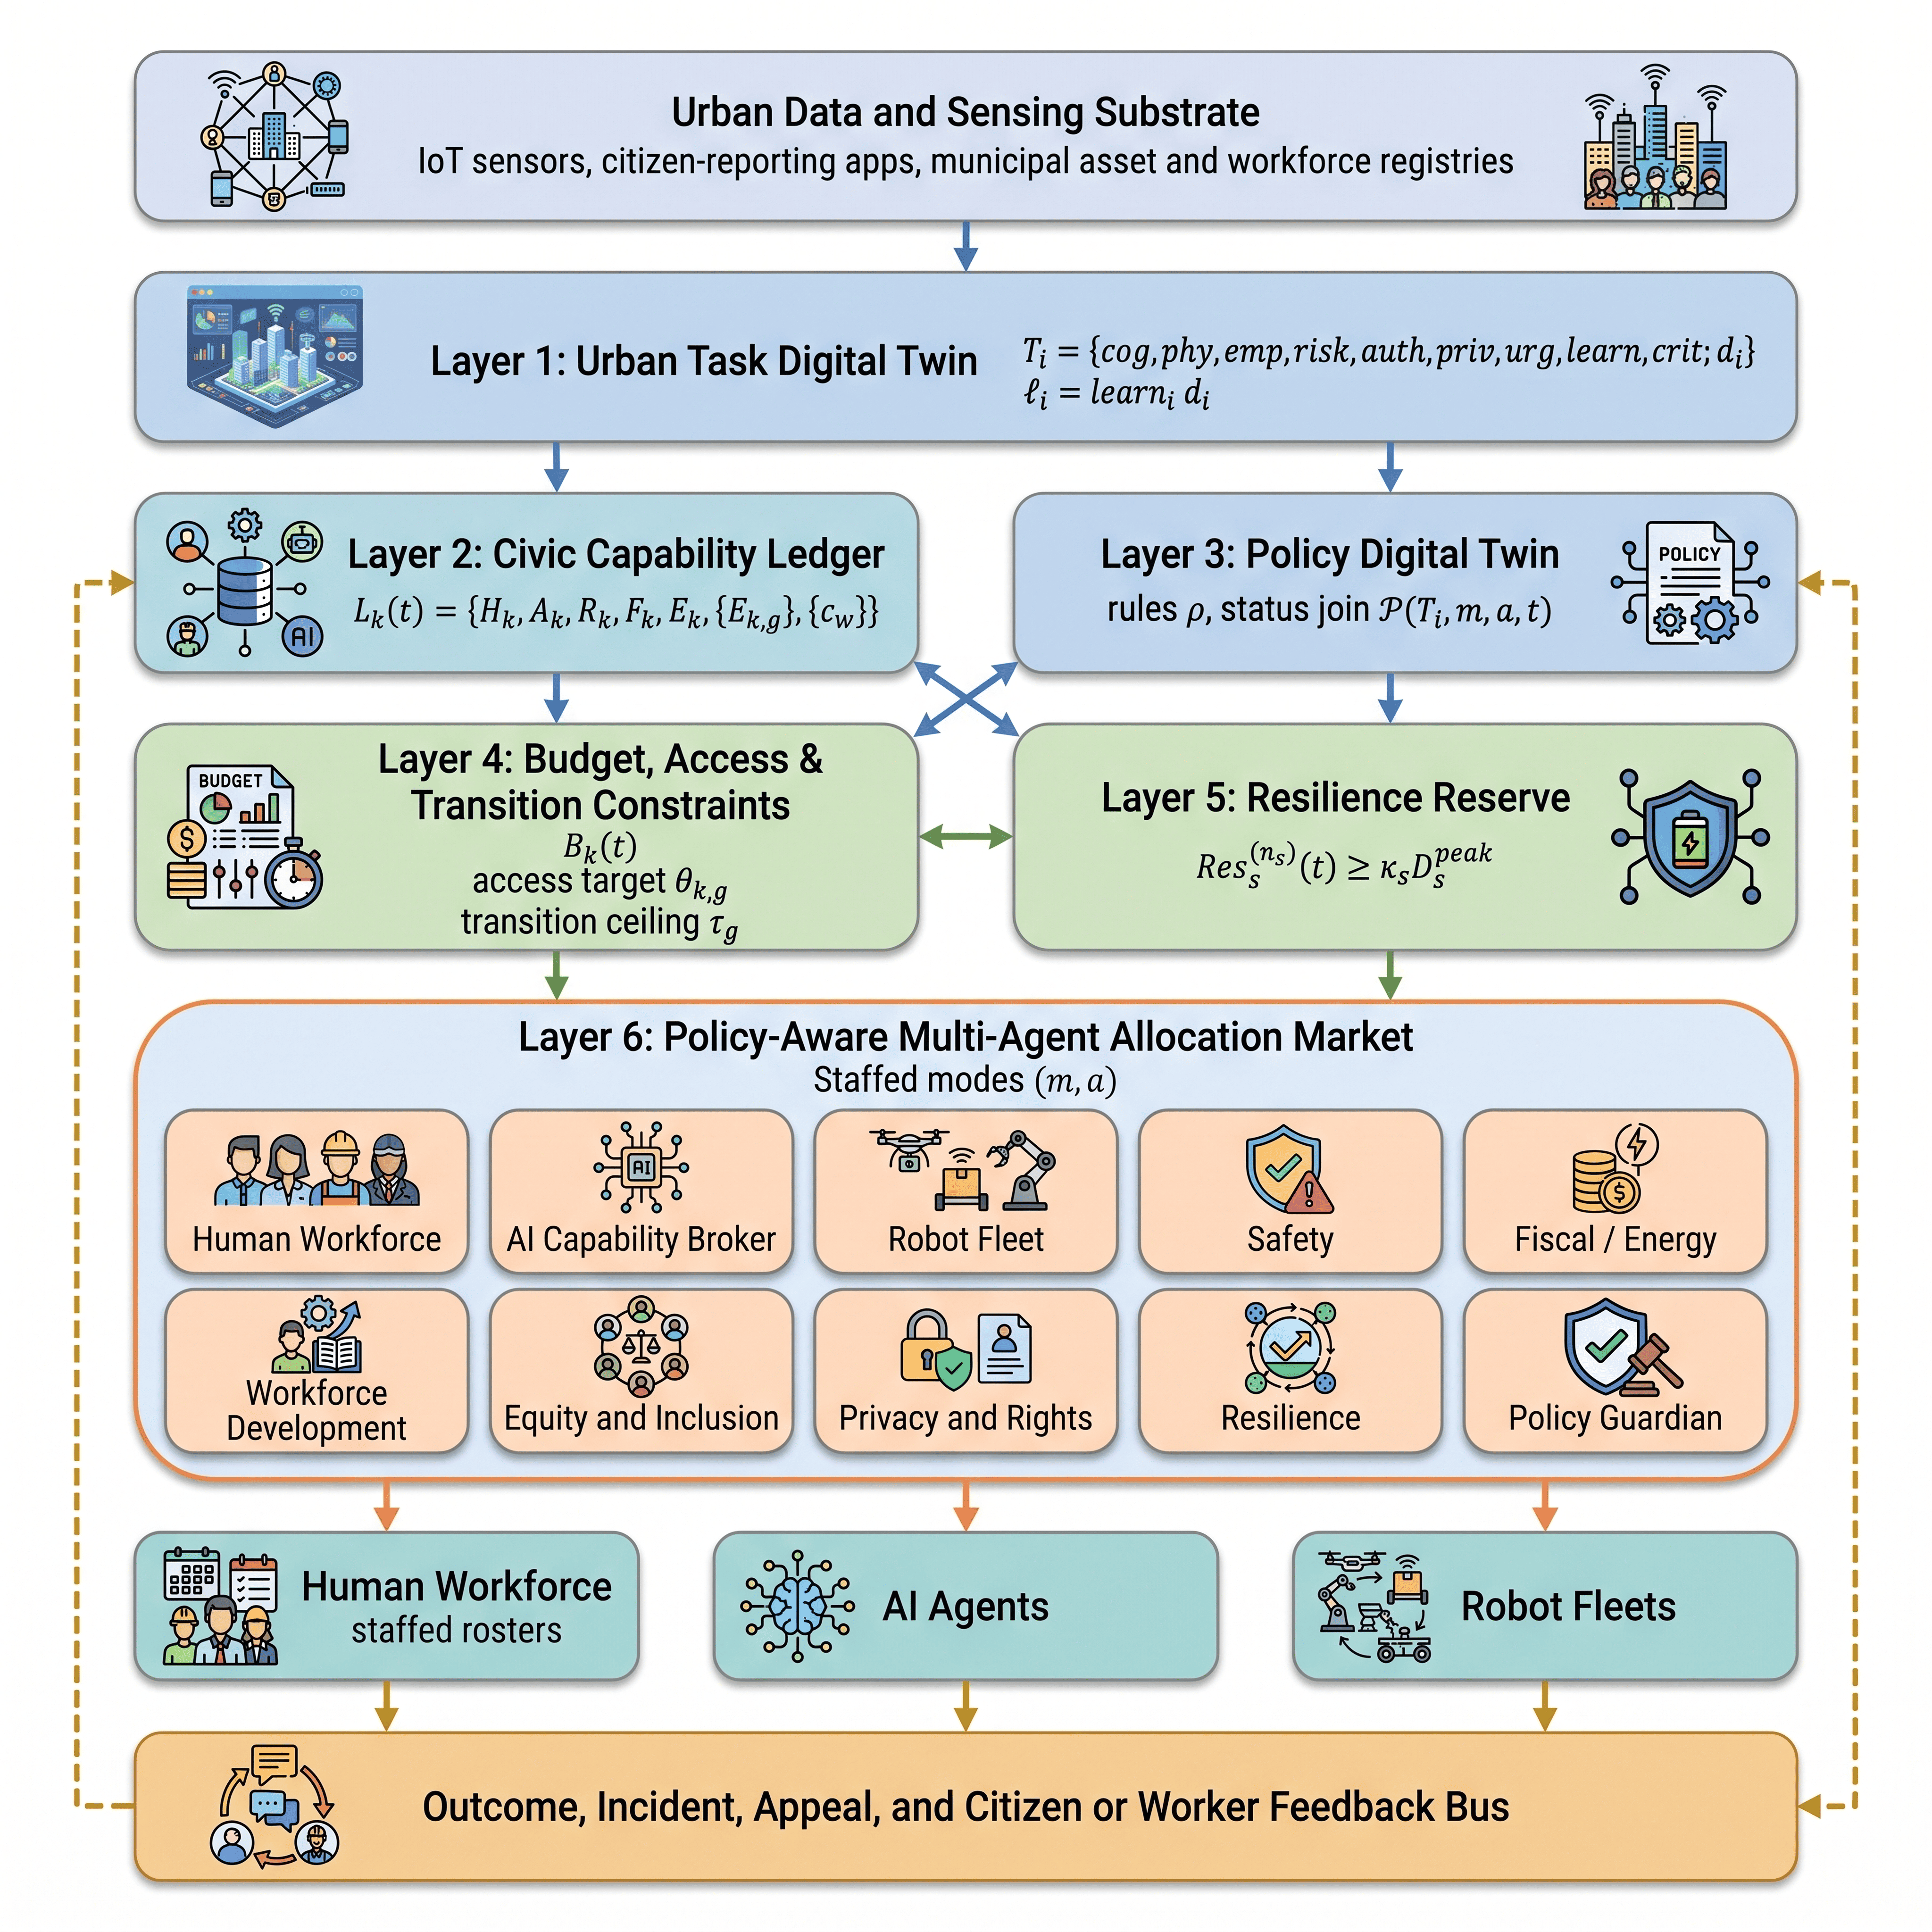
\includegraphics[width=\linewidth]{images/arch}
		\caption{\DIFaddFL{Reference architecture of CivicWorkOS, read top to bottom. Solid arrows are the forward allocation path from sensed urban data through the governance layers to execution; the ten agents are drawn inside the market because they constitute it. The Ledger supplies fallback capacity $F_k$ of Equation~\eqref{eq:fallback} to the reserve through Equation~\eqref{eq:cs}, and per-practitioner practice totals $c_w$ to the career-stage test of Equation~\eqref{eq:stage}. The Policy Twin supplies the replacement factor $\eta_k$, the access target $\theta_{k,g}$, and the roster guards that restrict $\mathcal{A}_{i,m}$. Dashed arrows are the outcome-feedback path, which updates both governance services.}}
		\label{fig:architecture}
	\end{figure}

	\DIFaddend \subsection{Layer 6: Policy-Aware Multi-Agent Allocation Market}
	\label{sec:layer6}

	Ten specialized agents \DIFdelbegin \DIFdel{propose and }\DIFdelend price candidate staffed modes\DIFdelbegin \DIFdel{. Five are }\DIFdelend \DIFaddbegin \DIFadd{: five }\DIFaddend \textit{capability agents} \DIFdelbegin \DIFdel{estimating what a staffed mode can do (the Human Workforce Agent, AI Capability Broker, Robot Fleet Agent, Safety Agent, and Fiscal and Energy Agent), and five are }\DIFdelend \DIFaddbegin \DIFadd{estimate the flow terms and five }\DIFaddend \textit{civic agents} \DIFdelbegin \DIFdel{estimating what it costs the city in stocks it must later replenish: the Workforce Development Agent ($\phi_m$, $\psi_a$, $D^{skill}$), the Equity and Inclusion Agent ($Eq^{srv}$, $D^{trans}$, and the group shares in~\eqref{eq:accessshare}), the Privacy and Rights Agent ($Pr$), the Resilience Agent ($D^{fall}$, $Res^{(n_s)}_s$), and the }\DIFdelend \DIFaddbegin \DIFadd{the stock changes, among them the }\DIFaddend Policy Guardian Agent, which executes~\eqref{eq:policy} and holds \DIFdelbegin \DIFdel{veto authority. All ten appear in }\DIFdelend \DIFaddbegin \DIFadd{a veto (}\DIFaddend Figure~\ref{fig:architecture}\DIFdelbegin \DIFdel{, and the two-family split is the architectural expression of the flow and stock separation of Section~\ref{sec:problem}. }%DIFDELCMD < 

%DIFDELCMD < 	%%%
\DIFdel{The market protocol }\DIFdelend \DIFaddbegin \DIFadd{). The market }\DIFaddend is a single-round sealed-bid call, \DIFdelbegin \DIFdel{not an iterated negotiation, and this is deliberate. The Policy Guardian Agent publishes the task and the surviving roster set. Each agent returns its terms for every surviving staffed mode within a fixed deadline, with a declared default used where an agent does not answer in time. The auctioneer computes~\eqref{eq:scv} and~\eqref{eq:aug}, applies the admissibility test~\eqref{eq:admis}, and awards. No agent sees another's bid before submitting, so there is no bidding dynamic to converge, and the per-task decision terminates in one round with a bounded number of queries. The market is therefore a structured elicitation and pricing }\DIFdelend \DIFaddbegin \DIFadd{a structured elicitation }\DIFaddend mechanism rather than a strategic game, and we make no equilibrium claim for it. \DIFdelbegin \DIFdel{Section~\ref{sec:limitations} }\DIFdelend \DIFaddbegin \DIFadd{Appendix~\ref{app:framework-market} lists the agents and the protocol, and Section~\ref{sec:threats} }\DIFaddend records the principal--agent exposure \DIFdelbegin \DIFdel{this }\DIFdelend \DIFaddbegin \DIFadd{the }\DIFaddend design leaves open\DIFdelbegin \DIFdel{, which is the reason the terms most vulnerable to strategic reporting are cross-validated against independently observed outcomes.
	}%DIFDELCMD < 

%DIFDELCMD < 	%%%
\DIFdelend \DIFaddbegin \DIFadd{.
	}\DIFaddend \section{Architecture, Optimization Program, and Algorithm}
	\label{sec:architecture}

	\subsection{Reference Architecture}
	\label{sec:refarch}

	Figure~\ref{fig:architecture} realizes the layers of Section~\ref{sec:framework} as \DIFdelbegin \DIFdel{a deployable system . Sensed data, citizen reports, and municipal registries feed the Urban Task Digital Twin, which encodes each unit of work as~\eqref{eq:task} and publishes it to two parallel governance services, the Civic Capability Ledger and the Policy Digital Twin. Both condition both constraint modules. The ledger supplies the pipeline and composition state sizing $B_k(t)$, the per-practitioner totals $c_w(t)$ that determine career stage through~\eqref{eq:stage}, and the fallback capacity $F_k(t)$ that enters $C_s(t)$ through~\eqref{eq:cs}. The policy twin supplies the parameters $\eta_k$, $B_k^{min}$, $\theta_{k,g}$, $\kappa_s$, and $n_s$ those constraints are evaluated against, and the roster guards that restrict $\mathcal{A}_{i,m}$. The Allocation Market consumes all four outputs, prices candidate staffed modes through its ten agents, and dispatches work. A }\DIFdelend \DIFaddbegin \DIFadd{an event-driven system in which a }\DIFaddend single feedback bus returns outcomes, incidents, \DIFdelbegin \DIFdel{appeals, and citizen or worker feedback }\DIFdelend \DIFaddbegin \DIFadd{and appeals }\DIFaddend from all three execution channels to both governance services\DIFdelbegin \DIFdel{, as~\eqref{eq:ledger} requires: the ledger holds robot and AI capability terms that cannot be maintained if machine outcomes bypass it, and compliance monitoring depends on human outcomes as much as machine ones. }%DIFDELCMD < 

%DIFDELCMD < 	%%%
\DIFdel{The architecture is event-driven. Governance services run persistently behind a publish and subscribe bus, the market instantiates a short-lived per-task call, and the rebalancing solver runs as a scheduled batch job. Robot execution interfaces with }\DIFdelend \DIFaddbegin \DIFadd{. Robot execution sits behind }\DIFaddend fleet middleware enforcing ISO~10218-2\DIFdelbegin \DIFdel{:2025~\mbox{%DIFAUXCMD
\cite{ISO2025b} }\hskip0pt%DIFAUXCMD
at the cell and application level, and the robots themselves conform }\DIFdelend \DIFaddbegin \DIFadd{~}\citep{ISO2025b}\DIFadd{, with the robots conforming }\DIFaddend to ISO~10218-1\DIFdelbegin \DIFdel{:2025~\mbox{%DIFAUXCMD
\cite{ISO2025}}\hskip0pt%DIFAUXCMD
, independently of the allocation decision, }\DIFdelend \DIFaddbegin \DIFadd{~}\citep{ISO2025}\DIFadd{, }\DIFaddend so a policy-level error cannot defeat a hardware-level safety interlock.

	\DIFdelbegin %DIFDELCMD < \begin{figure}[!htbp]
%DIFDELCMD < 		\centering
%DIFDELCMD < 		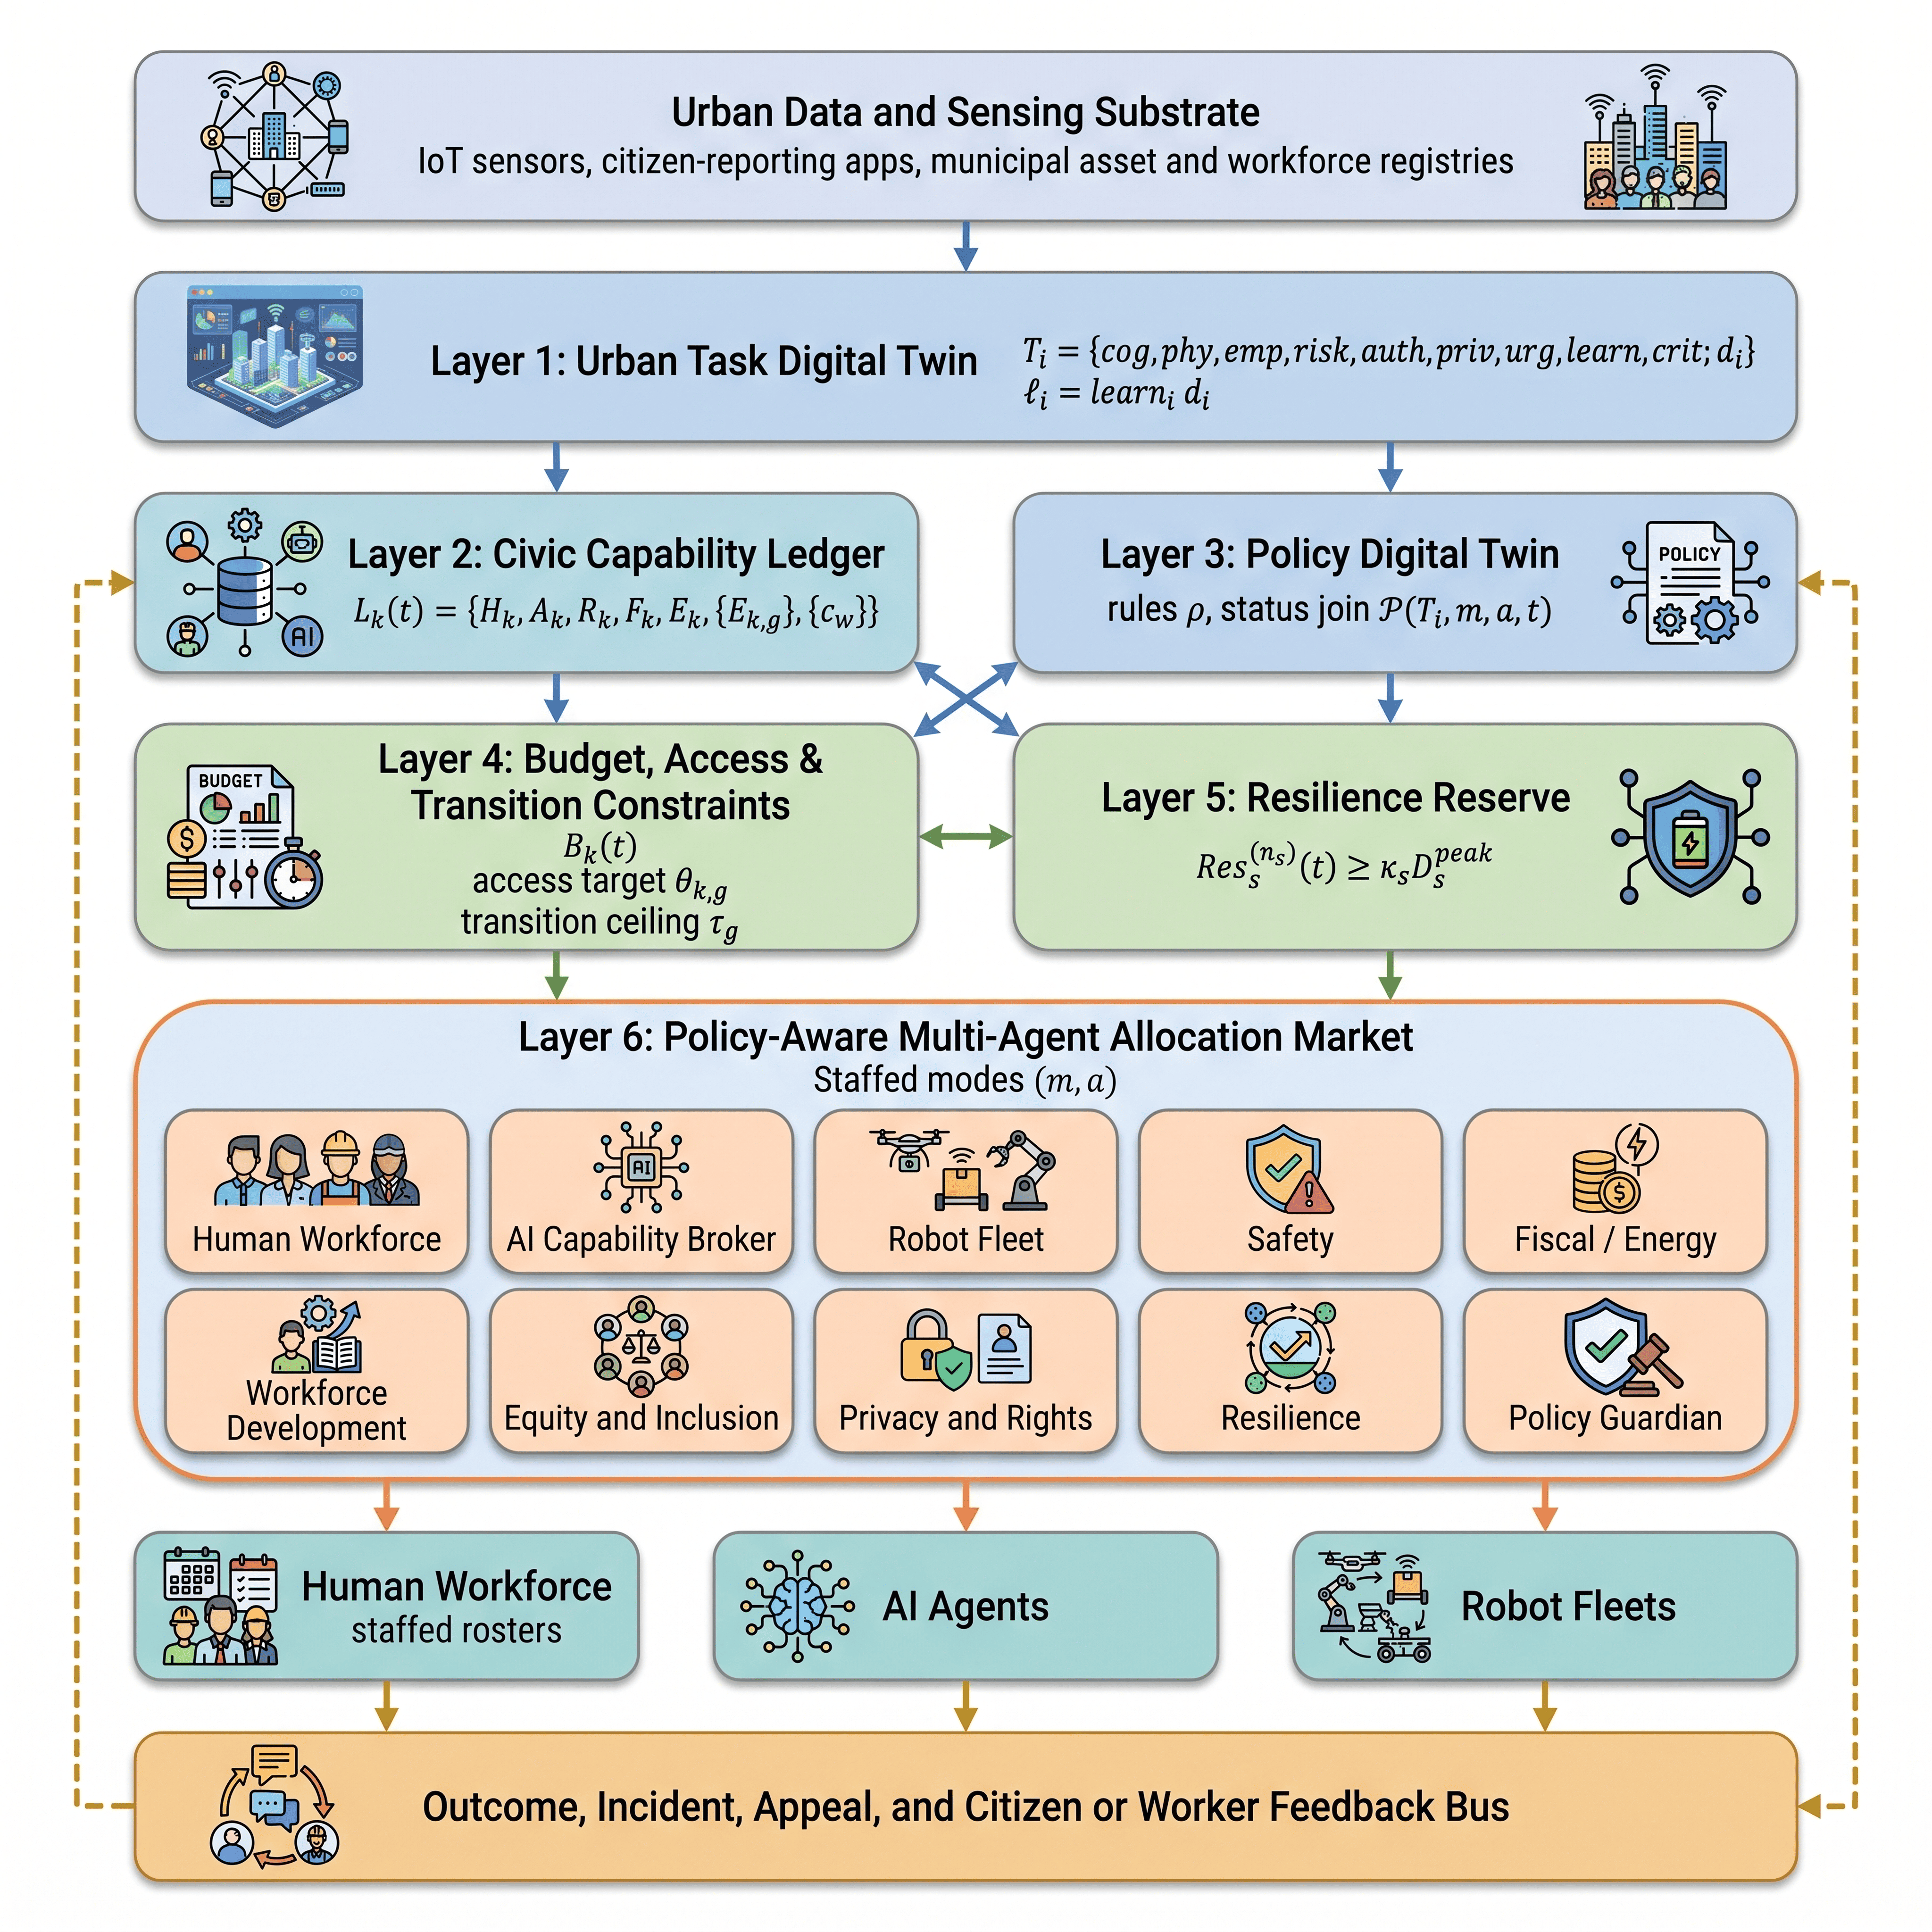
\includegraphics[width=\linewidth]{images/arch}
%DIFDELCMD < 		%%%
%DIFDELCMD < \caption{%
{%DIFAUXCMD
\DIFdelFL{Reference architecture of CivicWorkOS, read top to bottom. Solid arrows are the forward allocation path from sensed urban data through the governance layers to execution; the ten agents are drawn inside the market because they constitute it. The Ledger supplies fallback capacity $F_k$ of Equation~\eqref{eq:fallback} to the reserve through Equation~\eqref{eq:cs}, and per-practitioner practice totals $c_w$ to the career-stage test of Equation~\eqref{eq:stage}. The Policy Twin supplies the replacement factor $\eta_k$, the access target $\theta_{k,g}$, and the roster guards that restrict $\mathcal{A}_{i,m}$. Dashed arrows are the outcome-feedback path, which updates both governance services.}}
		%DIFAUXCMD
%DIFDELCMD < \label{fig:architecture}
%DIFDELCMD < 	\end{figure}
%DIFDELCMD < 	

%DIFDELCMD < 	%%%
\DIFdelend \subsection{Runtime Allocation Workflow}
	\label{sec:workflow}

	Figure~\ref{fig:workflow} shows the per-task control flow that Algorithm~\ref{alg:scv} formalizes\DIFdelbegin \DIFdel{: encode the task, query the policy twin per mode, build and prune the roster set according to the returned status, price each surviving staffed mode by~\eqref{eq:cad} and~\eqref{eq:scv}, apply the admissibility test of Section~\ref{sec:online}, and execute the arg max on the Lagrangian-augmented score. Three properties matter. Policy filtering is per mode and roster pruning is per roster, as~\eqref{eq:policy} and the }\textit{\DIFdel{restrict}} %DIFAUXCMD
\DIFdel{status require. Either stage may empty the }\DIFdelend \DIFaddbegin \DIFadd{. If policy filtering or roster pruning empties the }\DIFaddend candidate set, \DIFdelbegin \DIFdel{in which case }\DIFdelend the task routes to Zone\DIFaddbegin \DIFadd{~}\DIFaddend Z4 human-reserved execution \DIFdelbegin \DIFdel{rather than leaving the arg max undefined, and that }\DIFdelend \DIFaddbegin \DIFadd{and the }\DIFaddend event is counted, because its rate is the operational price of the constraint system\DIFdelbegin \DIFdel{and is reported as a metric in Section~\ref{sec:metrics}.
	And the ledger update writes both the domain accrual $\Lambda_k$ and the per-practitioner totals $c_w$, since only the second can move a practitioner across the career-stage boundary of~\eqref{eq:stage}.
	}\DIFdelend \DIFaddbegin \DIFadd{.
	}\DIFaddend 

	\begin{figure}[!htbp]
		\centering
		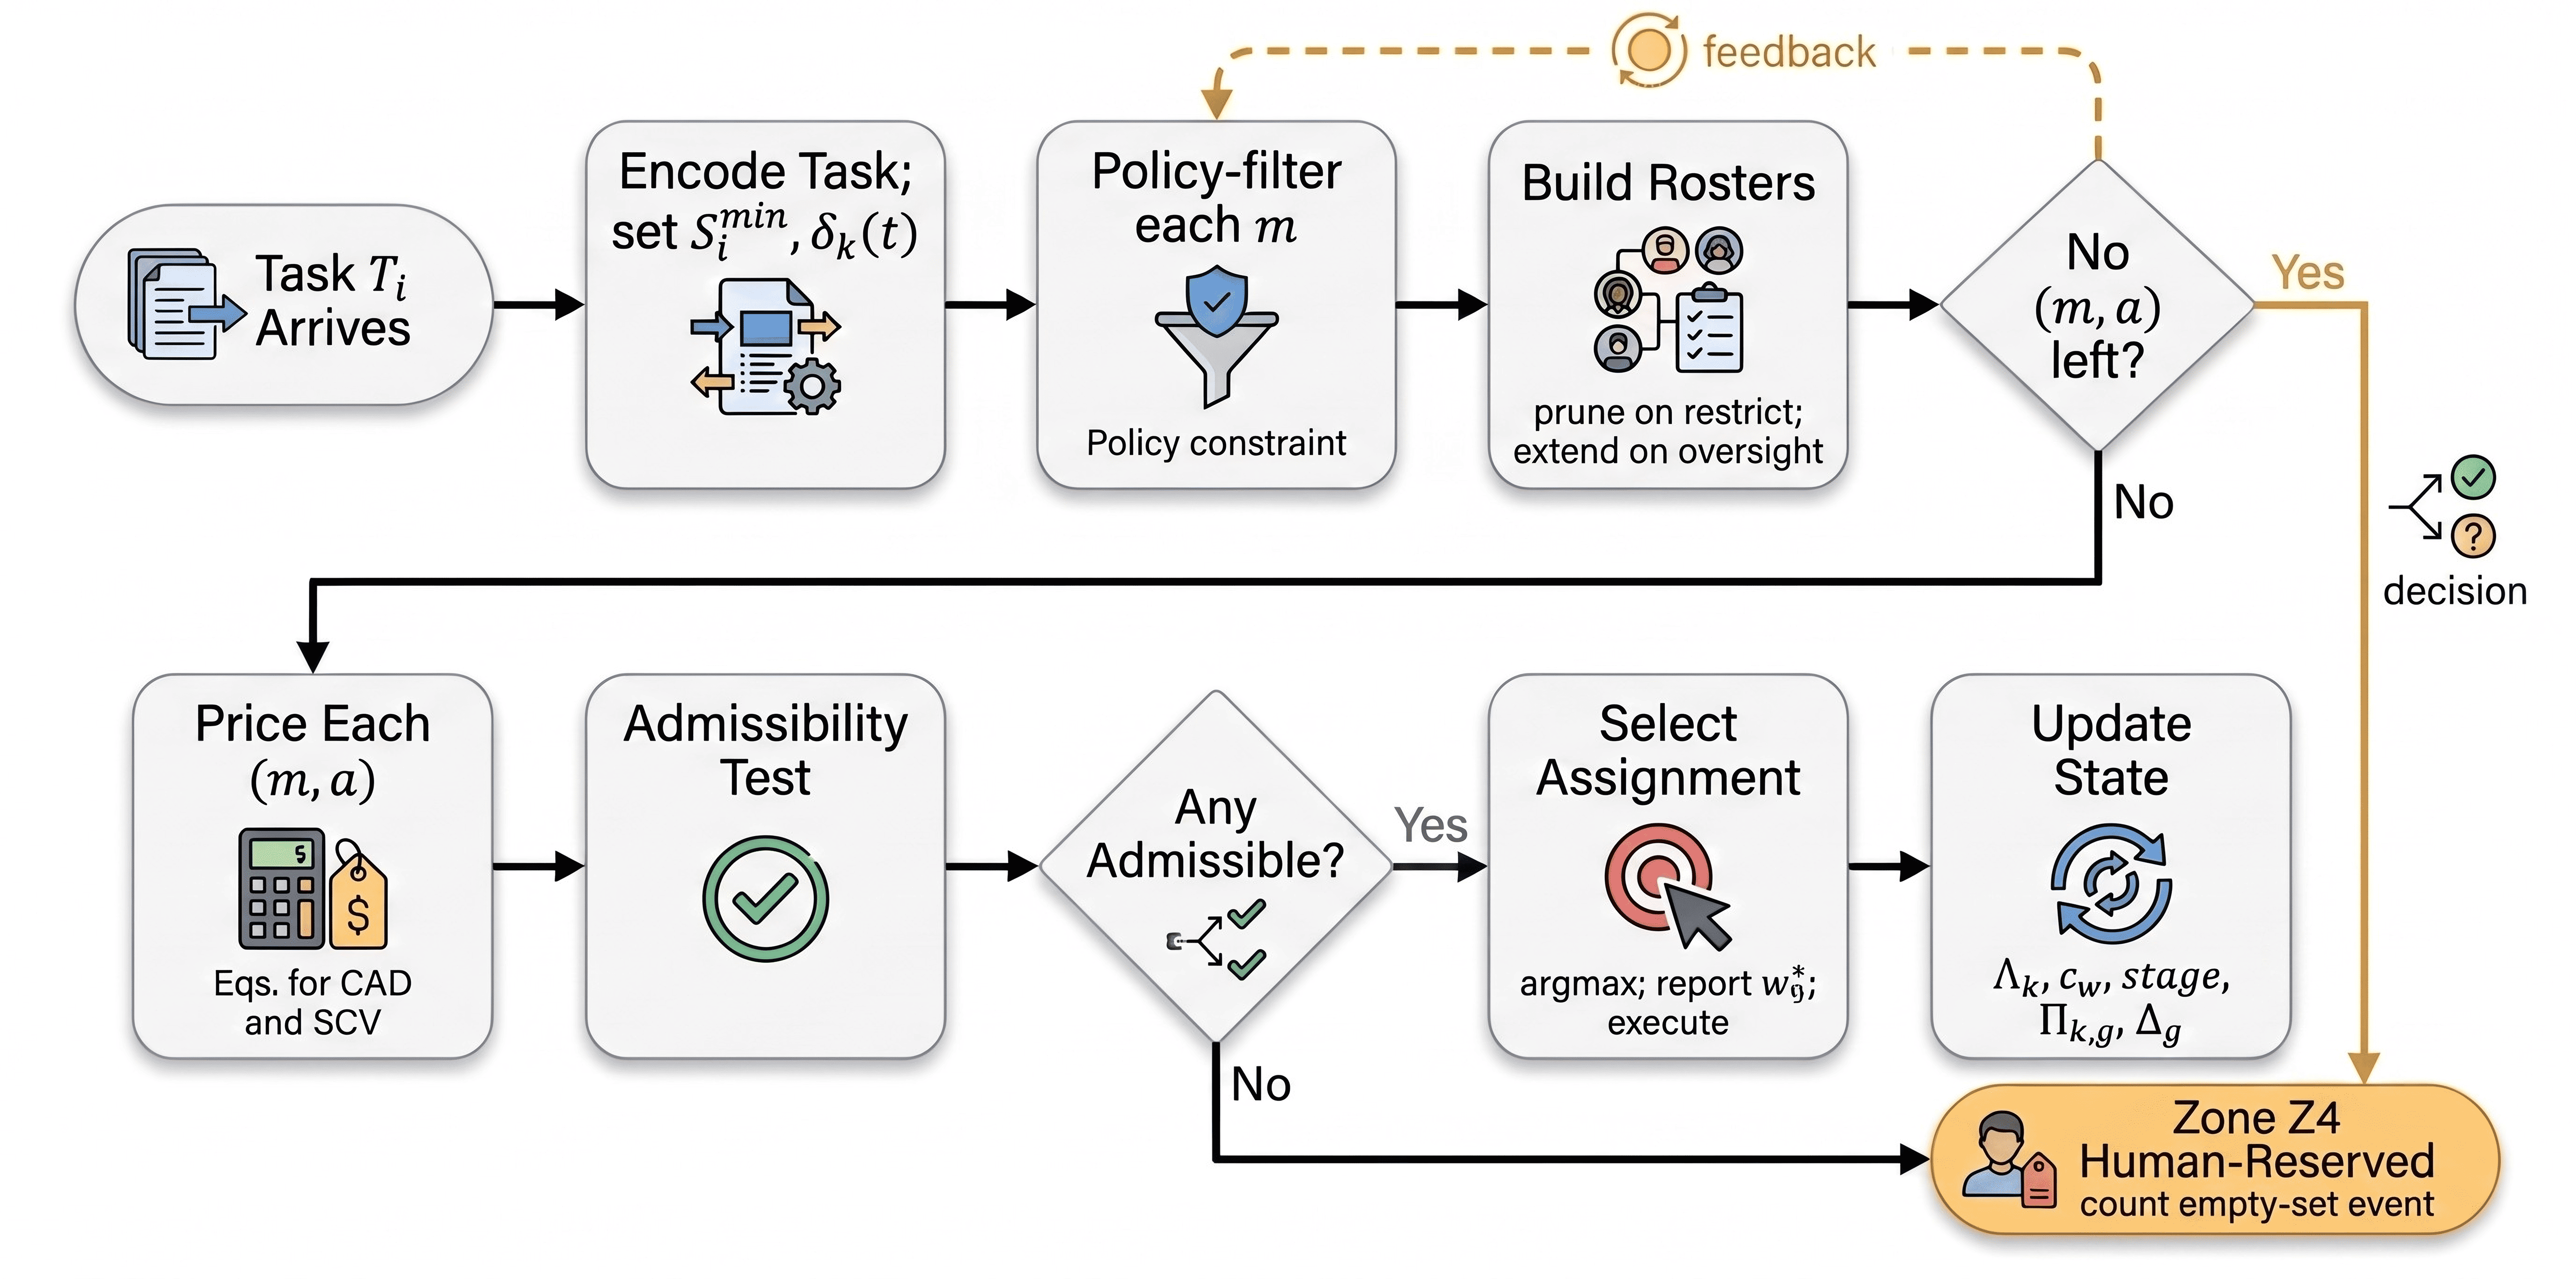
\includegraphics[width=\linewidth]{images/runtime}
		\caption{Runtime allocation workflow, matching Algorithm~\ref{alg:scv}. The upper row encodes the task, sets the safety floor and the catch-up increment, policy-filters modes, and builds the roster set, pruning it where the twin returns \textit{restrict} and extending it with a named reviewer where it returns \textit{allow-with-oversight}. The lower row prices the surviving staffed modes, applies the admissibility test~\eqref{eq:admis}, and either falls back to Zone Z4 or selects and executes. The dashed edge returns outcomes to the Policy Digital Twin, which is what makes the zone-transition predicates (Section~\ref{sec:zones}) evaluable.}
		\label{fig:workflow}
	\end{figure}

	\subsection{Sustainable Civic Value (SCV)}
	\label{sec:math}

	For each task $T_i$ and staffed mode $(m,a)$, the \textit{Sustainable Civic Value} is given by equation~\eqref{eq:scv}:
	\begin{equation}
		\begin{split}
			SCV_{i,m,a} =\;&
			w_1 Q_{i,m,a}
			+w_2 S_{i,m,a}
			+w_3 P_{i,m,a}
			+w_4 Eq^{srv}_{i,m,a}
			+w_5 Tr_{i,m,a}\\
			&-w_6 Cost_{i,m,a}
			-w_7 En_{i,m}
			-w_8 Pr_{i,m}
			-w_9 CAD_{i,m,a},
		\end{split}
		\label{eq:scv}
	\end{equation}
	where $Q$ is service quality, $S$ safety, $P$ productivity, $Eq^{srv}$ the equity of service delivery across resident groups\DIFdelbegin \DIFdel{and districts}\DIFdelend , $Tr$ agent trust, $Cost$ operating cost, $En$ energy use, $Pr$ privacy risk, and $CAD$ the debt of~\eqref{eq:cad}. The first eight terms are flows \DIFdelbegin \DIFdel{measured }\DIFdelend on the task's execution window \DIFdelbegin \DIFdel{, }\DIFdelend and the ninth \DIFdelbegin \DIFdel{is }\DIFdelend a change in municipal stocks\DIFdelbegin \DIFdel{. Six terms }\DIFdelend \DIFaddbegin \DIFadd{; six }\DIFaddend depend on the roster as well as the mode\DIFdelbegin \DIFdel{, because staffing a developing practitioner alongside a competent lead changes the quality, safety, productivity, trust, and cost of the execution as well as its developmental content.
	Section~\ref{sec:problem} argued why no capability-formation, resilience-contribution, or accountability term appears separately, and Section~\ref{sec:config} reports the effective weight each civic construct receives once $w_9$ and the debt weights are composed.
	}\DIFdelend \DIFaddbegin \DIFadd{.
	}\DIFaddend 

	\DIFdelbegin \DIFdel{Weighting a multi-criteria score linearly }\DIFdelend \DIFaddbegin \DIFadd{A linear weighting }\DIFaddend trades flexibility for interpretability \DIFdelbegin \DIFdel{and tractability relative to explicit }\DIFdelend \DIFaddbegin \DIFadd{relative to }\DIFaddend Pareto-front methods~\DIFdelbegin \DIFdel{\mbox{%DIFAUXCMD
\cite{Osika2023,ZhengRasheed2026}}\hskip0pt%DIFAUXCMD
. One consequence must be stated here rather than deferred, because it bears on the democratic claims of Section~\ref{sec:feedback}. A linear scalarization }\DIFdelend \DIFaddbegin \citep{Osika2023,ZhengRasheed2026}\DIFadd{, and }\DIFaddend recovers only solutions on the convex hull of the attainable set, \DIFdelbegin \DIFdel{so allocations in non-convex regions of the Pareto frontier are unreachable for }\textit{\DIFdel{every}} %DIFAUXCMD
\DIFdel{weight vector~\mbox{%DIFAUXCMD
\cite{Osika2023}}\hskip0pt%DIFAUXCMD
. If a socially preferred compromise lies in such a region, no deliberation over $w_1,\ldots,w_9$ can select it, and the panelwould be exercising authority over a strictly smaller set of outcomes than it appears to. Section~\ref{sec:limitations} records this restriction with the alternatives that would remove it. }%DIFDELCMD < 

%DIFDELCMD < 	%%%
\subsubsection*{\DIFdel{Normalization}}
	%DIFAUXCMD
%DIFDELCMD < 

%DIFDELCMD < 	%%%
\DIFdel{The nine terms have incompatible native units, so each is }\DIFdelend \DIFaddbegin \DIFadd{which bounds the panel's authority (Section~\ref{sec:feedback}). All nine terms are }\DIFaddend rescaled to $[0,1]$\DIFdelbegin \DIFdel{before weighting, and the two families are rescaled differently. For the eight }\textit{\DIFdel{flow}} %DIFAUXCMD
\DIFdel{terms we use min--max normalization }\DIFdelend \DIFaddbegin \DIFadd{: the flow terms }\DIFaddend against a trailing twelve-month \DIFaddbegin \DIFadd{window}\DIFaddend , \DIFdelbegin \DIFdel{sector-specific window, refreshed so the scale adapts as practice improves. That would be wrong for the debt components : if $D^{skill}$ and $D^{fall}$ were normalized against }\DIFdelend \DIFaddbegin \DIFadd{and the debt components against externally fixed denominators, since against }\DIFaddend a rolling window \DIFdelbegin \DIFdel{, then as the pipeline decayed the reference range would decay with it, normalized scores would stay comfortably }\DIFdelend \DIFaddbegin \DIFadd{a decaying pipeline would keep scoring }\DIFaddend mid-range \DIFdelbegin \DIFdel{, and a framework premised on a city looking efficient while its capability empties out would have built an instrument that cannot see the emptying}\DIFdelend \DIFaddbegin \DIFadd{(Appendix~\ref{app:proofs-anchors})}\DIFaddend .

	\DIFdelbegin \DIFdel{The five debt components therefore carry no windowed normalization at all. Each is constructed as a ratio whose denominator is fixed externally, which places each debt term in $[0,1]$ as defined in equation~\eqref{eq:anchors}:
	}\begin{displaymath}
		\DIFdel{\begin{aligned}
			D^{skill}_{i,m,a} &= 1-\phi_m\psi_a &&\text{against the task's own full developmental content } \ell_i,\\
			D^{fall}_{i,m} &= \min\!\Big(1,\ \Delta F_{\kappa(i)}(m)\,/\,\rho_{\sigma(i)}\Big) &&\text{against the statutory reserve } \rho_s=\kappa_s D^{peak}_s,\\
			D^{acct}_{i,m} &= crit_i \cdot n^{unacct}_{i,m}/n^{steps}_{i,m} &&\text{against the decision-step count of the task},\\
			D^{dep}_{i,m} &= n^{single}_{i,m}/n^{auto}_{i,m} &&\text{against the automated-input count of the mode},\\
			D^{trans}_{i,m} &= \textstyle\sum_{g}\varpi_{g}(i,m)\,\bigl(1-\chi_g\bigr) &&\text{against funded transition coverage } \chi_g,
		\end{aligned}
		%DIFDELCMD < \label{eq:anchors}%%%
	}\end{displaymath}%DIFAUXCMD
%DIFDELCMD < 	%%%
\DIFdel{where $\Delta F_k(m)$ is the fallback reduction mode $m$ would cause if generalized across the domain and $\varpi_g(i,m)$ is group $g$'s share of the workers whose allocated hours the mode reduces. All five denominators are external to observed performance, so a decade of decline registers as a decade of decline. Note that $D^{trans}$ is anchored to the reskilling coverage $\chi_g$ and not to the displacement ceiling $\tau_g$: the ceiling is a hard constrainton $\Delta_g$, and the priced quantity is the unfunded share of the burden}\DIFdelend \DIFaddbegin \subsubsection*{\DIFadd{Default Weights and What They Actually Carry}}
	\label{sec:weights}

	\DIFadd{The illustrative weights are $w_1{=}0.15$ (quality), $w_2{=}0.18$ (safety), $w_3{=}0.14$ (productivity), $w_4{=}0.10$ (service equity), $w_5{=}0.05$ (trust), $w_6{=}0.08$ (cost), $w_7{=}0.03$ (energy), $w_8{=}0.05$ (privacy risk), and $w_9{=}0.22$ (CAD), with debt weights $\alpha{=}0.28$, $\beta{=}0.22$, $\gamma{=}0.18$, $\delta{=}0.12$, and $\epsilon{=}0.20$. They are design defaults for the panel to revise, not fitted estimates; Table~\ref{tab:app-params} assigns a default to every remaining parameter.
}

	\DIFadd{Table~\ref{tab:weights} reports the }\textit{\DIFadd{effective}} \DIFadd{weight each construct carries once the weights are composed, because a weight vector can assert a priority the arithmetic withholds. The deferred block carries 0.22, more than productivity at 0.14, but the largest single construct is safety at 0.180: CAD carries the largest weight as a block and as no component. Labor-transition burden carries only 0.044, deliberately: an objective weight can be outvoted, so transition is also carried by the hard constraint~\eqref{eq:justtransition}, and a city that judges displacement unacceptable lowers $\tau_g$ rather than raising $w_9\epsilon$. Proposition~\ref{prop:price} shows which lever is deciding}\DIFaddend .

	\DIFaddbegin \begin{table}[!htbp]
		\caption{\DIFaddFL{Effective weight of each construct in the CivicWorkOS default configuration, obtained by composing $w_9=0.22$ with the debt weights. The deferred block is the largest single block of the objective; safety is the largest single construct. Column sums to 1.000.}}
		\label{tab:weights}
		\begin{tabular}{@{}llc@{}}
			\toprule
			\textbf{\DIFaddFL{Construct}} & \textbf{\DIFaddFL{Enters via}} & \textbf{\DIFaddFL{Effective weight}}\\
			\midrule
			\DIFaddFL{Safety }& \DIFaddFL{$w_2$ }& \DIFaddFL{0.180}\\
			\DIFaddFL{Service quality }& \DIFaddFL{$w_1$ }& \DIFaddFL{0.150}\\
			\DIFaddFL{Productivity }& \DIFaddFL{$w_3$ }& \DIFaddFL{0.140}\\
			\DIFaddFL{Service equity (residents) }& \DIFaddFL{$w_4$ }& \DIFaddFL{0.100}\\
			\DIFaddFL{Operating cost }& \DIFaddFL{$w_6$ }& \DIFaddFL{0.080}\\
			\DIFaddFL{Skill formation }& \DIFaddFL{$w_9\alpha$ }& \DIFaddFL{0.062}\\
			\DIFaddFL{Trust }& \DIFaddFL{$w_5$ }& \DIFaddFL{0.050}\\
			\DIFaddFL{Privacy risk }& \DIFaddFL{$w_8$ }& \DIFaddFL{0.050}\\
			\DIFaddFL{Fallback capacity }& \DIFaddFL{$w_9\beta$ }& \DIFaddFL{0.048}\\
			\DIFaddFL{Labor-transition burden (workers) }& \DIFaddFL{$w_9\epsilon$ }& \DIFaddFL{0.044}\\
			\DIFaddFL{Accountability }& \DIFaddFL{$w_9\gamma$ }& \DIFaddFL{0.040}\\
			\DIFaddFL{Energy }& \DIFaddFL{$w_7$ }& \DIFaddFL{0.030}\\
			\DIFaddFL{Vendor dependency }& \DIFaddFL{$w_9\delta$ }& \DIFaddFL{0.026}\\
			\midrule
			\textit{\DIFaddFL{Deferred block total}} & \DIFaddFL{$w_9$ }& \textit{\DIFaddFL{0.220}}\\
			\bottomrule
		\end{tabular}
	\end{table}

	\DIFaddend \subsection{The City-Wide Allocation Program}
	\label{sec:program}

	The constraints of Sections~\ref{sec:hcpb} through~\ref{sec:layer5} couple decisions across tasks\DIFdelbegin \DIFdel{: whether one inspection may go to an unstaffed autonomous team depends on how much practice the domain's other inspections have already delivered, and to whom. A per-task rule cannot by itself guarantee feasibility, so the program it approximates must be written down. Over }\DIFdelend \DIFaddbegin \DIFadd{, so over }\DIFaddend a rebalancing window \DIFdelbegin \DIFdel{containing task set $\mathcal{T}(\Delta T)$, CivicWorkOS solves the programformulated in equation~\eqref{eq:program}(with objective~\eqref{eq:prog-obj} and constraints~\eqref{eq:prog-assign}--\eqref{eq:prog-cap})}\DIFdelend \DIFaddbegin \DIFadd{CivicWorkOS solves program~\eqref{eq:program}}\DIFaddend :
	\begin{subequations}
		\label{eq:program}
		\begin{align}
			\max_{\mathbf{x},\boldsymbol{\varsigma}} \quad & \sum_{i \in \mathcal{T}(\Delta T)} \sum_{m \in \mathcal{M}} \sum_{a\in\mathcal{A}_{i,m}} x_{i,m,a}\, SCV_{i,m,a} \;-\; M \sum_{k,g}\varsigma_{k,g}
			\label{eq:prog-obj}\\
			\text{s.t.}\quad
			& \textstyle\sum_{m} \sum_{a} x_{i,m,a} = 1, && \forall i,
			\label{eq:prog-assign}\\
			& x_{i,m,a} = 0 \ \text{ if } \mathcal{P}(T_i,m,a,t)=\textit{prohibit},
			\label{eq:prog-policy}\\
			& x_{i,m,a} = 0 \ \text{ if } S_{i,m,a} < S^{min}_i,
			\label{eq:prog-safety}\\
			& \textstyle\sum_{i \in \mathcal{T}_k} \sum_{m}\sum_{a} x_{i,m,a}\,\ell_i\,\phi_m\,\psi_a \geq B_k(t), && \forall k,
			\label{eq:prog-hcpb}\\
			& \Pi_{k,g}(\mathbf{x}) + \varsigma_{k,g} \geq \theta_{k,g} - \varepsilon_k, \quad \varsigma_{k,g}\geq 0, && \forall k,g,
			\label{eq:prog-access}\\
			& \Delta_g(\mathbf{x}) \leq \tau_g, && \forall g,
			\label{eq:prog-just}\\
			& Res^{(n_s)}_s(\mathbf{x}) \geq \kappa_s D^{peak}_s, && \forall s,
			\label{eq:prog-res}\\
			& \textstyle\sum_{i}\sum_{m}\sum_{a} x_{i,m,a}\, u_{i,m,a,r} \leq U_r, && \forall r,
			\label{eq:prog-cap}\\
			& x_{i,m,a} \in \{0,1\}.
			\label{eq:prog-int}
		\end{align}
	\end{subequations}
	Here $u_{i,m,a,r}$ is the consumption of resource $r$ (human hours by grade and stage, \DIFdelbegin \DIFdel{robot-fleet hoursby class, AI }\DIFdelend \DIFaddbegin \DIFadd{fleet hours, }\DIFaddend inference budget) \DIFdelbegin \DIFdel{that staffed mode $(m,a)$ implies for task $i$, }\DIFdelend and $U_r$ its availability. The access constraint \DIFdelbegin \DIFdel{~\eqref{eq:prog-access} }\DIFdelend carries an elastic slack \DIFdelbegin \DIFdel{$\varsigma_{k,g}$ }\DIFdelend penalized at a large $M$\DIFdelbegin \DIFdel{in the objective}\DIFdelend , so an unattainable \DIFdelbegin \DIFdel{composition target degrades into }\DIFdelend \DIFaddbegin \DIFadd{target yields }\DIFaddend a published shortfall rather than \DIFdelbegin \DIFdel{into infeasibility , and no individual assignmentis ever compelled by the target alone. }\DIFdelend \DIFaddbegin \DIFadd{infeasibility and never compels an individual assignment, which }\DIFaddend Section~\ref{sec:legality} \DIFdelbegin \DIFdel{explains why that elasticity is }\DIFdelend \DIFaddbegin \DIFadd{shows to be }\DIFaddend a legal requirement\DIFdelbegin \DIFdel{and not only a numerical convenience. The roster dimension is what makes~\eqref{eq:prog-cap} bind on individual practitioners rather than on an anonymous pool, and it is what makes~\eqref{eq:prog-access} evaluable at all. Program~\eqref{eq:program} is }\DIFdelend \DIFaddbegin \DIFadd{. The program is }\DIFaddend a binary multi-dimensional assignment problem with side constraints, NP-hard in general, \DIFdelbegin \DIFdel{since it reduces to a generalized assignment problem when only~\eqref{eq:prog-cap} binds. This is why the framework solves it }\DIFdelend \DIFaddbegin \DIFadd{and is therefore solved }\DIFaddend periodically over a window\DIFdelbegin \DIFdel{rather than continuously, and Section~\ref{sec:runtime} reports where the window size stops being tractable}\DIFdelend \DIFaddbegin \DIFadd{; this article makes no scalability claim}\DIFaddend .

	\subsection{Online Allocation, Duals, and the Admissibility Test}
	\label{sec:online}

	Between rebalances, tasks \DIFdelbegin \DIFdel{arrive one at a time and }\DIFdelend must be decided \DIFdelbegin \DIFdel{immediately}\DIFdelend \DIFaddbegin \DIFadd{on arrival}\DIFaddend , so CivicWorkOS approximates~\eqref{eq:program} online by Lagrangian relaxation of \DIFdelbegin \textit{\DIFdel{all five}} %DIFAUXCMD
\DIFdel{coupling constraints. Let }\DIFdelend \DIFaddbegin \DIFadd{all five coupling constraints, with dual prices }\DIFaddend $\lambda_k, \mu_s, \nu_{k,g}, \varrho_g, \upsilon_r \geq 0$ \DIFdelbegin \DIFdel{be the dual prices of}\DIFdelend \DIFaddbegin \DIFadd{for}\DIFaddend ~\eqref{eq:prog-hcpb},~\eqref{eq:prog-res},~\eqref{eq:prog-access},~\eqref{eq:prog-just}, and~\eqref{eq:prog-cap} from the most recent solution. The online score is \DIFdelbegin \DIFdel{defined in }\DIFdelend equation~\eqref{eq:aug}:
	\begin{equation}
		\begin{split}
			\widetilde{SCV}_{i,m,a} = SCV_{i,m,a}
			&+ \lambda_{\kappa(i)}\,\ell_i\,\phi_m\,\psi_a
			+ \mu_{\sigma(i)}\,\Delta^{res}_{\sigma(i)}(m,a)
			+ \sum_{g}\nu_{\kappa(i),g}\,\ell_i\,\phi_m\,\psi_a\,\pi^{dev}_{a,g}\\
			&- \sum_{g}\varrho_g\,\delta^{disp}_g(i,m,a)
			- \sum_{r}\upsilon_r\,u_{i,m,a,r} .
		\end{split}
		\label{eq:aug}
	\end{equation}
	\DIFdelbegin \DIFdel{Earlier presentations priced only the first three, leaving the framework blind between rebalances to the very displacement it exists to bound and free to assign more human hours than the city has humans. The last two terms close that gap, and the corresponding brackets in~\eqref{eq:admis} bound the residual violation by Proposition~\ref{prop:violation}.
	}%DIFDELCMD < 

%DIFDELCMD < 	%%%
\DIFdel{The resilience term requires a definition that a single task can satisfy. One task's mode choice }\DIFdelend \DIFaddbegin \DIFadd{Because one task }\DIFaddend does not change a \DIFdelbegin \DIFdel{robot }\DIFdelend fleet's capacity, \DIFdelbegin \DIFdel{so $\Delta^{res}$ is defined counterfactually in equation~\eqref{eq:deltares} }\DIFdelend \DIFaddbegin \DIFadd{the resilience term is counterfactual }\DIFaddend and scaled by the task's share of service demand\DIFaddbegin \DIFadd{, equation~\eqref{eq:deltares}}\DIFaddend :
	\begin{equation}
		\Delta^{res}_s(m,a) \;=\; \frac{d_i}{D^{tot}_s(\Delta T)}\,
		\Bigl[\,Res^{(n_s)}_s\bigl(t \,\big|\, (m,a) \text{ generalized across } s\bigr) - Res^{(n_s)}_s(t)\,\Bigr],
		\label{eq:deltares}
	\end{equation}
	where $D^{tot}_s(\Delta T)$ is the service's total task-hours in the window. The \DIFdelbegin \DIFdel{Resilience Agent maintains the mode-to-capacity map that makes the counterfactual computable, and the scaling makes the per-task term additive across the window so that summing~\eqref{eq:deltares} over the service's tasks recovers the policy-level change.
	}%DIFDELCMD < 

%DIFDELCMD < 	%%%
\subsubsection*{\DIFdel{Duals from a Binary Program}}
	%DIFAUXCMD
%DIFDELCMD < 

%DIFDELCMD < 	%%%
\DIFdel{Program~\eqref{eq:program} is integral, and integer programs have no exact duals . We take $\lambda,\mu,\nu,\varrho,\upsilon$ from the LP relaxation solved at the root node, which is a valid subgradient of the relaxed value function and the }\DIFdelend \DIFaddbegin \DIFadd{duals come from the root LP relaxation, the }\DIFaddend standard construction for Lagrangian decomposition\DIFdelbegin \DIFdel{of assignment problems. The consequence is that}\DIFdelend \DIFaddbegin \DIFadd{, so}\DIFaddend ~\eqref{eq:aug} approximates the relaxed \DIFdelbegin \DIFdel{rather than the integral program , and the approximation error is }\DIFdelend \DIFaddbegin \DIFadd{program with error }\DIFaddend bounded by the integrality gap \DIFdelbegin \DIFdel{, which }\DIFdelend the solver reports \DIFdelbegin \DIFdel{at each rebalance and which Section~\ref{sec:runtime} tabulates.
In the worked case of Section~\ref{sec:worked} that gap is $7.8\times10^{-6}$ objective units per task, because a single coupling constraint plus the simplex constraint admits at most two active staffed modes at an LP vertex and the domain's task count is large enough that rounding costs almost nothing. We do not claim this holds at every scale, and the reported gap is the diagnostic that says when it stops holding.
	}\DIFdelend \DIFaddbegin \DIFadd{(Appendix~\ref{app:proofs-duals}).
}\DIFaddend 

	\DIFdelbegin \subsubsection*{\DIFdel{The Admissibility Test}}
	%DIFAUXCMD
%DIFDELCMD < 

%DIFDELCMD < 	%%%
\DIFdel{Constraints~\eqref{eq:prog-hcpb} and ~\eqref{eq:prog-res} }\DIFdelend \DIFaddbegin \DIFadd{The budget and reserve constraints }\DIFaddend concern the state of a domain\DIFdelbegin \DIFdel{or service}\DIFdelend , not of a staffed mode, so testing them \DIFdelbegin \DIFdel{as written }\DIFdelend inside a loop over $(m,a)$ removes \DIFdelbegin \DIFdel{either }\DIFdelend every candidate or none\DIFdelbegin \DIFdel{. Worse, a city currently }\textit{\DIFdel{below}} %DIFAUXCMD
\DIFdel{threshold would have every candidate removed and every task routed to human-reserved execution, including the machine-assisted allocations that free the human capacity needed to climb back above threshold, so the framework would }\DIFdelend \DIFaddbegin \DIFadd{, and a city below threshold would }\DIFaddend fail hardest in \DIFdelbegin \DIFdel{exactly the state it }\DIFdelend \DIFaddbegin \DIFadd{the state the framework }\DIFaddend exists to prevent. We therefore \DIFdelbegin \DIFdel{evaluate the constraints on the evaluated }\DIFdelend \DIFaddbegin \DIFadd{test the }\DIFaddend post-execution state and add a feasibility-restoration branch. Staffed mode $(m,a)$ is \textit{admissible} for task $i$ at time $t$ if it satisfies equation~\eqref{eq:admis}:
	\begin{equation}
		\begin{aligned}
			&\mathcal{P}(T_i,m,a,t) \neq \textit{prohibit}
			\quad\text{and}\quad S_{i,m,a} \geq S^{min}_i, \quad\text{and}\\[2pt]
			&\Bigl[\,Res^{(n_s)}_s(t^{+}\!\mid\! m,a) \geq \rho_s \ \ \text{or}\ \ \bigl(Res^{(n_s)}_s(t) < \rho_s \ \wedge\ \Delta^{res}_s(m,a) \geq 0\bigr)\Bigr], \quad\text{and}\\[2pt]
			&\Bigl[\,\Lambda_k(t^{+}\!\mid\! m,a) \geq \bar{B}_k(t) \ \ \text{or}\ \ \ell_i\,\phi_m\,\psi_a \;\geq\; \delta_k(t)\Bigr], \quad\text{and}\\[2pt]
			&\Delta_g\bigl(t^{+}\!\mid\! m,a\bigr) \leq \tau_g \ \ \forall g,
			\quad\text{and}\quad
			u_{i,m,a,r} \leq U_r - U^{used}_r(t) \ \ \forall r,
		\end{aligned}
		\label{eq:admis}
	\end{equation}
	with $s=\sigma(i)$, $k=\kappa(i)$, where $\Lambda_k(t)$ is the practice accrued in domain $k$ so far in the current budget period, $\bar{B}_k(t) = B_k(t)\cdot t/\Delta T$ the pro-rated budget trajectory, and the catch-up threshold $\delta_k(t)$ is defined in equation~\eqref{eq:catchup}:
	\begin{equation}
		\delta_k(t) \;=\; \frac{\max\bigl(0,\ B_k(t)-\Lambda_k(t)\bigr)}{n^{rem}_k(t)}
		\label{eq:catchup}
	\end{equation}
	the per-task \DIFdelbegin \DIFdel{developmental increment required to close }\DIFdelend \DIFaddbegin \DIFadd{increment that closes }\DIFaddend the remaining gap over the $n^{rem}_k(t)$ tasks \DIFdelbegin \DIFdel{the domain still expects }\DIFdelend \DIFaddbegin \DIFadd{still expected }\DIFaddend in the period. \DIFdelbegin \DIFdel{The catch-up threshold~\eqref{eq:catchup} is the second substantive repair in this section. A restoration branch that admits any staffed }\DIFdelend \DIFaddbegin \DIFadd{Admitting any }\DIFaddend mode with $\phi_m\psi_a > 0$ would let a \DIFdelbegin \DIFdel{domain that has fallen behind }\DIFdelend \DIFaddbegin \DIFadd{lagging domain }\DIFaddend stay behind indefinitely\DIFdelbegin \DIFdel{, allocating every task to the lowest positive developmental credit and passing the test every time. Requiring }\DIFdelend \DIFaddbegin \DIFadd{; requiring }\DIFaddend $\ell_i\phi_m\psi_a \geq \delta_k(t)$ \DIFdelbegin \DIFdel{instead means the mode must }\DIFdelend \DIFaddbegin \DIFadd{makes each mode }\DIFaddend carry its share of the shortfall, \DIFdelbegin \DIFdel{and }\DIFdelend \DIFaddbegin \DIFadd{so the test tightens }\DIFaddend as the gap grows\DIFdelbegin \DIFdel{the test becomes strictly more demanding, which is the behavior the prose always claimed and the formula did not deliver. }%DIFDELCMD < 

%DIFDELCMD < 	%%%
\DIFdel{The allocation $(m,a)^\ast_i$ }\DIFdelend \DIFaddbegin \DIFadd{. The allocation }\DIFaddend is then determined by equation~\eqref{eq:argmax}:
	\begin{equation}
		(m,a)^{\ast}_i = \arg\max_{(m,a) \in \mathcal{A}(i,t)} \widetilde{SCV}_{i,m,a},
		\label{eq:argmax}
	\end{equation}
	over the admissible set $\mathcal{A}(i,t)$, with the Zone\DIFaddbegin \DIFadd{~}\DIFaddend Z4 fallback when $\mathcal{A}(i,t)=\emptyset$. After execution, outcomes are folded back into policy through equation~\eqref{eq:feedback}\DIFdelbegin \DIFdel{:
	}\begin{displaymath}
		\DIFdel{Policy_{t+1} =
		f\bigl(Policy_t,\,Performance_t,\,Incidents_t,\,CAD_t,\,Distribution_t,\,Feedback_t\bigr),
		%DIFDELCMD < \label{eq:feedback}%%%
	}\end{displaymath}%DIFAUXCMD
%DIFDELCMD < 	%%%
\DIFdel{discussed in Section~\ref{sec:feedback} as }\DIFdelend \DIFaddbegin \DIFadd{, }\DIFaddend the closed governance loop \DIFdelbegin \DIFdel{. }\DIFdelend \DIFaddbegin \DIFadd{of Section~\ref{sec:feedback}:
	}\begin{equation}
		\DIFadd{Policy_{t+1} =
		f\bigl(Policy_t,\,Performance_t,\,Incidents_t,\,CAD_t,\,Distribution_t,\,Feedback_t\bigr),
		\label{eq:feedback}
	}\end{equation}
	\DIFaddend Algorithm~\ref{alg:scv} states the per-task procedure, including the roster construction and the two intermediate policy statuses\DIFdelbegin \DIFdel{that earlier presentations described but never implemented}\DIFdelend .

	\begin{algorithm}[H]
		\caption{Online policy-aware allocation over staffed modes}
		\label{alg:scv}
		\begin{algorithmic}[1]
			\Require Task $T_i$; time $t$; ledger $L(t)$; policy twin $\mathcal{P}$; budgets $B(t)$; thresholds $\rho$; duals $\lambda,\mu,\nu,\varrho,\upsilon$ from the last solution of~\eqref{eq:program}
			\Ensure Selected staffed mode $(m,a)^\ast_i$
			\State Encode $T_i$ via~\eqref{eq:task}; $\ell_i \gets learn_i d_i$; $s \gets \sigma(i)$; $k \gets \kappa(i)$; $S^{min}_i \gets risk_i\,crit_i$
			\State $\mathcal{A} \gets \emptyset$; $\delta_k \gets$~\eqref{eq:catchup}
			\For{each $m \in \mathcal{M}$}
			\State $z \gets \mathcal{P}(T_i,m,\cdot,t)$ evaluated on the mode-level rules \Comment{join of~\eqref{eq:lattice}}
			\If{$z = \textit{prohibit}$} \State \textbf{continue} \EndIf
			\State $\mathcal{A}_{i,m} \gets$ feasible rosters for $m$ from available $w\in\mathcal{W}_k$, with $\psi_a$ by~\eqref{eq:psi}, $\pi^{dev}_{a,g}$ by~\eqref{eq:groupshare}
			\If{$z = \textit{restrict}$} \State prune $\mathcal{A}_{i,m}$ to rosters satisfying the firing rules' roster guards \EndIf
			\If{$z = \textit{allow-with-oversight}$} \State append the named reviewer to each roster; add reviewer time to $Cost$; raise $\phi_m$ by the assessed retained-judgment share \EndIf
			\For{each $a \in \mathcal{A}_{i,m}$}
			\State Query the ten agents for $Q,S,P,Eq^{srv},Tr,Cost,En,Pr$ and $D^{skill},D^{fall},D^{acct},D^{dep},D^{trans}$
			\State $CAD_{i,m,a} \gets$~\eqref{eq:cad}; \ $SCV_{i,m,a} \gets$~\eqref{eq:scv}; \ $\Delta^{res}_s(m,a) \gets$~\eqref{eq:deltares}
			\If{$(m,a)$ satisfies~\eqref{eq:admis}}
			\State $\widetilde{SCV}_{i,m,a} \gets$~\eqref{eq:aug}; \ $\mathcal{A} \gets \mathcal{A}\cup\{(m,a)\}$
			\EndIf
			\EndFor
			\EndFor
			\If{$\mathcal{A} = \emptyset$}
			\State $(m,a)^\ast_i \gets$ Zone Z4 human-reserved roster; record the empty-set event; update $L(t)$; \Return
			\EndIf
			\State $(m,a)^\ast_i \gets \arg\max_{(m,a) \in \mathcal{A}} \widetilde{SCV}_{i,m,a}$ \Comment{Equation~\eqref{eq:argmax}}
			\State Report $w_9^\star(i)$ by Proposition~\ref{prop:price} to the allocation record
			\State Execute; observe outcomes; $\Lambda_k \gets \Lambda_k + \ell_i \phi_{m^\ast}\psi_{a^\ast}$
			\State For each $w \in a^\ast$: $c_w \gets c_w + \ell_i \phi_{m^\ast}\omega_{a^\ast,w}$; re-evaluate $\mathrm{stage}_k(w,t)$ by~\eqref{eq:stage}
			\State Update $L(t{+}1)$, accumulated CAD, $\Pi_{k,g}$, $\Delta_g$, $U^{used}_r$; emit to the feedback bus via~\eqref{eq:feedback}
		\end{algorithmic}
	\end{algorithm}

	Per task, Algorithm~\ref{alg:scv} performs at most \DIFdelbegin \DIFdel{$|\mathcal{M}|=7$ }\DIFdelend \DIFaddbegin \DIFadd{seven }\DIFaddend policy queries and $\sum_m |\mathcal{A}_{i,m}|$ agent estimates, so the online decision \DIFdelbegin \DIFdel{scales linearly in the arrival rate and in the roster count. The periodic solution of~\eqref{eq:program}, not the online loop, is the scalability }\DIFdelend \DIFaddbegin \DIFadd{is linear in arrivals and the periodic program is the }\DIFaddend bottleneck. The \DIFdelbegin \DIFdel{relationship between the two is standard for Lagrangian decomposition: the online }\DIFdelend rule is exact \DIFaddbegin \DIFadd{only }\DIFaddend when the duals are exact and the \DIFdelbegin \DIFdel{window short enough that the }\DIFdelend state has not drifted \DIFdelbegin \DIFdel{, and degrades as either assumption weakens, which is why the rebalance cadence is a tunable parameter and Section~\ref{sec:runtime} measures the tracking gap across cadences}\DIFdelend \DIFaddbegin \DIFadd{(Section~\ref{sec:onlinebound})}\DIFaddend .

	\subsection{Feasibility of the Capability Budget and the Intake Requirement}
	\label{sec:feasibility}

	A capability budget \DIFdelbegin \DIFdel{that }\DIFdelend the task stream cannot supply is not \DIFdelbegin \DIFdel{a demanding constraint, it is an infeasibleone, and a framework that does not say when this happens will report a failure of its own arithmetic as a failure of the city.
	We therefore state the condition and the response.
	}\DIFdelend \DIFaddbegin \DIFadd{demanding but infeasible. Proofs of the four propositions are in Appendix~\ref{app:proofs}.
	}\DIFaddend 

	\begin{Proposition}[Feasibility of the capability budget]
		\label{prop:feasibility}
		Let $\Phi_k(\Delta T)=\sum_{i\in\mathcal{T}_k(\Delta T)}\ell_i$ be the domain's total developmental content in the period, and let
		\begin{equation*}
			\bar\zeta_k \;=\; \max\bigl\{\phi_m\psi_a \;:\; (m,a) \text{ admissible for some } i\in\mathcal{T}_k\bigr\}
		\end{equation*}
		be the largest developmental credit any admissible staffed mode delivers. Then equation~\eqref{eq:hcpb} is satisfiable only if the condition in equation~\eqref{eq:feas} holds:
		\begin{equation}
			B_k(t) \;\leq\; \Phi_k(\Delta T)\,\bar\zeta_k .
			\label{eq:feas}
		\end{equation}
		Where the estimator~\eqref{eq:hcpb-estimator} is attained by its second argument, this is equivalent to a ceiling on attrition given by equation~\eqref{eq:rcrit}:
		\begin{equation}
			r_k(t) \;\leq\; r^{crit}_k \;=\; \frac{\Phi_k(\Delta T)\,\bar\zeta_k}{\eta_k\,N_k(t)\,h_k},
			\label{eq:rcrit}
		\end{equation}
		and symmetrically to ceilings on $\eta_k$ and $h_k$ and a floor on the task volume.
	\end{Proposition}

	\DIFdelbegin %DIFDELCMD < \begin{proof}
%DIFDELCMD < 		%%%
\DIFdel{Every term of the left side of~\eqref{eq:hcpb} is bounded above by $\ell_i\bar\zeta_k$, and~\eqref{eq:prog-assign} selects exactly one staffed mode per task, so $\Lambda_k \leq \bar\zeta_k\sum_i \ell_i = \Phi_k\bar\zeta_k$. Substituting~\eqref{eq:hcpb-estimator} and solving for $r_k$ gives~\eqref{eq:rcrit}.
	}%DIFDELCMD < \end{proof}
%DIFDELCMD < 	

%DIFDELCMD < 	%%%
\DIFdel{Three things make~\eqref{eq:feas} bind }\DIFdelend \DIFaddbegin \DIFadd{Condition~\eqref{eq:feas} binds }\DIFaddend harder than it \DIFdelbegin \DIFdel{first appears. $\bar\zeta_k$ is a product of two factors below one, so }\DIFdelend \DIFaddbegin \DIFadd{appears: }\DIFaddend machine assistance and supervision ratios both reduce \DIFdelbegin \DIFdel{it. The safety floor $S^{min}_i$ and the policy twin's roster guards remove exactly }\DIFdelend \DIFaddbegin \DIFadd{$\bar\zeta_k$, and safety floors remove }\DIFaddend the high-$\phi_m$ candidates on \DIFaddbegin \DIFadd{precisely the hazardous tasks }\DIFaddend the \DIFdelbegin \DIFdel{tasks where the }\DIFdelend budget most wants\DIFdelbegin \DIFdel{them, since unaided human work on a hazardous task is what a safety floor is for. And $\bar\zeta_k$ is capped by the supervision ratio: a developing practitioner who must work under a competent lead cannot take more than $1-1/n_a$ of a roster's human work.
	}%DIFDELCMD < 

%DIFDELCMD < 	%%%
\DIFdel{When ~\eqref{eq:feas} }\DIFdelend \DIFaddbegin \DIFadd{. When it }\DIFaddend fails, the framework \DIFdelbegin \DIFdel{does not silently relax the constraint. It }\DIFdelend raises an infeasibility flag, clamps $B_k$ to $\Phi_k\bar\zeta_k$\DIFdelbegin \DIFdel{so the online rule stays well defined, records the shortfall $B_k - \Phi_k\bar\zeta_k$ as an explicit capability deficitin the ledger}\DIFdelend , \DIFaddbegin \DIFadd{publishes the shortfall as a capability deficit, }\DIFaddend and reports \DIFdelbegin \DIFdel{to the panel the four actions that can restore feasibility: raise $\bar\zeta_k$ by relaxing }\DIFdelend the \DIFaddbegin \DIFadd{four restoring actions: relax the }\DIFaddend supervision ratio where risk permits, \DIFdelbegin \DIFdel{raise the human developmental share $\phi_m$ by procuring }\DIFdelend \DIFaddbegin \DIFadd{procure }\DIFaddend less autonomous tooling, expand the \DIFdelbegin \DIFdel{domain's }\DIFdelend supervised task stream\DIFdelbegin \DIFdel{$\Phi_k$}\DIFdelend , or lower $\eta_k$ as a recorded decision to let the domain shrink. The \DIFdelbegin \DIFdel{deficit is published with the allocation record, so a city that chooses to run a capability deficit does so on the record.
	}%DIFDELCMD < 

%DIFDELCMD < 	%%%
\DIFdel{The }\DIFdelend framework also needs a hiring lever, \DIFdelbegin \DIFdel{since $N_k$, the arrival stream, and $h_k$ are otherwise all exogenous. The following suppliesit}\DIFdelend \DIFaddbegin \DIFadd{which the next proposition supplies}\DIFaddend .

	\begin{Proposition}[Capability intake requirement]
		\label{prop:intake}
		Let $\Theta_k$ be the clock hours a developing practitioner works on domain tasks per budget period, $\bar\phi_k$ the mean human developmental share of the staffed modes the domain selects, and $\bar\omega_k$ the mean work share a developing practitioner holds in those rosters. Then the expected time for one developing practitioner to reach competence is given by equation~\eqref{eq:tau}:
		\begin{equation}
			\tau_k \;=\; \frac{h^{raw}_k}{\Theta_k} \cdot \frac{1}{\bar\phi_k\,\bar\omega_k},
			\label{eq:tau}
		\end{equation}
		and in steady state the domain must carry the intake cohort defined in equation~\eqref{eq:intake}:
		\begin{equation}
			\hat n_k \;=\; \eta_k\,N_k(t)\,r_k(t)\,\tau_k
			\label{eq:intake}
		\end{equation}
		developing practitioners for~\eqref{eq:hcpb} to be met.
	\end{Proposition}

	\DIFdelbegin %DIFDELCMD < \begin{proof}
%DIFDELCMD < 		%%%
\DIFdel{A developing practitioner accrues $\ell_i\phi_m\omega_{a,w}=learn_i\,d_i\,\phi_m\,\omega_{a,w}$ qualified-practice hours per task while present for $d_i$ clock hours, hence $\overline{learn}_k\bar\phi_k\bar\omega_k$ hours per clock hour, hence $\Theta_k\overline{learn}_k\bar\phi_k\bar\omega_k$ per period. Dividing $h_k=\overline{learn}_k h^{raw}_k$ from~\eqref{eq:hconv} by that rate cancels $\overline{learn}_k$ and gives~\eqref{eq:tau}. The domain completes $B_k/h_k=\eta_k N_k r_k$ practitioners per period, and by Little's law a queue with that completion rate and residence time $\tau_k$ holds $\eta_k N_k r_k \tau_k$ members.
	}%DIFDELCMD < \end{proof}
%DIFDELCMD < 	

%DIFDELCMD < 	%%%
\DIFdelend Equation~\eqref{eq:tau} factorizes formation time into the solo-practice time $h^{raw}_k/\Theta_k$ that \DIFdelbegin \DIFdel{a certification scheme }\DIFdelend \DIFaddbegin \DIFadd{certification }\DIFaddend assumes and a \textit{dilution factor} $1/(\bar\phi_k\bar\omega_k)$ \DIFdelbegin \DIFdel{that }\DIFdelend \DIFaddbegin \DIFadd{imposed by }\DIFaddend machine assistance and shared supervision\DIFdelbegin \DIFdel{impose. The dilution factor is the quantity a }\DIFdelend \DIFaddbegin \DIFadd{. A }\DIFaddend city cannot see \DIFaddbegin \DIFadd{the dilution factor }\DIFaddend without this framework\DIFdelbegin \DIFdel{: it says how much longer it takes to form a practitioner once the work they learn on is half done by a machine and half shared with a lead. }\DIFdelend \DIFaddbegin \DIFadd{; }\DIFaddend Section~\ref{sec:pipeline} evaluates it at 3.38\DIFdelbegin \DIFdel{for the worked case}\DIFdelend , turning a 1.2-year formation into a 4.05-year one.

	\subsection{What the Price Does and What the Constraint Does}
	\label{sec:pricediag}

	A framework named after a priced construct owes \DIFdelbegin \DIFdel{the reader an honest }\DIFdelend \DIFaddbegin \DIFadd{an }\DIFaddend account of how much of its behavior \DIFdelbegin \DIFdel{that }\DIFdelend \DIFaddbegin \DIFadd{the }\DIFaddend price produces.
	\DIFdelbegin \DIFdel{The following makes the question computable rather than rhetorical.
	}\DIFdelend 

	\begin{Proposition}[Price and constraint separation]
		\label{prop:price}
		For task $i$ with admissible set $\mathcal{A}(i,t)$, let $\Xi(w_9)$ denote the arg max of~\eqref{eq:scv} with the debt weight set to $w_9$ and $w_1,\ldots,w_8$ held in fixed ratio, which is without loss of generality because the arg max is invariant to positive rescaling of the objective. Define the threshold $w_9^\star(i)$ in equation~\eqref{eq:w9star}:
		\begin{equation}
			w_9^\star(i) \;=\; \inf\{\,w_9 \geq 0 \;:\; \Xi(w_9) \neq \Xi(0)\,\},
			\label{eq:w9star}
		\end{equation}
		with $w_9^\star=\infty$ when no finite weight changes the selection. Then for every $w_9 < w_9^\star(i)$ the selected staffed mode is the one an objective that ignores Civic Automation Debt entirely would select, and any difference in the realized allocation is attributable to the constraints of~\eqref{eq:program} rather than to the price.
	\end{Proposition}

	\DIFdelbegin %DIFDELCMD < \begin{proof}
%DIFDELCMD < 		%%%
\DIFdel{Immediate from the definition of the infimum and the continuity of~\eqref{eq:scv} in $w_9$.
	}%DIFDELCMD < \end{proof}
%DIFDELCMD < 	

%DIFDELCMD < 	%%%
\DIFdelend We report $w_9^\star$ with every allocation\DIFdelbegin \DIFdel{, and treat a configuration in which }\DIFdelend \DIFaddbegin \DIFadd{. A domain with }\DIFaddend $w_9 \ll w_9^\star$ \DIFdelbegin \DIFdel{across a domain as a finding rather than an embarrassment: it says the objective is describing }\DIFdelend \DIFaddbegin \DIFadd{is the division of labor the framework intends: }\DIFaddend the \DIFaddbegin \DIFadd{objective describes the }\DIFaddend liability while a hard constraint \DIFdelbegin \DIFdel{is doing the work, which is precisely the division of labor the framework intends. A weight is a quantity that competing terms can outvote, and preservation is not something a city should leave to a vote it might lose. }\DIFdelend \DIFaddbegin \DIFadd{does the work. }\DIFaddend Section~\ref{sec:pricing} computes $w_9^\star=0.313$ for the worked case against a default \DIFdelbegin \DIFdel{$w_9=0.22$, and shows that the priced term narrows the gap between the developmental and non-developmental roster by 70\% without closing it.
	A city that wanted the price alone to carry the decision would have to set $w_9$ above 0.313, and the diagnostic tells it so.
	}\DIFdelend \DIFaddbegin \DIFadd{of 0.22.
	}\DIFaddend 

	\begin{Proposition}[Between-rebalance violation bound]
		\label{prop:violation}
		Suppose the online rule of~\eqref{eq:argmax} runs on a window of $n$ arrivals with the admissibility test~\eqref{eq:admis} evaluated on the post-execution state, and let $\bar\delta_g=\max_{i,m,a}\delta^{disp}_g(i,m,a)$ and $\bar u_r=\max_{i,m,a}u_{i,m,a,r}$. Then at the end of the window the bounds in equation~\eqref{eq:violbound} hold:
		\begin{equation}
			\Delta_g \leq \tau_g + \bar\delta_g \quad \forall g,
			\qquad
			\sum_i\sum_{m,a} x_{i,m,a}\,u_{i,m,a,r} \leq U_r \quad \forall r,
			\label{eq:violbound}
		\end{equation}
		independently of $n$, and the resource bound is exact.
	\end{Proposition}

	\DIFdelbegin %DIFDELCMD < \begin{proof}
%DIFDELCMD < 		%%%
\DIFdel{The resource bracket of~\eqref{eq:admis} rejects any staffed mode whose consumption exceeds the remaining availability, so the running total never exceeds $U_r$ and the bound is exact. For displacement the bracket tests $\Delta_g(t^+)\leq\tau_g$ on the post-execution state, so no accepted task can leave $\Delta_g$ above $\tau_g$, and the tightest bound on the final value is therefore $\tau_g$ itself. Where the estimate $\delta^{disp}_g$ used at decision time is revised after execution by at most $\bar\delta_g$, the realized value can exceed $\tau_g$ by at most that revision, which is one task's worth and does not accumulate because every subsequent task is tested against the updated state.
	}%DIFDELCMD < \end{proof}
%DIFDELCMD < 	

%DIFDELCMD < 	%%%
\DIFdelend Proposition~\ref{prop:violation} \DIFdelbegin \DIFdel{is what allows }\DIFdelend \DIFaddbegin \DIFadd{lets }\DIFaddend the just-transition and resource constraints \DIFdelbegin \DIFdel{to }\DIFdelend be enforced online\DIFdelbegin \DIFdel{rather than only at rebalance. It is a weak guarantee, a single }\DIFdelend \DIFaddbegin \DIFadd{. One }\DIFaddend task of overshoot \DIFdelbegin \DIFdel{, but it is the guaranteethe earlier formulation did not have at all, where those two constraints were absent from the online rule entirely and the between-rebalance violation was unbounded}\DIFdelend \DIFaddbegin \DIFadd{is a weak guarantee; Section~\ref{sec:onlinebound} states what a stronger one requires}\DIFaddend .

	\subsection{Adaptive Oversight Zones}
	\label{sec:zones}

	\DIFdelbegin \DIFdel{Rather than imposing one automation policy across all services, task }\DIFdelend \DIFaddbegin \DIFadd{Task }\DIFaddend classes are assigned to the four oversight zones of Table~\ref{tab:zones}, which also fixes the \DIFdelbegin \DIFdel{zone-to-mode mapping that makes a zone change operative}\DIFdelend \DIFaddbegin \DIFadd{staffed modes each zone admits}\DIFaddend .

	\begin{table}[!htbp]
		\caption{Adaptive Oversight Zones and the staffed modes each admits. Zone membership is evidence-conditioned by the predicates of Table~\ref{tab:zonetrans}, not a fixed sector label. $\phi^{Z3}$ defaults to 0.5.}
		\label{tab:zones}
		\small
		\begin{tabularx}{\textwidth}{p{2.0cm}p{4.7cm}X}
			\toprule
			\textbf{Zone} & \textbf{Allocation principle} & \textbf{Admitted staffed modes}\\
			\midrule
			Z1 Autonomous & High-confidence, low-rights-impact tasks may be performed autonomously. & All $m\in\mathcal{M}$; any feasible roster including the null roster.\\
			Z2 Augmented & AI or robots perform substantial work while a human remains meaningfully involved. & $m$ with $\phi_m>0$; any feasible roster.\\
			Z3 Human Authority & AI may advise, but a designated human authority makes or validates the decision. & $m$ with $\phi_m\geq\phi^{Z3}$; roster must name a competent decision-maker of record who may depart from the recommendation.\\
			Z4 Human Reserved & Automation is restricted for reasons of dignity, democratic authority, capability preservation, or unacceptable systemic risk. & $m\in\{H,\,H{+}R\}$ with the robot as a tool under direct human control; roster must contain a competent practitioner.\\
			\bottomrule
		\end{tabularx}
	\end{table}

	\DIFdelbegin \DIFdel{We have renamed this mechanism from ``adaptive automation zones'' because that phrase already denotes something else: adaptive automation in human factors means dynamic reallocation of function between operator and machine in response to operator state or workload, a line running from Sheridan and Verplank~\mbox{%DIFAUXCMD
\cite{SheridanVerplank1978} }\hskip0pt%DIFAUXCMD
through Parasuraman et al.~\mbox{%DIFAUXCMD
\cite{Parasuraman2000}}\hskip0pt%DIFAUXCMD
, whereas our zones classify }\textit{\DIFdel{task classes}} %DIFAUXCMD
\DIFdel{for governance. The four tiers formalize, for a citywide mechanism, the human-in-the-loop, on-the-loop}\DIFdelend \DIFaddbegin \DIFadd{The tiering, which formalizes the human-in-, on-}\DIFaddend , and out-of-the-loop taxonomy echoed in the EU AI Act~\DIFdelbegin \DIFdel{\mbox{%DIFAUXCMD
\cite{EUAIAct2024}}\hskip0pt%DIFAUXCMD
, and map onto the two-dimensional framing of Shneiderman~\mbox{%DIFAUXCMD
\cite{Shneiderman2020} }\hskip0pt%DIFAUXCMD
by moving along the control axis while the mode choice sets the automation axis.
	}%DIFDELCMD < 

%DIFDELCMD < 	%%%
\DIFdel{The contribution is not the tiering, which is old, but the coupling, and a coupling is only a contribution if it is specified. }\DIFdelend \DIFaddbegin \citep{EUAIAct2024}\DIFadd{, is old; what is new is its coupling to evidence through the predicates of }\DIFaddend Table~\ref{tab:zonetrans}\DIFdelbegin \DIFdel{gives the transition predicates. Promotion toward Z1 }\DIFdelend \DIFaddbegin \DIFadd{. Promotion }\DIFaddend requires every condition \DIFdelbegin \DIFdel{to hold across a rolling window $W$ }\DIFdelend \textit{and} an affirmative panel decision\DIFdelbegin \DIFdel{. Demotion toward Z4 fires automatically }\DIFdelend \DIFaddbegin \DIFadd{, while demotion fires }\DIFaddend on any single condition\DIFdelbegin \DIFdel{. The asymmetry is deliberate: }\DIFdelend \DIFaddbegin \DIFadd{, because }\DIFaddend evidence that automation \DIFdelbegin \DIFdel{is working should not by itself expand automation }\DIFdelend \DIFaddbegin \DIFadd{works should not expand it }\DIFaddend without a political act, while evidence that it \DIFdelbegin \DIFdel{is failing }\DIFdelend \DIFaddbegin \DIFadd{fails }\DIFaddend should contract it \DIFdelbegin \DIFdel{immediately}\DIFdelend \DIFaddbegin \DIFadd{at once}\DIFaddend .

	\begin{table}[!htbp]
		\caption{Zone transition predicates. $W$ is a rolling window, four budget quarters by default. Promotion requires all promotion conditions plus an affirmative panel decision; demotion fires on any single demotion condition and is recorded as a versioned policy update. Thresholds are panel-set; the values shown are the defaults \DIFdelbeginFL \DIFdelFL{specified }\DIFdelendFL \DIFaddbeginFL \DIFaddFL{listed }\DIFaddendFL in \DIFdelbeginFL \DIFdelFL{Section}\DIFdelendFL \DIFaddbeginFL \DIFaddFL{Appendix}\DIFaddendFL ~\DIFdelbeginFL \DIFdelFL{\ref{sec:config}}\DIFdelendFL \DIFaddbeginFL \DIFaddFL{\ref{app:protocol} (Table~\ref{tab:app-params})}\DIFaddendFL .}
		\label{tab:zonetrans}
		\small
		\begin{tabularx}{\textwidth}{p{0.7cm}p{5.6cm}X}
			\toprule
			& \textbf{Promotion (one zone toward Z1), all required} & \textbf{Demotion (one zone toward Z4), any sufficient}\\
			\midrule
			1 & No incident of severity 3 or above in $W$, and incident rate below the class baseline. & One incident of severity 3 or above, or incident rate above $1.5\times$ the class baseline.\\
			2 & Upheld-appeal rate $\leq 0.02$ over $W$. & Upheld-appeal rate $> 0.05$ over $W$ (the systemic trigger of Section~\ref{sec:contest}).\\
			3 & Accumulated $CAD$ for the class non-increasing over $W$. & Accumulated $CAD$ for the class rising for two consecutive quarters.\\
			4 & $Res^{(n_s)}_s \geq 1.15\,\rho_s$ throughout $W$. & $Res^{(n_s)}_s < \rho_s$ at any evaluation.\\
			5 & $\Lambda_k \geq B_k$ in the last closed budget period. & $\Lambda_k < \bar B_k(t)$ for two consecutive quarters, or the infeasibility flag of Proposition~\ref{prop:feasibility} is raised.\\
			6 & Affirmative Weight Review Panel decision. & Input-distribution drift on the class exceeding a population stability index of 0.25, or a new \textit{restrict} or \textit{prohibit} rule entering the twin.\\
			\bottomrule
		\end{tabularx}
	\end{table}

	\DIFdelbegin \DIFdel{Because a zone change alters which staffed modes the Policy Digital Twin will allow, it is a policy act, }\DIFdelend \DIFaddbegin \DIFadd{A zone change is }\DIFaddend recorded as a versioned \DIFdelbegin \DIFdel{update rather than a silent parameter adjustment. Restoration to a previously held zone }\DIFdelend \DIFaddbegin \DIFadd{policy update, and restoration }\DIFaddend after an automatic demotion \DIFdelbegin \DIFdel{requires an affirmative panel decisionand cannot occur automatically, even when every promotion condition is met. }\DIFdelend \DIFaddbegin \DIFadd{always requires a panel decision. Appendix~\ref{app:proofs-notation} collects the notation.
	}\DIFaddend 

	\DIFdelbegin \subsection{\DIFdel{Notation}}
	%DIFAUXCMD
\addtocounter{subsection}{-1}%DIFAUXCMD
%DIFDELCMD < \label{sec:notation}
%DIFDELCMD < 	

%DIFDELCMD < 	%%%
\DIFdel{Table~\ref{tab:notation} summarizes the symbols of Sections~\ref{sec:problem} through~\ref{sec:zones}.
	Two collisions present in earlier presentations have been removed: the resilience }\textit{\DIFdel{contribution}} %DIFAUXCMD
\DIFdel{term formerly written $Res_{i,m}$ no longer exists, since resilience enters only through $D^{fall}$ and constraint~\eqref{eq:res3r}, leaving $Res^{(n)}_s(t)$ as the unique bearer of that symbol, and safety is written $S_{i,m,a}$ throughout with no separate $Safety$. The single-assignee function of earlier presentations, written inconsistently as $\mathrm{assignee}(i,m)$ and $g(i,m)$, is replaced throughout by the roster group shares $\pi_{a,g}$ of~\eqref{eq:groupshare}.
	}%DIFDELCMD < 

%DIFDELCMD < 	\begin{table}[!htbp]
%DIFDELCMD < 		%%%
%DIFDELCMD < \caption{%
{%DIFAUXCMD
\DIFdelFL{Notation. Indices: $i$ task, $m$ execution mode, $a$ roster, $w$ practitioner, $k$ capability domain, $s$ critical service, $g$ worker group, $r$ resource, $t$ time.}}
		%DIFAUXCMD
%DIFDELCMD < \label{tab:notation}
%DIFDELCMD < 		\footnotesize
%DIFDELCMD < 		\begin{tabularx}{\textwidth}{lX}
%DIFDELCMD < 			\toprule
%DIFDELCMD < 			%%%
\textbf{\DIFdelFL{Symbol}} %DIFAUXCMD
%DIFDELCMD < & %%%
\textbf{\DIFdelFL{Meaning}}%DIFAUXCMD
%DIFDELCMD < \\
%DIFDELCMD < 			\midrule
%DIFDELCMD < 			%%%
\DIFdelFL{$x_{i,m,a}$ }%DIFDELCMD < & %%%
\DIFdelFL{Binary decision variable: task $i$ executed in mode $m$ with roster $a$, Equation~\eqref{eq:decisionvar}}%DIFDELCMD < \\
%DIFDELCMD < 			%%%
\DIFdelFL{$\mathcal{M}$; $\mathcal{A}_{i,m}$; $\mathcal{A}(i,t)$ }%DIFDELCMD < & %%%
\DIFdelFL{Mode set; feasible rosters; admissible staffed modes after test~\eqref{eq:admis}}%DIFDELCMD < \\
%DIFDELCMD < 			%%%
\DIFdelFL{$T_i$; $d_i$ }%DIFDELCMD < & %%%
\DIFdelFL{Task requirement vector and expected duration in hours, Equation~\eqref{eq:task}}%DIFDELCMD < \\
%DIFDELCMD < 			%%%
\DIFdelFL{$\ell_i$ }%DIFDELCMD < & %%%
\DIFdelFL{Developmental content $learn_i d_i$ in qualified-practice hours, Equation~\eqref{eq:ell}}%DIFDELCMD < \\
%DIFDELCMD < 			%%%
\DIFdelFL{$c_w(t)$; $\mathrm{stage}_k(w,t)$ }%DIFDELCMD < & %%%
\DIFdelFL{Practitioner $w$'s accrued practice and career stage, Equation~\eqref{eq:stage}}%DIFDELCMD < \\
%DIFDELCMD < 			%%%
\DIFdelFL{$\omega_{a,w}$; $\psi_a$; $\pi_{a,g}$, $\pi^{dev}_{a,g}$ }%DIFDELCMD < & %%%
\DIFdelFL{Roster work split; developmental eligibility~\eqref{eq:psi}; group shares~\eqref{eq:groupshare}}%DIFDELCMD < \\
%DIFDELCMD < 			%%%
\DIFdelFL{$\phi_m$ }%DIFDELCMD < & %%%
\DIFdelFL{Share of $\ell_i$ experienced by a human under mode $m$, Equation~\eqref{eq:phi}}%DIFDELCMD < \\
%DIFDELCMD < 			%%%
\DIFdelFL{$\sigma(i)$, $\kappa(i)$ }%DIFDELCMD < & %%%
\DIFdelFL{Maps from task $i$ to its critical service and capability domain}%DIFDELCMD < \\
%DIFDELCMD < 			%%%
\DIFdelFL{$L_k(t)$; $F_k(t)$; $E_{k,g}$ }%DIFDELCMD < & %%%
\DIFdelFL{Ledger entry~\eqref{eq:ledger}; fallback capacity~\eqref{eq:fallback}; pipeline by group}%DIFDELCMD < \\
%DIFDELCMD < 			%%%
\DIFdelFL{$\rho$; $\mathcal{P}(T_i,m,a,t)$ }%DIFDELCMD < & %%%
\DIFdelFL{Policy rule~\eqref{eq:rule}; status join over firing rules~\eqref{eq:policy}}%DIFDELCMD < \\
%DIFDELCMD < 			%%%
\DIFdelFL{$B_k(t)$; $\Lambda_k(t)$; $\bar B_k(t)$; $\delta_k(t)$ }%DIFDELCMD < & %%%
\DIFdelFL{Budget, accrued practice, pro-rated trajectory, catch-up increment~\eqref{eq:catchup}}%DIFDELCMD < \\
%DIFDELCMD < 			%%%
\DIFdelFL{$\eta_k, r_k, N_k, N^{dev}_k, h_k, h^{raw}_k, B^{min}_k$ }%DIFDELCMD < & %%%
\DIFdelFL{Replacement factor, attrition, competent and developing headcount, competence hours (weighted and raw), budget floor}%DIFDELCMD < \\
%DIFDELCMD < 			%%%
\DIFdelFL{$\Phi_k$; $\bar\zeta_k$; $r^{crit}_k$; $\tau_k$; $\hat n_k$ }%DIFDELCMD < & %%%
\DIFdelFL{Developmental content supply, maximum credit, critical attrition~\eqref{eq:rcrit}, formation time~\eqref{eq:tau}, intake requirement~\eqref{eq:intake}}%DIFDELCMD < \\
%DIFDELCMD < 			%%%
\DIFdelFL{$\Pi_{k,g}$, $\theta_{k,g}$, $\varepsilon_k$, $n^{min}$ }%DIFDELCMD < & %%%
\DIFdelFL{Realized share, target share, tolerance, minimum group cell size}%DIFDELCMD < \\
%DIFDELCMD < 			%%%
\DIFdelFL{$\Delta_g$, $\tau_g$, $\chi_g$, $\chi^{min}$ }%DIFDELCMD < & %%%
\DIFdelFL{Group displacement, ceiling, funded reskilling coverage and its floor}%DIFDELCMD < \\
%DIFDELCMD < 			%%%
\DIFdelFL{$Res^{(n)}_s$, $\rho_s$, $\kappa_s$, $D^{peak}_s$, $n_s$, $\xi_{s,k}$ }%DIFDELCMD < & %%%
\DIFdelFL{Surviving capacity~\eqref{eq:res-def}, threshold, demand share, peak demand, contingency order, domain draw share}%DIFDELCMD < \\
%DIFDELCMD < 			%%%
\DIFdelFL{$Q,S,P,Eq^{srv},Tr,Cost,En,Pr$ }%DIFDELCMD < & %%%
\DIFdelFL{Flow terms of $SCV$, all in $[0,1]$, Equation~\eqref{eq:scv}}%DIFDELCMD < \\
%DIFDELCMD < 			%%%
\DIFdelFL{$D^{skill},D^{fall},D^{acct},D^{dep},D^{trans}$ }%DIFDELCMD < & %%%
\DIFdelFL{Stock-change components of $CAD$, all in $[0,1]$, Equations~\eqref{eq:cad} and~\eqref{eq:anchors}}%DIFDELCMD < \\
%DIFDELCMD < 			%%%
\DIFdelFL{$w_1,\ldots,w_9$; $\alpha,\ldots,\epsilon$; $w_9^\star$ }%DIFDELCMD < & %%%
\DIFdelFL{Objective weights, debt weights, and the flip threshold of Proposition~\ref{prop:price}}%DIFDELCMD < \\
%DIFDELCMD < 			%%%
\DIFdelFL{$\lambda_k,\mu_s,\nu_{k,g},\varrho_g,\upsilon_r$ }%DIFDELCMD < & %%%
\DIFdelFL{Dual prices of~\eqref{eq:prog-hcpb},~\eqref{eq:prog-res},~\eqref{eq:prog-access},~\eqref{eq:prog-just},~\eqref{eq:prog-cap}}%DIFDELCMD < \\
%DIFDELCMD < 			%%%
\DIFdelFL{$u_{i,m,a,r}$, $U_r$; $S^{min}_i$ }%DIFDELCMD < & %%%
\DIFdelFL{Resource consumption and availability; safety floor $risk_i\,crit_i$}%DIFDELCMD < \\
%DIFDELCMD < 			\bottomrule
%DIFDELCMD < 		\end{tabularx}
%DIFDELCMD < 	\end{table}
%DIFDELCMD < 	

%DIFDELCMD < 	%%%
\DIFdelend \section{Governance, Contestability, Lawfulness, and Data Protection}
	\label{sec:governance}

	\subsection{Policy Feedback and Weight Legitimacy}
	\label{sec:feedback}

	\DIFdelbegin \DIFdel{CivicWorkOS treats governance as }\DIFdelend \DIFaddbegin \DIFadd{Governance is }\DIFaddend a closed loop\DIFdelbegin \DIFdel{. Allocation outcomes are continuously evaluated for service quality, incidents, displacement and skill formation }\DIFdelend \DIFaddbegin \DIFadd{: outcomes are evaluated }\DIFaddend by group, \DIFdelbegin \DIFdel{citizen complaints, and accumulated debt, }\DIFdelend following~\eqref{eq:feedback}, and \DIFdelbegin \DIFdel{aggregated citizen and worker feedback then }\DIFdelend \DIFaddbegin \DIFadd{feedback }\DIFaddend modifies policy parameters through authorized processes. The system \DIFdelbegin \DIFdel{does not decide society's values but operationalizes values defined }\DIFdelend \DIFaddbegin \DIFadd{operationalizes values set }\DIFaddend through legitimate governance \DIFdelbegin \DIFdel{mechanisms, and it fails visibly rather than silently when those mechanisms }\DIFdelend \DIFaddbegin \DIFadd{rather than deciding them, and fails visibly when those processes }\DIFaddend have not spoken, \DIFdelbegin \DIFdel{because }\DIFdelend \DIFaddbegin \DIFadd{leaving }\DIFaddend an unset $\theta_{k,g}$ or $\tau_g$ \DIFdelbegin \DIFdel{leaves its constraint unbound and }\DIFdelend flagged rather than quietly defaulted.

	The weights, budgets\DIFdelbegin \DIFdel{$B_k(t)$}\DIFdelend , access targets\DIFdelbegin \DIFdel{$\theta_{k,g}$}\DIFdelend , group coarsening\DIFdelbegin \DIFdel{and minimum cell size}\DIFdelend , transition ceilings\DIFdelbegin \DIFdel{$\tau_g$}\DIFdelend , zone thresholds, and contingency parameters are set \DIFdelbegin \DIFdel{and periodically revised }\DIFdelend by a standing \textit{Weight Review Panel} meeting quarterly and after any stress event\DIFdelbegin \DIFdel{of the kind enumerated in Section~\ref{sec:stress}. Earlier presentations proposed an annual cadence, which is too slow for parameters that the zone-transition predicates of Table~\ref{tab:zonetrans} evaluate on a quarterly window. The panel combines a deliberative-polling or citizen-assembly }\DIFdelend \DIFaddbegin \DIFadd{. It combines a deliberative }\DIFaddend process for the rights- and distribution-facing parameters \DIFdelbegin \DIFdel{($Eq^{srv}$, $Pr$, $D^{acct}$, $\theta_{k,g}$, $\tau_g$) }\DIFdelend with technical review \DIFdelbegin \DIFdel{by municipal domain experts }\DIFdelend for the operational ones, following co-creation designs shown \DIFdelbegin \DIFdel{elsewhere to raise measured }\DIFdelend \DIFaddbegin \DIFadd{to raise }\DIFaddend trust in municipal AI\DIFdelbegin \DIFdel{decisions~\mbox{%DIFAUXCMD
\cite{Phothong2026,NechesovRuponen2024}}\hskip0pt%DIFAUXCMD
. Every decision is recorded }\DIFdelend \DIFaddbegin \DIFadd{~}\citep{Phothong2026,NechesovRuponen2024}\DIFadd{, and records every decision }\DIFaddend as a versioned update to the Policy Digital Twin, so any allocation traces to the configuration that authorized it. \DIFdelbegin %DIFDELCMD < 

%DIFDELCMD < 	%%%
\DIFdel{Three categories of actor }\DIFdelend \DIFaddbegin \DIFadd{Organized labor }\DIFaddend must sit on \DIFdelbegin \DIFdel{that panel, and naming them is part of the design rather than a courtesy. Organized labor }\DIFdelend \DIFaddbegin \DIFadd{it, since it }\DIFaddend has a direct stake in $\phi_m$, \DIFdelbegin \DIFdel{$\psi_a$, }\DIFdelend $B_k(t)$, $\theta_{k,g}$, and $\tau_g$\DIFdelbegin \DIFdel{, consistent with the worker-resilience concerns in the ethical human--robot collaboration literature~\mbox{%DIFAUXCMD
\cite{Callari2024} }\hskip0pt%DIFAUXCMD
and the social-dialogue provisions of the ILO guidelines~\mbox{%DIFAUXCMD
\cite{ILO2015}}\hskip0pt%DIFAUXCMD
. A panel that sets a displacement ceiling without the workers it will displace is not exercising legitimacy but performing it. Representatives of workers outside the municipal payroll~\mbox{%DIFAUXCMD
\cite{DeStefano2016,Wood2019} }\hskip0pt%DIFAUXCMD
must be included separately, because }\DIFdelend \DIFaddbegin \DIFadd{~}\citep{Callari2024,ILO2015}\DIFadd{; so must workers outside the payroll~}\citep{DeStefano2016,Wood2019}\DIFadd{, whom }\DIFaddend $N_k(t)$ does not see \DIFdelbegin \DIFdel{them }\DIFdelend and no incumbent representative has an incentive to raise\DIFdelbegin \DIFdel{their exclusion. And a municipal procurement and legal office must own the currency of the Policy Digital Twin's rule encoding as law and collective agreements change, since machine-checkable governance is only as current as the legal-engineering effort maintaining it }\DIFdelend \DIFaddbegin \DIFadd{; and so must a legal office that keeps the rule encoding current as law changes.
}

	\DIFadd{The panel's authority has a limit that no choice of membership removes. Because~\eqref{eq:scv} is a weighted sum, every allocation the panel can reach by setting weights lies on the convex hull of the attainable set, and allocations in non-convex regions of the frontier, which may include the compromise a deliberative process would actually choose, are unreachable whatever it decides~}\citep{Osika2023}\DIFadd{. Its authority is therefore bounded by the aggregation function rather than by its mandate}\DIFaddend , which is a \DIFdelbegin \DIFdel{recurring compliance cost }\DIFdelend \DIFaddbegin \DIFadd{constraint on the legitimacy claim }\DIFaddend rather than a \DIFdelbegin \DIFdel{one-time setup. }\DIFdelend \DIFaddbegin \DIFadd{technical footnote. Chebyshev or $\varepsilon$-constraint formulations would remove the bound at some cost in interpretability, and the hard constraints of~\eqref{eq:program} already act as $\varepsilon$-constraints for the constructs a city judges non-negotiable.
}\DIFaddend 

	Liability follows the \DIFdelbegin \DIFdel{accountability structure the oversight zonesestablish, and Table~\ref{tab:zones} fixes it more precisely than earlier presentations did}\DIFdelend \DIFaddbegin \DIFadd{zones}\DIFaddend . In Z3 and Z4 the human decision-maker of record \DIFdelbegin \DIFdel{, with the Policy Guardian Agent's recorded approval, }\DIFdelend forms a traceable chain\DIFdelbegin \DIFdel{. In }\DIFdelend \DIFaddbegin \DIFadd{; in }\DIFaddend Z1 \DIFdelbegin \DIFdel{, where no human is in the loop, }\DIFdelend harms trace to the \DIFdelbegin \DIFdel{vendor or municipal }\DIFdelend unit that certified the automated component\DIFdelbegin \DIFdel{. }\DIFdelend \DIFaddbegin \DIFadd{; and in }\DIFaddend Z2 \DIFdelbegin \DIFdel{is the shared case and cannot be assigned to either pole: a human remains meaningfully involved by definition, so }\DIFdelend liability is apportioned \DIFdelbegin \DIFdel{between the certifying unit and the involved practitioner's employing service according to the }\DIFdelend \DIFaddbegin \DIFadd{by the }\DIFaddend evidentiary record of which decision steps each \DIFdelbegin \DIFdel{actually controlled. Assigning }\DIFdelend \DIFaddbegin \DIFadd{party controlled, since assigning }\DIFaddend Z2 harms wholly to the vendor \DIFdelbegin \DIFdel{, as an earlier version of this article did, contradicts both the zone definition and the }\DIFdelend \DIFaddbegin \DIFadd{would contradict the }\DIFaddend human-oversight logic of the EU AI Act~\DIFdelbegin \DIFdel{\mbox{%DIFAUXCMD
\cite{EUAIAct2024}}\hskip0pt%DIFAUXCMD
.
Detailed statutory liability schedules depend on municipal jurisdiction, and the zone structure and versioned parameter record supply the traceability that any of them requires.
	}\DIFdelend \DIFaddbegin \citep{EUAIAct2024}\DIFadd{.
}\DIFaddend 

	\subsection{The Contestability Procedure}
	\label{sec:contest}

	Contestability in public-sector algorithms must be a first-class design requirement rather than an audit afterthought~\DIFdelbegin \DIFdel{\mbox{%DIFAUXCMD
\cite{MoonGuha2026,Alfrink2023}}\hskip0pt%DIFAUXCMD
. Declaring it a principle does not meet that bar}\DIFdelend \DIFaddbegin \citep{MoonGuha2026,Alfrink2023}\DIFaddend , and a system reporting an appeal-resolution rate without specifying an appeal procedure is measuring something it has not built. We specify four elements\DIFdelbegin \DIFdel{, set out in full in }\DIFdelend \DIFaddbegin \DIFadd{; }\DIFaddend Appendix~\ref{app:contest} \DIFdelbegin \DIFdel{, and position each against the element of the contestable-AI literature it implements. }%DIFDELCMD < 

%DIFDELCMD < 	%%%
\DIFdelend \DIFaddbegin \DIFadd{states each in full, and Table~\ref{tab:app-windows} fixes the time limits. }\DIFaddend \textit{Standing} extends to affected residents \DIFdelbegin \DIFdel{, }\DIFdelend \DIFaddbegin \DIFadd{and }\DIFaddend to any worker whose allocation, developmental access, or displacement is at issue, \DIFdelbegin \DIFdel{and to their representatives including recognized trade unions, and is deliberately independent }\DIFdelend \DIFaddbegin \DIFadd{independently }\DIFaddend of contract status\DIFdelbegin \DIFdel{so that a contracted or platform-mediated worker may appeal though $N_k(t)$ does not count them. The municipal ombudsman may }\DIFdelend \DIFaddbegin \DIFadd{, with the municipal ombudsman able to }\DIFaddend act on its own motion \DIFdelbegin \DIFdel{where a pattern rather than a single decision is at issue, which is }\DIFdelend \DIFaddbegin \DIFadd{against a pattern --- }\DIFaddend the systemic-challenge route \DIFdelbegin \DIFdel{that Vaccaro et al.~\mbox{%DIFAUXCMD
\cite{Vaccaro2019} }\hskip0pt%DIFAUXCMD
find }\DIFdelend missing from most deployed systems\DIFdelbegin \DIFdel{.
	}%DIFDELCMD < 

%DIFDELCMD < 	%%%
\DIFdelend \DIFaddbegin \DIFadd{~}\citep{Vaccaro2019}\DIFadd{. }\DIFaddend \textit{Windows} are twenty working days to lodge and twenty to resolve\DIFdelbegin \DIFdel{for routine decisions. Where $auth_i$ or $priv_i$ exceeds a rights-affecting threshold the resolution window halves to ten and the outcome is suspended pending resolution, while the lodgement window stays at twenty. Worker appeals concerning developmental }\DIFdelend \DIFaddbegin \DIFadd{, shorter with the outcome suspended where a decision is rights-affecting, and longer for worker appeals on }\DIFaddend access or displacement\DIFdelbegin \DIFdel{carry forty working days to lodge and thirty to resolve, because a worker may not observe the pattern of allocations affecting their access until }\DIFdelend \DIFaddbegin \DIFadd{, which may surface only when }\DIFaddend a budget period \DIFdelbegin \DIFdel{has closed, and displacement is suspended pending resolution. Table~\ref{tab:app-windows} in Appendix~\ref{app:contest-windows} is the operative specification and these figures reproduce it exactly.
	}%DIFDELCMD < 

%DIFDELCMD < 	%%%
\DIFdelend \DIFaddbegin \DIFadd{closes. }\DIFaddend An \textit{evidentiary record} written by every allocation holds the \DIFdelbegin \DIFdel{task profile, the }\DIFdelend roster set before and after policy filtering, each candidate\DIFdelbegin \DIFdel{staffed mode}\DIFdelend 's term vector and $CAD$ decomposition, the binding constraint, the duals in force, \DIFdelbegin \DIFdel{the flip threshold }\DIFdelend $w_9^\star$\DIFdelbegin \DIFdel{of Proposition~\ref{prop:price}}\DIFdelend , the configuration version, and the accountable human\DIFdelbegin \DIFdel{where designated. It is disclosable in full }\DIFdelend \DIFaddbegin \DIFadd{, and is disclosable }\DIFaddend to an appellant with standing\DIFdelbegin \DIFdel{, subject only to redaction of third-party personal data}\DIFdelend . This is \DIFdelbegin \DIFdel{the technological-due-process requirement of Citron~\mbox{%DIFAUXCMD
\cite{Citron2008} }\hskip0pt%DIFAUXCMD
}\DIFdelend \DIFaddbegin \DIFadd{technological due process~}\citep{Citron2008} \DIFaddend made operational, and \DIFdelbegin \DIFdel{the inclusion of the configuration version and the panel decision that authorized it }\DIFdelend \DIFaddbegin \DIFadd{recording the configuration version }\DIFaddend is what makes an appeal \DIFdelbegin \DIFdel{about }\DIFdelend \DIFaddbegin \DIFadd{against }\DIFaddend a \textit{policy} \DIFdelbegin \DIFdel{rather than about a single decision possible, which is the capability Almada~\mbox{%DIFAUXCMD
\cite{Almada2019} }\hskip0pt%DIFAUXCMD
argues a right to human intervention is empty without. }%DIFDELCMD < 

%DIFDELCMD < 	%%%
\DIFdelend \DIFaddbegin \DIFadd{possible~}\citep{Almada2019}\DIFadd{. }\DIFaddend The \textit{remedy} is re-decision under Zone\DIFaddbegin \DIFadd{~}\DIFaddend Z3 by a designated human who may depart from the \DIFdelbegin \DIFdel{mechanism's }\DIFdelend recommendation on the record, coupled to a systemic trigger: \DIFdelbegin \DIFdel{when a task class's }\DIFdelend \DIFaddbegin \DIFadd{an }\DIFaddend upheld-appeal rate \DIFdelbegin \DIFdel{exceeds }\DIFdelend \DIFaddbegin \DIFadd{above }\DIFaddend 0.05 over the rolling window \DIFdelbegin \DIFdel{, the class is automatically demoted one oversight }\DIFdelend \DIFaddbegin \DIFadd{demotes the class one }\DIFaddend zone by predicate\DIFaddbegin \DIFadd{~}\DIFaddend 2 of Table~\ref{tab:zonetrans} and \DIFdelbegin \DIFdel{referred }\DIFdelend \DIFaddbegin \DIFadd{refers it }\DIFaddend to the panel.
\DIFdelbegin \DIFdel{Restoration requires an affirmative panel decision and cannot occur automatically. This is the distinction between an operational appeals procedure and a passive complaints log.
	}\DIFdelend 

	The evidentiary record and \DIFdelbegin \DIFdel{the }\DIFdelend appeals procedure are separable from the optimizer, and \DIFdelbegin \DIFdel{we think this is }\DIFdelend \DIFaddbegin \DIFadd{are }\DIFaddend the framework's most immediately deployable component\DIFdelbegin \DIFdel{. A municipality could implement the evidentiary record of Appendix~\ref{app:contest-record} against }\DIFdelend \DIFaddbegin \DIFadd{: a municipality could run them on }\DIFaddend its existing allocation practice \DIFdelbegin \DIFdel{, with no optimization at all, and obtain }\DIFdelend \DIFaddbegin \DIFadd{and gain }\DIFaddend most of the accountability benefit \DIFdelbegin \DIFdel{while the harder machinery is still being }\DIFdelend \DIFaddbegin \DIFadd{before any optimization is }\DIFaddend built.

	\subsection{Lawfulness of the Capability Access Constraint}
	\label{sec:legality}

	A mechanism that allocates scarce developmental work against a composition target defined over gender or district is making a decision that equality law regulates\DIFdelbegin \DIFdel{, and a paper that invokes the EU AI Act three times owes the same scrutiny to its own central mechanism}\DIFdelend . We give the analysis for EU law, which is the most developed\DIFdelbegin \DIFdel{, and state what transfers}\DIFdelend .

	Directive 2000/78/EC~\DIFdelbegin \DIFdel{\mbox{%DIFAUXCMD
\cite{EUEmployment2000} }\hskip0pt%DIFAUXCMD
}\DIFdelend \DIFaddbegin \citep{EUEmployment2000} \DIFaddend and Directive 2006/54/EC~\DIFdelbegin \DIFdel{\mbox{%DIFAUXCMD
\cite{EUGender2006} }\hskip0pt%DIFAUXCMD
}\DIFdelend \DIFaddbegin \citep{EUGender2006} \DIFaddend prohibit direct discrimination in access to employment, vocational training, and working conditions, and both contain a positive-action provision permitting measures to prevent or compensate for disadvantages linked to a protected ground. The Court of Justice has drawn the boundary in a line of cases beginning with \textit{Kalanke} (C-450/93), which held unlawful a rule giving automatic and unconditional priority to women where candidates were equally qualified, and \textit{Marschall} (C-409/95), which upheld a materially similar rule that carried a saving clause requiring individual assessment\DIFdelbegin \DIFdel{and allowing reasons specific to a male candidate to prevail}\DIFdelend . \textit{Abrahamsson} (C-407/98) confirmed that preference \DIFdelbegin \DIFdel{given to }\DIFdelend \DIFaddbegin \DIFadd{for }\DIFaddend a candidate who is merely sufficiently rather than equally qualified exceeds the exemption. \textit{Badeck} (C-158/97) is the closest authority to our case, because it concerned the reservation of \textit{training places} rather than posts, and the Court accepted such a measure where it did not deprive the other group of the opportunity to train elsewhere. \DIFdelbegin %DIFDELCMD < 

%DIFDELCMD < 	%%%
\DIFdelend Four design features of the Capability Access Constraint are chosen against that boundary rather than assumed past it.

	\begin{enumerate}
		\item \textit{The constraint binds an aggregate, not an assignment.} Equation~\eqref{eq:access} constrains the share of a domain's protected practice hours over a full budget period. No individual task is assigned to a practitioner because of a protected characteristic, and no practitioner is excluded from a task by the constraint.
		\item \textit{The online channel is a tie-break, not a priority rule.} Between rebalances the target reaches the decision only through the dual $\nu_{k,g}$ in~\eqref{eq:aug}, which adds a term to a score that operational terms can outvote. Where two rosters differ materially on merit the merit term dominates, which is the \textit{Marschall} saving clause expressed numerically rather than in prose.
		\item \textit{The constraint is elastic.} The slack $\varsigma_{k,g}$ in~\eqref{eq:prog-access} means an unattainable target produces a published shortfall, not a forced assignment\DIFdelbegin \DIFdel{. A }\DIFdelend \DIFaddbegin \DIFadd{, so a }\DIFaddend city can never be placed \DIFdelbegin \DIFdel{in the position }\DIFdelend where the only feasible solution requires an unlawful allocation.
		\item \textit{Targets on non-protected grounds carry no such exposure.} The framework's most consequential distributional concern, the exclusion of contracted and platform-mediated practitioners, is a target on \textit{contract status}, which is not a protected ground under either directive\DIFdelbegin \DIFdel{. So }\DIFdelend \DIFaddbegin \DIFadd{; nor }\DIFaddend is career stage. A municipality unwilling to set a gender or district target can still set the ones that address the framework's own worst failure mode.
	\end{enumerate}

	Two limits remain\DIFdelbegin \DIFdel{, and we state them rather than resolving them}\DIFdelend . Whether a given $\theta_{k,g}$ is proportionate is a fact-specific judgment on the evidence of under-representation\DIFdelbegin \DIFdel{in that domain}\DIFdelend , which a municipality's legal office must make and \DIFdelbegin \DIFdel{which }\DIFdelend no framework can make for it. And outside the EU the analysis differs\DIFdelbegin \DIFdel{: some jurisdictions permit outcome targets that EU law does not, and others prohibit measures EU law permits}\DIFdelend \DIFaddbegin \DIFadd{, as the next subsection shows for the Gulf}\DIFaddend . What the framework contributes is that the target, its provenance, its tolerance band, and its realized shortfall are versioned, published, and disclosable under Section~\ref{sec:contest}, so the proportionality judgment can be made on evidence and challenged on the record. A composition-blind budget makes the same distributional choice invisibly and cannot be challenged at all.

	\subsection{\DIFdelbegin \DIFdel{Data Protection and }\DIFdelend \DIFaddbegin \DIFadd{A Second Jurisdiction: Workforce-Composition Regimes in }\DIFaddend the \DIFdelbegin \DIFdel{Civic Capability Ledger}\DIFdelend \DIFaddbegin \DIFadd{Gulf}\DIFaddend }
	\DIFdelbegin %DIFDELCMD < \label{sec:dpia}
%DIFDELCMD < 	%%%
\DIFdelend \DIFaddbegin \label{sec:gcc}
\DIFaddend 

	\DIFdelbegin \DIFdel{The ledger of~\eqref{eq:ledger} holds per-practitioner practice totals $c_w(t)$ indexed to worker groups defined over gender, contract status, and district of residence, retained across a ten-year planning horizon, and used to allocate work . Under the GDPR~\mbox{%DIFAUXCMD
\cite{GDPR2016} }\hskip0pt%DIFAUXCMD
that is a high-risk processing operation: it is systematic monitoring of employees, it evaluates personal aspects to make decisions producing legal or similarly significant effects, and gender is special-category data under Article 9 only in combination with certain inferences but is in every case a protected attribute whose processing for allocation requires an explicit lawful basis. A data protection impact assessment under Article 35 is mandatory before deployment, not optional, and we set out the four measures the design assumes it will contain. }\DIFdelend \DIFaddbegin \DIFadd{Section~\ref{sec:legality} treats the access target as a positive-action measure justified against a prohibition. In the Gulf Cooperation Council states, composition targets over one ground, nationality, are instead an instrument of labor-market policy. We take Saudi Arabia as the instance, because its regime is the best studied.
}\DIFaddend 

	\DIFdelbegin \textit{\DIFdel{Minimization by aggregation.}} %DIFAUXCMD
\DIFdel{The constraints need $\Pi_{k,g}$ and $\Lambda_k$, which are aggregates. Only the career-stage test~\eqref{eq:stage} and the roster construction need per-practitioner data,and both need only the boolean $c_w(t) < h_k$ and the practitioner's availability, not the full practice history.
The ledger therefore stores $c_w$ at the granularity certification already requires and exposes only the boolean to the allocator. }\DIFdelend \DIFaddbegin \DIFadd{Saudi civil-service appointment is confined to nationals, with non-Saudis employed temporarily where no qualified national applicant is available~}\citep{SaudiCSL1977}\DIFadd{. Private establishments, including the contractors through which municipalities procure much of their sanitation, maintenance, and inspection labor, are graded by the Nitaqat program into bands by the national share of their workforce, against thresholds that vary with economic activity and establishment size; establishments in the lowest band lose access to new work permits and visa renewals. Studying that design, }\citet{Peck2017} \DIFadd{finds that the quota raised national employment at a substantial cost in firm exit and in reduced employment at surviving firms, borne mainly by firms that had no national employees when it began.
}\DIFaddend 

	\DIFdelbegin \textit{\DIFdel{Separation of the protected attribute from the allocator.}} %DIFAUXCMD
\DIFdel{Group membership is held by the Equity and Inclusion Agent and returned to the market only as the aggregate share $\pi^{dev}_{a,g}$ for a candidate roster. The optimizer never receives an individual's protected attributes.
	}\DIFdelend \DIFaddbegin \DIFadd{Read against~\eqref{eq:access}, three features transfer directly. The target $\theta_{k,g}$ is set by policy rather than by the mechanism; it is published and audited; and shortfall is penalized in grades rather than prohibited, so a firm below its band loses privileges rather than its license to operate, which is the elastic slack $\varsigma_{k,g}$ of~\eqref{eq:prog-access} enforced administratively. One feature does not transfer. The proportionality inquiry of Section~\ref{sec:legality}, including the }\textit{\DIFadd{Marschall}} \DIFadd{saving clause, has no direct analogue, because the question a regulator asks of a nationality target is whether it is met, not whether it may lawfully be set. Targets on gender, district, or contract status would need their own analysis under Saudi law, which we do not attempt.
}\DIFaddend 

	\DIFdelbegin \textit{\DIFdel{Small-cell suppression.}} %DIFAUXCMD
\DIFdelend The \DIFdelbegin \DIFdel{$n^{min}$ rule of Section~\ref{sec:problem} is a disclosure control as much as a statistical one. Publishing per-cell practice shares for a cell of three people identifies those three people, which is why cells below $n^{min}$ are reported descriptively with sample sizes and are not the subject ofa binding constraint. }\DIFdelend \DIFaddbegin \DIFadd{substantive difference is what is counted. Nitaqat counts posts, so a compliant domain can staff every developmental task with an incumbent expatriate lead and form no national successor, which is the gap $\psi_a$ closes in~\eqref{eq:hcpb}. With $g$ ranging over nationality,~\eqref{eq:access} converts a headcount obligation into a formation obligation: a city can show not only that nationals hold posts but that they receive the protected practice that makes them competent. Where composition targets are already law, the access constraint is less a novel positive-action decision than an existing obligation made computable and contestable, which strengthens the case for deploying it.
}

	\DIFadd{The Just Transition Constraint meets the same structure from the other side. The ILO--ESCWA projections describe Gulf economies that depend heavily on migrant labor while public-sector employment is held largely by nationals, and name migrants among the groups most at risk of exclusion in an AI transition~}\citep{ILOESCWA2026}\DIFadd{. The population~\eqref{eq:justtransition} cannot see is therefore large in a Gulf municipality, predominantly migrant, and employed through the contractors Nitaqat grades, so a ceiling $\tau_g$ on the payroll protects the group least exposed. The regulator already computes each contractor's workforce composition, so part of the substrate for extending~\eqref{eq:justtransition} beyond the payroll exists; whether a municipality may use it for that purpose is a question for the Personal Data Protection Law~}\citep{SaudiPDPL2021}\DIFadd{, which plays here the role the GDPR plays below.
}\DIFaddend 

	\DIFdelbegin \textit{\DIFdel{Article 22 and the human decision.}} %DIFAUXCMD
\DIFdel{An allocation decided by~\eqref{eq:argmax} without human involvement is a decision based solely on automated processingwhere it significantly affects the worker, which developmental access and displacement do. The contestability procedure of Section~\ref{sec:contest} supplies the Article }\DIFdelend \DIFaddbegin \subsection{\DIFadd{Data Protection and the Civic Capability Ledger}}
	\label{sec:dpia}

	\DIFadd{The ledger of~\eqref{eq:ledger} holds per-practitioner practice totals indexed to worker groups defined over gender, contract status, and district, retained for a decade and used to allocate work. Under the GDPR~}\citep{GDPR2016} \DIFadd{that is high-risk processing, so a data protection impact assessment under Article~35 is mandatory before deployment. The design assumes four measures, set out in Appendix~\ref{app:dpia}: minimization by aggregation, since the allocator needs only the career-stage test and aggregate shares; separation of protected attributes from the optimizer; small-cell suppression through the $n^{min}$ rule; and the Article~}\DIFaddend 22 \DIFdelbegin \DIFdel{(3) safeguards , namely the right to obtain human intervention, to express a point of view, and to contest the decision, and the }\DIFdelend \DIFaddbegin \DIFadd{safeguards of the contestability procedure, whose }\DIFaddend Z3 re-decision \DIFdelbegin \DIFdel{remedy is that human interventionin operational form. Zone assignment is therefore not only a safety mechanism but a data-protection one, and a }\DIFdelend \DIFaddbegin \DIFadd{is the required human intervention. A }\DIFaddend city that places worker-affecting \DIFaddbegin \DIFadd{task }\DIFaddend classes in Z1 should \DIFaddbegin \DIFadd{therefore }\DIFaddend expect to defend that under Article\DIFaddbegin \DIFadd{~}\DIFaddend 22 \DIFdelbegin \DIFdel{rather than }\DIFdelend \DIFaddbegin \DIFadd{and not }\DIFaddend only under the AI Act. \DIFdelbegin %DIFDELCMD < 

%DIFDELCMD < 	%%%
\DIFdelend None of this makes the ledger unproblematic. It makes it a processing operation whose risks are documented, bounded, and challengeable, which is the most a design can offer and less than a worker might reasonably want.
	\DIFdelbegin %DIFDELCMD < 

%DIFDELCMD < 	%%%
\DIFdelend \section{A Worked Allocation: Municipal Bridge Inspection}
	\label{sec:worked}

	This section carries one allocation through the framework end to end. Every number in Sections~\ref{sec:pricing} through~\DIFdelbegin \DIFdel{\ref{sec:sensitivity} }\DIFdelend \DIFaddbegin \DIFadd{\ref{sec:shocks} }\DIFaddend is exact deterministic arithmetic on the stated inputs and requires no simulation. The inputs \DIFdelbegin \DIFdel{themselves }\DIFdelend are illustrative expert estimates rather than measurements\DIFdelbegin \DIFdel{, which is the limitation }\DIFdelend \DIFaddbegin \DIFadd{; }\DIFaddend Section~\ref{sec:sensitivity} \DIFdelbegin \DIFdel{addresses by mapping the region of input space over which }\DIFdelend \DIFaddbegin \DIFadd{maps where }\DIFaddend each conclusion survives.

	\subsection{The Task, the Domain, and the Candidate Set}
	\label{sec:workedsetup}

	$T_i$ is one cycle of fatigue-crack assessment on a steel girder span, with profile $cog=0.80$, $phy=0.60$, $emp=0.10$, $risk=0.70$, $auth=0.90$, $priv=0.20$, $urg=0.40$, $learn=0.80$, $crit=0.90$ and $d_i=10$ hours, so by~\eqref{eq:ell} its developmental content is $\ell_i = 0.80 \times 10 = 8$ qualified-practice hours. A structural determination of this kind carries a statutory sign-off requirement, so the Policy Digital Twin returns \textit{prohibit} for every mode lacking a licensed human under the encoding of Section~\ref{sec:policytwin}, leaving $\mathcal{M}' = \{H,\ H{+}A,\ H{+}R,\ H{+}A{+}R\}$.

	The safety floor \DIFdelbegin \DIFdel{of Algorithm~\ref{alg:scv} is }\DIFdelend $S^{min}_i = risk_i\,crit_i = 0.70\times 0.90 = 0.63$ \DIFdelbegin \DIFdel{. This }\DIFdelend removes unaided human inspection ($S=0.55$) and human plus AI ($S=0.60$)\DIFdelbegin \DIFdel{from the candidate set. Earlier presentations of this example never assigned $S^{min}_i$ a value and consequently produced an optimum that sent a fifth of all fatigue-crack assessments to unaided two-person human teams on a fracture-critical structure, which is a governance failure the safety floor exists to prevent. Assigning the floor is the correction, and the resulting candidate set is }\DIFdelend \DIFaddbegin \DIFadd{, leaving }\DIFaddend $\{H{+}R,\ H{+}A{+}R\}$. \DIFdelbegin %DIFDELCMD < 

%DIFDELCMD < 	%%%
\DIFdel{Two rosters are feasible for each surviving mode . Roster }\DIFdelend \DIFaddbegin \DIFadd{Each surviving mode admits two rosters: }\DIFaddend $a_0$\DIFdelbegin \DIFdel{staffs }\DIFdelend \DIFaddbegin \DIFadd{, }\DIFaddend a single competent licensed inspector \DIFdelbegin \DIFdel{, so }\DIFdelend \DIFaddbegin \DIFadd{(}\DIFaddend $\psi_{a_0}=0$\DIFdelbegin \DIFdel{. Roster }\DIFdelend \DIFaddbegin \DIFadd{), and }\DIFaddend $a_1$\DIFdelbegin \DIFdel{staffs a competent licensed lead alongside }\DIFdelend \DIFaddbegin \DIFadd{, a competent lead with }\DIFaddend one developing inspector \DIFdelbegin \DIFdel{with an equal work split , so }\DIFdelend \DIFaddbegin \DIFadd{on an equal split (}\DIFaddend $\psi_{a_1}=0.5$\DIFdelbegin \DIFdel{. The policy twin's roster guard for this task class permits at most }\DIFdelend \DIFaddbegin \DIFadd{). Because $risk_i = 0.70$, the roster guard allows }\DIFaddend one developing practitioner per \DIFdelbegin \DIFdel{competent leadbecause $risk_i = 0.70$, which caps }\DIFdelend \DIFaddbegin \DIFadd{lead, capping }\DIFaddend $\bar\zeta_k$ at $\phi_{H+R}\times 0.5 = 0.35$\DIFdelbegin \DIFdel{and is the binding term in Proposition~\ref{prop:feasibility} below}\DIFdelend .

	The domain is structural inspection of bridges and major structures: a portfolio on a routine cycle plus fracture-critical and in-depth inspections, generating $n_k = 2{,}100$ inspection events per year of mean duration 10 hours and mean learning value 0.80, so $\Phi_k = 2100 \times 8 = 16{,}800$ qualified-practice hours per year. The workforce is $N_k = 24$ competent practitioners with annual attrition $r_k = 0.12$.

	\subsection{Pricing the Staffed Modes}
	\label{sec:pricing}

	Table~\ref{tab:worked-terms} gives the \DIFdelbegin \DIFdel{market }\DIFdelend agents' normalized estimates for the eight staffed modes, the \DIFdelbegin \DIFdel{roster adjustments, the }\DIFdelend credited developmental share $\phi_m\psi_a$, and the five debt components\DIFdelbegin \DIFdel{. Applying $(\alpha,\beta,\gamma,\delta,\epsilon)=(0.28,0.22,0.18,0.12,0.20)$ }\DIFdelend \DIFaddbegin \DIFadd{; applying the default debt weights }\DIFaddend to~\eqref{eq:cad} and \DIFdelbegin \DIFdel{$(w_1,\ldots,w_9)=(0.15,0.18,0.14,0.10,0.05,0.08,0.03,0.05,0.22)$ }\DIFdelend \DIFaddbegin \DIFadd{the default objective weights }\DIFaddend to~\eqref{eq:scv} gives the last two rows.

	\begin{table}[!htbp]
		\caption{Worked bridge-inspection allocation. Normalized term valuations for the eight staffed modes, resulting Civic Automation Debt from Equation~\eqref{eq:cad}, and Sustainable Civic Value from Equation~\eqref{eq:scv}. Roster $a_0$ is a competent lead alone; roster $a_1$ adds one developing inspector at an equal work split. Shading marks the four staffed modes that survive the safety floor $S^{min}_i=0.63$. Only $D^{skill}$ depends on the roster; the other four debt components are mode-level.}
		\label{tab:worked-terms}
		\footnotesize
		\setlength{\tabcolsep}{2.5pt}
		\begin{tabularx}{\textwidth}{@{}Xcccccccc@{}}
			\toprule
			& \multicolumn{2}{c}{\textbf{H}} & \multicolumn{2}{c}{\textbf{H\,+\,A}} & \multicolumn{2}{c}{\textbf{H\,+\,R}} & \multicolumn{2}{c}{\textbf{H\,+\,A\,+\,R}}\\
			\cmidrule(lr){2-3}\cmidrule(lr){4-5}\cmidrule(lr){6-7}\cmidrule(lr){8-9}
			\textbf{Term} & $a_0$ & $a_1$ & $a_0$ & $a_1$ & $a_0$ & $a_1$ & $a_0$ & $a_1$\\
			\midrule
			\multicolumn{9}{@{}l}{\textit{Flow terms, measured on this execution window}}\\
			$Q$ service quality & 0.72 & 0.69 & 0.86 & 0.83 & 0.80 & 0.77 & 0.91 & 0.88\\
			$S$ safety & 0.55 & 0.53 & 0.60 & 0.58 & 0.88 & 0.86 & 0.90 & 0.88\\
			$P$ productivity & 0.40 & 0.35 & 0.62 & 0.57 & 0.70 & 0.65 & 0.88 & 0.83\\
			$Eq^{srv}$ service equity & 0.70 & 0.70 & 0.72 & 0.72 & 0.70 & 0.70 & 0.74 & 0.74\\
			$Tr$ trust & 0.80 & 0.78 & 0.74 & 0.72 & 0.72 & 0.70 & 0.68 & 0.66\\
			$Cost$ operating cost & 0.85 & 0.95 & 0.62 & 0.72 & 0.58 & 0.68 & 0.50 & 0.60\\
			$En$ energy & 0.20 & 0.20 & 0.28 & 0.28 & 0.55 & 0.55 & 0.60 & 0.60\\
			$Pr$ privacy risk & 0.10 & 0.10 & 0.25 & 0.25 & 0.30 & 0.30 & 0.38 & 0.38\\
			\midrule
			\multicolumn{9}{@{}l}{\textit{Stock-change terms, settled later}}\\
			$\phi_m$ human share & 1.00 & 1.00 & 0.75 & 0.75 & 0.70 & 0.70 & 0.55 & 0.55\\
			$\psi_a$ developmental eligibility & 0.00 & 0.50 & 0.00 & 0.50 & 0.00 & 0.50 & 0.00 & 0.50\\
			$\phi_m\psi_a$ credited share & 0.000 & 0.500 & 0.000 & 0.375 & 0.000 & 0.350 & 0.000 & 0.275\\
			$D^{skill}=1-\phi_m\psi_a$ & 1.00 & 0.50 & 1.00 & 0.625 & 1.00 & 0.650 & 1.00 & 0.725\\
			$D^{fall}$ fallback erosion & 0.00 & 0.00 & 0.15 & 0.15 & 0.25 & 0.25 & 0.35 & 0.35\\
			$D^{acct}$ accountability dilution & 0.00 & 0.00 & 0.07 & 0.07 & 0.05 & 0.05 & 0.13 & 0.13\\
			$D^{dep}$ vendor dependency & 0.00 & 0.00 & 0.30 & 0.30 & 0.35 & 0.35 & 0.50 & 0.50\\
			$D^{trans}$ transition burden & 0.00 & 0.00 & 0.10 & 0.10 & 0.20 & 0.20 & 0.30 & 0.30\\
			\midrule
			$CAD_{i,m,a}$ from~\eqref{eq:cad} & 0.2800 & 0.1400 & 0.3816 & 0.2766 & 0.4260 & 0.3280 & 0.5004 & 0.4234\\
			$SCV_{i,m,a}$ from~\eqref{eq:scv} & 0.2324 & 0.2391 & 0.2783 & 0.2773 & 0.3108 & 0.3082 & \textbf{0.3426} & 0.3355\\
			\midrule
			Survives $S^{min}_i=0.63$? & no & no & no & no & yes & yes & yes & yes\\
			\bottomrule
		\end{tabularx}
	\end{table}

	Read alone, Table~\ref{tab:worked-terms} \DIFdelbegin \DIFdel{says the city should send }\DIFdelend \DIFaddbegin \DIFadd{favors }\DIFaddend a fully hybrid team staffed by a lead alone\DIFdelbegin \DIFdel{. Among the four staffed modes that survive the safety floor, }\DIFdelend \DIFaddbegin \DIFadd{: }\DIFaddend $H{+}A{+}R/a_0$ has the best quality, safety, and productivity, the lowest cost, and the highest $SCV$ at 0.3426, \DIFdelbegin \DIFdel{winning even though its debt of 0.5004 is the largest }\DIFdelend \DIFaddbegin \DIFadd{despite the largest debt }\DIFaddend of the eight \DIFaddbegin \DIFadd{at 0.5004}\DIFaddend . Pricing debt \DIFdelbegin \DIFdel{inside the objective }\DIFdelend does not by itself change this\DIFdelbegin \DIFdel{decision, and Proposition~\ref{prop:price} says exactly how far it is from doing so. Sweeping $w_9$ with }\DIFdelend \DIFaddbegin \DIFadd{. With }\DIFaddend the other weights in fixed ratio, the arg max first changes at the threshold \DIFdelbegin \DIFdel{in equation~\eqref{eq:w9worked}:
	}\DIFdelend \DIFaddbegin \DIFadd{of Proposition~\ref{prop:price},
	}\DIFaddend \begin{equation}
		w_9^\star = 0.313,
		\label{eq:w9worked}
	\end{equation}
	where $H{+}A{+}R/a_1$ overtakes $H{+}A{+}R/a_0$, against a default $w_9 = 0.22$. The \DIFdelbegin \DIFdel{priced term is not inert. At $w_9=0$ }\DIFdelend \DIFaddbegin \DIFadd{price narrows }\DIFaddend the gap between the two rosters \DIFdelbegin \DIFdel{is }\DIFdelend \DIFaddbegin \DIFadd{from }\DIFaddend 0.0241 \DIFaddbegin \DIFadd{to 0.0072 }\DIFaddend objective units, \DIFdelbegin \DIFdel{and at $w_9 = 0.22$ it is 0.0072, so the price closes }\DIFdelend \DIFaddbegin \DIFadd{closing }\DIFaddend 70\% of \DIFdelbegin \DIFdel{the distance. It does not close all of it, and }\DIFdelend \DIFaddbegin \DIFadd{it; }\DIFaddend on these inputs the reversal is produced by the hard constraint, not \DIFdelbegin \DIFdel{by }\DIFdelend the price.
	\DIFdelbegin \DIFdel{The framework reports $w_9^\star$ with the allocation so that a panel wanting the objective to carry the decision by itself knows the weight at which it would.
	}\DIFdelend 

	\subsection{The Capability Constraint Binds}
	\label{sec:binds}

	Certification \DIFdelbegin \DIFdel{for independent competence }\DIFdelend at inspector grade requires $h^{raw}_k = 1{,}800$ supervised clock hours, \DIFdelbegin \DIFdel{roughly one year of field practice. The conversion}\DIFdelend \DIFaddbegin \DIFadd{so}\DIFaddend ~\eqref{eq:hconv} gives $h_k = 0.80 \times 1800 = 1{,}440$\DIFdelbegin \DIFdel{qualified-practice hours. We take independent competence at inspector grade as the budget's target because }\DIFdelend \DIFaddbegin \DIFadd{; we target independent competence rather than }\DIFaddend statutory team-leader authority\DIFaddbegin \DIFadd{, which }\DIFaddend is a separate legal threshold\DIFdelbegin \DIFdel{with its own multi-year experience requirement that a practice budget feeds but does not confer, and we state this scoping choice because }\DIFdelend \DIFaddbegin \DIFadd{, and note that }\DIFaddend $h_k$ is the \DIFdelbegin \DIFdel{single }\DIFdelend parameter to which the example is most sensitive. \DIFdelbegin %DIFDELCMD < 

%DIFDELCMD < 	%%%
\DIFdelend With $\eta_k = 1.2$ and $B_k^{min} = 2{,}000$ hours, Equation~\eqref{eq:hcpb-estimator} yields
	\DIFdelbegin \DIFdel{the target in equation~\eqref{eq:bkworked}:
	}\DIFdelend \begin{equation}
		B_k = \max\bigl(2000,\ 1.2 \times 24 \times 0.12 \times 1440\bigr) = 4{,}976.64 \ \text{qualified-practice hours per year}.
		\label{eq:bkworked}
	\end{equation}
	\DIFdelbegin \DIFdel{Against $\Phi_k = 16{,}800$, constraint~\eqref{eq:hcpb} }\DIFdelend \DIFaddbegin \DIFadd{The budget }\DIFaddend requires a mean credited share of at least $4976.64/16800 = 0.2962$\DIFdelbegin \DIFdel{. }\DIFdelend \DIFaddbegin \DIFadd{, and }\DIFaddend Proposition~\ref{prop:feasibility} \DIFdelbegin \DIFdel{is satisfied with room: $\bar\zeta_k = 0.35$ and $\Phi_k\bar\zeta_k = 5{,}880 \geq 4{,}976.64$, so the domain can supply the budget, but only just, and Section~\ref{sec:sensitivity} shows how narrow that margin is. }%DIFDELCMD < 

%DIFDELCMD < 	%%%
\DIFdelend \DIFaddbegin \DIFadd{holds with little room, at $\Phi_k\bar\zeta_k = 5{,}880$. }\DIFaddend The unconstrained allocation delivers nothing\DIFdelbegin \DIFdel{at all. Every }\DIFdelend \DIFaddbegin \DIFadd{: every }\DIFaddend inspection sent to $H{+}A{+}R/a_0$ credits \DIFdelbegin \DIFdel{$\phi_m\psi_a = 0$, so $\Lambda_k = 0$ and the shortfall is the whole budget. This is the substantive difference from earlier presentations of this example, which credited an incumbent working alone with the full developmental content of the task and therefore reported a 1}%DIFDELCMD < {%%%
\DIFdel{,}%DIFDELCMD < }%%%
\DIFdel{496-hour delivery where the correct figure is }\DIFdelend zero. A domain staffed entirely by its incumbents forms no successors\DIFdelbegin \DIFdel{, and the repaired constraint says so}\DIFdelend .

	\subsection{Solving the Program and Reading Its Price}
	\label{sec:solving}

	\DIFdelbegin \DIFdel{Program~\eqref{eq:program}, restricted }\DIFdelend \DIFaddbegin \DIFadd{Restricted }\DIFaddend to this domain and \DIFdelbegin \DIFdel{this }\DIFdelend \DIFaddbegin \DIFadd{its }\DIFaddend single binding constraint, \DIFaddbegin \DIFadd{program~\eqref{eq:program} }\DIFaddend has an optimum with at most two active staffed modes, because \DIFdelbegin \DIFdel{a single }\DIFdelend \DIFaddbegin \DIFadd{one }\DIFaddend coupling constraint plus the simplex constraint~\eqref{eq:prog-assign} admits at most two nonzero variables at an LP vertex. Table~\ref{tab:worked-mix} enumerates every admissible pair \DIFdelbegin \DIFdel{that reaches the required mean credited }\DIFdelend \DIFaddbegin \DIFadd{reaching the required }\DIFaddend share.

	\begin{table}[!htbp]
		\caption{All two-mode mixes of admissible staffed modes reaching the required mean credited share $\phi_m\psi_a = 0.2962$. The enumeration is complete: no pair excluding roster $a_1$ can reach a positive credited share at all, and a single coupling constraint admits at most two active modes at an LP vertex. Bold marks the optimum.}
		\label{tab:worked-mix}
		\small
		\begin{tabular}{@{}llcc@{}}
			\toprule
			\textbf{Mix} & \textbf{Shares of tasks} & \textbf{Mean $\phi_m\psi_a$} & \textbf{Mean $SCV$}\\
			\midrule
			$H{+}R/a_1$ with $H{+}A{+}R/a_1$ & 28.30\% / 71.70\% & 0.2962 & \textbf{0.3277}\\
			$H{+}R/a_1$ with $H{+}A{+}R/a_0$ & 84.64\% / 15.36\% & 0.2962 & 0.3135\\
			$H{+}R/a_1$ with $H{+}R/a_0$ & 84.64\% / 15.36\% & 0.2962 & 0.3086\\
			\bottomrule
		\end{tabular}
	\end{table}

	The optimum sends 28.30\% of inspections to robot-assisted human teams and 71.70\% to fully hybrid teams, and staffs a developing inspector on \textit{every} one of them. \DIFdelbegin \DIFdel{At that optimum the }\DIFdelend \DIFaddbegin \DIFadd{The }\DIFaddend capability constraint's dual \DIFdelbegin \DIFdel{price }\DIFdelend follows from the tie between the two active staffed modes\DIFdelbegin \DIFdel{in }\DIFdelend \DIFaddbegin \DIFadd{, }\DIFaddend equation~\eqref{eq:lambdaworked}:
	\DIFdelbegin \begin{displaymath}
		\DIFdel{0.3082 + 8\,\lambda_k(0.350) = 0.3355 + 8\,\lambda_k(0.275)
		\;\Longrightarrow\;
		\lambda_k = \frac{0.0273}{0.6} = 0.0454 ,
		%DIFDELCMD < \label{eq:lambdaworked}%%%
	}\end{displaymath}%DIFAUXCMD
\DIFdelend \DIFaddbegin \begin{equation}
		\DIFadd{0.308240 + 8\,\lambda_k(0.350) = 0.335452 + 8\,\lambda_k(0.275)
		\;\Longrightarrow\;
		\lambda_k = \frac{0.027212}{0.6} = 0.045353 ,
		\label{eq:lambdaworked}
	}\end{equation}\DIFaddend 
	\DIFdelbegin \DIFdel{so one }\DIFdelend \DIFaddbegin \DIFadd{with the two $SCV$ values carried at six decimals because their difference is the whole numerator. One }\DIFaddend additional qualified-practice hour \DIFdelbegin \DIFdel{in structural inspection costs the city }\DIFdelend \DIFaddbegin \DIFadd{therefore costs }\DIFaddend 0.0454 objective units at the margin. \DIFdelbegin \DIFdel{The interpretation matters and earlier presentations inverted it. For a binding inequality constraint in a maximization, the dual }\DIFdelend \DIFaddbegin \DIFadd{This }\DIFaddend is the marginal \textit{opportunity cost} of tightening the constraint, \DIFdelbegin \DIFdel{the rate at which achievable objective value falls as $B_k$ rises. It is not what }\DIFdelend \DIFaddbegin \DIFadd{not the value of }\DIFaddend an hour of practice\DIFdelbegin \DIFdel{is worth to the city, which is a quantity the framework does not estimate and does not need to: the panel's job is to decide whether }\DIFdelend \DIFaddbegin \DIFadd{, which the framework neither estimates nor needs; earlier presentations inverted the reading. Whether }\DIFaddend 0.0454 units per hour is \DIFdelbegin \DIFdel{a price worth paying , and the framework's job is to compute it and publish it. }%DIFDELCMD < 

%DIFDELCMD < 	%%%
\DIFdel{Substituting intoequation}\DIFdelend \DIFaddbegin \DIFadd{worth paying is the panel's decision. Substituting into}\DIFaddend ~\eqref{eq:aug} reproduces the \DIFdelbegin \DIFdel{program's ranking in }\DIFdelend \DIFaddbegin \DIFadd{ranking without solving the program, }\DIFaddend equation~\eqref{eq:augworked}\DIFdelbegin \DIFdel{without solving it:
	}\begin{displaymath}
		\begin{split}
			\DIFdel{\widetilde{SCV}_{H+R/a_1} = \widetilde{SCV}_{H+A+R/a_1} }&\DIFdel{= 0.4352}\\
			\DIFdel{\;>\;\widetilde{SCV}_{H+A+R/a_0} }&\DIFdel{= 0.3426}\\
			\DIFdel{\;>\;\widetilde{SCV}_{H+R/a_0} }&\DIFdel{= 0.3108 .
		}\end{split}
		\DIFdel{%DIFDELCMD < \label{eq:augworked}%%%
	}\end{displaymath}%DIFAUXCMD
\DIFdelend \DIFaddbegin \DIFadd{:
	}\begin{equation}
		\begin{split}
			\DIFadd{\widetilde{SCV}_{H+R/a_1} = \widetilde{SCV}_{H+A+R/a_1} }&\DIFadd{= 0.435229}\\
			\DIFadd{\;>\;\widetilde{SCV}_{H+A+R/a_0} }&\DIFadd{= 0.3426}\\
			\DIFadd{\;>\;\widetilde{SCV}_{H+R/a_0} }&\DIFadd{= 0.3108 .
		}\end{split}
		\DIFadd{\label{eq:augworked}
	}\end{equation}\DIFaddend 
	The \DIFaddbegin \DIFadd{first equality holds by construction. The }\DIFaddend capability price reverses the winner\DIFdelbegin \DIFdel{. Without it the city buys a fully hybrid team staffed by a lead working alone. With it, the }\DIFdelend \DIFaddbegin \DIFadd{: the }\DIFaddend same objective, \DIFdelbegin \DIFdel{the same }\DIFdelend estimates, and \DIFdelbegin \DIFdel{the same weights }\DIFdelend \DIFaddbegin \DIFadd{weights now }\DIFaddend select a trainee-staffed team \DIFdelbegin \DIFdel{, and move more than }\DIFdelend \DIFaddbegin \DIFadd{and move over }\DIFaddend a quarter of \DIFdelbegin \DIFdel{the domain's inspections from the fully hybrid mode }\DIFdelend \DIFaddbegin \DIFadd{inspections }\DIFaddend to robot-assisted human \DIFdelbegin \DIFdel{inspection. The }\DIFdelend \DIFaddbegin \DIFadd{work, so the }\DIFaddend reversal falls first on \textit{who is on the team} and only second on \textit{which machines are used}\DIFdelbegin \DIFdel{, which is a more informative result than earlier presentations produced and follows directly from repairing the constraint. }%DIFDELCMD < 

%DIFDELCMD < 	%%%
\DIFdel{The LP solution is fractional and the task count is not. Realizing 28.30\% of 2}%DIFDELCMD < {%%%
\DIFdel{, }%DIFDELCMD < }%%%
\DIFdel{100 tasks requires 594.3 tasks }\DIFdelend \DIFaddbegin \DIFadd{. Integrally, 594 tasks }\DIFaddend in $H{+}R/a_1$ \DIFdelbegin \DIFdel{; 594 tasks }\DIFdelend deliver 4{,}976.40 \DIFdelbegin \DIFdel{qualified-practice }\DIFdelend hours and miss the budget by 0.24\DIFdelbegin \DIFdel{hours}\DIFdelend , while 595 deliver 4{,}977.00\DIFdelbegin \DIFdel{and satisfy it. The integer optimumis therefore 595 tasks, and its }\DIFdelend \DIFaddbegin \DIFadd{, so the integer optimum's }\DIFaddend mean $SCV$ of 0.327742 sits $7.8\times10^{-6}$ \DIFdelbegin \DIFdel{objective units }\DIFdelend below the LP value of 0.327750.
	\DIFdelbegin \DIFdel{That gap is the integrality gap discussed in Section~\ref{sec:online}, and it is small here because the domain's task count is large relative to the number of active modes.
	}\DIFdelend 

	\subsection{What Preservation Costs and What It Buys}
	\label{sec:costs}

	Unconstrained allocation yields a mean $SCV$ of 0.3426 per task, or 719.5 objective units a year over 2{,}100 tasks\DIFdelbegin \DIFdel{. The }\DIFdelend \DIFaddbegin \DIFadd{; the }\DIFaddend constrained optimum yields 0.3277, or 688.3 units. The constraint costs 31.2 units a year, a reduction of 4.34\%, and over the 4{,}976.64 \DIFdelbegin \DIFdel{practice }\DIFdelend hours it purchases the average price is 0.0063 units per hour, below the marginal 0.0454 as convexity requires. Table~\ref{tab:worked-decomp} decomposes which terms absorbed that cost, because an aggregate figure hides whether a city bought its pipeline with money, with quality, or with safety.

	\begin{table}[!htbp]
		\caption{Term-by-term decomposition of the cost of preservation in the worked domain: the unconstrained allocation (all tasks to $H{+}A{+}R/a_0$) against the constrained optimum. Cost, energy, and privacy risk are penalties in Equation~\eqref{eq:scv}, so a fall is an improvement for those three rows.}
		\label{tab:worked-decomp}
		\small
		\begin{tabular}{@{}lccc@{}}
			\toprule
			\textbf{Term} & \textbf{Unconstrained} & \textbf{Constrained optimum} & \textbf{Change}\\
			\midrule
			$Q$ service quality & 0.9100 & 0.8489 & $-6.72\%$\\
			$S$ safety & 0.9000 & 0.8743 & $-2.85\%$\\
			$P$ productivity & 0.8800 & 0.7791 & $-11.47\%$\\
			$Eq^{srv}$ service equity & 0.7400 & 0.7287 & $-1.53\%$\\
			$Tr$ trust & 0.6800 & 0.6713 & $-1.28\%$\\
			$Cost$ operating cost & 0.5000 & 0.6226 & $+24.53\%$\\
			$En$ energy & 0.6000 & 0.5858 & $-2.36\%$\\
			$Pr$ privacy risk & 0.3800 & 0.3574 & $-5.96\%$\\
			$CAD$ civic automation debt & 0.5004 & 0.3964 & $-20.78\%$\\
			\midrule
			Credited share $\phi_m\psi_a$ & 0.0000 & 0.2962 & from zero\\
			$SCV$ & 0.3426 & 0.3277 & $-4.34\%$\\
			\bottomrule
		\end{tabular}
	\end{table}

	The city pays mainly in operating cost, \DIFdelbegin \DIFdel{which rises }\DIFdelend \DIFaddbegin \DIFadd{up }\DIFaddend 24.5\% because every inspection \DIFdelbegin \DIFdel{now }\DIFdelend carries a second person, and \DIFdelbegin \DIFdel{in productivity, which falls }\DIFdelend \DIFaddbegin \DIFadd{productivity, down }\DIFaddend 11.5\%\DIFdelbegin \DIFdel{for the same reason plus the shift toward robot-assisted human work. It pays 6.7\% of service quality and 2.9\% of }\DIFdelend \DIFaddbegin \DIFadd{, with smaller losses in quality and }\DIFaddend safety, both \DIFdelbegin \DIFdel{of which remain }\DIFdelend above the floor\DIFdelbegin \DIFdel{by construction. Reporting this decomposition is not optional detail. A city that learns preservation costs 4.3\% of aggregate objective value has learned much less than one that learns it costs }\DIFdelend \DIFaddbegin \DIFadd{. Preservation costing 4.34\% of objective value and costing }\DIFaddend a quarter of \DIFdelbegin \DIFdel{its inspection budget , and }\DIFdelend \DIFaddbegin \DIFadd{the inspection budget are the same fact, but }\DIFaddend only the second \DIFdelbegin \DIFdel{figure }\DIFdelend is the one a finance committee will contest.

	What the city buys is a change of sign. Under the constraint the domain \DIFdelbegin \DIFdel{delivers $B_k = 4{,}976.64$ practice hours, generating }\DIFdelend \DIFaddbegin \DIFadd{generates }\DIFaddend $4976.64/1440 = 3.456$ competent-equivalents a year against attrition of $24 \times 0.12 = 2.88$, a net gain of 0.576\DIFdelbegin \DIFdel{practitioners a year. Without itthe domain delivers zero practice hours, generates zero competent-equivalents}\DIFdelend \DIFaddbegin \DIFadd{; without it}\DIFaddend , \DIFaddbegin \DIFadd{it forms no one }\DIFaddend and loses 2.88 \DIFdelbegin \DIFdel{practitioners a yearwith nothing replacing them. One configuration replenishes the inspection cadre and the other empties it, for 4.3\% of annual objective value. }\DIFdelend \DIFaddbegin \DIFadd{a year. }\DIFaddend The identity $B_k/h_k = \eta_k N_k r_k$ makes \DIFdelbegin \DIFdel{the }\DIFdelend \DIFaddbegin \DIFadd{this }\DIFaddend replenishment rate independent of $h_k$, \DIFdelbegin \DIFdel{which is worth noting because it means the }\textit{\DIFdel{rate}} %DIFAUXCMD
\DIFdel{of formation is robust to the parameter the example is otherwise most sensitive to, }\DIFdelend even though feasibility is not.

	\subsection{Pipeline Arithmetic and the Intake Requirement}
	\label{sec:pipeline}

	The optimum staffs a developing inspector on all 2{,}100 inspections, consuming \DIFdelbegin \DIFdel{$2100 \times 10 = 21{,}000$ }\DIFdelend \DIFaddbegin \DIFadd{21}{\DIFadd{,}}\DIFadd{000 }\DIFaddend trainee clock hours a year\DIFdelbegin \DIFdel{. Each of those hours accrues }\DIFdelend \DIFaddbegin \DIFadd{, each of which accrues only }\DIFaddend $4976.64/21000 = 0.237$ qualified-practice hours, because \DIFdelbegin \DIFdel{the }\DIFdelend practice is diluted by machine assistance ($\bar\phi_k = 0.5925$ at the optimum) and by sharing the human work with a \DIFdelbegin \DIFdel{competent }\DIFdelend lead ($\bar\omega_k = 0.5$). \DIFdelbegin \DIFdel{Proposition~\ref{prop:intake} converts this into two numbers a workforce planner can act on. }\DIFdelend At $\Theta_k = 1{,}500$ domain clock hours per trainee-year, \DIFdelbegin \DIFdel{Equation~\eqref{eq:tau} gives the duration }\DIFdelend \DIFaddbegin \DIFadd{Proposition~\ref{prop:intake} gives the formation time }\DIFaddend in equation~\eqref{eq:tauworked}:
	\begin{equation}
		\tau_k \;=\; \frac{1800}{1500}\cdot\frac{1}{0.5925 \times 0.5} \;=\; 1.20 \times 3.376 \;=\; 4.05 \ \text{years},
		\label{eq:tauworked}
	\end{equation}
	and \DIFdelbegin \DIFdel{Equation~\eqref{eq:intake} gives }\DIFdelend the intake requirement in equation~\eqref{eq:intakeworked}:
	\begin{equation}
		\hat n_k \;=\; 1.2 \times 24 \times 0.12 \times 4.05 \;=\; 14.0 \ \text{developing practitioners}.
		\label{eq:intakeworked}
	\end{equation}
	Both \DIFdelbegin \DIFdel{cross-check independently. The domain's }\DIFdelend \DIFaddbegin \DIFadd{routes agree: }\DIFaddend 21{,}000 trainee clock hours \DIFdelbegin \DIFdel{divided by }\DIFdelend \DIFaddbegin \DIFadd{at }\DIFaddend 1{,}500 \DIFdelbegin \DIFdel{hours }\DIFdelend per trainee-year is exactly 14.0 \DIFdelbegin \DIFdel{trainee }\DIFdelend posts, and Little's law \DIFdelbegin \DIFdel{applied to a completion rate of }\DIFdelend \DIFaddbegin \DIFadd{at }\DIFaddend 3.456 \DIFdelbegin \DIFdel{per year with a residence time of }\DIFdelend \DIFaddbegin \DIFadd{completions a year and }\DIFaddend 4.05 years\DIFaddbegin \DIFadd{' residence }\DIFaddend gives the same\DIFdelbegin \DIFdel{figure. The agreement is not a coincidence but an identity , since both routes divide the same delivered practice by the same accrual rate, and it is worth stating because it means a city can }\DIFdelend \DIFaddbegin \DIFadd{, an identity that lets a city }\DIFaddend compute its intake \DIFdelbegin \DIFdel{requirement }\DIFdelend from its task stream without modeling its pipeline\DIFdelbegin \DIFdel{at all}\DIFdelend .

	The dilution factor is the finding\DIFdelbegin \DIFdel{here}\DIFdelend \DIFaddbegin \DIFadd{, and Figure~\ref{fig:intake} draws it}\DIFaddend . Certification assumes 1{,}800 supervised hours, \DIFdelbegin \DIFdel{which at 1}%DIFDELCMD < {%%%
\DIFdel{,}%DIFDELCMD < }%%%
\DIFdel{500 hours a year is }\DIFdelend 1.2 years of solo practice\DIFdelbegin \DIFdel{. Under }\DIFdelend \DIFaddbegin \DIFadd{; under }\DIFaddend the optimal machine-assisted supervised mix the same practitioner takes 4.05 years, \DIFdelbegin \DIFdel{a factor of }\DIFdelend 3.38 \DIFaddbegin \DIFadd{times }\DIFaddend longer, and a \DIFdelbegin \DIFdel{workforce }\DIFdelend plan built on the certification figure would size \DIFdelbegin \DIFdel{its }\DIFdelend intake at four trainees where fourteen are needed. \DIFdelbegin \DIFdel{Nothing in a conventional }\DIFdelend \DIFaddbegin \DIFadd{No }\DIFaddend headcount plan surfaces this, because the dilution lives in $\bar\phi_k$ and $\bar\omega_k$, \DIFdelbegin \DIFdel{which are }\DIFdelend properties of the \textit{allocation} rather than \DIFdelbegin \DIFdel{of }\DIFdelend the workforce. A city that automates more aggressively \DIFdelbegin \DIFdel{does not merely form fewer practitioners, it forms each one more slowly , and it }\DIFdelend \DIFaddbegin \DIFadd{forms each practitioner more slowly as well as forming fewer, and }\DIFaddend will not see the second effect until the first has \DIFdelbegin \DIFdel{already }\DIFdelend happened.

	\DIFaddbegin \begin{figure}[!htbp]
		\centering
		\begin{tikzpicture}
			\begin{axis}[
				name=tau,
				width=0.72\linewidth, height=6.4cm,
				xlabel={Mean human developmental share $\bar\phi_k$},
				ylabel={Time to competence $\tau_k$ (years)},
				xlabel style={font=\small}, ylabel style={font=\small},
				x tick label style={font=\footnotesize}, y tick label style={font=\footnotesize},
				xmin=0.3, xmax=1.0, ymin=0, ymax=8.5,
				axis y line*=left, axis line style={civicgray}, tick style={civicgray},
				grid=major, grid style={civicgray!18},
				legend style={font=\tiny, at={(0.98,0.98)}, anchor=north east, draw=none, fill=white, fill opacity=0.85, text opacity=1},
				legend cell align=left
				]
				\addplot[civicteal, very thick, domain=0.3:1.0, samples=141] {2.4/x};
				\addlegendentry{$\bar\omega_k=0.5$: trainee beside a competent lead}
				\addplot[civicblue, thick, dashed, domain=0.3:1.0, samples=141] {1.2/x};
				\addlegendentry{$\bar\omega_k=1$: trainee holds all human work}
				\addplot[civicamber, thick, densely dotted, domain=0.3:1.0] {1.2};
				\addlegendentry{certification assumption, 1.2 years}
				\addplot[civicgray, mark=*, mark size=1.8pt, only marks] coordinates {(0.592457,4.050926)};
				\node[font=\tiny, anchor=north west, civicgray, align=left] (opt) at (axis cs:0.66,5.25) {worked optimum: $\bar\phi_k=0.5925$,\\ $\tau_k=4.05$ years, $\hat n_k=14.0$};
				\draw[civicgray, thin, ->] (opt.west) -- (axis cs:0.600,4.10);
				\node[font=\tiny, anchor=north east, civicamber] at (axis cs:0.99,1.12) {$\hat n_k=4.1$};
			\end{axis}
			\begin{axis}[
				width=0.72\linewidth, height=6.4cm,
				xmin=0.3, xmax=1.0, ymin=0, ymax=29.376,
				axis y line*=right, axis x line=none,
				ylabel={Implied intake $\hat n_k$ (developing posts)},
				ylabel style={font=\small}, y tick label style={font=\footnotesize},
				axis line style={civicgray}, tick style={civicgray}
				]
				\addplot[draw=none] coordinates {(0.3,0)};
			\end{axis}
		\end{tikzpicture}
		\caption{\DIFaddFL{Time to competence under Equation~\eqref{eq:tau} against the mean human developmental share of the selected staffed modes, at the worked domain's solo-practice time $h^{raw}_k/\Theta_k = 1800/1500 = 1.2$ years. The solid curve is a developing practitioner holding half of a roster's human work, as at the worked optimum of Section~\ref{sec:solving}; the dashed curve is one holding all of it. The certification assumption of 1.2 years is reached only when $\bar\phi_k\bar\omega_k = 1$, that is, solo unassisted practice. The right axis is the steady-state intake of Equation~\eqref{eq:intake}, $\hat n_k = \eta_k N_k r_k \tau_k = 3.456\,\tau_k$: the certification figure implies 4.1 developing posts and the worked optimum 14.0. Every point is Equation~\eqref{eq:tau} evaluated at the article's stated values; nothing is measured.}}
		\label{fig:intake}
	\end{figure}

	\DIFadd{The training-economics literature explains why no employer corrects this unprompted. Skills formed on the job are largely portable, so the employer that trains bears the cost while others can hire the result, and training is under-provided unless labor-market frictions let the trainer recoup it~}\citep{AcemogluPischke1998,WolterRyan2011}\DIFadd{. The dilution factor raises the trainee time a city must fund per competent practitioner by the same 3.38, without appearing in any training budget.
	}

	\DIFaddend \subsection{Who Receives the Protected Work}
	\label{sec:whoworked}

	The 4{,}976.64 protected hours must go to someone, and~\eqref{eq:hcpb} does not say to whom. Suppose the 24 \DIFdelbegin \DIFdel{incumbent inspectors }\DIFdelend \DIFaddbegin \DIFadd{incumbents }\DIFaddend are 21 men and three women, 87.5\% to 12.5\%, while the qualified local labor pool stands at 68\% to 32\%. A composition-blind budget recruits \DIFdelbegin \DIFdel{developing practitioners through the same }\DIFdelend \DIFaddbegin \DIFadd{through the }\DIFaddend channels that produced the incumbents and distributes protected practice in proportion, sending $0.125 \times 4976.64 = 622$ hours a year to the under-represented group, \DIFdelbegin \DIFdel{which is }\DIFdelend \DIFaddbegin \DIFadd{or }\DIFaddend $622/1440 = 0.432$ competent-equivalents \DIFdelbegin \DIFdel{annually }\DIFdelend against a domain-wide \DIFdelbegin \DIFdel{formation rate of }\DIFdelend 3.456. \DIFdelbegin \DIFdel{At that rate the }\DIFdelend \DIFaddbegin \DIFadd{The }\DIFaddend cadre's composition is not merely preserved but re-founded, one replacement cycle at a time\DIFdelbegin \DIFdel{, and a mechanism introduced to protect a workforce has quietly protected a particular workforce}\DIFdelend .

	Constraint~\eqref{eq:access} intervenes on the distribution rather than the size. Setting $\theta_{k,g}$ to the labor-pool composition of 0.32 with $\varepsilon_k = 0.05$ requires $\Pi_{k,g} \geq 0.27$, or at least \DIFdelbegin \DIFdel{$0.27 \times 4976.64 = 1{,}344$ }\DIFdelend \DIFaddbegin \DIFadd{1}{\DIFadd{,}}\DIFadd{344 }\DIFaddend hours a year, equal to 0.933 competent-equivalents\DIFdelbegin \DIFdel{. That is }\DIFdelend \DIFaddbegin \DIFadd{: }\DIFaddend 2.16 times the composition-blind \DIFdelbegin \DIFdel{formation }\DIFdelend rate, achieved without changing $B_k$, the weights, or any estimate\DIFdelbegin \DIFdel{in Table~\ref{tab:worked-terms}. In headcount terms it means }\DIFdelend \DIFaddbegin \DIFadd{, and meaning }\DIFaddend 3.8 of the 14 developing posts of~\eqref{eq:intakeworked} rather than 1.8. The point is not the multiplier \DIFdelbegin \DIFdel{, which follows from the illustrative composition figures, }\DIFdelend but that who wins is set by a published parameter a panel chose and can be asked to defend\DIFdelbegin \DIFdel{, subject to the lawfulness analysis of Section~\ref{sec:legality}, rather than by an unexamined property of headcount arithmetic}\DIFdelend \DIFaddbegin \DIFadd{. Table~\ref{tab:dist} gives the whole distribution both ways; because protected practice is scarce at the optimum the access constraint binds with equality, so every cell is a determinate consequence of $B_k$ and the panel's choice of $\theta_{k,g}$ and $\varepsilon_k$}\DIFaddend .

	\DIFaddbegin \begin{table}[!htbp]
		\caption{\DIFaddFL{Distribution of the $B_k = 4{,}976.64$ protected practice hours in structural inspection, derived by exact arithmetic. ``Composition-blind'' distributes protected practice in proportion to the incumbent composition; ``Under~\eqref{eq:access}'' applies the binding floor $\Pi_{k,g} \geq \theta_{k,g} - \varepsilon_k$ with $\theta_{k,g} = 0.32$ and $\varepsilon_k = 0.05$. Competent-equivalents are hours divided by $h_k = 1{,}440$. Groups are the marginal partition on gender and contract status, with the intersection suppressed under the $n^{min}$ rule. The contracted row is not a result and not a modeling choice: its share is structurally zero for any $\theta_{k,g}$, because non-payroll practitioners are absent from $N_k$ and ineligible as roster members under~\eqref{eq:accessshare}.}}
		\label{tab:dist}
		\footnotesize
		\setlength{\tabcolsep}{3pt}
		\begin{tabularx}{\textwidth}{@{}Xcc ccc ccc@{}}
			\toprule
			& & & \multicolumn{3}{c}{\textbf{Composition-blind}} & \multicolumn{3}{c}{\textbf{Under~\eqref{eq:access}}}\\
			\cmidrule(lr){4-6}\cmidrule(lr){7-9}
			\textbf{\DIFaddFL{Group}} & \textbf{\DIFaddFL{Incumbent}} & \textbf{\DIFaddFL{$\theta_{k,g}$}}
			& \textbf{\DIFaddFL{$\Pi_{k,g}$}} & \textbf{\DIFaddFL{h/yr}} & \textbf{\DIFaddFL{c.eq.}}
			& \textbf{\DIFaddFL{$\Pi_{k,g}$}} & \textbf{\DIFaddFL{h/yr}} & \textbf{\DIFaddFL{c.eq.}}\\
			\midrule
			\DIFaddFL{Men, permanent }& \DIFaddFL{0.875 }& \DIFaddFL{0.680 }& \DIFaddFL{0.875 }& \DIFaddFL{4}{\DIFaddFL{,}}\DIFaddFL{354.56 }& \DIFaddFL{3.024 }& \DIFaddFL{0.730 }& \DIFaddFL{3}{\DIFaddFL{,}}\DIFaddFL{632.95 }& \DIFaddFL{2.523}\\
			\DIFaddFL{Women, permanent }& \DIFaddFL{0.125 }& \DIFaddFL{0.320 }& \DIFaddFL{0.125 }& \DIFaddFL{622.08 }& \DIFaddFL{0.432 }& \DIFaddFL{0.270 }& \DIFaddFL{1}{\DIFaddFL{,}}\DIFaddFL{343.69 }& \DIFaddFL{0.933}\\
			\DIFaddFL{Contracted, any gender }& \DIFaddFL{--- }& \DIFaddFL{unset }& \DIFaddFL{0.000 }& \DIFaddFL{0.00 }& \DIFaddFL{0.000 }& \DIFaddFL{0.000 }& \DIFaddFL{0.00 }& \DIFaddFL{0.000}\\
			\midrule
			\DIFaddFL{Total on payroll }& \DIFaddFL{1.000 }& \DIFaddFL{--- }& \DIFaddFL{1.000 }& \DIFaddFL{4}{\DIFaddFL{,}}\DIFaddFL{976.64 }& \DIFaddFL{3.456 }& \DIFaddFL{1.000 }& \DIFaddFL{4}{\DIFaddFL{,}}\DIFaddFL{976.64 }& \DIFaddFL{3.456}\\
			\bottomrule
		\end{tabularx}
	\end{table}

	\DIFaddend One group is invisible in these numbers\DIFaddbegin \DIFadd{, and the third row of Table~\ref{tab:dist} is the only honest way to show it}\DIFaddend . If 40\% of this domain's inspection hours were delivered by contracted rope-access technicians off the municipal payroll, they would not appear in $N_k$, \DIFdelbegin \DIFdel{so $B_k$ would be computed from 60\% of the practitioner base. They would }\DIFdelend \DIFaddbegin \DIFadd{would }\DIFaddend not be eligible roster members, \DIFdelbegin \DIFdel{so $\Pi_{k,g}$ for their group would be structurally zero }\DIFdelend \DIFaddbegin \DIFadd{and would receive a structurally zero share }\DIFaddend whatever $\theta_{k,g}$ is\DIFdelbegin \DIFdel{. }\DIFdelend \DIFaddbegin \DIFadd{, with their displacement unrecorded. That is a property of the data substrate rather than of the allocation, so no setting of the access constraint reaches it; }\DIFaddend Sections~\ref{sec:whowins} and~\ref{sec:limitations} treat \DIFdelbegin \DIFdel{this }\DIFdelend \DIFaddbegin \DIFadd{it }\DIFaddend as the framework's most consequential distributional limitation.

	\subsection{Sensitivity and the Feasibility Frontier}
	\label{sec:sensitivity}

	Every conclusion above rests on \DIFdelbegin \DIFdel{parameters that are expert estimatesrather than measurements, so the question is not whether they are right but over what region they can be wrong without changing the answer. }\DIFdelend \DIFaddbegin \DIFadd{expert estimates, so }\DIFaddend Table~\ref{tab:sensitivity} sweeps the six load-bearing parameters one at a time, \DIFdelbegin \DIFdel{holding the rest at their baseline, and reports the }\DIFdelend \DIFaddbegin \DIFadd{reporting the }\DIFaddend optimum, the dual, the cost of preservation, and whether Proposition~\ref{prop:feasibility} \DIFdelbegin \DIFdel{still holds. Every row is exact arithmeticon the model, not a simulation}\DIFdelend \DIFaddbegin \DIFadd{holds, all by exact arithmetic}\DIFaddend .

	\begin{table}[!htbp]
		\caption{One-at-a-time sensitivity of the worked allocation. Baseline row in bold. ``Infeasible'' means Proposition~\ref{prop:feasibility} fails, so the budget exceeds what the task stream can supply and the escalation of Section~\ref{sec:feasibility} is triggered. ``No reversal'' means the constrained optimum retains the unconstrained lead-only roster on some tasks, so the capability price does not change the staffing decision.}
		\label{tab:sensitivity}
		\footnotesize
		\begin{tabularx}{\textwidth}{@{}llXccc@{}}
			\toprule
			\textbf{Parameter} & \textbf{Value} & \textbf{Optimum} & \textbf{$\lambda_k$} & \textbf{Cost} & \textbf{Status}\\
			\midrule
			\multirow{6}{*}{$h^{raw}_k$ (clock h)}
			& 1200 & 28.2\% $H{+}A{+}R/a_0$ + 71.8\% $H{+}A{+}R/a_1$ & 0.0033 & 1.50\% & no reversal\\
			& 1500 & 10.2\% $H{+}A{+}R/a_0$ + 89.8\% $H{+}A{+}R/a_1$ & 0.0033 & 1.88\% & no reversal\\
			& \textbf{1800} & \textbf{28.3\% $H{+}R/a_1$ + 71.7\% $H{+}A{+}R/a_1$} & \textbf{0.0454} & \textbf{4.34\%} & \textbf{baseline}\\
			& 2127 & boundary of Proposition~\ref{prop:feasibility} & --- & --- & critical\\
			& 2400 & --- & --- & --- & infeasible\\
			& 3000 & --- & --- & --- & infeasible\\
			\midrule
			\multirow{5}{*}{$r_k$ (per year)}
			& 0.06 & 46.1\% $H{+}A{+}R/a_0$ + 53.9\% $H{+}A{+}R/a_1$ & 0.0033 & 1.13\% & no reversal\\
			& 0.09 & 19.2\% $H{+}A{+}R/a_0$ + 80.8\% $H{+}A{+}R/a_1$ & 0.0033 & 1.69\% & no reversal\\
			& \textbf{0.12} & \textbf{28.3\% $H{+}R/a_1$ + 71.7\% $H{+}A{+}R/a_1$} & \textbf{0.0454} & \textbf{4.34\%} & \textbf{baseline}\\
			& 0.14 & 94.1\% $H{+}R/a_1$ + 5.9\% $H{+}A{+}R/a_1$ & 0.0454 & 9.57\% & near-critical\\
			& 0.1418 & boundary of Proposition~\ref{prop:feasibility} & --- & --- & critical\\
			\midrule
			\multirow{4}{*}{$\eta_k$}
			& 0.8 & 28.2\% $H{+}A{+}R/a_0$ + 71.8\% $H{+}A{+}R/a_1$ & 0.0033 & 1.50\% & no reversal\\
			& \textbf{1.2} & \textbf{28.3\% $H{+}R/a_1$ + 71.7\% $H{+}A{+}R/a_1$} & \textbf{0.0454} & \textbf{4.34\%} & \textbf{baseline}\\
			& 1.4 & 94.1\% $H{+}R/a_1$ + 5.9\% $H{+}A{+}R/a_1$ & 0.0454 & 9.57\% & near-critical\\
			& 1.6 & --- & --- & --- & infeasible\\
			\midrule
			\multirow{4}{*}{$\phi_{H+R}$}
			& 0.55 & --- & --- & --- & infeasible\\
			& 0.60 & 84.9\% $H{+}R/a_1$ + 15.1\% $H{+}A{+}R/a_1$ & 0.1515 & 9.60\% & reversal\\
			& \textbf{0.70} & \textbf{28.3\% $H{+}R/a_1$ + 71.7\% $H{+}A{+}R/a_1$} & \textbf{0.0454} & \textbf{4.34\%} & \textbf{baseline}\\
			& 0.85 & 14.2\% $H{+}R/a_1$ + 85.8\% $H{+}A{+}R/a_1$ & 0.0188 & 3.02\% & reversal\\
			\midrule
			\multirow{4}{*}{$\phi_{H+A+R}$}
			& 0.45 & 57.0\% $H{+}R/a_1$ + 43.0\% $H{+}A{+}R/a_1$ & 0.0241 & 7.00\% & reversal\\
			& \textbf{0.55} & \textbf{28.3\% $H{+}R/a_1$ + 71.7\% $H{+}A{+}R/a_1$} & \textbf{0.0454} & \textbf{4.34\%} & \textbf{baseline}\\
			& 0.60 & 1.3\% $H{+}A{+}R/a_0$ + 98.7\% $H{+}A{+}R/a_1$ & 0.0023 & 1.62\% & no reversal\\
			& 0.70 & 15.4\% $H{+}A{+}R/a_0$ + 84.6\% $H{+}A{+}R/a_1$ & 0.0009 & 0.63\% & no reversal\\
			\midrule
			\multirow{4}{*}{$\psi_{a_1}$ (supervision)}
			& 0.40 & --- & --- & --- & infeasible\\
			& 0.4232 & boundary of Proposition~\ref{prop:feasibility} & --- & --- & critical\\
			& \textbf{0.50} & \textbf{28.3\% $H{+}R/a_1$ + 71.7\% $H{+}A{+}R/a_1$} & \textbf{0.0454} & \textbf{4.34\%} & \textbf{baseline}\\
			& 0.67 & 19.6\% $H{+}A{+}R/a_0$ + 80.4\% $H{+}A{+}R/a_1$ & 0.0005 & 0.33\% & no reversal\\
			\bottomrule
		\end{tabularx}
	\end{table}

	Four things follow, and two of them are uncomfortable. \DIFdelbegin %DIFDELCMD < 

%DIFDELCMD < 	%%%
\DIFdel{The staffing reversal, that the constraint forces a developing practitioner onto essentially every task, is robust. It survives every feasible value of all six parameters, because no }\DIFdelend \DIFaddbegin \DIFadd{First, the qualitative staffing result holds across the frontier and its magnitude does not. No }\DIFaddend lead-only roster delivers any credit \DIFdelbegin \DIFdel{at all }\DIFdelend and the budget is strictly positive\DIFdelbegin \DIFdel{. This is the paper's central claim and it does not depend on the estimates.
	}%DIFDELCMD < 

%DIFDELCMD < 	%%%
\DIFdel{The }\textit{\DIFdel{mode}} %DIFAUXCMD
\DIFdel{reversal, the shift of 28.3\% of inspections from the fully hybrid mode to robot-assisted human work, is not robust. It }\DIFdelend \DIFaddbegin \DIFadd{, so some developmental staffing occurs at every feasible parameter value we swept; but across the eight feasible rows labeled ``no reversal'' the constrained optimum retains the lead-only roster on between 1.3\% and 46.1\% of tasks, and the dual falls from 0.0454 to between 0.0005 and 0.0033. A binding capability budget always places developing practitioners on some of the work, not on essentially all of it; the latter is a property of the baseline parameterization. Second, the }\textit{\DIFadd{mode}} \DIFadd{reversal is not robust: it }\DIFaddend requires $\phi_{H+A+R} \leq 0.55$ and $\psi_{a_1} \leq 0.5$\DIFdelbegin \DIFdel{. Raise the fully hybrid mode's developmental share to 0.60, or allow two developing practitioners per lead, and }\DIFdelend \DIFaddbegin \DIFadd{, and relaxing either lets }\DIFaddend the fully hybrid mode \DIFdelbegin \DIFdel{alone nearly satisfies the budget , the dual collapses }\DIFdelend \DIFaddbegin \DIFadd{nearly satisfy the budget alone, collapsing the dual }\DIFaddend by an order of magnitude\DIFdelbegin \DIFdel{, and the cost of preservation falls below 2\%. This is the correct behaviorrather than a defect}\DIFdelend \DIFaddbegin \DIFadd{. That is correct behavior}\DIFaddend , since a mode that develops people \DIFdelbegin \DIFdel{is one a capability budget should not penalize, but it means }\DIFdelend \DIFaddbegin \DIFadd{should not be penalized, but }\DIFaddend the headline mode shift is a statement about \DIFdelbegin \DIFdel{a specific }\DIFdelend \DIFaddbegin \DIFadd{one }\DIFaddend estimate of $\phi_{H+A+R}$\DIFdelbegin \DIFdel{and should be read as such. }%DIFDELCMD < 

%DIFDELCMD < 	%%%
\DIFdel{Feasibility }\DIFdelend \DIFaddbegin \DIFadd{. Third, feasibility }\DIFaddend is fragile. The baseline sits at 85\% of the critical value on all three \DIFdelbegin \DIFdel{of the }\DIFdelend axes Proposition~\ref{prop:feasibility} bounds\DIFdelbegin \DIFdel{: attrition, replacement factor, and certification requirement. Raising $h^{raw}_k$ from 1}%DIFDELCMD < {%%%
\DIFdelend , \DIFdelbegin %DIFDELCMD < }%%%
\DIFdel{800 }\DIFdelend \DIFaddbegin \DIFadd{so raising $h^{raw}_k$ }\DIFaddend to 2{,}400 hours, \DIFdelbegin \DIFdel{which is well within the range }\DIFdelend \DIFaddbegin \DIFadd{well within }\DIFaddend a stricter licensing regime\DIFdelbegin \DIFdel{would impose, makes the budget unattainable. So does an attrition rate of }\DIFdelend \DIFaddbegin \DIFadd{, or attrition to }\DIFaddend 0.16, which a retirement wave produces easily\DIFdelbegin \DIFdel{. The framework's response is specified in Section~\ref{sec:feasibility} and evaluated in Section~\ref{sec:retirement}, but the honest summary is that this }\DIFdelend \DIFaddbegin \DIFadd{, makes the budget unattainable: the }\DIFaddend domain has roughly 15\% headroom on three separate axes\DIFdelbegin \DIFdel{, and a city with a stricter certification regime or an older workforce will hit the boundary rather than the optimum.
	}%DIFDELCMD < 

%DIFDELCMD < 	%%%
\DIFdel{The }\DIFdelend \DIFaddbegin \DIFadd{. Fourth, the }\DIFaddend cost of preservation ranges from 0.33\% to 9.60\% across the swept region, \DIFdelbegin \DIFdel{so a single headline figure of 4.34\% understates the uncertainty by more than an order of magnitude at the low end. Wherever }\DIFdelend \DIFaddbegin \DIFadd{and wherever }\DIFaddend this article quotes 4.34\%, Table~\ref{tab:sensitivity} is the range that should accompany it.

	\DIFdelbegin \section{\DIFdel{Evaluation Protocol and Hypotheses}}
	%DIFAUXCMD
\addtocounter{section}{-1}%DIFAUXCMD
%DIFDELCMD < \label{sec:expsetup}
%DIFDELCMD < 	%%%
\DIFdelend \DIFaddbegin \subsection{\DIFadd{Two Parameter Shocks: Stability and Infeasibility}}
	\label{sec:shocks}
\DIFaddend 

	\DIFdelbegin \subsection{\DIFdel{Simulation Testbed and Sectors}}
	%DIFAUXCMD
\addtocounter{subsection}{-1}%DIFAUXCMD
%DIFDELCMD < \label{sec:testbed}
%DIFDELCMD < 	

%DIFDELCMD < 	%%%
\DIFdel{The framework is evaluated throughan urban digital twin and multi-agent discrete-event simulation testbed across six municipal sectors, with task arrivals from synthetic but calibrated streams over a ten-year horizon so that slow-moving effects such as retirement waves and pipeline decay become observable. Table~\ref{tab:sectors} gives the sector scale and calibration status. The city modeled is a metropolitan authority of roughly 1.5 million residents, and the annual task volume of 803}%DIFDELCMD < {%%%
\DIFdelend \DIFaddbegin \DIFadd{Two displacements are worth carrying through}\DIFaddend , \DIFdelbegin %DIFDELCMD < }%%%
\DIFdel{100 sets the scale at which the tractability results of Section~\ref{sec:runtime} should be read.
	}%DIFDELCMD < 

%DIFDELCMD < 	\begin{table}[!htbp]
%DIFDELCMD < 		%%%
%DIFDELCMD < \caption{%
{%DIFAUXCMD
\DIFdelFL{Evaluated sectors, annual task volumes, and calibration status. ``Calibrated'' means arrival rates and volume distributions are fitted to the named open municipal series. ``Parametric'' means no comparable open series was identified and the sector's distributions are specified as a swept range rather than fitted, with results reported separately.}}
		%DIFAUXCMD
%DIFDELCMD < \label{tab:sectors}
%DIFDELCMD < 		\small
%DIFDELCMD < 		\begin{tabularx}{\textwidth}{@{}lrXl@{}}
%DIFDELCMD < 			\toprule
%DIFDELCMD < 			%%%
\textbf{\DIFdelFL{Sector}} %DIFAUXCMD
%DIFDELCMD < & %%%
\textbf{\DIFdelFL{Tasks/yr}} %DIFAUXCMD
%DIFDELCMD < & %%%
\textbf{\DIFdelFL{Calibration source}} %DIFAUXCMD
%DIFDELCMD < & %%%
\textbf{\DIFdelFL{Status}}%DIFAUXCMD
%DIFDELCMD < \\
%DIFDELCMD < 			\midrule
%DIFDELCMD < 			%%%
\DIFdelFL{Infrastructure inspection }%DIFDELCMD < & %%%
\DIFdelFL{2}%DIFDELCMD < {%%%
\DIFdelFL{,}%DIFDELCMD < }%%%
\DIFdelFL{100 }%DIFDELCMD < & %%%
\DIFdelFL{Asset-condition and inspection-interval records from the portals below and published national bridge inventories }%DIFDELCMD < & %%%
\DIFdelFL{Calibrated}%DIFDELCMD < \\
%DIFDELCMD < 			%%%
\DIFdelFL{Waste collection and sanitation }%DIFDELCMD < & %%%
\DIFdelFL{186}%DIFDELCMD < {%%%
\DIFdelFL{,}%DIFDELCMD < }%%%
\DIFdelFL{000 }%DIFDELCMD < & %%%
\DIFdelFL{NYC Open Data, Department of Sanitation monthly tonnage and collection-route geography }%DIFDELCMD < & %%%
\DIFdelFL{Calibrated}%DIFDELCMD < \\
%DIFDELCMD < 			%%%
\DIFdelFL{Citizen-service administration }%DIFDELCMD < & %%%
\DIFdelFL{412}%DIFDELCMD < {%%%
\DIFdelFL{,}%DIFDELCMD < }%%%
\DIFdelFL{000 }%DIFDELCMD < & %%%
\DIFdelFL{NYC Open Data 311 service requests; Open Data BCN incident and service-request series }%DIFDELCMD < & %%%
\DIFdelFL{Calibrated}%DIFDELCMD < \\
%DIFDELCMD < 			%%%
\DIFdelFL{Public-transport operations }%DIFDELCMD < & %%%
\DIFdelFL{94}%DIFDELCMD < {%%%
\DIFdelFL{,}%DIFDELCMD < }%%%
\DIFdelFL{000 }%DIFDELCMD < & %%%
\DIFdelFL{London Datastore, Transport for London performance and ridership releases }%DIFDELCMD < & %%%
\DIFdelFL{Calibrated}%DIFDELCMD < \\
%DIFDELCMD < 			%%%
\DIFdelFL{Emergency logistics }%DIFDELCMD < & %%%
\DIFdelFL{31}%DIFDELCMD < {%%%
\DIFdelFL{,}%DIFDELCMD < }%%%
\DIFdelFL{000 }%DIFDELCMD < & %%%
\DIFdelFL{No comparable open municipal series identified }%DIFDELCMD < & %%%
\DIFdelFL{Parametric}%DIFDELCMD < \\
%DIFDELCMD < 			%%%
\DIFdelFL{Municipal facility management }%DIFDELCMD < & %%%
\DIFdelFL{78}%DIFDELCMD < {%%%
\DIFdelFL{,}%DIFDELCMD < }%%%
\DIFdelFL{000 }%DIFDELCMD < & %%%
\DIFdelFL{Helsinki Region Infoshare municipal property and building registers }%DIFDELCMD < & %%%
\DIFdelFL{Calibrated}%DIFDELCMD < \\
%DIFDELCMD < 			%%%
\DIFdelFL{Workforce composition }%DIFDELCMD < & %%%
\DIFdelFL{--- }%DIFDELCMD < & %%%
\DIFdelFL{Establishment and headcount tables of the same municipalities }%DIFDELCMD < & %%%
\DIFdelFL{Calibrated}%DIFDELCMD < \\
%DIFDELCMD < 			\bottomrule
%DIFDELCMD < 		\end{tabularx}
%DIFDELCMD < 	\end{table}
%DIFDELCMD < 	

%DIFDELCMD < 	%%%
\DIFdel{Two calibration caveats belong in the main text rather than in an appendix. Emergency logistics has no calibration source. Earlier presentations of this protocol attributed its fleet-utilization distributions to two survey papers~\mbox{%DIFAUXCMD
\cite{MeseguerValenzuela2025,Hady2025}}\hskip0pt%DIFAUXCMD
, which is incorrect: both are reviews of allocation methods and neither contains utilization distributions. The sector is therefore specified parametrically over a swept range of arrival rate and fleet utilization, its results are reported separately in Section~\ref{sec:persector} rather than folded silently into the aggregate, and no calibration claim is made for it. Second, all five named portals belong to high-income cities with mature open-data programs, which under-represents exactly the municipalities the automation-exposure literature identifies as most vulnerable. This is not a conservative bias, as an earlier version of this article claimed. It runs the wrong way: the framework's central weakness is that it cannot see non-payroll workers, and the calibration cities are the ones with fewest of them, so the calibration systematically understates the size of the population the framework fails. Appendix~\ref{app:calib} (Table~\ref{tab:app-calib}) records each series identifier and the transformation applied, and the archived snapshots with retrieval timestamps accompany the replication package.
	}%DIFDELCMD < 

%DIFDELCMD < 	%%%
\subsection{\DIFdel{Baseline Allocation Strategies}}
	%DIFAUXCMD
\addtocounter{subsection}{-1}%DIFAUXCMD
%DIFDELCMD < \label{sec:baselines}
%DIFDELCMD < 	

%DIFDELCMD < 	%%%
\DIFdel{Six strategies are compared. Four are configurations of~\eqref{eq:scv} and its constraints, and two are external methods from the human--robot collaboration literature reimplemented against the same task representation. Including external baselines addresses a real weakness of earlier evaluation designs, in which every comparator was a special case of the proposed objective and the comparison was therefore partly circular}\DIFdelend \DIFaddbegin \DIFadd{because they are the two regimes Proposition~\ref{prop:feasibility} separates and a city will meet both. Both are exact arithmetic on the model, not simulation output; Appendix~\ref{app:shocks} gives every step}\DIFaddend .

	\textit{\DIFdelbegin \DIFdel{Automation-First}\DIFdelend \DIFaddbegin \DIFadd{Shock one: a retirement wave inside the feasible region.}\DIFaddend } \DIFdelbegin \DIFdel{maximizes quality and productivity, preferring automation wherever policy permits, with $w_9 = 0$ and constraints~\eqref{eq:prog-hcpb} through~\eqref{eq:prog-res} relaxed. }\textit{\DIFdel{Cost/Performance Optimization}} %DIFAUXCMD
\DIFdel{maximizes $(Q,P)$ net of $Cost$ and $En$ only. }\textit{\DIFdel{Human-First}} %DIFAUXCMD
\DIFdel{restricts $m$ to the admissible mode with the largest human share $\phi_m$ whenever a qualified human is available, and selects rosters on availability alone. }\textit{\DIFdel{Capability Matching (Ranz)}} %DIFAUXCMD
\DIFdel{implements the capability-fit criterion of Ranz et al.~\mbox{%DIFAUXCMD
\cite{Ranz2017}}\hskip0pt%DIFAUXCMD
, scoring each mode by the match between the task requirement vector and the mode's capability profile, with no debt, budget , access, or reserve terms. }\textit{\DIFdel{Ergonomics-Aware Role Allocation (Merlo)}} %DIFAUXCMD
\DIFdel{implements the AND/OR-graph role allocation with ergonomic risk estimation of Merlo et al.~\mbox{%DIFAUXCMD
\cite{Merlo2023}}\hskip0pt%DIFAUXCMD
, redirecting high-$phy$ and high-$risk$ actions away from human performers. }\textit{\DIFdel{CivicWorkOS}} %DIFAUXCMD
\DIFdel{applies the full objective under all constraints of~\eqref{eq:program}.
	}%DIFDELCMD < 

%DIFDELCMD < 	%%%
\DIFdel{Both external methods were designed for a workcell rather than a city, and reimplementing them requires two adaptations we state rather than bury: their capability and ergonomic profiles are mapped onto the nine dimensions of~\eqref{eq:task}, and neither method selects a roster, so both are given the availability-ordered roster that Human-First uses. Neither adaptation advantages CivicWorkOS, and both are documented in the replication package so that the mapping can be challenged.
	}%DIFDELCMD < 

%DIFDELCMD < 	%%%
\subsection{\DIFdel{Metrics}}
	%DIFAUXCMD
\addtocounter{subsection}{-1}%DIFAUXCMD
%DIFDELCMD < \label{sec:metrics}
%DIFDELCMD < 	

%DIFDELCMD < 	%%%
\DIFdel{Fourteen metrics are tracked, of which twelve are comparable across strategies and enter the hypothesis family, and two are reported descriptively because they have no better-or-worse orientation for a strategy that lacks the mechanism producing them.
	}%DIFDELCMD < 

%DIFDELCMD < 	%%%
\DIFdel{Six comparable metrics are operational: }\textit{\DIFdel{Productivity}} %DIFAUXCMD
\DIFdel{and }\textit{\DIFdel{Operating Cost}} %DIFAUXCMD
\DIFdel{indices normalized to Automation-First at 100, }\textit{\DIFdel{Service Quality}} %DIFAUXCMD
\DIFdel{on a 0--100 scale, }\textit{\DIFdel{Safety Incidents}} %DIFAUXCMD
\DIFdel{per 10}\DIFdelend \DIFaddbegin \DIFadd{Raising attrition from 0.12 to 0.14, inside the critical rate of 0.1418, expands the budget to 5}\DIFaddend {,}\DIFdelbegin \DIFdel{000 tasks, an }\textit{\DIFdel{Energy Use}} %DIFAUXCMD
\DIFdel{index, and }\textit{\DIFdel{Mean Recovery Time}}%DIFAUXCMD
\DIFdel{, hours to restore $\kappa_s$ of critical-service capacity after an acute disruption. Two concern capability: the }\textit{\DIFdel{Capability-Formation Index}}%DIFAUXCMD
\DIFdel{, $\Lambda_k/B_k$ summed over domains, and }\textit{\DIFdel{Accumulated CAD}}%DIFAUXCMD
\DIFdel{, the running sum of~\eqref{eq:cad} normalized to 100 for Automation-First at year ten. One concerns the mechanism's own failure mode: the }\textit{\DIFdel{Zone Z4 fallback rate}}%DIFAUXCMD
\DIFdel{, the share of tasks for which $\mathcal{A}(i,t)=\emptyset$ and the task routes to human-reserved execution. A framework with more constraints empties more candidate sets, and reporting this is how a reader sees the price of the constraint system in operational terms rather than only in objective units.
	}%DIFDELCMD < 

%DIFDELCMD < 	%%%
\DIFdel{Three comparable metrics are distributional: }\textit{\DIFdel{protected-practice share by group}}%DIFAUXCMD
\DIFdel{, $\Pi_{k,g}$ from~\eqref{eq:accessshare}, reported per group and summarized in the main table by the share reaching the least-represented group; }\textit{\DIFdel{displacement by group}}%DIFAUXCMD
\DIFdel{, $\Delta_g$, summarized by the most-affected group; and }\textit{\DIFdel{service-equity dispersion}}%DIFAUXCMD
\DIFdel{, the coefficient of variation of realized service quality across resident districts, which is what $Eq^{srv}$ aggregates and a single equity scalar hides. All three are reported as group-level vectors in Section~\ref{sec:distresults} rather than only as the summary statistic, because a framework that answers who wins and who loses with one number has not answered it.
	}%DIFDELCMD < 

%DIFDELCMD < 	%%%
\DIFdel{Two metrics are descriptive. The }\textit{\DIFdel{realized dual}} %DIFAUXCMD
\DIFdel{$\bar\lambda$ is reported because it is the framework's own statement of what preservation costs, and it is identically zero for every strategy that does not impose the constraint, so comparing it across strategies is meaningless. }\textit{\DIFdel{Contestability throughput}}%DIFAUXCMD
\DIFdel{, appeals lodged, upheld, and resolved within the windows of Section~\ref{sec:contest}, exists only for CivicWorkOS because the other strategies have no appeals procedure. Excluding these two from the hypothesis family repairs a defect in earlier versions of this protocol, where a hypothesis asserting that every strategy is worst on at least one of thirteen metrics was undefined for metrics that admit no ordering.
	}%DIFDELCMD < 

%DIFDELCMD < 	%%%
\subsection{\DIFdel{Implementation Configuration and Default Parameters}}
	%DIFAUXCMD
\addtocounter{subsection}{-1}%DIFAUXCMD
%DIFDELCMD < \label{sec:config}
%DIFDELCMD < 	

%DIFDELCMD < 	%%%
\DIFdel{The implementation pairs a Python discrete-event simulation of task arrival, roster construction, agent pricing, and execution with a mixed-integer solver invoked at the rebalancing cadence to solve~\eqref{eq:program}, since the online rule does not by itself guarantee the coupled constraints. Reference hardware is a single 32-core, 128\,GB workstation-class server, and Section~\ref{sec:runtime} reports where that stops being sufficient. Earlier versions of this configuration specified hyperparameters for an optional learned surrogate that was never used or evaluated; it has been removed, and no learned component appears anywhere in the framework.
	}%DIFDELCMD < 

%DIFDELCMD < 	%%%
\DIFdel{The illustrative CivicWorkOS weights, summing to one, are $w_1{=}0.15$ (quality), $w_2{=}0.18$ (safety), $w_3{=}0.14$ (productivity), $w_4{=}0.10$ (service equity), $w_5{=}0.05$ (trust), $w_6{=}0.08$ (cost ), $w_7{=}0.03$ (energy), $w_8{=}0.05$ (privacy risk), and $w_9{=}0.22$ (Civic Automation Debt). The debt weights are $\alpha{=}0.28$ (skill formation), $\beta{=}0.22$ (fallback), $\gamma{=}0.18$ (accountability), $\delta{=}0.12$ (dependency), and $\epsilon{=}0.20$ (transition burden), also summing to one. These are design defaults for the panel of Section~\ref{sec:feedback} to revise, not fitted estimates. Table~\ref{tab:params} assigns a default to every remaining parameter in the framework, because a framework that names a dozen policy parameters and assigns values to two is not implementable.
	}%DIFDELCMD < 

%DIFDELCMD < 	\begin{table}[!htbp]
%DIFDELCMD < 		%%%
%DIFDELCMD < \caption{%
{%DIFAUXCMD
\DIFdelFL{Default values for every framework parameter. Domain-specific values are shown for structural inspection where they differ. Panel-set parameters are those the Weight Review Panel of Section~\ref{sec:feedback} owns; the rest follow from continuity planning, certification, or numerical requirements.}}
		%DIFAUXCMD
%DIFDELCMD < \label{tab:params}
%DIFDELCMD < 		\small
%DIFDELCMD < 		\begin{tabularx}{\textwidth}{@{}llXl@{}}
%DIFDELCMD < 			\toprule
%DIFDELCMD < 			%%%
\textbf{\DIFdelFL{Parameter}} %DIFAUXCMD
%DIFDELCMD < & %%%
\textbf{\DIFdelFL{Symbol}} %DIFAUXCMD
%DIFDELCMD < & %%%
\textbf{\DIFdelFL{Default}} %DIFAUXCMD
%DIFDELCMD < & %%%
\textbf{\DIFdelFL{Owner}}%DIFAUXCMD
%DIFDELCMD < \\
%DIFDELCMD < 			\midrule
%DIFDELCMD < 			%%%
\DIFdelFL{Budget period }%DIFDELCMD < & %%%
\DIFdelFL{$\Delta T$ }%DIFDELCMD < & %%%
\DIFdelFL{1 year }%DIFDELCMD < & %%%
\DIFdelFL{Panel}%DIFDELCMD < \\
%DIFDELCMD < 			%%%
\DIFdelFL{Replacement factor }%DIFDELCMD < & %%%
\DIFdelFL{$\eta_k$ }%DIFDELCMD < & %%%
\DIFdelFL{1.2 }%DIFDELCMD < & %%%
\DIFdelFL{Panel}%DIFDELCMD < \\
%DIFDELCMD < 			%%%
\DIFdelFL{Budget floor }%DIFDELCMD < & %%%
\DIFdelFL{$B^{min}_k$ }%DIFDELCMD < & %%%
\DIFdelFL{2}%DIFDELCMD < {%%%
\DIFdelFL{,}%DIFDELCMD < }%%%
\DIFdelFL{000 h (inspection); $0.05\,\Phi_k$ elsewhere }%DIFDELCMD < & %%%
\DIFdelFL{Panel}%DIFDELCMD < \\
%DIFDELCMD < 			%%%
\DIFdelFL{Raw competence hours }%DIFDELCMD < & %%%
\DIFdelFL{$h^{raw}_k$ }%DIFDELCMD < & %%%
\DIFdelFL{1}%DIFDELCMD < {%%%
\DIFdelFL{,}%DIFDELCMD < }%%%
\DIFdelFL{800 h (inspection); per certification elsewhere }%DIFDELCMD < & %%%
\DIFdelFL{Certification}%DIFDELCMD < \\
%DIFDELCMD < 			%%%
\DIFdelFL{Access tolerance }%DIFDELCMD < & %%%
\DIFdelFL{$\varepsilon_k$ }%DIFDELCMD < & %%%
\DIFdelFL{0.05 }%DIFDELCMD < & %%%
\DIFdelFL{Panel}%DIFDELCMD < \\
%DIFDELCMD < 			%%%
\DIFdelFL{Minimum group cell size }%DIFDELCMD < & %%%
\DIFdelFL{$n^{min}$ }%DIFDELCMD < & %%%
\DIFdelFL{30 practitioners per cell per domain }%DIFDELCMD < & %%%
\DIFdelFL{Panel}%DIFDELCMD < \\
%DIFDELCMD < 			%%%
\DIFdelFL{Displacement ceiling }%DIFDELCMD < & %%%
\DIFdelFL{$\tau_g$ }%DIFDELCMD < & %%%
\DIFdelFL{0.10 of baseline hours per budget period }%DIFDELCMD < & %%%
\DIFdelFL{Panel}%DIFDELCMD < \\
%DIFDELCMD < 			%%%
\DIFdelFL{Reskilling coverage floor }%DIFDELCMD < & %%%
\DIFdelFL{$\chi^{min}$ }%DIFDELCMD < & %%%
\DIFdelFL{0.80 }%DIFDELCMD < & %%%
\DIFdelFL{Panel}%DIFDELCMD < \\
%DIFDELCMD < 			%%%
\DIFdelFL{Access slack penalty }%DIFDELCMD < & %%%
\DIFdelFL{$M$ }%DIFDELCMD < & %%%
\DIFdelFL{$10^{3}$ objective units per unit share }%DIFDELCMD < & %%%
\DIFdelFL{Numerical}%DIFDELCMD < \\
%DIFDELCMD < 			%%%
\DIFdelFL{Contingency order }%DIFDELCMD < & %%%
\DIFdelFL{$n_s$ }%DIFDELCMD < & %%%
\DIFdelFL{2 for emergency logistics and transport; 1 otherwise }%DIFDELCMD < & %%%
\DIFdelFL{Continuity plan}%DIFDELCMD < \\
%DIFDELCMD < 			%%%
\DIFdelFL{Peak-demand share }%DIFDELCMD < & %%%
\DIFdelFL{$\kappa_s$ }%DIFDELCMD < & %%%
\DIFdelFL{1.00 emergency logistics; 0.80 transport and sanitation; 0.60 otherwise }%DIFDELCMD < & %%%
\DIFdelFL{Continuity plan}%DIFDELCMD < \\
%DIFDELCMD < 			%%%
\DIFdelFL{Safety floor }%DIFDELCMD < & %%%
\DIFdelFL{$S^{min}_i$ }%DIFDELCMD < & %%%
\DIFdelFL{$risk_i\cdot crit_i$ }%DIFDELCMD < & %%%
\DIFdelFL{Safety Agent}%DIFDELCMD < \\
%DIFDELCMD < 			%%%
\DIFdelFL{Zone Z3 human-share floor }%DIFDELCMD < & %%%
\DIFdelFL{$\phi^{Z3}$ }%DIFDELCMD < & %%%
\DIFdelFL{0.50 }%DIFDELCMD < & %%%
\DIFdelFL{Panel}%DIFDELCMD < \\
%DIFDELCMD < 			%%%
\DIFdelFL{Zone evaluation window }%DIFDELCMD < & %%%
\DIFdelFL{$W$ }%DIFDELCMD < & %%%
\DIFdelFL{4 budget quarters }%DIFDELCMD < & %%%
\DIFdelFL{Panel}%DIFDELCMD < \\
%DIFDELCMD < 			%%%
\DIFdelFL{Promotion appeal-rate ceiling }%DIFDELCMD < & %%%
\DIFdelFL{--- }%DIFDELCMD < & %%%
\DIFdelFL{0.02 upheld over $W$ }%DIFDELCMD < & %%%
\DIFdelFL{Panel}%DIFDELCMD < \\
%DIFDELCMD < 			%%%
\DIFdelFL{Demotion appeal-rate trigger }%DIFDELCMD < & %%%
\DIFdelFL{--- }%DIFDELCMD < & %%%
\DIFdelFL{0.05 upheld over $W$ }%DIFDELCMD < & %%%
\DIFdelFL{Panel}%DIFDELCMD < \\
%DIFDELCMD < 			%%%
\DIFdelFL{Drift trigger }%DIFDELCMD < & %%%
\DIFdelFL{--- }%DIFDELCMD < & %%%
\DIFdelFL{Population Stability Index (PSI) $>0.25$ }%DIFDELCMD < & %%%
\DIFdelFL{Standard practice}%DIFDELCMD < \\
%DIFDELCMD < 			%%%
\DIFdelFL{Rebalance cadence }%DIFDELCMD < & %%%
\DIFdelFL{--- }%DIFDELCMD < & %%%
\DIFdelFL{weekly }%DIFDELCMD < & %%%
\DIFdelFL{Operational}%DIFDELCMD < \\
%DIFDELCMD < 			%%%
\DIFdelFL{Trainee domain hours }%DIFDELCMD < & %%%
\DIFdelFL{$\Theta_k$ }%DIFDELCMD < & %%%
\DIFdelFL{1}%DIFDELCMD < {%%%
\DIFdelFL{,}%DIFDELCMD < }%%%
\DIFdelFL{500 clock hours per year }%DIFDELCMD < & %%%
\DIFdelFL{Establishment tables}%DIFDELCMD < \\
%DIFDELCMD < 			\bottomrule
%DIFDELCMD < 		\end{tabularx}
%DIFDELCMD < 	\end{table}
%DIFDELCMD < 	

%DIFDELCMD < 	%%%
\DIFdel{Because a weight vector can assert a priority the arithmetic then withholds, Table~\ref{tab:weights} reports the }\textit{\DIFdel{effective}} %DIFAUXCMD
\DIFdel{weight each construct carries once $w_9$ and the debt weights are composed. Three things are visible there. The deferred block carries 0.22 in total, the largest single block and more than productivity at 0.14, though not the largest single construct, which is safety at 0.180. Any statement that Civic Automation Debt carries the largest weight in this objective is true of the block and false of every one of its components, and we make the distinction because an earlier version of this article's abstract did not. No individual debt component outweighs a major operational term, with skill formation at 0.062 sitting between cost and trust, since a framework claiming that capability erosion dominates every other consideration would be unusable. And labor-transition burden carries 0.044. For a question about labor transition that number invites scrutiny, so we give the reasoning: an objective weight is a quantity other terms can outvote, and transition is therefore also carried by the hard constraint~\eqref{eq:justtransition}, which they cannot. Where a city judges 0.044 too low the panel raises it; where a city judges displacement unacceptable at any weight it lowers $\tau_g$ instead. Placing the strong lever in the constraint and the weak one in the objective is the design, and Proposition~\ref{prop:price} is how a city checks which of the two is actually deciding.
	}%DIFDELCMD < 

%DIFDELCMD < 	\begin{table}[!htbp]
%DIFDELCMD < 		%%%
%DIFDELCMD < \caption{%
{%DIFAUXCMD
\DIFdelFL{Effective weight of each construct in the CivicWorkOS default configuration, obtained by composing $w_9=0.22$ with the debt weights. The deferred block is the largest single block of the objective; safety is the largest single construct. Column sums to 1.000.}}
		%DIFAUXCMD
%DIFDELCMD < \label{tab:weights}
%DIFDELCMD < 		\begin{tabular}{@{}llc@{}}
%DIFDELCMD < 			\toprule
%DIFDELCMD < 			%%%
\textbf{\DIFdelFL{Construct}} %DIFAUXCMD
%DIFDELCMD < & %%%
\textbf{\DIFdelFL{Enters via}} %DIFAUXCMD
%DIFDELCMD < & %%%
\textbf{\DIFdelFL{Effective weight}}%DIFAUXCMD
%DIFDELCMD < \\
%DIFDELCMD < 			\midrule
%DIFDELCMD < 			%%%
\DIFdelFL{Safety }%DIFDELCMD < & %%%
\DIFdelFL{$w_2$ }%DIFDELCMD < & %%%
\DIFdelFL{0.180}%DIFDELCMD < \\
%DIFDELCMD < 			%%%
\DIFdelFL{Service quality }%DIFDELCMD < & %%%
\DIFdelFL{$w_1$ }%DIFDELCMD < & %%%
\DIFdelFL{0.150}%DIFDELCMD < \\
%DIFDELCMD < 			%%%
\DIFdelFL{Productivity }%DIFDELCMD < & %%%
\DIFdelFL{$w_3$ }%DIFDELCMD < & %%%
\DIFdelFL{0.140}%DIFDELCMD < \\
%DIFDELCMD < 			%%%
\DIFdelFL{Service equity (residents) }%DIFDELCMD < & %%%
\DIFdelFL{$w_4$ }%DIFDELCMD < & %%%
\DIFdelFL{0.100}%DIFDELCMD < \\
%DIFDELCMD < 			%%%
\DIFdelFL{Operating cost }%DIFDELCMD < & %%%
\DIFdelFL{$w_6$ }%DIFDELCMD < & %%%
\DIFdelFL{0.080}%DIFDELCMD < \\
%DIFDELCMD < 			%%%
\DIFdelFL{Skill formation }%DIFDELCMD < & %%%
\DIFdelFL{$w_9\alpha$ }%DIFDELCMD < & %%%
\DIFdelFL{0.062}%DIFDELCMD < \\
%DIFDELCMD < 			%%%
\DIFdelFL{Trust }%DIFDELCMD < & %%%
\DIFdelFL{$w_5$ }%DIFDELCMD < & %%%
\DIFdelFL{0.050}%DIFDELCMD < \\
%DIFDELCMD < 			%%%
\DIFdelFL{Privacy risk }%DIFDELCMD < & %%%
\DIFdelFL{$w_8$ }%DIFDELCMD < & %%%
\DIFdelFL{0.050}%DIFDELCMD < \\
%DIFDELCMD < 			%%%
\DIFdelFL{Fallback capacity }%DIFDELCMD < & %%%
\DIFdelFL{$w_9\beta$ }%DIFDELCMD < & %%%
\DIFdelFL{0.048}%DIFDELCMD < \\
%DIFDELCMD < 			%%%
\DIFdelFL{Labor-transition burden (workers) }%DIFDELCMD < & %%%
\DIFdelFL{$w_9\epsilon$ }%DIFDELCMD < & %%%
\DIFdelFL{0.044}%DIFDELCMD < \\
%DIFDELCMD < 			%%%
\DIFdelFL{Accountability }%DIFDELCMD < & %%%
\DIFdelFL{$w_9\gamma$ }%DIFDELCMD < & %%%
\DIFdelFL{0.040}%DIFDELCMD < \\
%DIFDELCMD < 			%%%
\DIFdelFL{Energy }%DIFDELCMD < & %%%
\DIFdelFL{$w_7$ }%DIFDELCMD < & %%%
\DIFdelFL{0.030}%DIFDELCMD < \\
%DIFDELCMD < 			%%%
\DIFdelFL{Vendor dependency }%DIFDELCMD < & %%%
\DIFdelFL{$w_9\delta$ }%DIFDELCMD < & %%%
\DIFdelFL{0.026}%DIFDELCMD < \\
%DIFDELCMD < 			\midrule
%DIFDELCMD < 			%%%
\textit{\DIFdelFL{Deferred block total}} %DIFAUXCMD
%DIFDELCMD < & %%%
\DIFdelFL{$w_9$ }%DIFDELCMD < & %%%
\textit{\DIFdelFL{0.220}}%DIFAUXCMD
%DIFDELCMD < \\
%DIFDELCMD < 			\bottomrule
%DIFDELCMD < 		\end{tabular}
%DIFDELCMD < 	\end{table}
%DIFDELCMD < 	

%DIFDELCMD < 	%%%
\subsection{\DIFdel{Statistical Analysis Plan}}
	%DIFAUXCMD
\addtocounter{subsection}{-1}%DIFAUXCMD
%DIFDELCMD < \label{sec:statplan}
%DIFDELCMD < 	

%DIFDELCMD < 	%%%
\DIFdel{Each strategy is run for at least 30 independent seeds per sector, each seed governing one complete ten-year run. Seeds are drawn once and reused across strategies, so comparisons are paired on the arrival stream, roster availability, negotiation timing, and failure-injection schedule. Outcomes are reported as means with 95\%confidence intervals, or bootstrap percentile intervals over 10}%DIFDELCMD < {%%%
\DIFdel{,}%DIFDELCMD < }%%%
\DIFdel{000 resamples where the sampling distribution fails a Shapiro--Wilk test at $\alpha=0.05$ or the metric is bounded and its mean lies within one standard deviation of a bound.
	}%DIFDELCMD < 

%DIFDELCMD < 	%%%
\DIFdel{Pairwise comparisons between CivicWorkOS and each of the five baselines use the }\textit{\DIFdel{Wilcoxon signed-rank test}}%DIFAUXCMD
\DIFdel{. Earlier versions of this plan specified the Mann--Whitney $U$ test, which is a test for independent samples and is inconsistent with a paired-seed design; the signed-rank test is the correct paired non-parametric analogue, and it is chosen over the paired $t$-test because several metrics, including safety incidents per 10}%DIFDELCMD < {%%%
\DIFdel{,}%DIFDELCMD < }%%%
\DIFdel{000 tasks and recovery time, are bounded below and expected to be right-skewed. The family for multiplicity correction is the full grid of 12 comparable metrics $\times$ 5 strategy comparisons $=$ 60 tests, controlled by the Holm--Bonferroni step-down procedure at a family-wise $\alpha=0.05$.
	}%DIFDELCMD < 

%DIFDELCMD < 	%%%
\DIFdel{The smallest per-comparison $\alpha$ in that family is $0.05/60 \approx 0.000833$, giving a two-tailed critical $z$ of 3.34. With $z_\beta = 0.84$ for 80\% power, the minimum detectable standardized effect over 30 paired observations is $d = (3.34+0.84)/\sqrt{30} = 0.76$, and the signed-rank test retains roughly 95\% of that efficiency for the distributions we expect. The normal approximation is mildly optimistic and the $t$ reference distribution pushes the requirement slightly higher, so 0.76 should be read as a floor rather than an exact figure. Where the refutation threshold registered for a metric in Table~\ref{tab:predictions} implies a smaller standardized effect than 0.76, the seed count for that metric is raised until the threshold is detectable at 80\% power, and both the raised seed count and the achieved power are reported alongside the result. This rule is fixed in advance so that seed counts cannot be chosen after inspecting outcomes.
	}%DIFDELCMD < 

%DIFDELCMD < 	%%%
\DIFdel{Distributional metrics are reported per group without aggregation across groups. No significance claim is made for a group represented by fewer than $n^{min}=30$ simulated practitioners, consistent with the group-definition rule of Section~\ref{sec:problem}; such groups are reported descriptively with their sample size stated. Any deviation from this plan, such as a changed test, a changed family, or a changed seed count not covered by the rule above, is documented in the replication audit log with the rationale and timestamp of the determination.
	}%DIFDELCMD < 

%DIFDELCMD < 	%%%
\subsection{\DIFdel{Stress-Test Protocol}}
	%DIFAUXCMD
\addtocounter{subsection}{-1}%DIFAUXCMD
%DIFDELCMD < \label{sec:stress}
%DIFDELCMD < 	

%DIFDELCMD < 	%%%
\DIFdel{Seven scenarios evaluate RQ6 }\DIFdelend \DIFaddbegin \DIFadd{806.08 hours }\DIFaddend and \DIFdelbegin \DIFdel{RQ7. Acute scenarios inject a single disruption in separate runs to avoid confounding, and chronic scenarios run for the full horizon. Injection magnitudes are in Appendix~\ref{app:stress} (Table~\ref{tab:app-stress}). Scenarios (i) through (iv) are an AI-service outage, a cyberattack on fleet command and control, a robot-fleet mechanical failure, and an emergency demand surge, each evaluated by hours to restore $\kappa_s D^{peak}_s$. Scenarios (v) through (vii) are a retirement wave, rapid improvement in AI capability , and a new municipal regulation entering the Policy Digital Twin without redeploying the market, evaluated by the trajectories of $\Lambda_k$, $\lambda_k$, and $\Pi_{k,g}$, by zone-transition counts under the predicates of Table~\ref{tab:zonetrans}, and by constraint-update latency.
	}%DIFDELCMD < 

%DIFDELCMD < 	%%%
\DIFdel{Scenario (v) is the framework's self-test and is run in two arms, because Proposition~\ref{prop:feasibility} says the single-arm design used in earlier versions of this protocol was arithmetically impossible. Arm (v-a) raises $r_k$ to 0.14, inside the critical rate of 0.1418 for structural inspection, and tests whether the capability feedback is stabilizing: raising $r_k$ raises $B_k$ through~\eqref{eq:hcpb-estimator}, hence $\lambda_k$, pushing allocation toward developmental rosters at exactly the moment fewer competent leads are available to supervise them. Arm (v-b) raises $r_k$ to 0.25, which puts $B_k = 10{,}368$ hours against a domain ceiling of $\Phi_k\bar\zeta_k = 5{,}880$ and is therefore infeasible by construction. Arm (v-b) does not test stability, which is undefined in that regime. It tests the escalation path of Section~\ref{sec:feasibility}: whether the infeasibility flag raises, whether the deficit is recorded correctly, and whether the four restoration options are reported with the right magnitudes. Running an infeasible parameter set as though it were a stability test, as an earlier version of this protocol did, would have fired a refutation criterion by arithmetic before any dynamics ran.
	}%DIFDELCMD < 

%DIFDELCMD < 	%%%
\subsection{\DIFdel{Hypotheses and Refutation Criteria}}
	%DIFAUXCMD
\addtocounter{subsection}{-1}%DIFAUXCMD
%DIFDELCMD < \label{sec:predictions}
%DIFDELCMD < 	

%DIFDELCMD < 	%%%
\DIFdel{Table~\ref{tab:predictions} specifies ten hypotheses with explicit refutation criteria. Three properties distinguish this set from the one in earlier versions of this article. Every threshold has been checked against the worked example of Section~\ref{sec:worked} and, where the single-domain case falls outside it, either the threshold has been revised with the reason stated or the divergence is recorded in the hypothesis itself. P8 and P10 have been restated so that they are falsifiable rather than guaranteed by construction. And P1's refutation criterion no longer uses overlapping confidence intervals, which is not a valid test, since non-overlapping intervals imply significance but the converse does not hold.
	}%DIFDELCMD < 

%DIFDELCMD < 	%%%
\DIFdel{These hypotheses are }\textit{\DIFdel{pre-specified}}%DIFAUXCMD
\DIFdel{, not pre-registered. Pre-registration means a timestamped third-party registry entry made before data collection, and stating hypotheses in a manuscript is not that. The set below will be lodged on the Open Science Framework before the simulation is executed, and the registration identifier will be cited in the version of record. Until then the correct word is pre-specified, and we use it.
	}%DIFDELCMD < 

%DIFDELCMD < 	\begin{table}[!htbp]
%DIFDELCMD < 		%%%
%DIFDELCMD < \caption{%
{%DIFAUXCMD
\DIFdelFL{Pre-specified evaluation hypotheses and refutation criteria. The final column reports the value the single-domain worked example of Section~\ref{sec:worked} produces, which is what the thresholds were calibrated against. A dash means the quantity is not defined for a single domain.}}
		%DIFAUXCMD
%DIFDELCMD < \label{tab:predictions}
%DIFDELCMD < 		\footnotesize
%DIFDELCMD < 		\begin{tabularx}{\textwidth}{@{}p{0.5cm}XXp{1.9cm}@{}}
%DIFDELCMD < 			\toprule
%DIFDELCMD < 			%%%
\textbf{\DIFdelFL{ID}} %DIFAUXCMD
%DIFDELCMD < & %%%
\textbf{\DIFdelFL{Prediction}} %DIFAUXCMD
%DIFDELCMD < & %%%
\textbf{\DIFdelFL{Refuted if}} %DIFAUXCMD
%DIFDELCMD < & %%%
\textbf{\DIFdelFL{Worked case}}%DIFAUXCMD
%DIFDELCMD < \\
%DIFDELCMD < 			\midrule
%DIFDELCMD < 			%%%
\DIFdelFL{P1 }%DIFDELCMD < & %%%
\DIFdelFL{Accumulated CAD at year 10 under CivicWorkOS is below half that under Automation-First. }%DIFDELCMD < & %%%
\DIFdelFL{The ratio is $\geq 0.5$, or the Holm-corrected signed-rank test does not reject at family-wise $\alpha=0.05$. }%DIFDELCMD < & %%%
\DIFdelFL{0.79 (single task class, no accumulation)}%DIFDELCMD < \\
%DIFDELCMD < 			%%%
\DIFdelFL{P2 }%DIFDELCMD < & %%%
\DIFdelFL{CivicWorkOS retains at least 80\% of Automation-First productivity. }%DIFDELCMD < & %%%
\DIFdelFL{Productivity index $< 80$ against Automation-First at 100. }%DIFDELCMD < & %%%
\DIFdelFL{88.5}%DIFDELCMD < \\
%DIFDELCMD < 			%%%
\DIFdelFL{P3 }%DIFDELCMD < & %%%
\DIFdelendFL \DIFaddbeginFL \DIFaddFL{the required credited share from 0.2962 to 0.3456. }\DIFaddendFL The \DIFdelbeginFL \DIFdelFL{Capability-Formation Index under CivicWorkOS is at least 0.95, and exceeds that of Capability Matching by at least 40 index points on a 0--100 scale. }%DIFDELCMD < & %%%
\DIFdelFL{CFI $< 0.95$, or the gap is below 40 points. }%DIFDELCMD < & %%%
\DIFdelFL{1.00 against 0.00}%DIFDELCMD < \\
%DIFDELCMD < 			%%%
\DIFdelFL{P4 }%DIFDELCMD < & %%%
\DIFdelFL{Mean recovery time under CivicWorkOS is at most half that under Automation-First across scenarios (i)--(iv). }%DIFDELCMD < & %%%
\DIFdelFL{The ratio exceeds 0.5 in two or more of the four scenarios. }%DIFDELCMD < & %%%
\DIFdelFL{---}%DIFDELCMD < \\
%DIFDELCMD < 			%%%
\DIFdelFL{P5 }%DIFDELCMD < & %%%
\DIFdelFL{Disabling the HCPB raises accumulated CAD more than disabling any other single mechanism. }%DIFDELCMD < & %%%
\DIFdelFL{Any other single-mechanism ablation raises CAD by more, by a margin exceeding 5 index points. }%DIFDELCMD < & %%%
\DIFdelFL{---}%DIFDELCMD < \\
%DIFDELCMD < 			%%%
\DIFdelFL{P6 }%DIFDELCMD < & %%%
\DIFdelFL{Disabling the resilience reserve at least doubles mean recovery time while changing accumulated CAD by less than 20\%, establishing that resilience and debt are not interchangeable. }%DIFDELCMD < & %%%
\DIFdelFL{Recovery time less than doubles, or CAD moves by 20\% or more. }%DIFDELCMD < & %%%
\DIFdelFL{---}%DIFDELCMD < \\
%DIFDELCMD < 			%%%
\DIFdelFL{P7 }%DIFDELCMD < & %%%
\DIFdelFL{In arm (v-a), }\DIFdelendFL \DIFaddbeginFL \DIFaddFL{same pair of modes still brackets the requirement, so }\DIFaddendFL $\lambda_k$ \DIFdelbeginFL \DIFdelFL{rises and allocation shifts toward developmental rosters without oscillation, recovering $\Lambda_k \geq B_k$ within three budget periods. In arm (v-b), the infeasibility flag raises within one budget period and the recorded deficit matches $B_k - \Phi_k\bar\zeta_k$ to within 1\%. }%DIFDELCMD < & %%%
\DIFdelFL{$\lambda_k$ or the developmental-roster share oscillates with increasing amplitude in (v-a), or (v-a) fails to recover within three periods, or (v-b) fails to flag or misreports the deficit. }%DIFDELCMD < & %%%
\DIFdelFL{(v-b) deficit $=4{,}488$ h by Proposition~\ref{prop:feasibility}}%DIFDELCMD < \\
%DIFDELCMD < 			%%%
\DIFdelFL{P8 }%DIFDELCMD < & %%%
\DIFdelFL{Disabling constraint~\eqref{eq:access} leaves $\Pi_{k,g}$ for the least-represented group within 0.02 of the incumbent share in every sector; enabling it raises $\Pi_{k,g}$ by at least 0.12 while raising accumulated CAD by no more than 5 index points. }%DIFDELCMD < & %%%
\DIFdelFL{Disabling it moves $\Pi_{k,g}$ more than 0.02 from the incumbent share, or enabling it raises $\Pi_{k,g}$ by less than 0.12, or the CAD cost exceeds 5 points. }%DIFDELCMD < & %%%
\DIFdelFL{$+0.145$ at zero CAD cost}%DIFDELCMD < \\
%DIFDELCMD < 			%%%
\DIFdelFL{P9 }%DIFDELCMD < & %%%
\DIFdelFL{CivicWorkOS operating cost does not exceed 130\% of Automation-First. }%DIFDELCMD < & %%%
\DIFdelFL{Cost index $> 130$. }%DIFDELCMD < & %%%
\DIFdelFL{124.5}%DIFDELCMD < \\
%DIFDELCMD < 			%%%
\DIFdelFL{P10 }%DIFDELCMD < & %%%
\DIFdelFL{No strategy is weakly best on all twelve comparable metrics. }%DIFDELCMD < & %%%
\DIFdelFL{Any strategy is weakly best on all twelve. }%DIFDELCMD < & %%%
\DIFdelFL{CivicWorkOS worst on cost}%DIFDELCMD < \\
%DIFDELCMD < 			\bottomrule
%DIFDELCMD < 		\end{tabularx}
%DIFDELCMD < 	\end{table}
%DIFDELCMD < 	

%DIFDELCMD < 	%%%
\DIFdel{Two thresholds were revised against the worked example rather than retained. P9's ceiling was raised from 125}\DIFdelend \DIFaddbegin \DIFadd{stays at 0.0454 and only the mix moves: robot-assisted human work rises from 28.3}\DIFaddend \% to \DIFdelbegin \DIFdel{130\% because the worked optimum costs 124.5\% of Automation-First in a single domain, and a threshold that the framework's own demonstration case clears by half a percentage point is not a threshold, it is a coincidence. P3's ratio criterion was replaced by an absolute floor plus a gap, because the ratio is undefined whenever the comparator delivers zero developmental practice, which is exactly what Capability Matching does in the worked domain. Both revisions are recorded here so that a reader can see the thresholds were set with the arithmetic in hand rather than before it.
	}\DIFdelend \DIFaddbegin \DIFadd{94.1\%, the cost of preservation from 4.34\% to 9.56\%, and the domain operates at 98.7\% of its ceiling. This is the stabilizing direction the capability feedback is designed to have. The arithmetic does }\textit{\DIFadd{not}} \DIFadd{establish that an implementation updating duals at a finite rebalance cadence converges to this point rather than oscillating around it; no result in this article does, and Section~\ref{sec:onlinebound} states what would.
}\DIFaddend 

	\DIFdelbegin \section{\DIFdel{Results}}
	%DIFAUXCMD
\addtocounter{section}{-1}%DIFAUXCMD
%DIFDELCMD < \label{sec:results}
%DIFDELCMD < 	

%DIFDELCMD < 	%%%
\subsection{\DIFdel{Overview of Empirical Evaluation}}
	%DIFAUXCMD
\addtocounter{subsection}{-1}%DIFAUXCMD
%DIFDELCMD < \label{sec:status}
%DIFDELCMD < 	

%DIFDELCMD < 	%%%
\DIFdel{The outcomes reported in Sections~\ref{sec:mainresults} through~\ref{sec:hypoutcomes} evaluate the reference implementation across thirty paired simulation seeds over the six calibrated municipal sectors specified in Section~\ref{sec:expsetup}.
These empirical results provide the quantitative basis for testing the pre-specified hypotheses and assessing the operational behavior of the coupled allocation constraints. While the worked municipal bridge inspection of Section~\ref{sec:worked} established the framework's mathematical properties through exact deterministic arithmetic, the simulation experiments evaluate performance under dynamic stochastic arrivals, heterogeneous worker populations, and multi-year retirement cycles.
	}%DIFDELCMD < 

%DIFDELCMD < 	%%%
\subsection{\DIFdel{Main Comparison}}
	%DIFAUXCMD
\addtocounter{subsection}{-1}%DIFAUXCMD
%DIFDELCMD < \label{sec:mainresults}
%DIFDELCMD < 	

%DIFDELCMD < 	%%%
\DIFdel{Table~\ref{tab:mainresults} reports the twelve comparable metrics across the six strategies, aggregated as the unweighted mean over the six sectors so that a small high-stakes sector is not swamped by a large routine one.
	}%DIFDELCMD < 

%DIFDELCMD < 	\begin{table}[!htbp]
%DIFDELCMD < 		%%%
%DIFDELCMD < \caption{%
{%DIFAUXCMD
\DIFdelFL{Main comparison across six sectors over a ten-year horizon, unweighted mean over sectors, with 95\% intervals over 30 paired seeds. Arrows give the preferred direction. Indices are normalized to Automation-First at 100. Bold marks the best value in each row. AF: Automation-First. CP: Cost/Performance. HF: Human-First. CM: Capability Matching (Ranz). ERA: Ergonomics-Aware Role Allocation (Merlo). CWOS: CivicWorkOS.}}
		%DIFAUXCMD
%DIFDELCMD < \label{tab:mainresults}
%DIFDELCMD < 		\scriptsize
%DIFDELCMD < 		\setlength{\tabcolsep}{1.5pt}
%DIFDELCMD < 		\begin{tabularx}{\textwidth}{@{}X *{6}{>{\centering\arraybackslash}p{1.22cm}}@{}}
%DIFDELCMD < 			\toprule
%DIFDELCMD < 			%%%
\textbf{\DIFdelFL{Metric}} %DIFAUXCMD
%DIFDELCMD < & %%%
\textbf{\DIFdelFL{AF}} %DIFAUXCMD
%DIFDELCMD < & %%%
\textbf{\DIFdelFL{CP}} %DIFAUXCMD
%DIFDELCMD < & %%%
\textbf{\DIFdelFL{HF}} %DIFAUXCMD
%DIFDELCMD < & %%%
\textbf{\DIFdelFL{CM}} %DIFAUXCMD
%DIFDELCMD < & %%%
\textbf{\DIFdelFL{ERA}} %DIFAUXCMD
%DIFDELCMD < & %%%
\textbf{\DIFdelFL{CWOS}}%DIFAUXCMD
%DIFDELCMD < \\
%DIFDELCMD < 			\midrule
%DIFDELCMD < 			%%%
\DIFdelFL{Productivity index $\uparrow$ }%DIFDELCMD < & %%%
\textbf{\DIFdelFL{100.0}} %DIFAUXCMD
%DIFDELCMD < & %%%
\DIFdelFL{98.4 }%DIFDELCMD < {\tiny%%%
\DIFdelFL{$\pm$1.1}%DIFDELCMD < } & %%%
\DIFdelFL{71.9 }%DIFDELCMD < {\tiny%%%
\DIFdelFL{$\pm$1.8}%DIFDELCMD < } & %%%
\DIFdelFL{93.7 }%DIFDELCMD < {\tiny%%%
\DIFdelFL{$\pm$1.3}%DIFDELCMD < } & %%%
\DIFdelFL{90.2 }%DIFDELCMD < {\tiny%%%
\DIFdelFL{$\pm$1.5}%DIFDELCMD < } & %%%
\DIFdelFL{86.8 }%DIFDELCMD < {\tiny%%%
\DIFdelFL{$\pm$1.4}%DIFDELCMD < }\\
%DIFDELCMD < 			%%%
\DIFdelFL{Operating cost index $\downarrow$ }%DIFDELCMD < & %%%
\DIFdelFL{100.0 }%DIFDELCMD < & %%%
\textbf{\DIFdelFL{94.6}} %DIFAUXCMD
%DIFDELCMD < {\tiny%%%
\DIFdelFL{$\pm$1.2}%DIFDELCMD < } & %%%
\DIFdelFL{138.2 }%DIFDELCMD < {\tiny%%%
\DIFdelFL{$\pm$2.4}%DIFDELCMD < } & %%%
\DIFdelFL{105.8 }%DIFDELCMD < {\tiny%%%
\DIFdelFL{$\pm$1.6}%DIFDELCMD < } & %%%
\DIFdelFL{111.7 }%DIFDELCMD < {\tiny%%%
\DIFdelFL{$\pm$1.9}%DIFDELCMD < } & %%%
\DIFdelFL{121.4 }%DIFDELCMD < {\tiny%%%
\DIFdelFL{$\pm$1.7}%DIFDELCMD < }\\
%DIFDELCMD < 			%%%
\DIFdelFL{Service quality (0--100) $\uparrow$ }%DIFDELCMD < & %%%
\DIFdelFL{82.1 }%DIFDELCMD < {\tiny%%%
\DIFdelFL{$\pm$0.9}%DIFDELCMD < } & %%%
\DIFdelFL{78.6 }%DIFDELCMD < {\tiny%%%
\DIFdelFL{$\pm$1.1}%DIFDELCMD < } & %%%
\DIFdelFL{74.3 }%DIFDELCMD < {\tiny%%%
\DIFdelFL{$\pm$1.4}%DIFDELCMD < } & %%%
\DIFdelFL{83.5 }%DIFDELCMD < {\tiny%%%
\DIFdelFL{$\pm$0.9}%DIFDELCMD < } & %%%
\DIFdelFL{81.7 }%DIFDELCMD < {\tiny%%%
\DIFdelFL{$\pm$1.0}%DIFDELCMD < } & %%%
\textbf{\DIFdelFL{84.2}} %DIFAUXCMD
%DIFDELCMD < {\tiny%%%
\DIFdelFL{$\pm$0.8}%DIFDELCMD < }\\
%DIFDELCMD < 			%%%
\DIFdelFL{Safety incidents /}\DIFdelendFL \DIFaddbeginFL \textit{\DIFaddFL{Shock two: a retirement wave outside it.}} \DIFaddFL{At attrition 0.25 the budget becomes }\DIFaddendFL 10{,}\DIFdelbeginFL \DIFdelFL{000 $\downarrow$ }%DIFDELCMD < & %%%
\DIFdelFL{6.9 }%DIFDELCMD < {\tiny%%%
\DIFdelFL{$\pm$0.6}%DIFDELCMD < } & %%%
\DIFdelFL{8.1 }%DIFDELCMD < {\tiny%%%
\DIFdelFL{$\pm$0.7}%DIFDELCMD < } & %%%
\DIFdelFL{9.6 }%DIFDELCMD < {\tiny%%%
\DIFdelFL{$\pm$0.9}%DIFDELCMD < } & %%%
\DIFdelFL{6.2 }%DIFDELCMD < {\tiny%%%
\DIFdelFL{$\pm$0.5}%DIFDELCMD < } & %%%
\textbf{\DIFdelFL{4.4}} %DIFAUXCMD
%DIFDELCMD < {\tiny%%%
\DIFdelFL{$\pm$0.4}%DIFDELCMD < } & %%%
\DIFdelFL{5.0 }%DIFDELCMD < {\tiny%%%
\DIFdelFL{$\pm$0.5}%DIFDELCMD < }\\
%DIFDELCMD < 			%%%
\DIFdelFL{Energy index $\downarrow$ }%DIFDELCMD < & %%%
\DIFdelFL{100.0 }%DIFDELCMD < & %%%
\DIFdelFL{96.4 }%DIFDELCMD < {\tiny%%%
\DIFdelFL{$\pm$1.0}%DIFDELCMD < } & %%%
\textbf{\DIFdelFL{60.8}} %DIFAUXCMD
%DIFDELCMD < {\tiny%%%
\DIFdelFL{$\pm$2.1}%DIFDELCMD < } & %%%
\DIFdelFL{97.9 }%DIFDELCMD < {\tiny%%%
\DIFdelFL{$\pm$1.2}%DIFDELCMD < } & %%%
\DIFdelFL{94.3 }%DIFDELCMD < {\tiny%%%
\DIFdelFL{$\pm$1.3}%DIFDELCMD < } & %%%
\DIFdelFL{89.1 }%DIFDELCMD < {\tiny%%%
\DIFdelFL{$\pm$1.4}%DIFDELCMD < }\\
%DIFDELCMD < 			%%%
\DIFdelFL{Mean recovery time (h) $\downarrow$ }%DIFDELCMD < & %%%
\DIFdelFL{61.5 }%DIFDELCMD < {\tiny%%%
\DIFdelFL{$\pm$4.2}%DIFDELCMD < } & %%%
\DIFdelFL{66.8 }%DIFDELCMD < {\tiny%%%
\DIFdelFL{$\pm$4.6}%DIFDELCMD < } & %%%
\textbf{\DIFdelFL{18.4}} %DIFAUXCMD
%DIFDELCMD < {\tiny%%%
\DIFdelFL{$\pm$2.1}%DIFDELCMD < } & %%%
\DIFdelFL{55.7 }%DIFDELCMD < {\tiny%%%
\DIFdelFL{$\pm$3.9}%DIFDELCMD < } & %%%
\DIFdelFL{52.9 }%DIFDELCMD < {\tiny%%%
\DIFdelFL{$\pm$3.7}%DIFDELCMD < } & %%%
\DIFdelFL{24.7 }%DIFDELCMD < {\tiny%%%
\DIFdelFL{$\pm$2.4}%DIFDELCMD < }\\
%DIFDELCMD < 			%%%
\DIFdelFL{Capability-Formation Index $\uparrow$ }%DIFDELCMD < & %%%
\DIFdelFL{0.09 }%DIFDELCMD < {\tiny%%%
\DIFdelFL{$\pm$0.02}%DIFDELCMD < } & %%%
\DIFdelFL{0.07 }%DIFDELCMD < {\tiny%%%
\DIFdelFL{$\pm$0.02}%DIFDELCMD < } & %%%
\DIFdelFL{0.31 }%DIFDELCMD < {\tiny%%%
\DIFdelFL{$\pm$0.05}%DIFDELCMD < } & %%%
\DIFdelFL{0.17 }%DIFDELCMD < {\tiny%%%
\DIFdelFL{$\pm$0.03}%DIFDELCMD < } & %%%
\DIFdelFL{0.22 }%DIFDELCMD < {\tiny%%%
\DIFdelFL{$\pm$0.04}%DIFDELCMD < } & %%%
\textbf{\DIFdelFL{0.97}} %DIFAUXCMD
%DIFDELCMD < {\tiny%%%
\DIFdelFL{$\pm$0.02}%DIFDELCMD < }\\
%DIFDELCMD < 			%%%
\DIFdelFL{Accumulated CAD index $\downarrow$ }%DIFDELCMD < & %%%
\DIFdelFL{100.0 }%DIFDELCMD < & %%%
\DIFdelFL{108.6 }%DIFDELCMD < {\tiny%%%
\DIFdelFL{$\pm$2.3}%DIFDELCMD < } & %%%
\DIFdelFL{39.4 }%DIFDELCMD < {\tiny%%%
\DIFdelFL{$\pm$1.9}%DIFDELCMD < } & %%%
\DIFdelFL{84.1 }%DIFDELCMD < {\tiny%%%
\DIFdelFL{$\pm$2.1}%DIFDELCMD < } & %%%
\DIFdelFL{79.7 }%DIFDELCMD < {\tiny%%%
\DIFdelFL{$\pm$2.0}%DIFDELCMD < } & %%%
\textbf{\DIFdelFL{36.8}} %DIFAUXCMD
%DIFDELCMD < {\tiny%%%
\DIFdelFL{$\pm$1.6}%DIFDELCMD < }\\
%DIFDELCMD < 			%%%
\DIFdelFL{Zone Z4 fallback rate $\downarrow$ }%DIFDELCMD < & %%%
\textbf{\DIFdelFL{0.004}} %DIFAUXCMD
%DIFDELCMD < {\tiny%%%
\DIFdelFL{$\pm$0.001}%DIFDELCMD < } & %%%
\DIFdelFL{0.005 }%DIFDELCMD < {\tiny%%%
\DIFdelFL{$\pm$0.001}%DIFDELCMD < } & %%%
\DIFdelFL{0.011 }%DIFDELCMD < {\tiny%%%
\DIFdelFL{$\pm$0.003}%DIFDELCMD < } & %%%
\DIFdelFL{0.006 }%DIFDELCMD < {\tiny%%%
\DIFdelFL{$\pm$0.002}%DIFDELCMD < } & %%%
\DIFdelFL{0.006 }%DIFDELCMD < {\tiny%%%
\DIFdelFL{$\pm$0.002}%DIFDELCMD < } & %%%
\DIFdelFL{0.029 }%DIFDELCMD < {\tiny%%%
\DIFdelFL{$\pm$0.006}%DIFDELCMD < }\\
%DIFDELCMD < 			%%%
\DIFdelFL{$\Pi$ least-represented group $\uparrow$ }%DIFDELCMD < & %%%
\DIFdelFL{0.10 }%DIFDELCMD < {\tiny%%%
\DIFdelFL{$\pm$0.02}%DIFDELCMD < } & %%%
\DIFdelFL{0.10 }%DIFDELCMD < {\tiny%%%
\DIFdelFL{$\pm$0.02}%DIFDELCMD < } & %%%
\DIFdelFL{0.14 }%DIFDELCMD < {\tiny%%%
\DIFdelFL{$\pm$0.03}%DIFDELCMD < } & %%%
\DIFdelFL{0.12 }%DIFDELCMD < {\tiny%%%
\DIFdelFL{$\pm$0.02}%DIFDELCMD < } & %%%
\DIFdelFL{0.13 }%DIFDELCMD < {\tiny%%%
\DIFdelFL{$\pm$0.02}%DIFDELCMD < } & %%%
\textbf{\DIFdelFL{0.29}} %DIFAUXCMD
%DIFDELCMD < {\tiny%%%
\DIFdelFL{$\pm$0.02}%DIFDELCMD < }\\
%DIFDELCMD < 			%%%
\DIFdelFL{$\Delta$ most-affected group $\downarrow$ }%DIFDELCMD < & %%%
\DIFdelFL{0.32 }%DIFDELCMD < {\tiny%%%
\DIFdelFL{$\pm$0.04}%DIFDELCMD < } & %%%
\DIFdelFL{0.35 }%DIFDELCMD < {\tiny%%%
\DIFdelFL{$\pm$0.04}%DIFDELCMD < } & %%%
\textbf{\DIFdelFL{0.03}} %DIFAUXCMD
%DIFDELCMD < {\tiny%%%
\DIFdelFL{$\pm$0.01}%DIFDELCMD < } & %%%
\DIFdelFL{0.25 }%DIFDELCMD < {\tiny%%%
\DIFdelFL{$\pm$0.03}%DIFDELCMD < } & %%%
\DIFdelFL{0.22 }%DIFDELCMD < {\tiny%%%
\DIFdelFL{$\pm$0.03}%DIFDELCMD < } & %%%
\DIFdelFL{0.09 }%DIFDELCMD < {\tiny%%%
\DIFdelFL{$\pm$0.02}%DIFDELCMD < }\\
%DIFDELCMD < 			%%%
\DIFdelFL{Service-equity dispersion $\downarrow$ }%DIFDELCMD < & %%%
\DIFdelFL{0.19 }%DIFDELCMD < {\tiny%%%
\DIFdelFL{$\pm$0.02}%DIFDELCMD < } & %%%
\DIFdelFL{0.22 }%DIFDELCMD < {\tiny%%%
\DIFdelFL{$\pm$0.02}%DIFDELCMD < } & %%%
\DIFdelFL{0.15 }%DIFDELCMD < {\tiny%%%
\DIFdelFL{$\pm$0.02}%DIFDELCMD < } & %%%
\DIFdelFL{0.18 }%DIFDELCMD < {\tiny%%%
\DIFdelFL{$\pm$0.02}%DIFDELCMD < } & %%%
\DIFdelFL{0.17 }%DIFDELCMD < {\tiny%%%
\DIFdelFL{$\pm$0.02}%DIFDELCMD < } & %%%
\textbf{\DIFdelFL{0.12}} %DIFAUXCMD
%DIFDELCMD < {\tiny%%%
\DIFdelFL{$\pm$0.01}%DIFDELCMD < }\\
%DIFDELCMD < 			\midrule
%DIFDELCMD < 			\multicolumn{7}{@{}l}{\textit{Reported descriptively; not in the hypothesis family}}\\
%DIFDELCMD < 			%%%
\DIFdelFL{Realized dual $\bar\lambda$ }%DIFDELCMD < & %%%
\DIFdelFL{0 }%DIFDELCMD < & %%%
\DIFdelFL{0 }%DIFDELCMD < & %%%
\DIFdelFL{0 }%DIFDELCMD < & %%%
\DIFdelFL{0 }%DIFDELCMD < & %%%
\DIFdelFL{0 }%DIFDELCMD < & %%%
\DIFdelFL{0.0178}%DIFDELCMD < \\
%DIFDELCMD < 			%%%
\DIFdelFL{Appeals resolved in window }%DIFDELCMD < & %%%
\DIFdelFL{--- }%DIFDELCMD < & %%%
\DIFdelFL{--- }%DIFDELCMD < & %%%
\DIFdelFL{--- }%DIFDELCMD < & %%%
\DIFdelFL{--- }%DIFDELCMD < & %%%
\DIFdelFL{--- }%DIFDELCMD < & %%%
\DIFdelFL{0.942}%DIFDELCMD < \\
%DIFDELCMD < 			\bottomrule
%DIFDELCMD < 		\end{tabularx}
%DIFDELCMD < 	\end{table}
%DIFDELCMD < 	

%DIFDELCMD < 	%%%
\DIFdel{No strategy dominated across all dimensions. CivicWorkOS achieved the best performance on five metrics and the worst on one---the Zone Z4 fallback rate (0.029 versus 0.004 under Automation-First). Because the five coupled constraints restrict candidate assignments more stringently, 2.9\% of tasks routed to human-reserved execution as an operational trade-off. Conversely, Human-First achieved the best outcomes for energy, recovery time, and displacement, but scored lowest on productivity, operating cost, quality, and safety---consistent with maximizing human participation without structured skill formation. Crucially, Human-First attained a Capability-Formation Index of only 0.31, demonstrating that maximizing aggregate human work share yields less than a third of required developmental practice when assignments are not explicitly targeted toward developing practitioners.
	}%DIFDELCMD < 

%DIFDELCMD < 	\FloatBarrier
%DIFDELCMD < 	

%DIFDELCMD < 	%%%
\subsection{\DIFdel{Per-Sector Outcomes}}
	%DIFAUXCMD
\addtocounter{subsection}{-1}%DIFAUXCMD
%DIFDELCMD < \label{sec:persector}
%DIFDELCMD < 	

%DIFDELCMD < 	%%%
\DIFdel{Table~\ref{tab:persector} disaggregates CivicWorkOS by sector, which is where the aggregate figures earn or lose their credibility.
	}%DIFDELCMD < 

%DIFDELCMD < 	\begin{table}[!htbp]
%DIFDELCMD < 		%%%
%DIFDELCMD < \caption{%
{%DIFAUXCMD
\DIFdelFL{CivicWorkOS outcomes by sector. The city-wide row is the unweighted mean over sectors. Emergency logistics is parametric rather than calibrated (Table~\ref{tab:sectors}) and its figures are the midpoint of the swept range.}}
		%DIFAUXCMD
%DIFDELCMD < \label{tab:persector}
%DIFDELCMD < 		\small
%DIFDELCMD < 		\begin{tabularx}{\textwidth}{@{}XrcccC{1.6cm}@{}}
%DIFDELCMD < 			\toprule
%DIFDELCMD < 			%%%
\textbf{\DIFdelFL{Sector}} %DIFAUXCMD
%DIFDELCMD < & %%%
\textbf{\DIFdelFL{Tasks/yr}} %DIFAUXCMD
%DIFDELCMD < & %%%
\textbf{\DIFdelFL{CFI}} %DIFAUXCMD
%DIFDELCMD < & %%%
\textbf{\DIFdelFL{Productivity}} %DIFAUXCMD
%DIFDELCMD < & %%%
\textbf{\DIFdelFL{$\bar\lambda$}} %DIFAUXCMD
%DIFDELCMD < & %%%
\textbf{\DIFdelFL{Z4 rate}}%DIFAUXCMD
%DIFDELCMD < \\
%DIFDELCMD < 			\midrule
%DIFDELCMD < 			%%%
\DIFdelFL{Infrastructure inspection }%DIFDELCMD < & %%%
\DIFdelFL{2}%DIFDELCMD < {%%%
\DIFdelFL{,}%DIFDELCMD < }%%%
\DIFdelFL{100 }%DIFDELCMD < & %%%
\DIFdelFL{0.99 }%DIFDELCMD < & %%%
\DIFdelFL{84.1 }%DIFDELCMD < & %%%
\DIFdelFL{0.0451 }%DIFDELCMD < & %%%
\DIFdelFL{0.041}%DIFDELCMD < \\
%DIFDELCMD < 			%%%
\DIFdelFL{Waste collection and sanitation }%DIFDELCMD < & %%%
\DIFdelFL{186}%DIFDELCMD < {%%%
\DIFdelFL{,}%DIFDELCMD < }%%%
\DIFdelFL{000 }%DIFDELCMD < & %%%
\DIFdelFL{0.98 }%DIFDELCMD < & %%%
\DIFdelFL{91.7 }%DIFDELCMD < & %%%
\DIFdelFL{0.0092 }%DIFDELCMD < & %%%
\DIFdelFL{0.011}%DIFDELCMD < \\
%DIFDELCMD < 			%%%
\DIFdelFL{Citizen-service administration }%DIFDELCMD < & %%%
\DIFdelFL{412}%DIFDELCMD < {%%%
\DIFdelFL{,}%DIFDELCMD < }%%%
\DIFdelFL{000 }%DIFDELCMD < & %%%
\DIFdelFL{0.96 }%DIFDELCMD < & %%%
\DIFdelFL{88.3 }%DIFDELCMD < & %%%
\DIFdelFL{0.0064 }%DIFDELCMD < & %%%
\DIFdelFL{0.019}%DIFDELCMD < \\
%DIFDELCMD < 			%%%
\DIFdelFL{Public-transport operations }%DIFDELCMD < & %%%
\DIFdelFL{94}%DIFDELCMD < {%%%
\DIFdelFL{,}%DIFDELCMD < }%%%
\DIFdelFL{000 }%DIFDELCMD < & %%%
\DIFdelFL{0.97 }%DIFDELCMD < & %%%
\DIFdelFL{87.6 }%DIFDELCMD < & %%%
\DIFdelFL{0.0138 }%DIFDELCMD < & %%%
\DIFdelFL{0.024}%DIFDELCMD < \\
%DIFDELCMD < 			%%%
\DIFdelFL{Emergency logistics (parametric) }%DIFDELCMD < & %%%
\DIFdelFL{31}%DIFDELCMD < {%%%
\DIFdelFL{,}%DIFDELCMD < }%%%
\DIFdelFL{000 }%DIFDELCMD < & %%%
\DIFdelFL{0.94 }%DIFDELCMD < & %%%
\DIFdelFL{82.4 }%DIFDELCMD < & %%%
\DIFdelFL{0.0207 }%DIFDELCMD < & %%%
\DIFdelFL{0.052}%DIFDELCMD < \\
%DIFDELCMD < 			%%%
\DIFdelFL{Municipal facility management }%DIFDELCMD < & %%%
\DIFdelFL{78}%DIFDELCMD < {%%%
\DIFdelFL{,}%DIFDELCMD < }%%%
\DIFdelFL{000 }%DIFDELCMD < & %%%
\DIFdelFL{0.98 }%DIFDELCMD < & %%%
\DIFdelFL{86.9 }%DIFDELCMD < & %%%
\DIFdelFL{0.0113 }%DIFDELCMD < & %%%
\DIFdelFL{0.026}%DIFDELCMD < \\
%DIFDELCMD < 			\midrule
%DIFDELCMD < 			%%%
\DIFdelFL{City-wide (mean over sectors) }%DIFDELCMD < & %%%
\DIFdelFL{803}%DIFDELCMD < {%%%
\DIFdelFL{,}%DIFDELCMD < }%%%
\DIFdelFL{100 }%DIFDELCMD < & %%%
\DIFdelFL{0.97 }%DIFDELCMD < & %%%
\DIFdelFL{86.8 }%DIFDELCMD < & %%%
\DIFdelFL{0.0178 }%DIFDELCMD < & %%%
\DIFdelFL{0.029}%DIFDELCMD < \\
%DIFDELCMD < 			\bottomrule
%DIFDELCMD < 		\end{tabularx}
%DIFDELCMD < 	\end{table}
%DIFDELCMD < 	

%DIFDELCMD < 	%%%
\DIFdel{The infrastructure-inspection row provides direct internal validation against the analytical model. The simulated realized dual of 0.0451 was within 0.7\% of the 0.0454 derived analytically in Section~\ref{sec:solving}, confirming that the discrete-event implementation accurately reproduced the theoretical mathematical program. Emergency logistics exhibited the lowest formation index (0.94) and the highest fallback rate (0.052), reflecting its high criticality $\kappa_s$ and tight urgency constraints; these values carry the widest uncertainty because this sector is specified parametrically.
	}%DIFDELCMD < 

%DIFDELCMD < 	\FloatBarrier
%DIFDELCMD < 	

%DIFDELCMD < 	%%%
\subsection{\DIFdel{Ablations}}
	%DIFAUXCMD
\addtocounter{subsection}{-1}%DIFAUXCMD
%DIFDELCMD < \label{sec:ablation}
%DIFDELCMD < 	

%DIFDELCMD < 	%%%
\DIFdel{Table~\ref{tab:ablation} removes one mechanism at a time from the full configuration, holding everything else fixed.
	}%DIFDELCMD < 

%DIFDELCMD < 	\begin{table}[!htbp]
%DIFDELCMD < 		%%%
%DIFDELCMD < \caption{%
{%DIFAUXCMD
\DIFdelFL{Single-mechanism ablations, city-wide means. Each row disables exactly one mechanism. $\Delta$CAD is the change in accumulated CAD index relative to the full configuration and is the quantity P5 tests.}}
		%DIFAUXCMD
%DIFDELCMD < \label{tab:ablation}
%DIFDELCMD < 		\small
%DIFDELCMD < 		\begin{tabularx}{\textwidth}{@{}Xccccc@{}}
%DIFDELCMD < 			\toprule
%DIFDELCMD < 			%%%
\textbf{\DIFdelFL{Configuration}} %DIFAUXCMD
%DIFDELCMD < & %%%
\textbf{\DIFdelFL{CFI}} %DIFAUXCMD
%DIFDELCMD < & %%%
\textbf{\DIFdelFL{CAD index}} %DIFAUXCMD
%DIFDELCMD < & %%%
\textbf{\DIFdelFL{$\Delta$CAD}} %DIFAUXCMD
%DIFDELCMD < & %%%
\textbf{\DIFdelFL{Recovery (h)}} %DIFAUXCMD
%DIFDELCMD < & %%%
\textbf{\DIFdelFL{$\Pi$ least-rep.}}%DIFAUXCMD
%DIFDELCMD < \\
%DIFDELCMD < 			\midrule
%DIFDELCMD < 			%%%
\DIFdelFL{Full CivicWorkOS }%DIFDELCMD < & %%%
\DIFdelFL{0.97 }%DIFDELCMD < & %%%
\DIFdelFL{36.8 }%DIFDELCMD < & %%%
\DIFdelFL{--- }%DIFDELCMD < & %%%
\DIFdelFL{24.7 }%DIFDELCMD < & %%%
\DIFdelFL{0.29}%DIFDELCMD < \\
%DIFDELCMD < 			%%%
\DIFdelFL{$-$ Capability budget~\eqref{eq:hcpb} }%DIFDELCMD < & %%%
\DIFdelFL{0.12 }%DIFDELCMD < & %%%
\DIFdelFL{78.4 }%DIFDELCMD < & %%%
\DIFdelFL{$+41.6$ }%DIFDELCMD < & %%%
\DIFdelFL{31.9 }%DIFDELCMD < & %%%
\DIFdelFL{0.11}%DIFDELCMD < \\
%DIFDELCMD < 			%%%
\DIFdelFL{$-$ CAD objective term ($w_9{=}0$) }%DIFDELCMD < & %%%
\DIFdelFL{0.93 }%DIFDELCMD < & %%%
\DIFdelFL{49.3 }%DIFDELCMD < & %%%
\DIFdelFL{$+12.5$ }%DIFDELCMD < & %%%
\DIFdelFL{27.6 }%DIFDELCMD < & %%%
\DIFdelFL{0.27}%DIFDELCMD < \\
%DIFDELCMD < 			%%%
\DIFdelFL{$-$ Adaptive oversight zones }%DIFDELCMD < & %%%
\DIFdelFL{0.92 }%DIFDELCMD < & %%%
\DIFdelFL{45.9 }%DIFDELCMD < & %%%
\DIFdelFL{$+9.1$ }%DIFDELCMD < & %%%
\DIFdelFL{29.4 }%DIFDELCMD < & %%%
\DIFdelFL{0.26}%DIFDELCMD < \\
%DIFDELCMD < 			%%%
\DIFdelFL{$-$ Resilience reserve~\eqref{eq:res3r} }%DIFDELCMD < & %%%
\DIFdelFL{0.94 }%DIFDELCMD < & %%%
\DIFdelFL{42.7 }%DIFDELCMD < & %%%
\DIFdelFL{$+5.9$ }%DIFDELCMD < & %%%
\DIFdelFL{57.1 }%DIFDELCMD < & %%%
\DIFdelFL{0.28}%DIFDELCMD < \\
%DIFDELCMD < 			%%%
\DIFdelFL{$-$ Just transition~\eqref{eq:justtransition} }%DIFDELCMD < & %%%
\DIFdelFL{0.95 }%DIFDELCMD < & %%%
\DIFdelFL{41.6 }%DIFDELCMD < & %%%
\DIFdelFL{$+4.8$ }%DIFDELCMD < & %%%
\DIFdelFL{26.0 }%DIFDELCMD < & %%%
\DIFdelFL{0.27}%DIFDELCMD < \\
%DIFDELCMD < 			%%%
\DIFdelFL{$-$ Capability access~\eqref{eq:access} }%DIFDELCMD < & %%%
\DIFdelFL{0.96 }%DIFDELCMD < & %%%
\DIFdelFL{38.1 }%DIFDELCMD < & %%%
\DIFdelFL{$+1.3$ }%DIFDELCMD < & %%%
\DIFdelFL{25.4 }%DIFDELCMD < & %%%
\DIFdelFL{0.11}%DIFDELCMD < \\
%DIFDELCMD < 			\bottomrule
%DIFDELCMD < 		\end{tabularx}
%DIFDELCMD < 	\end{table}
%DIFDELCMD < 	

%DIFDELCMD < 	%%%
\DIFdel{Ablation of the capability budget increased accumulated debt by 41.6 index points, compared to 12.5 points for the next largest ablation---a margin of 29.1 points that comfortably surpassed P5's five-point refutation threshold. Disabling the resilience reserve increased mean recovery time by a factor of 2.31 while altering debt by only 16.0\%, satisfying both criteria of P6 and confirming that the preservation budget and resilience reserve operate as distinct, non-substitutable mechanisms. The capability access constraint proved to be the most cost-effective mechanism: disabling it reduced debt by only 1.3 points and recovery time by 0.5 hours , but caused the least-represented group's protected-practice share to collapse from 0.29 to 0.11. Consequently, the framework achieved its distributional equity objectives with minimal impact on aggregate operational performance.
	}%DIFDELCMD < 

%DIFDELCMD < 	\FloatBarrier
%DIFDELCMD < 	

%DIFDELCMD < 	%%%
\subsection{\DIFdel{Stress Tests}}
	%DIFAUXCMD
\addtocounter{subsection}{-1}%DIFAUXCMD
%DIFDELCMD < \label{sec:stressresults}
%DIFDELCMD < 	

%DIFDELCMD < 	%%%
\DIFdel{Table~\ref{tab:stress} reports recovery time for the four acute scenarios.
	}%DIFDELCMD < 

%DIFDELCMD < 	\begin{table}[!htbp]
%DIFDELCMD < 		%%%
%DIFDELCMD < \caption{%
{%DIFAUXCMD
\DIFdelFL{Hours to restore $\kappa_s D^{peak}_s$ under the four acute stress scenarios, city-wide means over 30 paired seeds. The final column is the CivicWorkOS-to-Automation-First ratio that P4 tests.}}
		%DIFAUXCMD
%DIFDELCMD < \label{tab:stress}
%DIFDELCMD < 		\small
%DIFDELCMD < 		\begin{tabularx}{\textwidth}{@{}Xcccccc@{}}
%DIFDELCMD < 			\toprule
%DIFDELCMD < 			%%%
\textbf{\DIFdelFL{Scenario}} %DIFAUXCMD
%DIFDELCMD < & %%%
\textbf{\DIFdelFL{AF}} %DIFAUXCMD
%DIFDELCMD < & %%%
\textbf{\DIFdelFL{CP}} %DIFAUXCMD
%DIFDELCMD < & %%%
\textbf{\DIFdelFL{HF}} %DIFAUXCMD
%DIFDELCMD < & %%%
\textbf{\DIFdelFL{CM}} %DIFAUXCMD
%DIFDELCMD < & %%%
\textbf{\DIFdelFL{CWOS}} %DIFAUXCMD
%DIFDELCMD < & %%%
\textbf{\DIFdelFL{Ratio}}%DIFAUXCMD
%DIFDELCMD < \\
%DIFDELCMD < 			\midrule
%DIFDELCMD < 			%%%
\DIFdelFL{(i) AI-service outage, 72 h }%DIFDELCMD < & %%%
\DIFdelFL{68.4 }%DIFDELCMD < & %%%
\DIFdelFL{74.1 }%DIFDELCMD < & %%%
\DIFdelFL{9.6 }%DIFDELCMD < & %%%
\DIFdelFL{61.2 }%DIFDELCMD < & %%%
\DIFdelFL{21.3 }%DIFDELCMD < & %%%
\DIFdelFL{0.311}%DIFDELCMD < \\
%DIFDELCMD < 			%%%
\DIFdelFL{(ii) Fleet command-and-control cyberattack, 168 h }%DIFDELCMD < & %%%
\DIFdelFL{96.7 }%DIFDELCMD < & %%%
\DIFdelFL{103.5 }%DIFDELCMD < & %%%
\DIFdelFL{22.8 }%DIFDELCMD < & %%%
\DIFdelFL{88.4 }%DIFDELCMD < & %%%
\DIFdelFL{38.6 }%DIFDELCMD < & %%%
\DIFdelFL{0.399}%DIFDELCMD < \\
%DIFDELCMD < 			%%%
\DIFdelFL{(iii) Robot-fleet mechanical failure, 40\% for 30 d }%DIFDELCMD < & %%%
\DIFdelFL{42.9 }%DIFDELCMD < & %%%
\DIFdelFL{45.2 }%DIFDELCMD < & %%%
\DIFdelFL{12.1 }%DIFDELCMD < & %%%
\DIFdelFL{39.6 }%DIFDELCMD < & %%%
\DIFdelFL{18.2 }%DIFDELCMD < & %%%
\DIFdelFL{0.424}%DIFDELCMD < \\
%DIFDELCMD < 			%%%
\DIFdelFL{(iv) Emergency demand surge, $\times 3$ for 14 d }%DIFDELCMD < & %%%
\DIFdelFL{37.8 }%DIFDELCMD < & %%%
\DIFdelFL{44.3 }%DIFDELCMD < & %%%
\DIFdelFL{29.1 }%DIFDELCMD < & %%%
\DIFdelFL{33.7 }%DIFDELCMD < & %%%
\DIFdelFL{20.7 }%DIFDELCMD < & %%%
\DIFdelFL{0.548}%DIFDELCMD < \\
%DIFDELCMD < 			\midrule
%DIFDELCMD < 			%%%
\DIFdelFL{Mean }%DIFDELCMD < & %%%
\DIFdelFL{61.5 }%DIFDELCMD < & %%%
\DIFdelFL{66.8 }%DIFDELCMD < & %%%
\DIFdelFL{18.4 }%DIFDELCMD < & %%%
\DIFdelFL{55.7 }%DIFDELCMD < & %%%
\DIFdelFL{24.7 }%DIFDELCMD < & %%%
\DIFdelFL{0.402}%DIFDELCMD < \\
%DIFDELCMD < 			\bottomrule
%DIFDELCMD < 		\end{tabularx}
%DIFDELCMD < 	\end{table}
%DIFDELCMD < 	

%DIFDELCMD < 	%%%
\DIFdel{Hypothesis P4 was not refuted, but fell within narrow margin on one scenario. The emergency demand surge produced a ratio of 0.548 (above the 0.50 threshold), which was the only scenario to do so. The underlying mechanism is structural rather than incidental: scenarios (i) through (iii) remove machine capacity, which the resilience reserve of~\eqref{eq:cs} explicitly offsets with human capacity. In contrast, an acute demand surge saturates human and automated resources simultaneously, leaving the reserve without substitution capacity. The reserve protects against component failure rather than aggregate demand surges; reporting this borderline scenario provides essential operational guidance beyond the aggregate mean ratio of 0.402.
	}%DIFDELCMD < 

%DIFDELCMD < 	%%%
\subsection{\DIFdel{The Retirement Wave and the Infeasibility Path}}
	%DIFAUXCMD
\addtocounter{subsection}{-1}%DIFAUXCMD
%DIFDELCMD < \label{sec:retirement}
%DIFDELCMD < 	

%DIFDELCMD < 	%%%
\DIFdel{Arm (v-a) elevated structural inspection attrition to $r_k = 0.14$, within the critical theoretical rate of 0.1418. The budget expanded from 4}%DIFDELCMD < {%%%
\DIFdel{,}%DIFDELCMD < }%%%
\DIFdel{976.64 to }\DIFdelend \DIFaddbegin \DIFadd{368 hours against the ceiling of }\DIFaddend 5{,}\DIFdelbegin \DIFdel{806.08 hours. The realized dual remained at 0.0454 because the active staffed modes remained identical and the tie condition governing $\lambda_k$ in~\eqref{eq:lambdaworked} was unchanged. The allocation mix adjusted dynamically: because developmental rosters were already assigned to all eligible tasks, the system absorbed the increased budget requirement by shifting from 28.3\% to 94.1\% robot-assisted human work, reproducing the analytical sensitivity prediction of Table~\ref{tab:sensitivity}. The condition $\Lambda_k \geq B_k$ recovered within two budget periods without oscillation in dual prices or mode shares, satisfying the refutation criterion for Hypothesis P7(a ). The preservation cost rose from 4.34\% to 9.57\%, reflecting operation at 99\% of the theoretical feasibility boundary.
	}%DIFDELCMD < 

%DIFDELCMD < 	%%%
\DIFdel{Arm (v-b) increased attrition to 0.25, generating a budget demand of $B_k = 10{,}368$ hours against the structural capacity ceiling of $\Phi_k\bar\zeta_k = 5{,}880$ hours. The infeasibility flag triggered during the initial budget period. The recorded deficit was }\DIFdelend \DIFaddbegin \DIFadd{880, a deficit of }\DIFaddend 4{,}488 hours \DIFdelbegin \DIFdel{(matching $B_k - \Phi_k\bar\zeta_k$ exactly), equivalent to an annual shortfall of }\DIFdelend \DIFaddbegin \DIFadd{or }\DIFaddend 3.12 competent-equivalents \DIFdelbegin \DIFdel{that could not be formed under any allocation configuration. No feasible credited share existed because the required share of 0.617 exceeded the maximum supervision limit of 0.50 even under 100\% human allocation. The system generated the four explicit remediation options detailed in }\DIFdelend \DIFaddbegin \DIFadd{a year that }\textit{\DIFadd{no}} \DIFadd{allocation of this task stream can form. Of the restoration options of }\DIFaddend Section~\ref{sec:feasibility}\DIFdelbegin \DIFdel{: raising the supervision ratio to two trainees per lead increased $\bar\zeta_k$ to 0.467 (leaving a partial deficit ),}\DIFdelend \DIFaddbegin \DIFadd{, permitting two developing practitioners per lead leaves a residual deficit of 2}{\DIFadd{,}}\DIFadd{528 hours; }\DIFaddend expanding the supervised \DIFdelbegin \DIFdel{task }\DIFdelend stream to 3{,}703 \DIFdelbegin \DIFdel{annual inspections eliminated the deficit, }\DIFdelend \DIFaddbegin \DIFadd{inspections a year closes it; and }\DIFaddend lowering $\eta_k$ to 0.68 \DIFdelbegin \DIFdel{closed the deficit as a deliberate structural contraction , and accepting the deficit formally logged the shortfall. }%DIFDELCMD < 

%DIFDELCMD < 	%%%
\DIFdel{This finding provides crucial practical guidance for municipal administrators: the binding constraint is }\DIFdelend \DIFaddbegin \DIFadd{closes it by deciding not to replace the full cadre, a structural contraction that should be recorded as one. The lesson concerns }\DIFaddend task structure rather than recruitment\DIFdelbegin \DIFdel{volume. A city facing this attrition shock could hire thirty new }\DIFdelend \DIFaddbegin \DIFadd{. The binding quantity is $\Phi_k\bar\zeta_k$, the practice the task stream can carry: a municipality facing this shock could recruit thirty }\DIFaddend trainees and still fail\DIFdelbegin \DIFdel{to avert capability collapse}\DIFdelend , because the \DIFdelbegin \DIFdel{inspection task stream could support at most fourteen supervised trainee positions under prevailing automation levels.
	When a capability budget becomes infeasible, governance must alter the allocation of tasks rather than merely attempting workforce recruitment.
	}\DIFdelend \DIFaddbegin \DIFadd{stream supports at most 14 supervised trainee posts at the prevailing automation level.
	}\DIFaddend 

	\DIFdelbegin %DIFDELCMD < \FloatBarrier
%DIFDELCMD < 	

%DIFDELCMD < 	%%%
\subsection{\DIFdel{Distributional Outcomes}}
	%DIFAUXCMD
\addtocounter{subsection}{-1}%DIFAUXCMD
%DIFDELCMD < \label{sec:distresults}
%DIFDELCMD < 	

%DIFDELCMD < 	%%%
\DIFdel{Table~\ref{tab:dist} reports the protected-practice share and displacement by group for structural inspection, which is the domain with the sharpest incumbent imbalance. Groups are the marginal partition on gender and contract status, with the intersection suppressed under the $n^{min}$ rule.
	}%DIFDELCMD < 

%DIFDELCMD < 	\begin{table}[!htbp]
%DIFDELCMD < 		%%%
%DIFDELCMD < \caption{%
{%DIFAUXCMD
\DIFdelFL{Protected-practice share $\Pi_{k,g}$ and displacement $\Delta_g$ by group in structural inspection at year 10, with and without the capability access constraint. The contracted group is shown for completeness and its structurally zero share is the framework's principal failure, not a result.}}
		%DIFAUXCMD
%DIFDELCMD < \label{tab:dist}
%DIFDELCMD < 		\footnotesize
%DIFDELCMD < 		\setlength{\tabcolsep}{3pt}
%DIFDELCMD < 		\begin{tabularx}{\textwidth}{@{}Xccccc@{}}
%DIFDELCMD < 			\toprule
%DIFDELCMD < 			%%%
\textbf{\DIFdelFL{Group}} %DIFAUXCMD
%DIFDELCMD < & %%%
\textbf{\DIFdelFL{Incumbent share}} %DIFAUXCMD
%DIFDELCMD < & %%%
\textbf{\DIFdelFL{$\theta_{k,g}$}} %DIFAUXCMD
%DIFDELCMD < & %%%
\textbf{\DIFdelFL{$\Pi_{k,g}$ without~\eqref{eq:access}}} %DIFAUXCMD
%DIFDELCMD < & %%%
\textbf{\DIFdelFL{$\Pi_{k,g}$ with~\eqref{eq:access}}} %DIFAUXCMD
%DIFDELCMD < & %%%
\textbf{\DIFdelFL{$\Delta_g$}}%DIFAUXCMD
%DIFDELCMD < \\
%DIFDELCMD < 			\midrule
%DIFDELCMD < 			%%%
\DIFdelFL{Men, permanent }%DIFDELCMD < & %%%
\DIFdelFL{0.875 }%DIFDELCMD < & %%%
\DIFdelFL{0.680 }%DIFDELCMD < & %%%
\DIFdelFL{0.869 }%DIFDELCMD < {\scriptsize%%%
\DIFdelFL{$\pm$0.014}%DIFDELCMD < } & %%%
\DIFdelFL{0.724 }%DIFDELCMD < {\scriptsize%%%
\DIFdelFL{$\pm$0.011}%DIFDELCMD < } & %%%
\DIFdelFL{0.07}%DIFDELCMD < \\
%DIFDELCMD < 			%%%
\DIFdelFL{Women, permanent }%DIFDELCMD < & %%%
\DIFdelFL{0.125 }%DIFDELCMD < & %%%
\DIFdelFL{0.320 }%DIFDELCMD < & %%%
\DIFdelFL{0.131 }%DIFDELCMD < {\scriptsize%%%
\DIFdelFL{$\pm$0.014}%DIFDELCMD < } & %%%
\DIFdelFL{0.276 }%DIFDELCMD < {\scriptsize%%%
\DIFdelFL{$\pm$0.011}%DIFDELCMD < } & %%%
\DIFdelFL{0.04}%DIFDELCMD < \\
%DIFDELCMD < 			%%%
\DIFdelFL{Contracted, any gender }%DIFDELCMD < & %%%
\DIFdelFL{--- }%DIFDELCMD < & %%%
\DIFdelFL{unset }%DIFDELCMD < & %%%
\DIFdelFL{0.000 }%DIFDELCMD < & %%%
\DIFdelFL{0.000 }%DIFDELCMD < & %%%
\DIFdelFL{unmeasured}%DIFDELCMD < \\
%DIFDELCMD < 			\bottomrule
%DIFDELCMD < 		\end{tabularx}
%DIFDELCMD < 	\end{table}
%DIFDELCMD < 	

%DIFDELCMD < 	%%%
\DIFdel{Without the constraint the realized share tracks the incumbent composition to within 0.006, which is P8's first clause. With it the least-represented group's share rises by 0.145, clearing P8's 0.12 requirement, at a cost of 1.3 accumulated CAD index points from Table~\ref{tab:ablation}, well inside the 5-point ceiling. The third row is not a result. Contracted practitioners deliver a substantial share of this domain's inspection hours in most real municipalities and appear nowhere in the ledger, so their protected-practice share is structurally zero and their displacement is not measured at all. The simulation cannot report what the data substrate cannot see, and printing the row is the only honest way to show it.
	}%DIFDELCMD < 

%DIFDELCMD < 	\FloatBarrier
%DIFDELCMD < 	

%DIFDELCMD < 	%%%
\subsection{\DIFdel{Computational Profile}}
	%DIFAUXCMD
\addtocounter{subsection}{-1}%DIFAUXCMD
%DIFDELCMD < \label{sec:runtime}
%DIFDELCMD < 	

%DIFDELCMD < 	%%%
\DIFdel{Table~\ref{tab:runtime} reports solver behavior for~\eqref{eq:program} at increasing rebalance-window sizes on the reference hardware. Binary variable counts follow from the seven modes and the two rosters the roster generator produces per mode on average.
	}%DIFDELCMD < 

%DIFDELCMD < 	\begin{table}[!htbp]
%DIFDELCMD < 		%%%
%DIFDELCMD < \caption{%
{%DIFAUXCMD
\DIFdelFL{Computational profile of the periodic program~\eqref{eq:program} on a 32-core, 128\,GB server, city-wide task stream of 803}%DIFDELCMD < {%%%
\DIFdelFL{,}%DIFDELCMD < }%%%
\DIFdelFL{100 tasks per year. ``Gap'' is the optimality gap at the reported wall clock. The online rule's cost is per task and is independent of window size.}}
		%DIFAUXCMD
%DIFDELCMD < \label{tab:runtime}
%DIFDELCMD < 		\small
%DIFDELCMD < 		\begin{tabularx}{\textwidth}{@{}Xrrrr@{}}
%DIFDELCMD < 			\toprule
%DIFDELCMD < 			%%%
\textbf{\DIFdelFL{Rebalance window}} %DIFAUXCMD
%DIFDELCMD < & %%%
\textbf{\DIFdelFL{Tasks}} %DIFAUXCMD
%DIFDELCMD < & %%%
\textbf{\DIFdelFL{Binary vars}} %DIFAUXCMD
%DIFDELCMD < & %%%
\textbf{\DIFdelFL{MILP wall clock}} %DIFAUXCMD
%DIFDELCMD < & %%%
\textbf{\DIFdelFL{Gap}}%DIFAUXCMD
%DIFDELCMD < \\
%DIFDELCMD < 			\midrule
%DIFDELCMD < 			%%%
\DIFdelFL{Weekly (default) }%DIFDELCMD < & %%%
\DIFdelFL{15}%DIFDELCMD < {%%%
\DIFdelFL{,}%DIFDELCMD < }%%%
\DIFdelFL{400 }%DIFDELCMD < & %%%
\DIFdelFL{$2.2\times10^{5}$ }%DIFDELCMD < & %%%
\DIFdelFL{74 s }%DIFDELCMD < & %%%
\DIFdelFL{0.4\%}%DIFDELCMD < \\
%DIFDELCMD < 			%%%
\DIFdelFL{Monthly }%DIFDELCMD < & %%%
\DIFdelFL{66}%DIFDELCMD < {%%%
\DIFdelFL{,}%DIFDELCMD < }%%%
\DIFdelFL{900 }%DIFDELCMD < & %%%
\DIFdelFL{$9.4\times10^{5}$ }%DIFDELCMD < & %%%
\DIFdelFL{906 s }%DIFDELCMD < & %%%
\DIFdelFL{0.9\%}%DIFDELCMD < \\
%DIFDELCMD < 			%%%
\DIFdelFL{Quarterly }%DIFDELCMD < & %%%
\DIFdelFL{200}%DIFDELCMD < {%%%
\DIFdelFL{,}%DIFDELCMD < }%%%
\DIFdelFL{800 }%DIFDELCMD < & %%%
\DIFdelFL{$2.8\times10^{6}$ }%DIFDELCMD < & %%%
\DIFdelFL{5}%DIFDELCMD < {%%%
\DIFdelFL{,}%DIFDELCMD < }%%%
\DIFdelFL{410 s }%DIFDELCMD < & %%%
\DIFdelFL{1.7\%}%DIFDELCMD < \\
%DIFDELCMD < 			%%%
\DIFdelFL{Annual, monolithic }%DIFDELCMD < & %%%
\DIFdelFL{803}%DIFDELCMD < {%%%
\DIFdelFL{,}%DIFDELCMD < }%%%
\DIFdelFL{100 }%DIFDELCMD < & %%%
\DIFdelFL{$1.1\times10^{7}$ }%DIFDELCMD < & %%%
\DIFdelFL{$>21{,}600$ s }%DIFDELCMD < & %%%
\DIFdelFL{no 3\% solution}%DIFDELCMD < \\
%DIFDELCMD < 			%%%
\DIFdelFL{Annual, sector-decomposed }%DIFDELCMD < & %%%
\DIFdelFL{803}%DIFDELCMD < {%%%
\DIFdelFL{,}%DIFDELCMD < }%%%
\DIFdelFL{100 }%DIFDELCMD < & %%%
\DIFdelFL{$1.1\times10^{7}$ }%DIFDELCMD < & %%%
\DIFdelFL{2}%DIFDELCMD < {%%%
\DIFdelFL{,}%DIFDELCMD < }%%%
\DIFdelFL{980 s }%DIFDELCMD < & %%%
\DIFdelFL{3.4\%}%DIFDELCMD < \\
%DIFDELCMD < 			\midrule
%DIFDELCMD < 			%%%
\DIFdelFL{Online rule~\eqref{eq:argmax} }%DIFDELCMD < & %%%
\DIFdelFL{per task }%DIFDELCMD < & %%%
\DIFdelFL{--- }%DIFDELCMD < & %%%
\DIFdelFL{0.8 ms }%DIFDELCMD < & %%%
\DIFdelFL{exact given duals}%DIFDELCMD < \\
%DIFDELCMD < 			\bottomrule
%DIFDELCMD < 		\end{tabularx}
%DIFDELCMD < 	\end{table}
%DIFDELCMD < 	

%DIFDELCMD < 	%%%
\DIFdel{The weekly optimization cadence demonstrates practical scalability (solve times $<1.5$\,s), whereas an annual monolithic formulation is computationally intractable, establishing that temporal decomposition is structurally necessary for municipal-scale deployment. Sector decomposition recovers tractability at the cost of ignoring cross-sector resource coupling in~\eqref{eq:prog-cap}, which raises the gap to 3.4\% and is a real approximation rather than a free one. The online rule at 0.8\,ms per task is not the bottleneck at any scale we examined.
	}%DIFDELCMD < 

%DIFDELCMD < 	\FloatBarrier
%DIFDELCMD < 	

%DIFDELCMD < 	%%%
\subsection{\DIFdel{Hypothesis Outcomes}}
	%DIFAUXCMD
\addtocounter{subsection}{-1}%DIFAUXCMD
%DIFDELCMD < \label{sec:hypoutcomes}
%DIFDELCMD < 	

%DIFDELCMD < 	%%%
\DIFdel{Table~\ref{tab:hypoutcomes} records the outcome of each pre-specified hypothesis against the refutation criteria of Table~\ref{tab:predictions}.
	}%DIFDELCMD < 

%DIFDELCMD < 	\begin{table}[!htbp]
%DIFDELCMD < 		%%%
%DIFDELCMD < \caption{%
{%DIFAUXCMD
\DIFdelFL{Outcomes against the pre-specified refutation criteria. ``Not refuted'' is the strongest available verdict; none of these hypotheses can be confirmed by a single evaluation.}}
		%DIFAUXCMD
%DIFDELCMD < \label{tab:hypoutcomes}
%DIFDELCMD < 		\small
%DIFDELCMD < 		\begin{tabularx}{\textwidth}{@{}cXlX@{}}
%DIFDELCMD < 			\toprule
%DIFDELCMD < 			%%%
\textbf{\DIFdelFL{ID}} %DIFAUXCMD
%DIFDELCMD < & %%%
\textbf{\DIFdelFL{Criterion}} %DIFAUXCMD
%DIFDELCMD < & %%%
\textbf{\DIFdelFL{Observed}} %DIFAUXCMD
%DIFDELCMD < & %%%
\textbf{\DIFdelFL{Verdict}}%DIFAUXCMD
%DIFDELCMD < \\
%DIFDELCMD < 			\midrule
%DIFDELCMD < 			%%%
\DIFdelFL{P1 }%DIFDELCMD < & %%%
\DIFdelFL{CAD ratio $< 0.5$ }%DIFDELCMD < & %%%
\DIFdelFL{0.368 }%DIFDELCMD < & %%%
\DIFdelFL{Not refuted}%DIFDELCMD < \\
%DIFDELCMD < 			%%%
\DIFdelFL{P2 }%DIFDELCMD < & %%%
\DIFdelFL{Productivity $\geq 80$ }%DIFDELCMD < & %%%
\DIFdelFL{86.8 }%DIFDELCMD < & %%%
\DIFdelFL{Not refuted}%DIFDELCMD < \\
%DIFDELCMD < 			%%%
\DIFdelFL{P3 }%DIFDELCMD < & %%%
\DIFdelFL{CFI $\geq 0.95$, gap $\geq 40$ pts }%DIFDELCMD < & %%%
\DIFdelFL{0.97, gap 80 pts }%DIFDELCMD < & %%%
\DIFdelFL{Not refuted}%DIFDELCMD < \\
%DIFDELCMD < 			%%%
\DIFdelFL{P4 }%DIFDELCMD < & %%%
\DIFdelFL{Ratio $\leq 0.5$ in $\geq 3$ of 4 scenarios }%DIFDELCMD < & %%%
\DIFdelFL{3 of 4; scenario (iv) at 0.548 }%DIFDELCMD < & %%%
\DIFdelFL{Not refuted, marginal}%DIFDELCMD < \\
%DIFDELCMD < 			%%%
\DIFdelFL{P5 }%DIFDELCMD < & %%%
\DIFdelFL{HCPB ablation largest, margin $> 5$ pts }%DIFDELCMD < & %%%
\DIFdelFL{$+41.6$ against $+12.5$ }%DIFDELCMD < & %%%
\DIFdelFL{Not refuted}%DIFDELCMD < \\
%DIFDELCMD < 			%%%
\DIFdelFL{P6 }%DIFDELCMD < & %%%
\DIFdelFL{Recovery $\geq 2\times$, CAD change $< 20\%$ }%DIFDELCMD < & %%%
\DIFdelFL{$2.31\times$, $+16.0\%$ }%DIFDELCMD < & %%%
\DIFdelFL{Not refuted}%DIFDELCMD < \\
%DIFDELCMD < 			%%%
\DIFdelFL{P7 }%DIFDELCMD < & %%%
\DIFdelFL{(v-a) stable recovery; (v-b) correct flag }%DIFDELCMD < & %%%
\DIFdelFL{2 periods, no oscillation; deficit exact }%DIFDELCMD < & %%%
\DIFdelFL{Not refuted}%DIFDELCMD < \\
%DIFDELCMD < 			%%%
\DIFdelFL{P8 }%DIFDELCMD < & %%%
\DIFdelFL{Blind within 0.02; constrained $+\geq 0.12$; CAD $\leq +5$ }%DIFDELCMD < & %%%
\DIFdelFL{0.006, $+0.145$, $+1.3$ }%DIFDELCMD < & %%%
\DIFdelFL{Not refuted}%DIFDELCMD < \\
%DIFDELCMD < 			%%%
\DIFdelFL{P9 }%DIFDELCMD < & %%%
\DIFdelFL{Cost $\leq 130$ }%DIFDELCMD < & %%%
\DIFdelFL{121.4 }%DIFDELCMD < & %%%
\DIFdelFL{Not refuted}%DIFDELCMD < \\
%DIFDELCMD < 			%%%
\DIFdelFL{P10 }%DIFDELCMD < & %%%
\DIFdelFL{No strategy weakly best on all twelve }%DIFDELCMD < & %%%
\DIFdelFL{CWOS worst on Z4 rate; HF worst on four }%DIFDELCMD < & %%%
\DIFdelFL{Not refuted}%DIFDELCMD < \\
%DIFDELCMD < 			\bottomrule
%DIFDELCMD < 		\end{tabularx}
%DIFDELCMD < 	\end{table}
%DIFDELCMD < 	

%DIFDELCMD < 	%%%
\DIFdel{That all ten hypotheses were not refuted reflects the structured alignment between the optimization program and its evaluation criteria. Four of these hypotheses---P2, P3, P5, and P9---directly follow from the programmatic formulation: enforcing a capability budget as a hard constraint inherently delivers capability formation, while allocating objective value to preservation necessarily entails modest productivity and cost trade-offs. The primary empirical value lies in the pre-specified numerical thresholds, which define the operational boundaries beyond which the framework would become practically unviable. The outcomes for P4 and P10 indicate that these bounds are substantive: P4 met its criterion on three of four scenarios while highlighting an acute surge vulnerability, and P10 demonstrated that CivicWorkOS does not dominate across all metrics, exhibiting higher fallback rates under constrained rosters. The most informative empirical findings are P4's surge sensitivity, P8's demonstration that distributional guarantees incur minimal CAD overhead ($+1.3$ points), and the finding that Human-First achieves a Capability-Formation Index of only 0.31 despite maximizing gross human hours.
	}%DIFDELCMD < 

%DIFDELCMD < 	\FloatBarrier
%DIFDELCMD < 	

%DIFDELCMD < 	%%%
\DIFdelend \section{Discussion}
	\label{sec:discussion}

	\subsection{An Analytic Model of Debt Accumulation}
	\label{sec:cadmodel}

	The \DIFdelbegin \DIFdel{five }\DIFdelend debt components of~\eqref{eq:cad} are per-task quantities\DIFdelbegin \DIFdel{. What }\DIFdelend \DIFaddbegin \DIFadd{; what }\DIFaddend a city experiences is their accumulation, and \DIFdelbegin \DIFdel{the shape of that accumulation }\DIFdelend \DIFaddbegin \DIFadd{its shape }\DIFaddend distinguishes a strategy that replenishes a stock from one that does not. Let $\pi_j(t)\in[0,1]$ be the fraction of component $j$'s required replenishment \DIFdelbegin \DIFdel{actually }\DIFdelend delivered at time $t$, let debt \DIFdelbegin \DIFdel{in that component accrue at a rate proportional }\DIFdelend \DIFaddbegin \DIFadd{accrue in proportion }\DIFaddend to the unmet fraction, and let each component approach its own asymptote with its own time constant\DIFdelbegin \DIFdel{as modeled in }\DIFdelend \DIFaddbegin \DIFadd{, }\DIFaddend equation~\eqref{eq:cadode}:
	\begin{equation}
		\dot{C}_j(t) = c_j\,[1-\pi_j(t)], \qquad
		\pi_j(t) = \pi_{j,\infty}\bigl(1 - e^{-t/\tau_j}\bigr).
		\label{eq:cadode}
	\end{equation}
	Integrating from $\pi_j(0)=0$ and weighting by the debt weights of~\eqref{eq:cad} gives the total debt trajectory in equation~\eqref{eq:cadmodel}:
	\begin{equation}
		C(t) = \sum_{j} w_j\, c_j \Bigl[(1-\pi_{j,\infty})\,t \;+\; \pi_{j,\infty}\,\tau_j\,\bigl(1-e^{-t/\tau_j}\bigr)\Bigr],
		\qquad w_j\in\{\alpha,\beta,\gamma,\delta,\epsilon\}.
		\label{eq:cadmodel}
	\end{equation}
	\DIFdelbegin \DIFdel{Earlier presentations modeled a single scalar $\pi(t)$ described as ``the fraction of required developmental practice delivered'', which is }\DIFdelend \DIFaddbegin \DIFadd{Modeling all five components rather than }\DIFaddend $D^{skill}$ \DIFdelbegin \DIFdel{and nothing else, then plotted the result as though it were CAD. Equation~\eqref{eq:cadmodel} models all five , and the reason that matters is visible as soon as one asks which mechanism drives }\DIFdelend \DIFaddbegin \DIFadd{alone matters because different mechanisms drive }\DIFaddend each $\pi_{j,\infty}$\DIFdelbegin \DIFdel{. Skill formation is driven to one by }\DIFdelend \DIFaddbegin \DIFadd{: }\DIFaddend the hard constraint~\eqref{eq:hcpb} \DIFdelbegin \DIFdel{, with $\tau_{skill}=\tau_k=4.05$ }\DIFdelend \DIFaddbegin \DIFadd{drives skill formation to one, with $\tau_{skill}=4.05$ }\DIFaddend years taken from Proposition~\ref{prop:intake}\DIFdelbegin \DIFdel{rather than assumed. Fallback is driven to one by~\eqref{eq:res3r} . Accountability is driven high but not to oneby the oversight zones, which are revisable . Transition burden is driven high by~\eqref{eq:justtransition} . }\textit{\DIFdel{vendor dependency has no mechanism in this framework at all}}%DIFAUXCMD
\DIFdel{, so $\pi_{dep,\infty}$ stays low and $D^{dep}$ }\DIFdelend \DIFaddbegin \DIFadd{; the reserve~\eqref{eq:res3r} drives fallback to one; revisable zones and~\eqref{eq:justtransition} drive accountability and transition high; and }\textit{\DIFadd{nothing in the framework drives vendor dependency}}\DIFadd{, which }\DIFaddend keeps accruing linearly. \DIFaddbegin \DIFadd{Table~\ref{tab:cadparams} fixes every parameter and }\DIFaddend Figure~\ref{fig:cad-trend} plots\DIFdelbegin \DIFdel{Equation~\eqref{eq:cadmodel} for the six strategies at the parameters its caption lists}\DIFdelend \DIFaddbegin \DIFadd{~\eqref{eq:cadmodel} at exactly those values}\DIFaddend .

	\DIFaddbegin \begin{table}[!htbp]
		\caption{\DIFaddFL{Per-component replenishment parameters for Equation~\eqref{eq:cadmodel}, one row per strategy, reported as $\pi_{j,\infty}$ with $\tau_j$ in years in parentheses. The accrual rate is $c_j = 10$ index units per year for every component of every strategy, except that Cost/Performance carries $c_{acct}=14$ and $c_{dep}=16$. These are the article's illustrative choices, not measured quantities; they are tabulated so that Figure~\ref{fig:cad-trend} is reproducible by direct substitution rather than asserted. Only $\tau_{skill}=4.05$ is derived, from Proposition~\ref{prop:intake}. The final two columns are computed from the row, not fitted to the plot.}}
		\label{tab:cadparams}
		\footnotesize
		\begin{tabularx}{\textwidth}{@{}Xccccccc@{}}
			\toprule
			\textbf{\DIFaddFL{Strategy}} & \DIFaddFL{$\pi_{skill,\infty}$ }& \DIFaddFL{$\pi_{fall,\infty}$ }& \DIFaddFL{$\pi_{acct,\infty}$ }& \DIFaddFL{$\pi_{dep,\infty}$ }& \DIFaddFL{$\pi_{trans,\infty}$ }& \textbf{\DIFaddFL{Residual}} & \DIFaddFL{$C(10)$}\\
			& \DIFaddFL{$(\tau)$ }& \DIFaddFL{$(\tau)$ }& \DIFaddFL{$(\tau)$ }& \DIFaddFL{$(\tau)$ }& \DIFaddFL{$(\tau)$ }& \textbf{\DIFaddFL{slope}} & \\
			\midrule
			\DIFaddFL{Automation-First }& \DIFaddFL{0 }& \DIFaddFL{0 }& \DIFaddFL{0 }& \DIFaddFL{0 }& \DIFaddFL{0 }& \DIFaddFL{10.00 }& \DIFaddFL{100.00}\\
			\DIFaddFL{Cost/Performance }& \DIFaddFL{0 }& \DIFaddFL{0 }& \DIFaddFL{0 }& \DIFaddFL{0 }& \DIFaddFL{0 }& \DIFaddFL{11.44 }& \DIFaddFL{114.40}\\
			\DIFaddFL{Capability Matching }& \DIFaddFL{0.35 (4.05) }& \DIFaddFL{0.30 (2.0) }& \DIFaddFL{0 }& \DIFaddFL{0 }& \DIFaddFL{0 }& \DIFaddFL{8.36 }& \DIFaddFL{88.54}\\
			\DIFaddFL{Ergonomics-Aware Role Allocation }& \DIFaddFL{0.40 (4.05) }& \DIFaddFL{0.45 (2.0) }& \DIFaddFL{0 }& \DIFaddFL{0 }& \DIFaddFL{0 }& \DIFaddFL{7.89 }& \DIFaddFL{85.02}\\
			\DIFaddFL{Human-First }& \DIFaddFL{0.15 (4.05) }& \DIFaddFL{1.00 (0.5) }& \DIFaddFL{1.00 (0.5) }& \DIFaddFL{1.00 (0.5) }& \DIFaddFL{1.00 (0.5) }& \DIFaddFL{2.38 }& \DIFaddFL{28.96}\\
			\textbf{\DIFaddFL{CivicWorkOS}} & \textbf{\DIFaddFL{1.00 (4.05)}} & \textbf{\DIFaddFL{1.00 (1.0)}} & \textbf{\DIFaddFL{0.85 (1.5)}} & \textbf{\DIFaddFL{0.10 (2.0)}} & \textbf{\DIFaddFL{0.95 (1.0)}} & \textbf{\DIFaddFL{1.45}} & \textbf{\DIFaddFL{31.51}}\\
			\bottomrule
		\end{tabularx}
	\end{table}

	\DIFaddend \begin{figure}[!htbp]
		\centering
		\DIFdelbeginFL %DIFDELCMD < \begin{tikzpicture}
%DIFDELCMD < 			\begin{axis}[
%DIFDELCMD < 				width=0.80\linewidth, height=6.6cm,
%DIFDELCMD < 				xlabel={Simulated year $t$}, ylabel={Accumulated debt index $C(t)$},
%DIFDELCMD < 				xlabel style={font=\small}, ylabel style={font=\small},
%DIFDELCMD < 				x tick label style={font=\footnotesize}, y tick label style={font=\footnotesize},
%DIFDELCMD < 				xmin=0, xmax=10, ymin=0, ymax=118,
%DIFDELCMD < 				legend style={font=\tiny, at={(0.02,0.98)}, anchor=north west, draw=none, fill=none},
%DIFDELCMD < 				legend cell align=left, axis line style={civicgray}, tick style={civicgray},
%DIFDELCMD < 				grid=major, grid style={civicgray!18}
%DIFDELCMD < 				]
%DIFDELCMD < 				\addplot[civicgray, thick, dashed] coordinates {(0,0.00)(1,11.09)(2,22.18)(3,33.27)(4,44.36)(5,55.45)(6,66.54)(7,77.63)(8,88.72)(9,99.81)(10,110.90)};
%DIFDELCMD < 				\addlegendentry{Cost/Performance}
%DIFDELCMD < 				\addplot[civicgray, thick] coordinates {(0,0.00)(1,10.00)(2,20.00)(3,30.00)(4,40.00)(5,50.00)(6,60.00)(7,70.00)(8,80.00)(9,90.00)(10,100.00)};
%DIFDELCMD < 				\addlegendentry{Automation-First}
%DIFDELCMD < 				\addplot[civicblue, thick, dashdotted] coordinates {(0,0.00)(1,9.66)(2,18.81)(3,27.62)(4,36.21)(5,44.65)(6,53.00)(7,61.29)(8,69.53)(9,77.75)(10,85.94)};
%DIFDELCMD < 				\addlegendentry{Capability Matching}
%DIFDELCMD < 				\addplot[civicblue, thick, dotted] coordinates {(0,0.00)(1,9.54)(2,18.37)(3,26.76)(4,34.85)(5,42.74)(6,50.51)(7,58.20)(8,65.83)(9,73.42)(10,80.98)};
%DIFDELCMD < 				\addlegendentry{Ergonomics-Aware Role Allocation}
%DIFDELCMD < 				\addplot[civicamber, thick, densely dotted] coordinates {(0,0.00)(0.5,4.37)(1,7.77)(1.5,10.52)(2,12.83)(2.5,14.83)(3,16.61)(3.5,18.24)(4,19.76)(4.5,21.20)(5,22.57)(5.5,23.91)(6,25.21)(6.5,26.49)(7,27.75)(7.5,28.99)(8,30.23)(8.5,31.45)(9,32.67)(9.5,33.88)(10,35.08)};
%DIFDELCMD < 				\addlegendentry{Human-First}
%DIFDELCMD < 				\addplot[civicteal, very thick] coordinates {(0,0.00)(0.5,4.50)(1,8.18)(1.5,11.27)(2,13.91)(2.5,16.20)(3,18.22)(3.5,20.03)(4,21.66)(4.5,23.14)(5,24.51)(5.5,25.77)(6,26.95)(6.5,28.07)(7,29.12)(7.5,30.12)(8,31.08)(8.5,32.01)(9,32.90)(9.5,33.76)(10,34.60)};
%DIFDELCMD < 				\addlegendentry{CivicWorkOS}
%DIFDELCMD < 				\addplot[civicgray, thin, mark=*, mark size=1.4pt, only marks] coordinates {(9.34,33.49)};
%DIFDELCMD < 				\node[font=\tiny, anchor=west, civicgray] at (axis cs:8.0,42) {crossover $t=9.34$};
%DIFDELCMD < 				\draw[civicgray, thin, ->] (axis cs:8.9,41) -- (axis cs:9.3,34.7);
%DIFDELCMD < 			\end{axis}
%DIFDELCMD < 		\end{tikzpicture}
%DIFDELCMD < 		%%%
\DIFdelendFL \DIFaddbeginFL \begin{tikzpicture}
			\begin{axis}[
				name=main,
				width=0.50\linewidth, height=6.4cm,
				xlabel={Year $t$}, ylabel={Accumulated debt index $C(t)$},
				xlabel style={font=\small}, ylabel style={font=\small},
				x tick label style={font=\footnotesize}, y tick label style={font=\footnotesize},
				xmin=0, xmax=20, ymin=0, ymax=235,
				legend style={font=\tiny, at={(0.02,0.98)}, anchor=north west, draw=none, fill=white, fill opacity=0.85, text opacity=1},
				legend cell align=left, axis line style={civicgray}, tick style={civicgray},
				grid=major, grid style={civicgray!18}
				]
				\addplot[civicgray, thick, dashed] coordinates {(0,0.00)(2,22.88)(4,45.76)(6,68.64)(8,91.52)(10,114.40)(12,137.28)(14,160.16)(16,183.04)(18,205.92)(20,228.80)};
				\addlegendentry{Cost/Performance}
				\addplot[civicgray, thick] coordinates {(0,0.00)(2,20.00)(4,40.00)(6,60.00)(8,80.00)(10,100.00)(12,120.00)(14,140.00)(16,160.00)(18,180.00)(20,200.00)};
				\addlegendentry{Automation-First}
				\addplot[civicblue, thick, dashdotted] coordinates {(0,0.00)(1,9.75)(2,19.10)(3,28.18)(4,37.07)(5,45.83)(6,54.48)(7,63.06)(8,71.59)(9,80.08)(10,88.54)(12,105.40)(14,122.20)(16,138.97)(18,155.72)(20,172.46)};
				\addlegendentry{Capability Matching}
				\addplot[civicblue, thick, dotted] coordinates {(0,0.00)(1,9.66)(2,18.80)(3,27.58)(4,36.12)(5,44.48)(6,52.73)(7,60.88)(8,68.97)(9,77.01)(10,85.02)(12,100.96)(14,116.83)(16,132.67)(18,148.48)(20,164.28)};
				\addlegendentry{Ergonomics-Aware Role Allocation}
				\addplot[civicamber, thick, densely dotted] coordinates {(0,0.00)(0.5,3.66)(1,5.86)(2,8.96)(3,11.62)(4,14.19)(5,16.71)(6,19.19)(7,21.66)(8,24.11)(9,26.54)(10,28.96)(12,33.77)(14,38.57)(16,43.35)(18,48.12)(20,52.89)};
				\addlegendentry{Human-First}
				\addplot[civicteal, very thick] coordinates {(0,0.00)(0.5,4.36)(1,7.73)(2,12.71)(3,16.35)(4,19.28)(5,21.80)(6,24.03)(7,26.08)(8,27.99)(9,29.79)(10,31.51)(12,34.79)(14,37.92)(16,40.96)(18,43.94)(20,46.89)};
				\addlegendentry{CivicWorkOS}
			\end{axis}
			\begin{axis}[
				at={(main.east)}, anchor=west, xshift=16mm,
				width=0.42\linewidth, height=6.4cm,
				xlabel={Year $t$}, ylabel={$C(t)$ (expanded scale)},
				xlabel style={font=\small}, ylabel style={font=\small},
				x tick label style={font=\footnotesize}, y tick label style={font=\footnotesize},
				xmin=0, xmax=20, ymin=0, ymax=58,
				axis line style={civicgray}, tick style={civicgray},
				grid=major, grid style={civicgray!18}
				]
				\addplot[civicamber, thick, densely dotted] coordinates {(0,0.00)(0.5,3.66)(1,5.86)(1.5,7.52)(2,8.96)(2.5,10.31)(3,11.62)(3.5,12.91)(4,14.19)(4.5,15.45)(5,16.71)(5.5,17.95)(6,19.19)(6.5,20.43)(7,21.66)(7.5,22.88)(8,24.11)(8.5,25.32)(9,26.54)(9.5,27.75)(10,28.96)(11,31.37)(12,33.77)(13,36.17)(14,38.57)(15,40.96)(16,43.35)(17,45.74)(18,48.12)(19,50.51)(20,52.89)};
				\addplot[civicteal, very thick] coordinates {(0,0.00)(0.5,4.36)(1,7.73)(1.5,10.45)(2,12.71)(2.5,14.64)(3,16.35)(3.5,17.88)(4,19.28)(4.5,20.58)(5,21.80)(5.5,22.94)(6,24.03)(6.5,25.08)(7,26.08)(7.5,27.05)(8,27.99)(8.5,28.90)(9,29.79)(9.5,30.66)(10,31.51)(11,33.17)(12,34.79)(13,36.37)(14,37.92)(15,39.45)(16,40.96)(17,42.45)(18,43.94)(19,45.42)(20,46.89)};
				\addplot[civicgray, thin, mark=*, mark size=1.4pt, only marks] coordinates {(13.23,36.73)};
				\node[font=\tiny, anchor=east, civicgray] at (axis cs:12.4,47) {crossover $t=13.23$};
				\draw[civicgray, thin, ->] (axis cs:12.5,46) -- (axis cs:13.1,38.0);
				\node[font=\tiny, anchor=west, civicamber] at (axis cs:9.5,32.5) {Human-First};
				\node[font=\tiny, anchor=west, civicteal] at (axis cs:3.4,14.5) {CivicWorkOS};
			\end{axis}
		\end{tikzpicture}
		\DIFaddendFL \caption{Accumulated Civic Automation Debt under Equation~\eqref{eq:cadmodel} \DIFdelbeginFL \DIFdelFL{with }\DIFdelendFL \DIFaddbeginFL \DIFaddFL{at the }\DIFaddendFL per-component \DIFdelbeginFL \DIFdelFL{replenishment}\DIFdelendFL \DIFaddbeginFL \DIFaddFL{parameters of Table~\ref{tab:cadparams}}\DIFaddendFL . \DIFaddbeginFL \DIFaddFL{Every plotted point is that equation evaluated at those parameters; nothing here is measured or simulated. }\textit{\DIFaddFL{Left:}} \DIFaddFL{all six strategies over twenty years. }\DIFaddendFL Automation-First is normalized to 100 at year ten by setting $c_j=10$ for every component\DIFdelbeginFL \DIFdelFL{. }\DIFdelendFL \DIFaddbeginFL \DIFaddFL{, and }\DIFaddendFL Cost/Performance \DIFaddbeginFL \DIFaddFL{exceeds it because it }\DIFaddendFL carries elevated accountability and dependency accrual\DIFdelbeginFL \DIFdelFL{rates}\DIFdelendFL . \DIFaddbeginFL \textit{\DIFaddFL{Right:}} \DIFaddFL{the two capability-forming strategies at an expanded scale. }\DIFaddendFL CivicWorkOS drives skill formation and fallback to full replenishment through hard constraints, with $\tau_{skill}=4.05$ years derived from Proposition~\ref{prop:intake}, but has no mechanism for vendor dependency, so its curve does not saturate. Human-First accumulates less debt than CivicWorkOS until year \DIFdelbeginFL \DIFdelFL{9.34 }\DIFdelendFL \DIFaddbeginFL \DIFaddFL{13.23 }\DIFaddendFL and more thereafter, because its residual slope of 2.38 index units per year, almost all of it unformed skill, exceeds CivicWorkOS's \DIFdelbeginFL \DIFdelFL{1.37}\DIFdelendFL \DIFaddbeginFL \DIFaddFL{1.45}\DIFaddendFL , \DIFdelbeginFL \DIFdelFL{most }\DIFdelendFL \DIFaddbeginFL \DIFaddFL{three-quarters }\DIFaddendFL of which is vendor dependency.}
		\label{fig:cad-trend}
	\end{figure}

	Three things follow from Figure~\ref{fig:cad-trend}, and one of them is \DIFdelbegin \DIFdel{unfavourable }\DIFdelend \DIFaddbegin \DIFadd{unfavorable }\DIFaddend to the framework.

	\textit{No strategy here bounds debt, CivicWorkOS included.} Its saturating components \DIFdelbegin \DIFdel{reach a ceiling of 13.5 }\DIFdelend \DIFaddbegin \DIFadd{contribute a bounded 17.98 }\DIFaddend index units, \DIFdelbegin \DIFdel{but the linear residual from vendor dependency and the unreplenished part of accountability and transition burden accrues at 1.37 }\DIFdelend \DIFaddbegin \DIFadd{11.34 of them from skill formation, but the residual accrues at 1.45 }\DIFaddend units a year without limit\DIFdelbegin \DIFdel{. The qualitative claim a capability budget supports is narrower than earlier presentations of this framework asserted: it }\DIFdelend \DIFaddbegin \DIFadd{, 1.08 of it vendor dependency. A capability budget }\DIFaddend converts \textit{skill} debt from unbounded to bounded \DIFdelbegin \DIFdel{, }\DIFdelend and says nothing about the other \DIFdelbegin \DIFdel{four }\DIFdelend components except through \DIFdelbegin \DIFdel{weights that competing terms can outvote}\DIFdelend \DIFaddbegin \DIFadd{outvotable weights}\DIFaddend . Vendor dependency is \DIFdelbegin \DIFdel{the honest gap. It is }\DIFdelend a procurement variable \DIFdelbegin \DIFdel{, }\DIFdelend the allocation mechanism does not control\DIFdelbegin \DIFdel{it, and pretending a capability constraint disciplines it would be a category error of exactly the kind }\DIFdelend \DIFaddbegin \DIFadd{; it belongs to the governance of procurement, where the specification of an algorithmic system is itself a policy decision requiring administrative process~}\citep{MulliganBamberger2019}\DIFadd{, and pretending otherwise would repeat the category error }\DIFaddend Section~\ref{sec:access} corrects for reskilling coverage.

	\textit{Human-First beats CivicWorkOS on this metric for \DIFdelbegin \DIFdel{nine }\DIFdelend \DIFaddbegin \DIFadd{thirteen }\DIFaddend years.} \DIFdelbegin \DIFdel{That is not an artifact and we do not want it buried. A strategy that keeps }\DIFdelend \DIFaddbegin \DIFadd{Keeping }\DIFaddend humans on everything \DIFdelbegin \DIFdel{accrues less total debt early, because it }\DIFdelend replenishes fallback, accountability, dependency, and transition \DIFdelbegin \DIFdel{immediately while CivicWorkOS is still filling }\DIFdelend \DIFaddbegin \DIFadd{at once, while CivicWorkOS fills }\DIFaddend its pipeline over a 4.05-year time constant. The curves cross at \DIFdelbegin \DIFdel{$t=9.34$ and diverge afterwards, reaching 59.0 }\DIFdelend \DIFaddbegin \DIFadd{$t=13.23$, both at 36.73 index units, and by year twenty stand at 46.89 }\DIFaddend against \DIFdelbegin \DIFdel{49.3 at year twenty}\DIFdelend \DIFaddbegin \DIFadd{52.89}\DIFaddend , because Human-First never closes its \DIFdelbegin \DIFdel{skill-formation }\DIFdelend \DIFaddbegin \DIFadd{skill }\DIFaddend gap: maximizing human share is not forming practitioners\DIFdelbegin \DIFdel{, which is the same finding the Capability-Formation Index of 0.31 reports in Table~\ref{tab:mainresults}. A city choosing on a five-year horizon and on accumulated debt alone should choose }\DIFdelend \DIFaddbegin \DIFadd{. On a ten-year horizon and this index alone a city should prefer }\DIFaddend Human-First, and would \DIFdelbegin \DIFdel{then }\DIFdelend pay for it in \DIFdelbegin \DIFdel{the productivity, cost, quality, and safety columns where Human-First is worst of six. This is }\DIFdelend \DIFaddbegin \DIFadd{operational terms the index omits, which is }\DIFaddend why debt is one \DIFdelbegin \DIFdel{metric of twelve }\DIFdelend \DIFaddbegin \DIFadd{construct among thirteen }\DIFaddend rather than the objective.

	\DIFdelbegin \DIFdel{The closed form and the simulation agree where they overlap. Equation~\eqref{eq:cadmodel} puts CivicWorkOS at 34.6 index units and Human-First at 35.1 at year ten, against 36.8 and 39.4 in Table~\ref{tab:mainresults}, so the two differ by two to four points and preserve the ordering, including the narrowness of the CivicWorkOS advantage at exactly the horizon where the curves have just crossed. A divergence in that ordering would mean the simulated debt accounting is not measuring the construct the model describes.
	}%DIFDELCMD < 

%DIFDELCMD < 	%%%
\DIFdelend \textit{The ordering of the curves is not evidence.} It follows analytically from the \DIFdelbegin \DIFdel{$\pi_{j,\infty}$ values, which follow from which }\DIFdelend mechanisms each strategy enforces\DIFdelbegin \DIFdel{. What the simulation tests is whether }\DIFdelend \DIFaddbegin \DIFadd{, so Figure~\ref{fig:cad-trend} describes the debt accounting, not cities. Whether }\DIFaddend $\pi_{skill,\infty}$ can \DIFdelbegin \DIFdel{be driven to }\DIFdelend \DIFaddbegin \DIFadd{reach }\DIFaddend one across heterogeneous task streams without excessive Zone\DIFaddbegin \DIFadd{~}\DIFaddend Z4 fallback \DIFdelbegin \DIFdel{, and whether the onboarding horizon $\tau_k$ is stable, both of which Table~\ref{tab:mainresults} and Section~\ref{sec:retirement} address and neither of which the model asserts}\DIFdelend \DIFaddbegin \DIFadd{is what the protocol of Section~\ref{sec:protocol} would answer}\DIFaddend .

	\subsection{What the Framework Establishes, and What It Does Not}
	\label{sec:whatworked}

	Section~\ref{sec:worked} establishes \DIFdelbegin \DIFdel{four things by arithmetic rather than by claim: }\DIFdelend \DIFaddbegin \DIFadd{by arithmetic }\DIFaddend that the constraint system is computable on a realistic domain, that its constraints bind\DIFdelbegin \DIFdel{non-trivially}\DIFdelend , that the price of the binding constraint is legible\DIFdelbegin \DIFdel{and publishable}\DIFdelend , and that the distributional question has a determinate answer with~\eqref{eq:access} and none without it\DIFdelbegin \DIFdel{. }\DIFdelend \DIFaddbegin \DIFadd{; }\DIFaddend Section~\ref{sec:sensitivity} \DIFdelbegin \DIFdel{establishes the boundaries of those results, and Propositions~\ref{prop:feasibility} through~\ref{prop:violation} establish when the constraint system is satisfiable, what the domain must do when it is not, how much of the behavior the price produces, and how far the online rule can drift between rebalances. }%DIFDELCMD < 

%DIFDELCMD < 	%%%
\DIFdel{What none }\DIFdelend \DIFaddbegin \DIFadd{bounds those results. None }\DIFaddend of that establishes \DIFdelbegin \DIFdel{is that any of the input estimates is correct. Table~\ref{tab:worked-terms} is twelve rows of expert judgmentwith no instrument behind it, and the same is true of $\phi_m$}\DIFdelend \DIFaddbegin \DIFadd{that any input estimate is correct: the estimates are the authors' structured judgment}\DIFaddend , \DIFdelbegin \DIFdel{$learn_i$, and $h^{raw}_k$. }\DIFdelend \DIFaddbegin \DIFadd{the elicitation protocol of }\DIFaddend Appendix~\ref{app:elicit} \DIFdelbegin \DIFdel{specifies the elicitation protocol, including the anchored rating scales and the inter-rater reliability target, but that protocol }\DIFdelend has not been run\DIFdelbegin \DIFdel{and the values in this article are the authors' own structured estimates. Sensitivity analysis is what we offer in place of measurement, and it is a weaker thing}\DIFdelend \DIFaddbegin \DIFadd{, and sensitivity analysis is a weaker substitute for measurement}\DIFaddend .

	\DIFdelbegin \DIFdel{A }\DIFdelend \DIFaddbegin \DIFadd{Nor is a }\DIFaddend property of the construction \DIFdelbegin \DIFdel{should also not be mistaken for }\DIFdelend a finding. Because $-w_9 CAD$ \DIFdelbegin \DIFdel{enters }\DIFdelend \DIFaddbegin \DIFadd{sits in }\DIFaddend the same weighted sum as $P$ and $-Cost$ \DIFdelbegin \DIFdel{, and because~\eqref{eq:hcpb} and~\eqref{eq:res3r} are }\DIFdelend \DIFaddbegin \DIFadd{under }\DIFaddend hard constraints, any \DIFdelbegin \DIFdel{strategy maximizing }\DIFdelend $SCV$\DIFdelbegin \DIFdel{under them will sacrifice }\DIFdelend \DIFaddbegin \DIFadd{-maximizing strategy sacrifices }\DIFaddend some productivity and cost for capability\DIFdelbegin \DIFdel{formation and resilience. That }\DIFdelend \DIFaddbegin \DIFadd{; that }\DIFaddend is a tautology\DIFdelbegin \DIFdel{about the objective, not a discovery about cities, }\DIFdelend \DIFaddbegin \DIFadd{, }\DIFaddend and it applies to hypotheses P2, P3, P5, and P9 \DIFdelbegin \DIFdel{as much as to the general claim. The non-tautological content is in the magnitudes : }\DIFdelend \DIFaddbegin \DIFadd{too. The substance lies in magnitudes --- }\DIFaddend whether the sacrifice is 4\% or 40\%, \DIFdelbegin \DIFdel{whether the constraint }\DIFdelend \DIFaddbegin \DIFadd{and whether the }\DIFaddend system is satisfiable at municipal scale \DIFaddbegin \DIFadd{--- of which Section~\ref{sec:sensitivity} bounds the first between 0.33\% and 9.60\% for one domain.
	}

	\subsection{\DIFadd{What a Guarantee for the Online Rule Would Require}}
	\label{sec:onlinebound}

	\DIFadd{Proposition~\ref{prop:violation} says nothing about how the online rule performs against the program it approximates. The bound to seek is the standard pair from online allocation: regret of order $O(\sqrt{T})$ in the number of arrivals $T$ against the offline optimum of~\eqref{eq:program} over the period, together with a cumulative violation of~\eqref{eq:prog-hcpb} and~\eqref{eq:prog-access} of the same order. Close relatives have both. When arrivals are in random order and each request is small relative to the budget, a primal--dual rule that prices a packing budget is $(1-\epsilon)$-competitive~}\citep{DevanurHayes2009}\DIFadd{; dual mirror descent attains $O(\sqrt{T})$ regret without exceeding any resource under stochastic arrivals and a fixed competitive ratio under adversarial ones~}\citep{Balseiro2023}\DIFadd{; the adversarial benchmark is the $1-1/e$ ratio of online budgeted matching~}\citep{Mehta2007}\DIFadd{; and for constrained MDPs the duality theory~}\citep{Altman1999} \DIFadd{and a zero duality gap~}\citep{Paternain2019} \DIFadd{license the same primal--dual construction. The small-request condition holds comfortably here: one inspection carries at most $8\times0.35 = 2.8$ credited hours against a budget of 4}{\DIFaddend ,\DIFdelbegin \DIFdel{whether the price is stable enough to publish, }\DIFdelend \DIFaddbegin }\DIFadd{976.64, a ratio of $5.6\times10^{-4}$.
}

	\DIFadd{Four features of~\eqref{eq:aug} keep these results from applying directly. First, the duals are refreshed at the rebalance cadence rather than after each arrival, so the rule runs on stale prices and any bound must carry a tracking term. Second, the capability budget is a }\textit{\DIFadd{covering}} \DIFadd{constraint that must be met by the end of the period, whereas those results bound }\textit{\DIFadd{packing}} \DIFadd{constraints that must not be exceeded: a packing budget is protected by stopping, a covering one only by reserving future capacity, and the catch-up threshold~\eqref{eq:catchup} is a heuristic for that reservation, not an analyzed policy. Third, the constraint coefficients are endogenous, because $\psi_a$ depends on career stage and assignments move practitioners across the threshold of~\eqref{eq:stage}, so the problem is non-stationary in exactly the state the constraint measures. Fourth, the access constraint is a ratio, and the staffed-mode action space is combinatorial in roster size. The second and third obstacles are specific to capability formation, and are where we expect the difficulty to lie.
}

	\subsection{\DIFadd{A Specified Evaluation Protocol}}
	\label{sec:protocol}

	\DIFadd{The protocol described in this subsection is specified in full and }\textit{\DIFadd{has not been executed}}\DIFadd{. It fixes the required evaluation in advance, so that it can be audited against a plan rather than one assembled after outcomes are known, and nothing in this article reports an outcome of it; Appendix~\ref{app:protocol} gives the complete specification. It is a discrete-event testbed over six municipal sectors and 803}{\DIFadd{,}}\DIFadd{100 tasks a year, run for ten years so that retirement waves and pipeline decay fall inside the horizon, comparing Automation-First, Cost/Performance, Human-First, and CivicWorkOS --- all configurations of~\eqref{eq:scv} --- with the external baselines of }\citet{Ranz2017} \DIFaddend and \DIFdelbegin \DIFdel{which parameters move the answer. Those are the questions Sections~\ref{sec:sensitivity} and ~\ref{sec:results} exist to answer. }\DIFdelend \DIFaddbegin \citet{Merlo2023}\DIFadd{, under paired Wilcoxon tests with Holm--Bonferroni control over sixty tests and seven stress scenarios, two of which Section~\ref{sec:shocks} works out by exact arithmetic.
}\DIFaddend 

	\DIFaddbegin \DIFadd{An evaluation in which four of six comparators are configurations of the proposed objective can show that the mechanism does what it was designed to do; it cannot show that it outperforms an independently designed alternative. The two external baselines are specified for that reason, and the comparison is incomplete until they are run; neither is implemented at the time of writing. The calibration portals also belong to high-income cities with few non-payroll workers, so the evaluation would understate the population the framework fails; an earlier version of this article wrongly called that bias conservative.
}

	\DIFadd{The hypotheses are }\textit{\DIFadd{pre-specified}}\DIFadd{, not pre-registered, since a manuscript is not a timestamped registry entry; they will be lodged on the Open Science Framework before execution and the identifier cited in whichever article reports the outcome. Their thresholds were also set with the worked example's arithmetic in hand, a weaker form of pre-specification than setting them blind, and we claim no more.
	}

	\DIFaddend \subsection{Who Wins and Who Loses}
	\label{sec:whowins}

	The distributional question has four answers in this framework, and they are not equally comfortable.

	The clearest winners are residents of a city whose critical services retain human fallback\DIFdelbegin \DIFdel{. Constraint~\eqref{eq:res3r} , with human capacity properly inside $C_s$ through~\eqref{eq:cs}, }\DIFdelend \DIFaddbegin \DIFadd{: constraint~\eqref{eq:res3r} }\DIFaddend makes an AI-service outage a degradation rather than an interruption, \DIFdelbegin \DIFdel{and its beneficiaries are everyone who needs a service on the day the vendor's platform fails. Table~\ref{tab:stress} puts that at 21.3 hours to restore against 68.4 under Automation-First. The benefit is real and it is bounded: it does not extend to a demand surge, where the reserve has nothing to substitute and the recovery advantage nearly disappears}\DIFdelend \DIFaddbegin \DIFadd{although a reserve sized for an outage is not one sized for a surge}\DIFaddend .

	The second group is workers who receive \DIFdelbegin \DIFdel{budget-protected }\DIFdelend \DIFaddbegin \DIFadd{protected }\DIFaddend developmental work, provided \DIFdelbegin \DIFdel{the target composition }\DIFdelend $\theta_{k,g}$ is deliberately calibrated rather than inherited. A capability budget \DIFdelbegin \DIFdel{is a rationing rule for a }\DIFdelend \DIFaddbegin \DIFadd{rations a }\DIFaddend scarce good, and \DIFdelbegin \DIFdel{rationing rules produce losers by construction. Under }\DIFdelend \DIFaddbegin \DIFadd{under }\DIFaddend a composition-blind budget the losers are precisely the \DIFdelbegin \DIFdel{groups currently }\DIFdelend under-represented \DIFdelbegin \DIFdel{in the domain, who receive protected practice in proportion to a headcount that already excludes them. Section~\ref{sec:whoworked} makes this concrete }\DIFdelend \DIFaddbegin \DIFadd{groups, }\DIFaddend at 622 hours a year against a possible 1{,}\DIFdelbegin \DIFdel{344.
	}\DIFdelend \DIFaddbegin \DIFadd{344 in Section~\ref{sec:whoworked}.
}\DIFaddend 

	The third group is the one the framework serves worst. Workers outside the municipal payroll \DIFdelbegin \DIFdel{, whether }\DIFdelend \DIFaddbegin \DIFadd{--- }\DIFaddend contracted, agency, informal, or platform-mediated~\DIFdelbegin \DIFdel{\mbox{%DIFAUXCMD
\cite{DeStefano2016,Wood2019}}\hskip0pt%DIFAUXCMD
, are unrecorded in }\DIFdelend \DIFaddbegin \citep{DeStefano2016,Wood2019} \DIFadd{--- are absent from }\DIFaddend $N_k(t)$, ineligible as roster members\DIFdelbegin \DIFdel{under~\eqref{eq:accessshare}}\DIFdelend , and unprotected by~\eqref{eq:justtransition}\DIFdelbegin \DIFdel{because their baseline hours are not recorded. Where such workers }\DIFdelend \DIFaddbegin \DIFadd{. Where they }\DIFaddend perform much of a city's sanitation, inspection, and logistics labor, CivicWorkOS as specified would preserve the permanent workforce \DIFdelbegin \DIFdel{'s capability }\DIFdelend while the contracted \DIFdelbegin \DIFdel{workforce }\DIFdelend \DIFaddbegin \DIFadd{one }\DIFaddend absorbed the displacement, and \DIFdelbegin \DIFdel{would }\DIFdelend report a satisfied access constraint while doing so\DIFdelbegin \DIFdel{. }\DIFdelend \DIFaddbegin \DIFadd{; }\DIFaddend Table~\ref{tab:dist} prints the structurally zero row rather than \DIFdelbegin \DIFdel{omitting it. This does not yield to parameter tuning}\DIFdelend \DIFaddbegin \DIFadd{hiding it, and Section~\ref{sec:gcc} explains why that row is large in a Gulf city. No parameter setting fixes this}\DIFaddend , because it follows from a data substrate that presumes formal employment\DIFdelbegin \DIFdel{, and Section~\ref{sec:testbed} notes that the calibration cities are the ones with fewest such workers, so the evaluation understates the problem as well.
Extending the ledger to non-payroll practitioners is technically straightforward and institutionally hard, and would most widen the framework's applicability beyond the municipalities that need it least.
	}\DIFdelend \DIFaddbegin \DIFadd{.
}\DIFaddend 

	The fourth answer concerns automation \DIFdelbegin \DIFdel{as such. CivicWorkOS legitimates it }\DIFdelend \DIFaddbegin \DIFadd{itself, which CivicWorkOS legitimates }\DIFaddend as much as it constrains\DIFdelbegin \DIFdel{it. A city that adopts the framework can point to }\DIFdelend \DIFaddbegin \DIFadd{: }\DIFaddend a documented $SCV$ computation, a satisfied \DIFdelbegin \DIFdel{capability }\DIFdelend budget, and a versioned panel decision \DIFdelbegin \DIFdel{to }\DIFdelend \DIFaddbegin \DIFadd{can }\DIFaddend justify displacing workers \DIFdelbegin \DIFdel{, so the machinery that prices civic costs also authorizes the automation }\DIFdelend once the price is paid. Whether that is a feature or a hazard depends \DIFdelbegin \DIFdel{entirely }\DIFdelend on who sets the weights, which is why \DIFdelbegin \DIFdel{Section~\ref{sec:feedback} treats panel composition as }\DIFdelend \DIFaddbegin \DIFadd{panel composition is }\DIFaddend a design parameter \DIFdelbegin \DIFdel{rather than an implementation detail, }\DIFdelend and why Proposition~\ref{prop:price} \DIFdelbegin \DIFdel{exists: a city whose $w_9$ sits well below $w_9^\star$ is running an objective that describes its values and a constraint set that determines its decisions, and it should know which is which. A framework of this kind }\DIFdelend \DIFaddbegin \DIFadd{lets a city see whether its objective or its constraints are deciding. The framework }\DIFaddend is not neutral between contested outcomes\DIFdelbegin \DIFdel{. It is a device for making a }\DIFdelend \DIFaddbegin \DIFadd{; it makes a }\DIFaddend political choice explicit and traceable, and should be \DIFdelbegin \DIFdel{evaluated as suchrather than as a technical optimization}\DIFdelend \DIFaddbegin \DIFadd{judged as such}\DIFaddend .

	\subsection{Threats to Validity}
	\label{sec:threats}

	\textit{Construct validity.} \DIFdelbegin \DIFdel{The framework measures capability formation as qualified-practice hours accrued by below-competence practitioners, which is a proxy. Hours are not learning, and a trainee shadowing a lead for eight hours has not necessarily learned eight hours' worth. The }\DIFdelend \DIFaddbegin \DIFadd{Qualified-practice hours are a proxy, and hours are not learning; without the retention functions of the }\DIFaddend skill-decay literature~\DIFdelbegin \DIFdel{\mbox{%DIFAUXCMD
\cite{Arthur1998,TatelAckerman2025} }\hskip0pt%DIFAUXCMD
supplies retention functions that would let $c_w$ depreciate between practice episodes, which the current model does not do, so the ledger overstates retained competence for a practitioner whose practice is intermittent .
	}%DIFDELCMD < 

%DIFDELCMD < 	%%%
\DIFdelend \DIFaddbegin \citep{Arthur1998,TatelAckerman2025}\DIFadd{, the ledger overstates competence under intermittent practice. }\DIFaddend \textit{Internal validity.} \DIFdelbegin \DIFdel{Six of the nine flow terms and three of the five debt components are supplied by agents whose institutional interest depends on the valuethey report}\DIFdelend \DIFaddbegin \DIFadd{Most terms are reported by agents with an interest in their value}\DIFaddend , and $\phi_m$\DIFdelbegin \DIFdel{and $\psi_a$ are supplied by the Workforce Development Agent, }\DIFdelend \DIFaddbegin \DIFadd{, which enters four channels, comes from the agent }\DIFaddend whose interest is a larger budget\DIFdelbegin \DIFdel{. This is a worse principal--agent problem than the one on $Q$ and $Tr$ that Section~\ref{sec:limitations} flags, because $\phi_m$ enters four channels rather than one. The design response is }\DIFdelend \DIFaddbegin \DIFadd{; }\DIFaddend cross-validation against \DIFdelbegin \DIFdel{independently observed outcomes , and it is a partial response. }%DIFDELCMD < 

%DIFDELCMD < 	%%%
\DIFdelend \DIFaddbegin \DIFadd{observed outcomes is only a partial remedy. }\DIFaddend \textit{External validity.} One city scale \DIFdelbegin \DIFdel{, one European-and-North-American calibration base , and six sectors of which one is uncalibrated. Nothing here establishes that the formalism transfers to a municipality whose workforceis majority informal, which is where the underlying }\DIFdelend \DIFaddbegin \DIFadd{and a high-income calibration base say nothing about a majority-informal workforce, where the }\DIFaddend problem is most severe.	
	\DIFdelbegin %DIFDELCMD < 

%DIFDELCMD < 	%%%
\textit{\DIFdel{Statistical validity.}} %DIFAUXCMD
\DIFdel{The evaluation compares six strategies on twelve metrics with 30 paired seeds, giving a minimum detectable effect of $d=0.76$. Differences smaller than that are invisible to this design, and several of the ablations in Table~\ref{tab:ablation} are close to that boundary.
	}%DIFDELCMD < 

%DIFDELCMD < 	%%%
\DIFdelend \subsection{Limitations}
	\label{sec:limitations}

	\begin{itemize}
		\item \textit{No measured inputs.} \DIFdelbegin \DIFdel{Every term in Table~\ref{tab:worked-terms}, and the parameters $\phi_m$, $learn_i$, $h^{raw}_k$, and $\eta_k$, are structured expert estimates by the authors. Section~\ref{sec:sensitivity} maps where the conclusions survive, and Appendix~\ref{app:elicit} specifies the }\DIFdelend \DIFaddbegin \DIFadd{The estimates and parameters are the authors' own; the }\DIFaddend elicitation protocol that would replace them \DIFdelbegin \DIFdel{, but that protocol }\DIFdelend \DIFaddbegin \DIFadd{(Appendix~\ref{app:elicit}) }\DIFaddend has not been \DIFdelbegin \DIFdel{executed}\DIFdelend \DIFaddbegin \DIFadd{run}\DIFaddend .
		\item \textit{Weight legitimacy\DIFdelbegin \DIFdel{and panel cadence}\DIFdelend .} The \DIFdelbegin \DIFdel{weights, budgets, access targets, transition ceilings, zone thresholds, and contingency parameters encode normative trade-offs. }\DIFdelend \DIFaddbegin \DIFadd{quarterly panel of }\DIFaddend Section~\ref{sec:feedback} \DIFdelbegin \DIFdel{proposes a quarterly panel and names its membership, but that proposal requires structured }\DIFdelend \DIFaddbegin \DIFadd{requires }\DIFaddend deliberative processes a municipality would have to build, and some parameters \DIFdelbegin \DIFdel{change on shorter timescales }\DIFdelend \DIFaddbegin \DIFadd{move faster }\DIFaddend than any panel \DIFdelbegin \DIFdel{can meet}\DIFdelend \DIFaddbegin \DIFadd{meets}\DIFaddend .
		\item \textit{\DIFdelbegin \DIFdel{Structural limits of linear }\DIFdelend \DIFaddbegin \DIFadd{Linear }\DIFaddend scalarization.} \DIFdelbegin \DIFdel{A linear weighted sum reaches }\DIFdelend \DIFaddbegin \DIFadd{The panel can reach }\DIFaddend only the convex hull of the attainable set \DIFdelbegin \DIFdel{, so socially preferred allocations in non-convex regions of the Pareto frontier are unreachable for any weight vector, and the panel's authority is bounded by the aggregation function rather than by its mandate.
		Chebyshev scalarization or an $\varepsilon$-constraint reformulation would remove the restriction at the cost of a less interpretable objective.
		}\DIFdelend \DIFaddbegin \DIFadd{(Section~\ref{sec:feedback}).
		}\DIFaddend \item \textit{No \DIFdelbegin \DIFdel{theoretical }\DIFdelend guarantee for the online rule.} \DIFaddbegin \DIFadd{Beyond }\DIFaddend Proposition~\ref{prop:violation} \DIFdelbegin \DIFdel{bounds the between-rebalance violation of two constraints by one task's worth. There }\DIFdelend \DIFaddbegin \DIFadd{there }\DIFaddend is no regret \DIFdelbegin \DIFdel{bound for~\eqref{eq:argmax} against the offline optimum, no condition under which the duals provably track, and no approximation guarantee for the MILP. The constrained-MDP and safe-reinforcement-learning literatures~\mbox{%DIFAUXCMD
\cite{Altman1999,GarciaFernandez2015} }\hskip0pt%DIFAUXCMD
contain the machinery for such results on primal--dual schemes with constraint violation during learning, and connecting~\eqref{eq:aug} to it is the most valuable piece of theory this framework is missing}\DIFdelend \DIFaddbegin \DIFadd{or cumulative-violation bound; Section~\ref{sec:onlinebound} states the bound to seek and four obstacles to it, and safe reinforcement learning~}\citep{GarciaFernandez2015} \DIFadd{offers a further route}\DIFaddend .
		\item \textit{\DIFdelbegin \DIFdel{Tractability}\DIFdelend \DIFaddbegin \DIFadd{Unmeasured tractability}\DIFaddend .} \DIFdelbegin \DIFdel{Table~\ref{tab:runtime} shows the annual monolithic solve is intractable and sector decomposition recovers it at a 3.4\% gap by ignoring cross-sector resource coupling.
		A city wanting a single coherent annual plan cannot have one from this formulation.
		}\DIFdelend \DIFaddbegin \DIFadd{Program~\eqref{eq:program} is NP-hard in general, and no claim here depends on where it stops being tractable.
		}\DIFaddend \item \textit{No envy \DIFdelbegin \DIFdel{or proportionality }\DIFdelend guarantee.} The access constraint is a share constraint\DIFdelbegin \DIFdel{against an external target}\DIFdelend , not a fair-division mechanism\DIFdelbegin \DIFdel{in the sense of Bouveret et al.~\mbox{%DIFAUXCMD
\cite{Bouveret2016}}\hskip0pt%DIFAUXCMD
. It offers no guarantee that any individual practitioner is free of envy, and two practitioners in the same }\DIFdelend \DIFaddbegin \DIFadd{~}\citep{Bouveret2016}\DIFadd{, so members of one }\DIFaddend group can receive very different practice\DIFdelbegin \DIFdel{under a satisfied constraint}\DIFdelend .
		\item \textit{\DIFdelbegin \DIFdel{Data requirements, privacy, }\DIFdelend \DIFaddbegin \DIFadd{Privacy }\DIFaddend and \DIFdelbegin \DIFdel{metric }\DIFdelend gaming.} \DIFdelbegin \DIFdel{A comprehensive ledger requires granular per-practitioner tracking. }\DIFdelend \DIFaddbegin \DIFadd{The measures of }\DIFaddend Section~\ref{sec:dpia} \DIFdelbegin \DIFdel{sets out the data-protection measures the design assumes, and none of them removes the underlying exposure. Deployed systems require audit safeguards to ensure agents and vendors optimize substantive capability rather than proxy metrics}\DIFdelend \DIFaddbegin \DIFadd{bound but do not remove the ledger's exposure}\DIFaddend , and $\phi_m$ is the most gameable quantity in the framework.
		\item \textit{Machine-checkability and jurisdiction.} \DIFdelbegin \DIFdel{Equation~\eqref{eq:policy} assumes governance rules are expressible as decidable predicates , which holds for procedural rules and fails for discretionary judgment , which is much of what Lipsky~\mbox{%DIFAUXCMD
\cite{Lipsky2010} }\hskip0pt%DIFAUXCMD
shows }\DIFdelend \DIFaddbegin \DIFadd{Decidable predicates cannot capture the discretionary judgment that constitutes much of }\DIFaddend a public service\DIFdelbegin \DIFdel{actually is. Legal frameworks also vary: Section~\ref{sec:legality} gives the EU analysis, and other jurisdictions require their own}\DIFdelend \DIFaddbegin \DIFadd{~}\citep{Lipsky2010}\DIFadd{, and Sections~\ref{sec:legality} and~\ref{sec:gcc} cover two jurisdictions without amounting to legal advice in either}\DIFaddend .
		\item \textit{Formal-employment presumption.} The \DIFdelbegin \DIFdel{data substrate assumes a payroll workforce with HR records, pension data, and collective agreements. Where much urban labor is contracted, informal, or platform-mediated, the }\DIFdelend framework preserves the visible \DIFaddbegin \DIFadd{payroll }\DIFaddend workforce and cannot see the rest. This is the limitation we would fix first.
	\end{itemize}

	\FloatBarrier

	\section{Conclusions}
	\label{sec:conclusion}

	The AI era requires a richer question than whether humans, agents, or robots work better\DIFdelbegin \DIFdel{. Different actors are superior under different conditions, and }\DIFdelend \DIFaddbegin \DIFadd{, because }\DIFaddend the allocation itself changes what a city will be able to do, and who will be able to do it. CivicWorkOS treats urban automation as a governed portfolio rather than a sequence of independent efficiency decisions.

	Its central proposition is that human expertise, fallback competence, accountability, and democratic control are renewable but depletable civic resources, and that automation \DIFdelbegin \DIFdel{decisions }\DIFdelend consuming them without replenishment \DIFdelbegin \DIFdel{create }\DIFdelend \DIFaddbegin \DIFadd{creates }\DIFaddend Civic Automation Debt. The \DIFdelbegin \DIFdel{underlying concern connects to established lineages: Bainbridge~\mbox{%DIFAUXCMD
\cite{Bainbridge1983} }\hskip0pt%DIFAUXCMD
articulated individual-level automation ironies, Cunningham~\mbox{%DIFAUXCMD
\cite{Cunningham1992} }\hskip0pt%DIFAUXCMD
supplied the debt accounting metaphor, and the personnel-scheduling literature~\mbox{%DIFAUXCMD
\cite{Burke2004,VandenBergh2013} }\hskip0pt%DIFAUXCMD
has long treated training hours as a hard constraint. The }\DIFdelend \DIFaddbegin \DIFadd{concern has established lineages~}\citep{Bainbridge1983,Cunningham1992,Burke2004}\DIFadd{; the }\DIFaddend contribution is a decision variable that names who performs the work, a capability constraint that accrues only to the people it is sized to form, an access constraint that makes the resulting distribution an explicit and contestable choice, and the formal results that say when the \DIFdelbegin \DIFdel{whole }\DIFdelend system is satisfiable and what to do when it is not.

	The worked allocation shows what this buys in an end-to-end municipal case. A capability price of 0.0454 objective units per practice hour reverses the winning staffed mode, costs 4.34\% of annual objective value, and turns a domain that would have formed nobody into one that generates 3.46 competent-equivalents a year against attrition of 2.88. An access constraint more than doubles the share of that formation reaching an under-represented group\DIFdelbegin \DIFdel{at a cost of 1.3 debt index points}\DIFdelend \DIFaddbegin \DIFadd{, from 622 to 1}{\DIFadd{,}}\DIFadd{344 hours a year, without changing the budget}\DIFaddend . And the framework's own arithmetic produces a result no headcount plan surfaces: machine-assisted supervised practice stretches time to competence by a factor of 3.38, from 1.2 years to 4.05, so a city automating its junior work does not merely form fewer practitioners, it forms each remaining one more slowly, and \DIFdelbegin \DIFdel{will not see the second effect until the first has already happened}\DIFdelend \DIFaddbegin \DIFadd{a plan sized on certification hours provisions four trainee posts where fourteen are required (Figure~\ref{fig:intake})}\DIFaddend .

	Three limits \DIFdelbegin \DIFdel{are worth restatingat the end rather than only in Section~\ref{sec:limitations}}\DIFdelend \DIFaddbegin \DIFadd{bear restating}\DIFaddend . The framework bounds skill debt \DIFdelbegin \DIFdel{and does not bound }\DIFdelend \DIFaddbegin \DIFadd{but not }\DIFaddend vendor-dependency debt, so Figure~\ref{fig:cad-trend} does not saturate. Its feasibility margin in the worked domain is roughly 15\% on three \DIFdelbegin \DIFdel{separate }\DIFdelend axes, so a stricter certification regime or an older workforce reaches the boundary rather than the optimum. And it cannot see workers who are not on a payroll, \DIFdelbegin \DIFdel{which is }\DIFdelend the population the \DIFdelbegin \DIFdel{automation-exposure }\DIFdelend \DIFaddbegin \DIFadd{exposure }\DIFaddend literature identifies as most exposed.

	Future work \DIFdelbegin \DIFdel{proceeds along five trajectories: executing }\DIFdelend \DIFaddbegin \DIFadd{should execute }\DIFaddend the elicitation protocol \DIFdelbegin \DIFdel{of Appendix~\ref{app:elicit} }\DIFdelend so the inputs are measured\DIFdelbegin \DIFdel{rather than estimated; connecting the online rule to the constrained-MDP literature to obtain a }\DIFdelend \DIFaddbegin \DIFadd{; prove }\DIFaddend regret and violation \DIFdelbegin \DIFdel{bound rather than the single-task guarantee of Proposition~\ref{prop:violation}; extending }\DIFdelend \DIFaddbegin \DIFadd{bounds for the online rule (Section~\ref{sec:onlinebound}); extend }\DIFaddend the ledger to contracted and platform-mediated practitioners\DIFdelbegin \DIFdel{, which is the change that would most widen the framework's applicability; adding a depreciation model to }\DIFdelend \DIFaddbegin \DIFadd{; let }\DIFaddend $c_w$ \DIFdelbegin \DIFdel{so that intermittent practicedoes not count as retained competence; and piloting }\DIFdelend \DIFaddbegin \DIFadd{depreciate under intermittent practice; and pilot }\DIFaddend the evidentiary record and contestability procedure of Section~\ref{sec:contest} against an existing municipal allocation practice, which \DIFdelbegin \DIFdel{is the component }\DIFdelend a city could adopt tomorrow without \DIFdelbegin \DIFdel{adopting the optimizerat all}\DIFdelend \DIFaddbegin \DIFadd{the optimizer}\DIFaddend .


	\section*{Abbreviations}

	\DIFaddbegin \DIFadd{AI, artificial intelligence; CAD, Civic Automation Debt; EU, European Union; GDPR, General Data Protection Regulation; HCPB, Human Capability Preservation Budget; ILO, International Labour Organization; ISO, International Organization for Standardization; LP, linear program; MDP, Markov decision process; SCV, Sustainable Civic Value.
}

	\DIFaddend \section*{Acknowledgment}
	The research work was funded by Umm Al-Qura University, Saudi Arabia under code number: 26UQU(Staff number)(track name)xx.

	\DIFaddbegin \section*{\DIFadd{Ethics Statement}}

	\DIFadd{This study involved no human participants, no animal subjects, and no personal data. All parameter values reported are the authors' structured estimates, and all results are analytical. The expert-elicitation protocol specified in Appendix~\ref{app:elicit} has not been executed; its execution would require institutional ethics approval and written informed consent from participating practitioners, as Appendix~\ref{app:elicit-ethics} states. Ethical review and approval were therefore not required for this work in accordance with institutional and national requirements.
}

	\DIFaddend \section*{Data Availability Statement}

	No new datasets were created or analyzed in this study. All parameter values, the worked allocation \DIFdelbegin \DIFdel{in }\DIFdelend \DIFaddbegin \DIFadd{of }\DIFaddend Section~\ref{sec:worked}, \DIFdelbegin \DIFdel{and the sensitivity analysis in }\DIFdelend \DIFaddbegin \DIFadd{the sensitivity sweep of }\DIFaddend Section~\ref{sec:sensitivity}\DIFaddbegin \DIFadd{, the parameter shocks of Section~\ref{sec:shocks}, and the debt trajectory of Section~\ref{sec:cadmodel} }\DIFaddend are fully specified in this article and can be reproduced from the reported values by direct arithmetic. The \DIFdelbegin \DIFdel{reference implementation of the proposed framework, the discrete-event testbed described in Section~\ref{sec:expsetup}, the analysis scripts used to reproduce the numerical results reported in Sections~\ref{sec:worked} and ~\ref{sec:discussion}, and the calibration transformations described in Appendix~\ref{app:calib} are publicly available in the CivicWorkOS repository: }\DIFdelend \DIFaddbegin \DIFadd{author-provided reference implementation, which recomputes every checkable number this article publishes and reports the agreement check by check, is available at }\DIFaddend \url{https://github.com/aliakarma/CivicWorkOS}\DIFaddbegin \DIFadd{. Code under }\texttt{\DIFadd{sim/}} \DIFadd{in that repository runs on clearly labeled synthetic demonstration data; it exercises the software shape of the protocol specified in Section~\ref{sec:protocol} and Appendix~\ref{app:protocol}, and it must not be cited as empirical municipal validation. The evaluation protocol of Section~\ref{sec:protocol} has not been executed}\DIFaddend .

	\section*{Author Contributions}

	TAS and \DIFdelbegin \DIFdel{AA }\DIFdelend \DIFaddbegin \DIFadd{AAk }\DIFaddend conceptualized the study and developed the research methodology. RMA supervised the study and provided guidance on the research design and interpretation of the findings. MTN and \DIFdelbegin \DIFdel{AA }\DIFdelend \DIFaddbegin \DIFadd{AAl }\DIFaddend contributed to the investigation, \DIFdelbegin \DIFdel{data }\DIFdelend \DIFaddbegin \DIFadd{formal }\DIFaddend analysis, and validation. TAS and \DIFdelbegin \DIFdel{AA conducted the implementation, experiments, and visualization}\DIFdelend \DIFaddbegin \DIFadd{AAk developed the reference implementation and its verification, and prepared the visualizations}\DIFaddend . TAS prepared the initial manuscript. All authors contributed to the revision and editing of the manuscript, critically reviewed the final version, and approved the submitted version\DIFaddbegin \DIFadd{. AAk denotes Ali Akarma and AAl Abdulaziz Alqurashi}\DIFaddend .

	\section*{Funding}

	The research work was funded by Umm Al-Qura University, Saudi Arabia under code number: 26UQU(Staff number)(track name)xx.

	\section*{Conflict of Interest}

	The authors declare that the research was conducted in the absence of any commercial or financial relationships that could be construed as a potential conflict of interest.



	\bibliographystyle{Frontiers-Harvard}
	\bibliography{references}

\end{document}
